\documentclass[11pt,a4paper]{article}
% ============================================================================
%  TFPT consolidated document --- unified preamble (superset of the merged notes)
% ============================================================================
\usepackage[T1]{fontenc}
\usepackage[utf8]{inputenc}
\usepackage[english]{babel}
\usepackage{lmodern}
\usepackage[a4paper,margin=2.3cm]{geometry}
\usepackage{amsmath,amssymb,amsthm,mathtools}
\usepackage{booktabs,array,longtable,tabularx,multirow}
\usepackage{enumitem}
\usepackage{xcolor}
\usepackage{tikz}
\usetikzlibrary{arrows.meta,positioning,calc,fit,backgrounds,shapes.geometric,shapes.misc,decorations.pathmorphing,decorations.pathreplacing,patterns,angles,quotes,matrix}
\usepackage{microtype}
\usepackage[most]{tcolorbox}
\usepackage[hidelinks,colorlinks=true,linkcolor=blue!55!black,citecolor=blue!55!black,urlcolor=blue!55!black]{hyperref}
\emergencystretch=3.5em

% ---- colours, shared header/footer (version stamp), boxes, markers ----
%  (header/footer and the 4-class markers come from the shared style; no
%   per-document override, so every TFPT document looks identical.)
\input{tex-artefacts/tfpt_style}

% ---- symbol macros (union; one definition each) ----
\newcommand{\TFPT}{\mathrm{TFPT}}
\newcommand{\MPl}{M_{\mathrm{Pl}}}
\newcommand{\Mpl}{M_{\mathrm{Pl}}}
\newcommand{\Mbar}{\bar M_{\mathrm{Pl}}}
\newcommand{\ellbar}{\bar\ell_{\mathrm{Pl}}}
\newcommand{\GN}{G_N}
\newcommand{\gcar}{g_{\mathrm{car}}}
\newcommand{\Nfam}{N_{\mathrm{fam}}}
\newcommand{\Oadm}{\Omega_{\mathrm{adm}}}
\newcommand{\cthree}{c_3}
\newcommand{\phiz}{\varphi_0^{\mathrm{ret}}}
\newcommand{\phibase}{\varphi_{\mathrm{base}}}
\newcommand{\phiseam}{\varphi_{\mathrm{seam}}}
\newcommand{\useed}{u}
\newcommand{\dtop}{\delta_{\mathrm{top}}}
\newcommand{\dtwo}{\delta_2}
\newcommand{\dph}{\delta_{\mathrm{ph}}}
\newcommand{\betarad}{\beta_{\mathrm{rad}}}
\newcommand{\lC}{\lambda_C}
\newcommand{\lamC}{\lambda_C}
\newcommand{\ainv}{\alpha^{-1}_\star}
\newcommand{\LamIR}{\Lambda_{\mathrm{IR}}}
\newcommand{\Lamgeom}{\Lambda_{\mathrm{geom}}}
\newcommand{\lamsig}{\lambda_\Sigma}
\newcommand{\AEW}{A_{\mathrm{EW}}}
\newcommand{\AL}{\mathcal A_\Lambda}
\newcommand{\AH}{\mathcal A_H}
\newcommand{\dimg}{\dim\mathfrak g_{\mathrm{SM}}}
\newcommand{\Dstart}{D_{\mathrm{start}}}
\newcommand{\kappaE}{\kappa_{E_8}}
\newcommand{\PP}{\mathbb{P}}
\newcommand{\Z}{\mathbb{Z}}
\newcommand{\onev}{\mathbf 1}
\newcommand{\lambdaY}{\lambda_Y}
\newcommand{\lamY}{\lambda_Y}
\newcommand{\vgeo}{v_{\mathrm{geo}}}
\newcommand{\pardeg}{\operatorname{pardeg}}

% ---- theorem environments (union) ----
\theoremstyle{definition}
\newtheorem{theorem}{Theorem}
\newtheorem{proposition}{Proposition}
\newtheorem{lemma}{Lemma}
\newtheorem{corollary}{Corollary}
\newtheorem{conjecture}{Conjecture}
\newtheorem{definition}{Definition}
\newtheorem*{remark}{Remark}
\newtheorem*{goal}{Project goal}

% ---- table column types ----
\newcolumntype{Y}{>{\raggedright\arraybackslash}X}
\newcolumntype{C}{>{\centering\arraybackslash}X}

% ---- list spacing ----
\setlist[itemize]{topsep=4pt,itemsep=2pt,parsep=0pt}
\setlist[enumerate]{topsep=4pt,itemsep=2pt,parsep=0pt}

% ---- TikZ styles used by the architecture diagrams ----
\tikzset{
  cbox/.style={rounded corners=2pt, draw=blue!55!black, fill=blue!6, line width=0.6pt, align=center, inner sep=4pt, font=\small},
  dbox/.style={rounded corners=2pt, draw=teal!60!black, fill=teal!8, line width=0.6pt, align=center, inner sep=4pt, font=\small},
  abox/.style={rounded corners=2pt, draw=orange!70!black, fill=orange!10, line width=0.6pt, align=center, inner sep=4pt, font=\small},
  ebox/.style={rounded corners=2pt, draw=purple!60!black, fill=purple!8, line width=0.8pt, align=center, inner sep=5pt, font=\small\bfseries},
  flow/.style={-{Stealth[length=2.4mm]}, line width=0.7pt, draw=black!65},
}
\renewcommand{\arraystretch}{1.15}

\title{\vspace{-1.2cm}\textbf{TFPT --- Architecture and the $E_8$ Compiler}\\[2mm]\large The two axioms $\{c_3,g_{\mathrm{car}}\}$, the derivation map, and the Coxeter--cyclotomic $D_5\times A_3\to E_8$ construction}
\author{\TFPTauthors}\date{\TFPTdatestamp}
\def\TFPTdoctitle{Architecture \& the $E_8$ Compiler}
\begin{document}
\maketitle
\vspace{-0.4cm}

\begin{keybox}[What this document is about]
The architecture layer: how the two axioms $c_3=\tfrac1{8\pi}$ and $g_{\mathrm{car}}=5$ build the
Coxeter--cyclotomic compiler --- the carrier $C^+{=}D_5$, the family geometry $\mathbb P^1\setminus\mu_4{=}A_3$,
the $\mu_4$ glue $D_5\oplus A_3+\mu_4\Rightarrow E_8$, the EM fixed point $\alpha^{-1}$ (with its ablation),
and the whole number alphabet $16,40,41,48,240,248$ as carrier traces.
\end{keybox}

\input{tex-artefacts/tfpt_docset}
\noindent\textbf{You are reading \textbf{document~1} (Architecture).}

\input{tex-artefacts/tfpt_status}
\TFPTbadges
\TFPTclaimstack[compiler]


\tableofcontents
\clearpage
\part{Architecture and the derivation map}
\begin{abstract}
This document develops the \emph{architecture layer} of TFPT: the two axioms, the derivation map,
and the explicit $E_8$ construction. The thesis is that the bridge layer of TFPT is
governed by \emph{three nested grammars}: a \textbf{carrier grammar} (from $3+2$ come charges,
families, hypercharge, $\Oadm=48$, $b_1=41/10$), a \textbf{seed grammar} (one seed $\useed=\varphi^{\mathrm{ret}}_0$
generates the Cabibbo angle, birefringence, the baryon fraction and the reactor angle), and an
\textbf{action grammar} (the large scale ratios are exponential actions of $\ainv$ with rungs
$1/\gcar,\,1,\,2$). Two new exact results sharpen the action grammar: the \emph{decuple bridge}
$\rho_\Lambda/\Mbar^4=\tfrac{3}{4\pi^2}e^{2\dph}\,[\,v_{\mathrm{geo}}/(5\betarad^2\Mbar)\,]^{10}$ (the
cosmological constant is, in essence, the tenth power of the stripped electroweak scale, with
$10=2\gcar$), and the Hubble corollary $H_0/\Mbar=e^{-\ainv}/(2\pi\sqrt{\Omega_\Lambda})$. We also
give the exact corrected tree form of the Einstein normaliser $\xi=\tfrac34/(1+9/128\pi^3)$, the
dual-root dictionary that generates all hypercharges and transport cusps from $y_\pm=\{1/2,-1/3\}$,
the $\Lambda$-anchored metrology closure, the overdetermination of $\gcar=5$, and the $E_8$ carrier
atlas in three clearly separated levels. Section~\ref{sec:d5a3} adds the strongest structural result:
the carrier code is the $D_5=\mathfrak{so}_{10}$ half-spinor ($\operatorname{Aut}=W(D_5)$, order $1920$;
$R_4=$ Clebsch graph), the family geometry $\mathbb P^1\setminus\mu_4$ is an $A_3$, and $E_8$ is the
explicit unimodular glue closure of $D_5\oplus A_3$ --- with the discriminant-form norms $q(D_5)=5/4$
and $q(A_3)=3/4$ summing to the $E_8$ root norm $2$ and coinciding with the TFPT constants
$\dtwo/\dtop^2$ and $\xi_{\mathrm{tree}}$. Status markers used throughout:
\mE~exact identity, \mE~Lie/lattice theorem, \mE~formalised, \mE~numerical fixed point,
\mC~physical/conditional, \mO~axiom/open. (All markers are explicit; the legacy \texttt{[M]}/\texttt{[C]} compatibility aliases have been removed.)
\end{abstract}


\newpage

% =====================================================================
\section{How to read this document}
% =====================================================================

\noindent\textbf{Notation convention.} We write $D_5\oplus A_3$ for the \emph{root-lattice} direct sum
(used in the glue/lattice statements: discriminant forms, $\mu_4$ glue, $E_8$ as an even unimodular
lattice), and $D_5\times A_3$ for the \emph{group/representation} branching (used for subalgebra
embeddings and $E_8$-rep decompositions). The objects are the same atoms; the symbol marks whether the
statement is lattice-theoretic ($\oplus$) or branching/representation-theoretic ($\times$).

\smallskip
\noindent Nothing here introduces a new primitive assumption; it reorganises existing outputs and
proves the cross-links. The whole bridge layer rests on two inputs,
\begin{equation}
  \boxed{\ \cthree=\frac{1}{8\pi}\ \ (\text{axiom P1}),\qquad \gcar=5\ \ (\text{axiom P2}).\ }
\end{equation}

\begin{keybox}[Foundational postulates --- the two genuine axioms (hardenable, not derivable)]
Everything downstream is a theorem \emph{given} two structural inputs that are not reduced further and
are honestly flagged as the theory's axioms:
\begin{description}[leftmargin=2.2em,style=nextline]
  \item[\textnormal{(P1) Boundary kernel.}] A single oriented seam $\Sigma$ carries a primitive,
  reflection-positive boundary kernel with unit winding $[u_\Sigma]=1$; its self-linking normalisation
  fixes $\cthree=1/(8\pi)$. \emph{Status:} primitive postulate. \emph{Organizing identity (2026-08-06,
  markers unchanged):} the closed normalization $I\cdot\beta_{\rm angle}\cdot\cthree=4\cdot2\pi\cdot
  \tfrac1{8\pi}=1$ holds exactly with the Jones index $I=4=|\mu_4|$ a $\cthree$-free theorem and
  $\beta_{\rm angle}=2\pi$ independently measured --- the identity \emph{explains} the value, it does
  not derive it; the open bridge is the even modular-response normalization
  (\texttt{P1.INDEX.KMS.01} \mO, \veri{v813\_p1\_index\_kms.py}). \emph{Hardenable by:} the Calder\'on
  projector / determinant-character chain (the P1 hardening) and the Lean carrier-rigidity development
  (\texttt{TfptCarrier.*}, boundary-polarization and Calder\'on interfaces).
  \item[\textnormal{(P2) Carrier interface.}] This splits into an \emph{axiom} and a \emph{theorem},
  which must not be conflated:
  \begin{itemize}\setlength\itemsep{1pt}
  \item \textbf{P2$_{\mathrm{interface}}$ \mO\ (axiom):} the seam is read out by a five-slot carrier
  $\gcar=5$ ($3$ colour $+\,2$ weak) --- a postulate (the readout interface).
  \item \textbf{P2$_{\mathrm{algebra}}$ \mE\ (theorem):} \emph{given} the carrier, hypercharge
  ($y_-=-\tfrac13$, $y_+=\tfrac12$), rigidity and the family count follow from the idempotent/lattice
  axioms --- machine-verified in Lean (\texttt{Hypercharge.lean}, \texttt{LatticeRigidityGeneral.lean},
  \texttt{Rigidity.lean}).
  \end{itemize}
  So P2 is an \emph{interface axiom} whose \emph{algebraic consequences are a formalised theorem} ---
  ``axiom or theorem?'' has the precise answer: interface axiom, algebra theorem.
\end{description}
These two are \emph{inputs}: they can be formalised and stress-tested (more Lean, more interface
theorems) but not computed away. Every other number in this note --- $\Nfam=3$, $\Oadm=48$,
$b_1=41/10$, $\ainv$, the flavor matrix, the $E_8$ glue, $A_s$ --- is a consequence of (P1),(P2).
\smallskip\\
\noindent\textbf{Anchor-first refinement.} The two inputs are themselves the elementary symmetric
polynomials of the single parabolic anchor $a=(1,1,2)$ (the exponents-at-infinity of the splitting type
$\mathcal O(-2)\oplus\mathcal O(-1)^2$): $e_1(a)=4=|\mu_4|$, $e_2(a)=5=\gcar$, $e_3(a)=2=|\Z_2|$, with
$\cthree=1/(2e_1(a)\pi)=1/(8\pi)$. The power sums $p_n(a)=2+2^n$ then give $|R(E_8)|=p_1p_2p_3=240$,
$\dim E_8=240+(p_4{-}p_3)=248$ and the binary ladder $p_{n+1}{-}p_n=2^n$. So the input set reduces to
$\{a=(1,1,2),\,\pi\}$. \veri{v23\_anchor\_generator.py}  The whole ladder is one affine map: $p_{n+1}=2p_n-2$
identically, with unique fixed point $2=|\Z_2|$ and the compiler quintet $(4,6,10,18,34)$ as the $T$-orbit
of $4$ --- the affine normal form of Theorem~8 (\veri{v832\_anchor\_flavor\_checksum.py}).
\par\smallskip\noindent\textbf{The parabolic self-code of the anchor
(\veri{v566\_parabolic\_anchor\_selfcode.py}).} The anchor is not only
generated --- it is \emph{coded twice} by one operator structure that
already lives in the compiler.  The sheet-diamond direction operators
$U=Q\,\mathrm{diag}(1,0,0)$ and $V=Q\,\mathrm{diag}(0,1,1)$ (\vref{v218};
$\operatorname{Spec}V=\{0,1,2\}$) generate the \emph{full} $2|1$ parabolic
(line-stabiliser) algebra $\mathcal A$ (dimension $7$, word determinant
$-81$, multiplicatively closed; a perturbed $Q$ breaks it) \mE.  The
Lagrange projector onto $V$'s dominant eigenvalue gives
$H=I+\tfrac12V(V-I)$ with spectrum \emph{exactly} $\{1,1,2\}=a$, and
$\chi_H(x)=x^3-4x^2+5x-2$ carries the double code
$(4,5,2)=(|\mu_4|,\gcar,|\Z_2|)=(\dim_{\mathbb R}(GL_3/P),\dim(\mathcal
A/J),\dim J)$ --- flag, Levi quotient and radical of $\mathcal A$ \mE.  A
uniqueness theorem closes the family: the line-stabiliser structure
polynomial factorises as $(x-m)(x^2-mx+1)$, and all-positive-integer
spectra force $m=2$ --- $a=(1,1,2)$ is the \emph{only} anchor this
parabolic family can code \mE.  Honest typing: this is a
\emph{compression} of one operator system, not new independent evidence
(no-free-pattern), and it is \emph{not} a $P2$ reduction --- the route
``$\gcar=\dim(\mathcal A/J)$ as a derived value'' is conditional on the
\emph{No Carrier Reconstruction} audit \mO; the axioms' markers are
untouched.  \emph{Stage A of that audit is since executed}
(\veri{v567\_carrier\_free\_q\_reconstruction.py}): with the v11 carrier
budgets \emph{forbidden} (rows $(4,5,6)$, columns $(9,5,1)$, $\chi_Q$
with its $5$), the carrier-free inputs --- sheet involution, winding
normalisation, $A_3$ exponent spectrum, monodromy budget, seam-line
demand --- admit exactly $28$ parabolic reconstructions, and \textbf{all
$28$ code the same anchor} $\chi_{H'}=x^3-4x^2+5x-2$: the anchor
self-code is carrier-free; the single family invariant $81=\Nfam^4$ then
pins $Q$ to a two-element residual family ($q_{32}\in\{2{=}|\Z_2|,0\}$)
on which every classical carrier-free certificate coincides --- the one
separating certificate is exactly the forbidden column budget.  Verdict
\textsc{reconstructs-to-family}; the audit relocates to
\texttt{GATE.QGEO.01} (derive the geometric inputs themselves) and to
the one binary sheet-coupling selector \mO\ --- which is since
\emph{located and given a canonical witness}
(\veri{v568\_bit\_selector\_ladder.py}): the twins generate different
integral orders, and the \emph{ladder self-consistency} (the dominant
mode reproduces its own eigenvalue as the geometric ladder
$(1,2,4)=(2^0,2^1,2^2)$, the binary AnchorLadder) selects the compiler
$Q$ uniquely on all $28$ members; the split geometry ($q_{32}=1$) is
excluded by the demands already imposed; \emph{why} the ladder
self-consistency should hold physically stays open (the RP-selection
slot) \mO.  Three follow-ups since executed: the \emph{kinematic RP form}
on the twins (\veri{v572\_rp\_bit\_form.py}) is spectrally blind
(identical inertia for every declared corpus state; never PSD --- no
kinematic positivity selection exists) but \emph{integrally
anchor-visible}: the Smith towers of the anchor-state Gram separate the
twins in one slot ($18$ vs $2$, a factor $9=\Nfam^2$) --- the bit shows
to the RP form only through anchor-coupled states \mE; and \emph{Stage B
is narrowed} (\veri{v574\_stageb\_winding.py}): the involution
\emph{type} is forced by a rank theorem (a two-dim-positive involution
cannot carry the binary trace code), and the winding normalisation
$\Nfam=3$ is \emph{forced} by the double self-consistency --- the ladder
selects one member for every $N\le3$ (higher $N$ die on the exponent
demand), and $\mathrm{sat}=N^4$ holds only at $N=3$ ($81=3^4$; $N=1,2$
give $32\neq1$, $512\neq16$): two of the five declared geometric inputs
relocate to consistency-forced; \texttt{GATE.QGEO.01} is narrowed, not
closed \mE/\mC.  The involution-\emph{existence} input is since
\emph{derived} (\veri{v590\_involution\_existence.py}): the integral
$V$-commuting involutions are exactly the spectral sign group
$(\mathbb{Z}/2)^3$ (rigidity, both twins), and the v574 type theorem
plus two named demands (seam reversal, zero-mode fixing) single out the
explicit $S_0$ with exact $\Sigma$-signature uniquely --- existence is
unconditional; the two demands' continuum derivation stays the named
open \mE/\mC.  The \emph{interacting} follow-up
(\veri{v584\_ext\_source\_response.py}) then separates the twins
\emph{directionally}: rank-one Ext-source coupling on the Gibbs pencil
has exact rational flip thresholds $J_c(s)=-1/(v^{T}K(s)^{-1}v)$ whose
numerators are exactly the twins' pencil factors; in the crossed phase
positive coupling $J_c\le 15/16<1$ heals exactly the compiler twin
(through either Ext arrow), while the alt twin cannot be flipped by any
positive coupling in the open unit box --- the healing direction is
strictly positive, consistent with the v534 toy RP selection; the
response pole sits on the golden polynomial $s^2-s-1$ (observed).
Honest: a response-level selection, not an OS/RP positivity theorem ---
the alignment-bit contract stays open \mE/\mC.  A \emph{geometric
candidate} for the whole \texttt{GATE.QGEO} realization has since
emerged (\veri{v597\_mu4\_cover\_model.py}): the $\mu_3$-cover
$y^3=x^4-1$ of $\mathbb{P}^1$ branched at $\mu_4$ hits four compiler
fingerprints at once --- $H_1$ is a rank-3 module over the Eisenstein
integers; the $D_4$ rotation closes projectively via the deck
($r^4=\omega$); the cusp-class group is $(\mathbb{Z}/3)^4$ of order
$81$ (the saturation index, with the per-mark $\mathbb{Z}/3$ mechanism
the self-code program asked for); and the unique invariant hermitian
form has Lorentz signature $(1,2)$ --- so the RP-positivity route
would become Riemann bilinear positivity if the identification
completes.  The dictionary since stands at \emph{three} exact entries
(\veri{v598\_cover\_dictionary.py}): the winding operator $U$ is a
single-cusp Gram, the $\mu_4$ sheet coupling $Q_-$ is the
\emph{difference of the opposite cusp Grams} (the diamond diagonal),
and the binary AnchorLadder $(1,2,4)$ is identity plus the diagonal
sum; the grading half ($Q_+$, hence $V$ and $Q$) is absent from $7296$
scanned canonical combinations --- the named suspect for the missing
generator is the anti-holomorphic $D_4$ reflection (the real
structure); the gate does not move \mE/\mC.  The suspect has since
been \emph{constructed} (\veri{v599\_real\_structure.py}: $R$ unique
up to scale with $R^2=+1$; its grading functor closes the three gaps
at char level, with the anchor spectrum $(1,1,2)$ appearing; the
invariant form has $\det J=8$ and Lorentz signature $(1,2)$), and the
\emph{joint embedding has landed}
(\veri{v600\_joint\_embedding.py}): a $\Gamma$-even degree-2 pair
$(U^*,V^*)$ is $\mathbb{Z}[\omega]$-integral, GL$_3$-conjugate to the
compiler pair (explicit $g$, exact), restricts to \emph{integer}
matrices on the saturated real fixed lattice, and its seven-word
$\mathbb{Z}$-order has saturation index $81=3^4$ with the exact v566
divisor pattern --- the self-code algebra lives on the cover;
canonicity stays open and the gate still does not move \mE/\mC.  The
canonicity question has since been answered
(\veri{v601\_equivariant\_dual.py}): the J-adapted cusp projectors
give a presentation that is $D_4$-\emph{equivariant by construction}
(mark choice $=$ winding choice) and realizes the \emph{dual}
parabolic exactly (conjugate to the transposed compiler pair), and
the v590 Klein four-group lives integrally on the curve \mE/\mC.
\emph{The cover program at a glance (v597--v605).}  Nine rounds close
into one narrative: the $\mu_3$-cover $y^3=x^4-1$ carries the
fingerprints (v597), the dictionary (v598), the real structure with
$R^2{=}1$ and the Lorentz form $\det J=8$ (v599), the joint pair with
saturation index $81=3^4$ (v600, Lean-certified), the
$D_4$-equivariant canonical presentation and the integral Klein group
(v601), the J-adjoint duality, the verbatim anchor formula
$H=1+V(V-1)/2$ and exact Weil positivity (v602), the \emph{real} seam
line with the geometric seam-reversal demand and the first per-mark
$\mathbb{Z}/3$ witness (v603), the anti-isometry
$M^\dagger JM=J^T$ with the integer form $J_{\mathrm{fix}}$
($\det 72$), the full four-frame order of index $27=3^3$ and the
torsion localization ($81$ at the marks, $27$ at infinity) (v604),
and the RP translator
$\theta_{\mathrm{corpus}}=J\mathrm{adj}\circ\mathrm{inner}(c)$ with
$14c$ integral (v605).  The gate does \emph{not} move: the residual
is the conformal seam identification (\texttt{QGEO.SYM.01}), the
zero-mode selection (the zero-mode line is \emph{not} $R$-real ---
honest negative), and the geometric identity of $c$ \mE/\mC/\mO.
The honest decomposition (spectrum ablation): freeing
the exponent spectrum too, the one surviving double-selfconsistent
family is exactly $\{1,2,N\}$ with the compiler shape --- the
self-consistency forces the \emph{sheet} spectrum $\{1,2\}$ (the binary
code) and the shape, and the $A_3$ exponent demand contributes exactly
\emph{one} datum, $N=3$ \mE.  And the redundancy ablation shrinks the
input list further: relative to the self-code demands, the monodromy
budget $(M)$ and the seam-line demand $(L)$ are \emph{redundant} (both
dropped, the class widens to $1274$ members and the self-code still
picks the compiler $Q$ uniquely), and the maximal ablation drops $(E)$
too: the winding column $3(1,1,1)$ plus integrality plus the self-code
already pin the compiler alone.  Even the winding \emph{form} is now
located: dropped entirely, the self-code leaves a four-column family of
which exactly one is uniform --- the compiler; the winding demand
\emph{is} the uniformity choice ($1$ of $4$).  What remains declared:
the involution \emph{existence}, the column \emph{uniformity}, and
$\Nfam=3$ (independently anchored in the $E_8$ glue,
$240=16\times5\times3$) \mE.  On the bit itself, the
anchor-Hamiltonian \emph{Gibbs pencil} delivers the first dynamical
distinction: the compiler twin's RP kernel degenerates at a finite
critical temperature $s^*=(8-4\sqrt{19})/15$ (determinant constant
$81^2$), the alternative twin's never does --- and the critical mode is
the seam-row, sheet-flow-fixed direction (the $A_2$-Ext carrier): a
rank-drop marker, not yet a positivity selection, but the resonance
with the alignment bit now has a shared carrier \mE.
\end{keybox}

\begin{keybox}[The Gaussian code bridge and the quartic half (2026-08-03) --- the code section closes two loops]
Two exact-arithmetic results tie the binary code layer directly to
the $E_8$ lattice and its complex $\mu_4$ structure.  \emph{The
Gaussian code bridge} (\veri{v689\_gaussian\_code\_bridge.py}, $26$
checks, exact): the $\mu_4$ complex structure $J$ makes $E_8$ a
rank-4 module over the Gaussian integers $\mathbb{Z}[i]$, and the
quotient $E_8(\mathbb{Z}[i])/(1+i)$ \emph{is} $\mathbb{F}_2^4$ ---
the information space of the Reed--Muller code $\mathrm{RM}(1,3)$
(Smith normal form exact; standard model $|\det|=256=2^8$, SNF
$[1^4,2^4]$, presentation-independent).  The $240$ roots fall
$15\times16$ over the fifteen nontrivial classes (the zero class
provably empty), each class is $4$ of the $60$ G31 lines
($60=15\cdot4$), the compiler clock $\sigma=c^4$ acts as the
$\mathrm{RM}(1,3)$ \emph{family permutation} (3-cycle plus fixed
anchor --- the v638 info-bit action) with a residual gauge group of
order $18$, and the coordinate block is the sum-of-families label
$F_1{+}F_2{+}F_3$.  Three must-fail controls fire (naive placement,
non-$\pi J$ placement, plain $\mathbb{Z}[i]^4$) \mE.  \emph{The
quartic half} (\veri{v690\_quartic\_half.py}, $22$ checks, no
floats): the vanishing of the $W(E_8)$ invariants of degrees
$\{2,14,18,30\}$ under holomorphic $\mu_4$ restriction is proven
symbolically but \emph{trivial} --- $W(J\alpha)=-i\,W(\alpha)$ kills
every $J$-orbit contribution for all $d\not\equiv0\bmod4$ (honest
typing); the substance is the surviving half: the restrictions
$F_8|,F_{12}|,F_{20}|,F_{24}|$ are G31-invariant ($60/60$ mirrors),
algebraically independent (exact Jacobian), with Molien-unique
degrees of product $46080=|G31|$ --- by Chevalley (cited) a system
of \emph{basic} invariants, i.e.\ the holomorphic restriction of
the $W(E_8)$ ring generates the full G31 invariant ring; the
Jacobian carries the $60$ mirror lines point-verified.  Controls: a
non-root-preserving complex structure breaks the informative half,
a root-preserving one keeps it --- the statement is about the
compiler-compatible conjugacy class \mE.  No marker moves; both are
structure statements of the code layer, registered as
\texttt{E8.GAUSSCODE.01} and \texttt{E8.QUARTICHALF.01}.
\emph{Follow-up (2026-08-03, the Hecke tower):} the same
$\mathbb{Z}[i]$-module structure carries a Hecke tower whose
primitive degrees are \emph{exactly} the Gaussian prime norms and
whose $\sigma$-descended traces reproduce the atom layer of the Weil
measure at deviation $0.00$
(\veri{v714\_moonshot\_hecke\_groupoid.py}, $19/19$,
\textsc{moonshot-go}; honestly fenced: the finite counting facts are
E8-unspecific on that slice --- the specificity question belonged to
stage 2 of \texttt{PRIME.Z1.MOONSHOT.01} and has since been
\emph{measured}: the archimedean place of the same tower glues with
\emph{one} normalization ($\kappa=(1,1,1)$ to $<10^{-12}$;
\veri{v716\_moonshot\_arch\_glue.py}, $18/18$,
\textsc{moonshot-stage2-glued}), and among the dimension-$8$
unimodular lattices $\{\mathbb{Z}^8,E_8\}$ (Mordell 1938) \emph{only}
the Gaussian E8 glues (\veri{v719\_moonshot\_traceformula.py},
$24/24$) --- E8 becomes forced \emph{at the gluing}, not at the
finite places; the uniqueness \emph{theorem} stays open, no marker
moves).
\emph{The orbit packet lemma (2026-08-04):} the code bridge's number
family closes as one lemma (\veri{v736\_orbit\_packet.py}, $26/26$,
\textsc{orbit-packet-exact}; companion Lean module
\texttt{OrbitPacket.lean}, $34$ theorems, kernel-checked):
\begin{center}
\begin{tabular}{ll}
$\sigma$ orbit census (Burnside) & $7=(15+3+3)/3$ \\
canonical packet split & $240=5\times48$ ($1$ fixed $+$ $4$ moved, \\
 & \quad $12$ Gaussian lines each, label-free) \\
carrier reading & packets $=1+4=5=\gcar$, $240=\gcar\times48$ \\
anchor & leader weights $(0,1,1,2)\to(1,1,2)$, pair $e_6/e_7$ \\
$q=16$ normal form & $240=16\cdot15$, \quad $248=240+8$ \\
\end{tabular}
\end{center}
\emph{The circularity fence is part of the lemma:} P1
($\cthree=1/(8\pi)$) and P2 ($\gcar=5$) come back from the code as
\emph{exact internal reconstruction} --- the packet law reconstructs
the axioms, it does \emph{not} derive them; and the $1+4$ law is
$\sigma$-\emph{class}-specific (the $160$ free order-$3$ elements of
G31 give Burnside $5$, not $7$).  The sharpening to a canonical
intertwiner with the $48$ regular five-cycles is \emph{dead} on its
preregistered criterion (\veri{v737\_seam48\_intertwiner.py},
$24/24$ machinery, \textsc{seam48-dead}: incidence distribution
$0{:}96/1{:}64/2{:}64/3{:}16$ instead of $\equiv1$) --- $240=48\cdot5$
remains a factorization \emph{without} coordinatization \mE.
\emph{The symplectic code lemma (2026-08-04):} the quotient carries
its own incidence geometry
(\veri{v752\_projective\_hamming\_incidence.py}, $36/36$,
\textsc{proj-hamming-exact}; companion Lean module
\texttt{ProjectiveHamming.lean}, $32$ theorems): $h=H/4$ is
$\Z[i]$-valued with hermitian Gram determinant $1$ --- the
\emph{unimodular} hermitian E8 lattice over $\Z[i]$ --- and the
reduction $\bar h$ makes $V=L/(1+i)L$ a symplectic
$\mathbb{F}_2^4$ (doubly-even $\Rightarrow$ alternating; explicit
Darboux basis); on the $15$ nonzero classes the hyperplane
incidence matrix satisfies $BB^{\mathsf T}=4I+3J$ \emph{exactly},
with design parameters $2/3/4/7/15/16$ and eigenvalues
$7^1(+2)^9(-2)^5$ (the multiplicities $(1,9,5)$ are the symplectic
signature), the channel $K=B/7$ obeys
$K^2=(4/49)I+(45/49)\Pi_0$, and the NS/R parity is the point
$y_0=\mathrm{FSUM}$ of the geometry
($\chi_{\mathrm{NSR}}=\bar h(\cdot,y_0)$; $112+128=240$,
$248=120+128$).  The lemma also \emph{resolves} the seam-48 kill:
the distribution above is derived exactly ($16\times$ the
$3\times5$ label table), and the $5\times48$ coordinatization
exists via exactly one $\bar u$-invariant spread --- the kill is
explained (wrong blocks), not revised \mE.
\emph{The Arf/spinor compiler (2026-08-05):} the code layer now
carries its canonical quadratic refinement
(\veri{v774\_arf\_spinor\_compiler.py}, $46/46$,
\textsc{arf-spinor-exact}; companion Lean module
\texttt{ArfSpinorCompiler.lean}, $23$ kernel theorems): of the
exactly $16$ refinements of $\bar h$ the frozen selector
($\sigma$-invariance, $q(A){=}1$, $q(F_\Sigma){=}0$) picks a
\emph{unique} $q^{*}$, which \emph{is} the parity-lift weight form
under $\iota\colon V\cong C_{\rm even}(5)$ (crosslink
$\beta=\bar h$ exact in all $256$ cells); $\mathrm{Stab}(q^{*})\cong
S_5$ makes $16=1+\bar 5+10$ an \emph{Arf geometry}
($Sp(4,2)\cong S_6$; $K_6$ duads; $B=I+A_{KG(6,2)}$ with exact
ovoid eigenvectors), and the hypercharge table
$X=(-2,-2,-2,3,3)$ reproduces the \texttt{v310}/\texttt{v14}
dictionary with the master-moment chain $120/40/41/240/248$;
the same $\sigma$ acts as the family 3-cycle $A_3^{\rm Fam}$ on
message bits and as the $3{+}2$ slot split $A_3^{\rm PS}$ on
carrier legs --- naming discipline, not a physics claim \mE.
\emph{The fired matter fence (2026-08-05):} the preregistered
kill test of the code$\to$matter reading \emph{fired}
(\veri{v775\_gaussian\_class\_d5\_purity.py}, $18/18$,
\textsc{rootclass-mixed}): no $D_5{\oplus}A_3$/$SU(5)$ convention
makes even one full set of $15$ classes pure ($\ge7$ classes are
adjoint-side for \emph{every} embedding, by the $128$-spinor-root
counting bound); the code$\to$matter table --- including the
``empty mailbox $=$ right-handed neutrino'' reading --- must not
enter any main claim \mE.
\emph{Boundary code uniqueness (2026-08-05):} the non-circular
selection chain exists
(\veri{v776\_boundary\_hamming\_uniqueness.py}, $31/31$,
\textsc{boundary-code-unique}): among all doubly-even self-dual
binary codes of length $8$ (direct census $30$, no Hamming/$E_8$
input) the boundary data --- four $J$-paired marks, $\Z_3$ deck
pair-coherence, and \emph{one} deck-invariant $\Z_2$ (the product
of the four side orientations) --- select exactly one code;
Construction~A of it \emph{is} $E_8$, and the deck packets output
$\gcar=1+4=5$.  The circularity fence above is thereby
\emph{relocated and shrunk}, not removed: the residuals named then
were the doubly-even self-dual \emph{universe premise} (R1), the
semantic deck placement (R2) and the anchor naming (R3); all three
moved in round 21 (see the Type-II and metaplectic entries below)
--- R1 is replaced by three physical axioms, R2 is placed, R3 is
named; no P2-removal claim --- the sharpened contract form is
\texttt{SEAM.CODE.TYPEII.01} \mC.
\emph{The $d=4$ forcing census (2026-08-05):} the glue pattern
itself forces the four marks
(\veri{v781\_one\_object\_clock\_census.py}, $21/21+23/23$,
\textsc{one-object-partial}$+$\textsc{clock-fiber-dead}): the TFPT
glue conditions (cyclic isotropic glue, evenness, unimodularity
$|H|^2=4d$) admit an even unimodular \emph{diagonal} glue of
$A_{d-1}\oplus D_{d+1}$ iff $d=4$ (exact census $d=2..12$; at
$d=4$ exactly the two \texttt{v92} Lagrangians with the explicit
$240$-root $E_8$ certificate; $d=9$ dies at isotropy; both
relaxation controls fire) --- so $\gcar=d{+}1=5$ and
$\Nfam=d{-}1=3$ are the two functor readouts of \emph{one}
four-point boundary object.  \emph{Honesty gate:}
$c_3=1/(2\pi d)|_{d=4}=1/(8\pi)$ is a corpus-legitimate
\emph{rewriting} of the anchor-first refinement ($e_1(a)=4$), not
a new derivation of P1 --- P1 stays a primitive postulate.  The
companion clock census is an honest kill: no
$\Z_{12}\times_{\Z_6}\Z_{30}$ realization can act on the $60$
Gaussian lines (full line-compatible group order $23040$, maximal
element order $12$) \mE.
\emph{The transition-bus torsor (2026-08-05):} the $240=16\times15$
reading is settled at its sharp level
(\veri{v782\_e8\_transition\_bus.py}, $35/35$,
\textsc{transition-bus-torsor}): the roots are $15$ coordinate
$8$-frames; each class fiber is a canonical \emph{torsor} under
$v^\perp$ on $L/2L$ (no distinguished origin), the deck acts as
translation by $v$, and the obstruction census is proof-grade ---
\emph{no} deck-equivariant labeling $R(E_8)=V\times(V\setminus0)$
exists; the frozen symplectic predicate reproduces all $57600$
inner products, and the $A_{15}$ comparison quantifies what a
strict transition bus would need (a canonical start state, which
$E_8$ provably lacks) \mE.
\emph{The two-qubit Clifford identification (2026-08-05):} under
one predeclared chart the $60$ Gaussian lines \emph{are} the $60$
pure two-qubit stabilizer rays, entry-exactly over $\Z[i]$
(\veri{v783\_two\_qubit\_clifford.py}, $32/32$,
\textsc{clifford-partial(h4)}): $UG_{31}U^{-1}$ is an index-2
subgroup of the Clifford matrix group,
$46080=\mu_4\times\mathrm{Pauli}_{16}\times Sp(4,2)$, classes $=$
Pauli contexts and spreads $=$ MUB pentads; the index bit is the
Galois $\sqrt2$/Hadamard bit (not $J\leftrightarrow-J$, the honest
H4 partial; identified in round 21 as the $\tau=i$ metaplectic bit
--- see below).  Carrier mathematics only; the fired matter fence
above is unaffected \mE.
\emph{The curve/code 2-torsion decider (2026-08-05):} the
seam-curve realization of the code geometry is honestly
\emph{partial}
(\veri{v784\_curve\_code\_2torsion.py}, $33/33$,
\textsc{curve-code-partial}): $(A[2],e_2)\cong(V,\bar h)$ as bare
symplectic spaces, but the correspondence dies at two exact layers
--- the deck acts syntheme-side ($[3,3]$-free) while the code acts
duad-side, and the curve's canonical theta refinement is even
(Arf $0$, $1{+}6{+}9$) while $q^{*}$ is odd (Arf $1$,
$1{+}5{+}10$); joint census $0$ with positive control $6$ \mE.
\emph{The canonical outer bridge (2026-08-06):} the two kill
layers above are the two faces of one outer twist, and that twist
is canonical
(\veri{v796\_duad\_syntheme\_bridge.py}, $24/24$,
\textsc{bridge-canonical}): the Sylvester duality $\beta$ (code odd
forms $\to$ curve isotropic spreads) with
$\beta\sigma=\tau\beta$ and $\beta(q^{*})=S^{*}$ --- the unique
$\langle\tau,\rho\rangle$-fixed spread --- exists and is unique up
to the order-6 code joint stabilizer (census $18+18\to6+6$, one
orbit including the $\tau/\tau^2$ swap); it resolves the Arf
mismatch canonically ($q_{\Theta}$ pulls back constantly to
$q^{*}_{\rm even}=q^{*}+\bar h(\cdot,A)$ --- the anchor shift),
transports $\bar5/10$ and $3{+}2$ exactly onto the $S^{*}$-line
geometry, sends the anchor transvection $t_A$ to the curve
rotation $\rho=J$ on every census bridge, and types
$\chi_{\rm NSR}$ as an honest exact two-variant torsor.  The inner
identification stays dead; structure labels only \mE.
\emph{Type II from the seam axioms (2026-08-06):} residual R1 of
the boundary-code chain is replaced by three physical axioms
(\veri{v799\_seam\_code\_typeii.py}, $19/19$,
\textsc{typeii-forced}): exhaustively over all $308{,}993$
subspaces of $\mathbb F_2^8$ (dim $\le4$), mutual locality of the
Construction-A boundary vertex words $\iff$ self-orthogonal,
integer conformal spin $\iff$ doubly even, and holomorphy/index
one $\iff$ self-dual --- the survivor set is exactly the $30$
$\hat e_8$ copies, and no boundary-legal non-Type-II code exists;
the universe premise reduces to A1 (bose statistics / trivial
monodromy), A2 (modular $T$-alignment), A3 (holomorphic index
one), each a standard physical demand; imported lattice-VOA/theta
ingredients cited and machine-verified in every instance.  No P2
marker move \mE\ $+$ \mC\ (the seam satisfies A1--A3).
\emph{The metaplectic $S$-lift (2026-08-06):} the missing Clifford
coset is identified
(\veri{v798\_seam\_clifford\_modular\_s.py}, $27/27$,
\textsc{modular-s-partial}): the per-binary-factor Hadamard
\emph{is} the metaplectic/Weil lift of modular $S$ at its fixed
point $\tau=i$ and lands exactly in $\zeta_8G_{31}$ ($S^2=I$,
$T^2=$ Pauli parity, $(TK)^3=\zeta_8I$); the total Fourier
$H\otimes H$ lies inside $G_{31}$ with metaplectic anomaly
$(T_3K_3)^3=iI=J$ --- \emph{the deck is the anomaly of the total
modular lift} (R2 placed), and $\zeta_8=(1{+}J)/\sqrt2$ is the
real half-deck swapping the seam pair $\{L,\zeta_8L\}$; the strict
uniqueness census over all $46080$ coset elements is \emph{empty}
(no $\Theta$-real metaplectic involution fixes $q^{*}$ --- the Arf
defect is unavoidable), one $G_{31}$-conjugacy class survives
retyped, and the $\sigma$-orbit Arf defects XOR to the anchor $A$
itself (R3 named, not fixed) \mE.
\emph{The torsor Fourier modes (2026-08-06):} the origin-free
fibers are read at character level
(\veri{v800\_e8\_torsor\_fourier.py}, $30/30$,
\textsc{torsor-fourier-partial}): the $120$ projective Fourier
rays are canonical (an origin shift is a global sign), orthogonal,
deck/Pauli-diagonal and $G_{31}$-monomial through $Sp(4,2)$; the
carrier block --- the $8$ R-fibers' $64$ rays --- factorizes as
$(1{+}5{+}10)\boxtimes(1{+}3)$ under $W(D_5)\times W(A_3)$ with
$\sigma$ the family $3$-cycle plus fixed anchor --- the carrier
Pascal at \emph{character} level, provably impossible at point
level; the honest cap: the weight and character bases are mutually
unbiased ($1/8$ exactly), so the fired matter fence stands
unmoved; the $45$ deck-even modes are the $45$ context Pauli
observables under the certified chart \mE.
\emph{The jet-code normal form (2026-08-06):} the no-origin
torsor becomes a ring-theoretic theorem
(\veri{v803\_e8\_jetcode\_affine\_nsr.py}, $18/18+15/15$,
\textsc{jetcode-exact}$+$\textsc{affine-nsr-exact}): because $2$
ramifies in $\Z[i]$,
$\Z[i]/(2)\cong\mathbb F_2[\epsilon]/(\epsilon^2)$ (unique iso)
and $W=L/2L$ is \emph{free} of rank $4$ over the dual numbers ---
the mod-2 root system is a first-order jet space, the deck is the
jet unit $J=1{+}\epsilon$, and among all $65536$ sections of
$0\to\epsilon W\to W\to V\to0$ there are \emph{zero}
$\mu_4$-equivariant splittings: non-splitness \emph{is} the
no-canonical-origin obstruction; $240=15\times8\times2$ (address
$\times$ error jet $\times$ orientation).  The affine companion:
$\mathrm{Stab}(\chi_{\rm NSR})=\mathrm{AGL}(3,2)$ of order
$1344=|\mathrm{Aut}(H_8)|$ in the same natural 8-point action,
and affine functions on the NS/R torsor reconstruct
$\mathrm{RM}(1,3)=H_8$ --- a typed internal reconstruction, not a
P2 removal \mE.
\emph{The null selector (2026-08-06):} a second, independent
$d=4$ mechanism
(\veri{v807\_lorentz\_nullselector.py}, $14/14$ on this part,
\textsc{nullselector-algebraic}): $|v_d|^2=\det M_d=d(4-d)$
vanishes iff $d=4$ on the RR/Serre functor vector, with anchor
identities $i{+}j=\Nfam$, $ij=|\Z_2|$, $i^2{+}j^2=\gcar$,
$2ij=|\mu_4|$ and the bridge $g^2-N^2=4d=|H|^2$ tying null to
glue index on the same invariant $4d$ as the census above (the
honest downgrade --- no $d$-dependence in the seam family to vary
--- is typed) \mE.
\emph{The Petersen carrier machine (2026-08-06):} the $K_5$ edge
geometry is certified
(\veri{v808\_petersen\_sixthroot.py}, $19/19+16/16$,
\textsc{petersen-radial-exact}$+$\textsc{sixthroot-spectral-only}):
edge charges $(-4,+1,+6)$ $=$ the certified $SU(5)$ decuple, the
edge graph is Petersen $\mathrm{SRG}(10,3,0,1)$, the flavor
hexagon \emph{is} its distance-2 shell edge-by-edge, and
$\mathrm{spec}(P^6)=\{1,64/729,1/729\}$ \emph{is} the deployed
transport spectrum exactly --- a graph-geometric origin for the
$\{1,(2/3)^6,(1/3)^6\}$ triple; the sixth root is spectral-only
(the corpus freezes the spectrum, not the basis) \mE.
\emph{[Dated correction, 2026-08-06 round 23: the sixth-root
census had missed the deployed \texttt{v221} evaluation ---
$T_{v221}$, the exact spectral sum of \texttt{v221}'s transfer
$(1-w)^6$, equals $B^6$ \emph{bit-exactly}, so the verdict
upgrades to \textsc{bitexact}-vs-v221
(\veri{v814\_k5\_sixstep\_transport.py}); the frozen
\textsc{spectral-only} stands as that probe's adjudication.]}
\emph{The doily incidence identity (2026-08-06):} the outer
bridge sharpens
(\veri{v809\_curve\_code\_doily.py}, $21/21$,
\textsc{doily-exact}): $NN^{T}=B+2I$ on the $15\times15$
duad--syntheme doily, $N/3$ with singular values $\{1,2/3,0\}$ ---
the recovery base rate $2/3$ as the unique nontrivial singular
value; every census bridge factors exactly
$N_{\rm code}=P_\Delta^{T}N_{\rm curve}^{T}P_\Gamma$ (a transpose
duality, not an isomorphism); the $(2/3)^6$ identification stays
typed pending the six-step composition \mE\ \emph{[decided
2026-08-06 round 23: clock-only --- see the six-step entry
below]}.
\emph{The cut code (2026-08-06):} the Arf split is the cut
classification of $K_5$
(\veri{v810\_cutcode\_moment.py}, $17/17+16/16$,
\textsc{cutcode-exact}$+$\textsc{moment-incidence-partial}): the
cut map is injective-isometric on all $256$ cells,
$16=1+\bar5+10$ \emph{is} $(0|5)+(1|4)+(2|3)$, Clebsch
$40=5+20+15$ over the Arf shells with within-$10$ $=$ Petersen;
the $210=\binom{10}{4}$ map is decorative per the frozen rule
(the equivariant bijection killed exhaustively); Arf/cut grading,
not matter semantics \mE.
\emph{The six-step composition and the $T_{10}$ proposal
(2026-08-06):} the $(2/3)^6$ question of the doily entry is
decided
(\veri{v814\_k5\_sixstep\_transport.py}, $23/23$,
\textsc{sixstep-clock-only}$+$\textsc{transport10-proposed}): the
rate arises canonically on \emph{three} spatial routes (doily
alternation, hexagon compression, hexagon circulation) but each
carries a typed obstruction (no unit mode; the bipartite sign
$-2/3$; the wrong space), and sixth-power blindness ($C_6$ vs
$2K_3$) makes per-step data mandatory --- the deployed six is the
\emph{clock} exponent (\texttt{v124}/\texttt{v486}, fixed
eigenbasis); the canonical proposal $T_{10}=P_{10}^6$ in the
$\Lambda^2$ basis passes all gates with the equitable
\texttt{v774} quotient $=(Q_{\rm Pet}/3)^6$ bit-exact --- a
proposal, no deploy claim \mE.
\emph{The Reed--Muller cascade (2026-08-06):} the 15-label
channel is a code
(\veri{v819\_prime\_packet\_rm14.py}, $21/21$,
\textsc{rm14-exact}; Lean \texttt{PacketRM14.lean}): the row hull
of $B$ is the punctured $\mathrm{RM}(1,4)^*=[15,5,7]$ (enumerator
$1+15z^7+15z^8+z^{15}$ exact), $C_0$ the $[15,4,8]$ simplex,
$\chi_{\rm NSR}$ \emph{one} codeword (the $7{+}8$ split its two
sides, $C_2$ the affine bit), and the self-reproduction cycle
$\mathrm{RM}(1,3)\to E_8\to V\to\mathrm{RM}(1,4)^*\to
\mathrm{RM}(1,3)$ closes with exactly $1344$ equivalences; the
CSS code $[[15,1,3]]$ with dual $[15,10,4]$, logical distances
$(7,3)$ and triorthogonality $8/4/2$; $\zeta_8$ typed [H] \mE.
\emph{The canonical check rule (2026-08-06):} the Kraus protocol
set meets the dual code
(\veri{v820\_prime\_kraus\_rm24.py}, $16/16+14/14$,
\textsc{kraus-rm24-rule-canonical}$+$\textsc{planeframes-exact}):
the literal leg-support claim is dead twice (weights $1/2/3<$
distance $4$; $Sp(4,2)$ orbits $15{+}90$ vs $45{+}60$), but the
canonical $\omega$-built rule identifies the rule-A protocol set
($45$ reversal pairs $+$ the $15\times4$ fiber) with the $105$
weight-4 checks of $[15,10,4]$ exactly,
$Sp/\sigma$/deck/KMS-covariant \mE.
\emph{The $E_7$ vacuum completion (2026-08-06):} the check system
completes
(\veri{v821\_prime\_vacuum35.py}, $22/22$,
\textsc{vacuum35-exact}): $140=105+35$, Grams $22I{+}6J$ /
$6I{+}J$ / $28I{+}7J$ entrywise, and the spectral completion
$112+21=133=\dim E_7$ is a \emph{matrix identity} (the
$E_7\times A_1$ corpus reading a [C] fingerprint, anchor
\texttt{v170}); Weitzenb\"ock $H_{105}^TH_{105}=2B^2+14I$ as the
canonical label-side left factor (the \texttt{v758} continuum
wall untouched); the $\pm B$ anisotropy cancels inside one Gram;
$\mathrm{RM}(2,4)$ dual-containing \mE.
\emph{The $(1{+}i)$ ramification ladder (2026-08-07):} the four
documented roles of the ramified Gaussian prime $\pi_2=1{+}i$ are
\emph{one} machine-checked object with four rungs, each
re-certified from scratch
(\veri{v833\_gaussian\_ramification\_ladder.py}, $33/33$,
\textsc{ramification-ladder-exact}).  \emph{Rung 1, norm
doubling:} $N(\pi_2)=2$, $(\pi_2^2)=(2)$; on the rebuilt Gaussian
lattice $(1{+}J)^{\mathsf T}(1{+}J)=2I_8$ exactly, $\min L=4$ by
census, so the zero class of $L/(1{+}i)L$ carries \emph{no} root
($0/240$ directly), $240=15\times16$, each class $4$ of the $60$
Gaussian lines, elementary divisors $(1^4,2^4)$, index
$16=N(\pi_2)^4$.  \emph{Rung 2:} $L/(1{+}i)L\cong\mathbb F_2^4$
with the deck acting \emph{trivially} --- the 4-bit address.
\emph{Rung 3, the non-split jet:}
$\Z[i]/(2)\cong\mathbb F_2[\epsilon]/(\epsilon^2)$ is the unique
ring iso among all $24$ bijections, $W=L/2L$ is free of rank $4$,
the deck is the jet unit $1{+}\epsilon$, and exactly $0$ of the
$65536$ sections are deck-equivariant (the \texttt{v803}
obstruction re-proved); the $120$ root pairs are exactly the
$q=1$ shell of the plus-type form ($136/120$, Arf $0$).
\emph{Rung 4, the metaplectic lift:} $\zeta_8=(1{+}i)/\sqrt2$,
$(1{+}J)^2=2J$, $(SH)^3=\zeta_8I$ per binary factor and
$(T_3K_3)^3=iI=$ the deck (\texttt{v798}); the exact
$\Z[\zeta_8]$ BFS census gives $|C_2/\mu_8|=11520=16\times720$
with \emph{zero} Galois-mixed classes, hence $|C_2|=92160$ and
$C_2=K\sqcup\zeta_8K$ (the \texttt{v783} chart theorem cited),
with witness parities $\chi(H{\otimes}I)=1$ (the RM--CSS
$\zeta_8$ phase bit) and $\chi(H{\otimes}H)=\chi(CZ)=0$.
Controls: the split ring $\mathbb F_2\times\mathbb F_2$ admits
$0$ ring isos ($2$ \emph{must} ramify) and the split
self-extension admits $65536/65536$ equivariant sections
(non-splitness is contentful).  One ladder --- the same ramified
prime read at $(\pi_2)$, $(\pi_2^2)$ and $\pi_2/\sqrt2$; a
compression of \texttt{v689}/\texttt{v803}/\texttt{v783}/%
\texttt{v798}/\texttt{v819}, no marker moves \mE.
\emph{The message ladder (2026-08-07):} the budget lines of this
paper are \emph{one formula}
(\veri{v844\_message\_doily\_rank.py}, $23/23$,
\textsc{message-ladder-exact}): $M_n = 15\cdot\Delta p_n =
15\cdot2^n = (15, 30, 60, 120, 240)$ --- the anchor's binary
shift (\texttt{v832}) times the $15$ nonzero classes of
$V = L/(1{+}i)L$ (\texttt{v833}) --- with each rung realized by a
\emph{named structure of the same rebuilt object}: $M_0 = 15$ the
address space; $M_1 = 30 = h(E_8)$, derived here \emph{from the
rebuilt root system} (exactly $8$ simple roots, connected
simply-laced Cartan matrix with $\det = 1$ and the $E_8$ degree
sequence, exact nonnegative integer simple-root coordinates, the
highest root unique at height $29$ with marks
$\{2,2,3,3,4,4,5,6\}$, $h = 1 + 29 = 30 = \lvert R\rvert/8$);
$M_2 = 60$ the Gaussian root lines ($\mu_4$ orbits, $4$ per
class); $M_3 = 120 = \lvert R^+\rvert$ (the sign pairs);
$M_4 = 240 = \lvert R\rvert$ with the census $240 = 15\times16$
(zero class empty); and the coda $248 = 15\cdot16 + 8 = M_4 +
\mathrm{rank}$ against the actual census and the actual HNF rank.
The structural doubling $60 \to 120 \to 240$ (each line exactly
two sign pairs, each pair two roots) and the halving $60 \to 30 =
\lvert\mu_4\rvert$ vs.\ rank are typed.  Controls fire: the wrong
anchor $(1,2,2)$ gives $(45, 105, 225, 465)$ --- all four targets
missed --- and the wrong multipliers $14$ (the weight-$4$
codeword count) and $16$ (the class size) miss all four targets
and break the coda \mE.
\emph{The Doily--Pascal rank theorem (2026-08-07):} the doily
incidence identity above sharpens into a \emph{rank theorem}
(\veri{v844\_message\_doily\_rank.py}, $16/16$,
\textsc{doily-pascal-rank-exact}): under the $K_6$ duad model of
the $16$ quadratic refinements (Arf census $6 + 10$, rebuilt by
brute force over $2^{16}$), the duad--syntheme incidence $N$ of
the Cremona--Richmond doily carries $NN^{\mathsf T} = B + 2I$
\emph{entrywise} (all $225$ cells) --- duad collinearity
\emph{is} symplectic orthogonality, and the spectrum shift
$7/2/{-2} \to 9/4/0$ identifies the ovoid $(-2)$-eigenspace of
\texttt{v774} with the kernel: $\operatorname{charpoly}
(NN^{\mathsf T}) = (x-9)(x-4)^9x^5$ exactly, so
$\operatorname{rank} N = 10 = A_\Lambda = \binom{\gcar}{2}$ (the
decuple sector), $\dim\ker N = 5 = \gcar$ (the five-slot
carrier; the six ovoid indicators $3\cdot\mathbf 1_{O_q} - 1$
\emph{span} it), multiplicity $9 = \Nfam^2$, top singular value
$3 = \Nfam$ --- \emph{the P2 integers are the singular-value
data of the Cremona--Richmond incidence}.  The recovery value:
$\operatorname{sing}(N/3) = \{1,\, 2/3^{\times9},\,
0^{\times5}\}$ exactly, $2/3 = (\Nfam - 1)/\Nfam$; the six-step
exponentiation identity gives exactly $(2/3)^6 = 64/729$ as the
deployed $\lambda_2$, and the typed gap is re-affirmed with no
upgrade: $1/729$ is \emph{not} a root of the six-step charpoly
--- the deployed $(1/3)^6$ stays on the clock side
(\textsc{sixstep-clock-only}, cited).  Both wrong-pairing
controls (circulant, frozen-seed LCG; same row sums $3$) fire
with rank $13 \ne 10$ \mE.
\emph{The Arf--vacuum syndrome theorem and the code pencil
(2026-08-07):} the flat counts, orbit splits and Hecke matches of
this code section compress into \emph{one two-bit syndrome table}
(\veri{v852\_arf\_vacuum\_ovoid.py}, $24/24$,
\textsc{arf-vacuum-syndrome-exact}).  The Arf bit is a
\emph{position-independent direction bit}: for every affine flat
$t{+}U$ of $(\mathbb{F}_2^4, \hbar)$ the sum $a(t{+}U) = \sum_{x \in t+U}
q^{*}(x) \bmod 2$ equals $\hbar(u, v)$ of the underlying plane,
for \emph{all} $140$ flats; the pair $(s_{\rm vac}, s_{\rm Arf})
=$ (origin bit, direction bit) splits the $140$ flats exactly
into $15/20/45/60$ --- the doily lines, the non-isotropic lines,
and the two off-origin plane classes, i.e.\ the \texttt{v821} and
\texttt{v834} counts as rows of \emph{one} table.  The
\emph{local} Hecke theorem holds at every one of the $15$ points:
$3$ isotropic $+$ $4$ non-isotropic directions through $x$, the
isotropic ones in bijection with the points of
$x^{\perp}/\langle x\rangle$, and the $28$ off-origin flats
through $x$ split $12 + 16$ with $A_3 + B_3 = 28 = \sigma_3(3)$
and $A_3 - B_3 = -4 = a_3$ (the $\eta$-product Hecke eigenvalue,
now a \emph{local} statement; $28 - (-4) = 32 = 2^5$, the
$\pi_{\rm cusp}$ denominator).  The code side is a \emph{pencil}:
$H = [15,11,3]$ (weight-$3$ words $=$ the $35$ lines,
weight-$4$ $=$ the $105$ off-origin flats, set equalities)
$\supset \{D = [15,10,4],\, C_{\rm iso},\, C_{\rm non} =
[15,10,3]\} \supset K = [15,9,4]$, all pairwise intersections
$K$, all pairwise sums $H$, syndrome fibers $4\times512$; the
\emph{canonicity lemma}: all $16$ refinements differ from
$q^{*}$ by simplex ($= H^{\perp}$) words, hence induce \emph{one}
Arf functional on $H$; and puncturing/shortening
$\mathrm{RM}(2,4) = [16,11,4]$ at the vacuum coordinate gives
exactly $H$/$D$ --- \emph{the vacuum bit is the parity bit}.
Controls fire (dot form: no refinements, ill-defined direction
bit; Arf-$0$: table invariant but labeling broken, zero set $10
\ne 6$; frozen-LCG column permutation: parameters preserved,
line labeling destroyed) \mE.
\emph{The bent phase code and the two CSS codes (2026-08-07):}
the canonical $q^{*}$ is \emph{bent}
(\veri{v853\_bent\_css\_mangoldt.py}, $22/22$,
\textsc{arf-bent-css-exact}): its phase vector satisfies
$\hat s_q = -4\, s_q$ on all $16$ characters ($W^2 = 16I$;
perfect autocorrelation $16\,\delta_{a,b}$ on all $256$ pairs),
the zero set $\{0\} \cup \bar5$ is a $(16,6,2)$ Hadamard
difference set (every nonzero shift meets it in exactly $2$
points --- the arithmetic face of the ovoid), and $A_q =
C_{\rm iso}^{\perp} = [15,5,6]$ carries the $31$-word structural
census ($15$ weight-$8$ $=$ the characters, $10$ weight-$6$ $=$
the Arf-$0$, $6$ weight-$10$ $=$ the Arf-$1$ refinements).  Two
CSS codes follow: $A_q \subset C_{\rm iso}$ self-orthogonal
gives $[[15,5,3]]$ (distance words $=$ the doily lines), and
$A_{16} = \mathrm{RM}(1,4) + \langle q^{*}\rangle = [16,6,6]$
inside $C_{16} = A_{16}^{\perp} = [16,10,4]$ gives $[[16,4,4]]$
whose $60$ minimal words are \emph{exactly} the $60$ isotropic
affine planes --- the $s_{\rm Arf} = 0$ rows of the syndrome
table; the \emph{vacuum transformation} $[[15,5,3]] \to
[[16,4,4]]$ is typed (one physical slot added, one logical qubit
paid, distance $3 \to 4$ bought: shortening $A_{16}$ at the
vacuum slot $= A_q$, puncturing $C_{16} = C_{\rm iso}$).
\emph{The $-4$ triple point}: the local Hecke count $12 - 16$,
the bent Gauss sum $-2^{4/2}$ and the Walsh eigenvalue are the
\emph{same machine-checked integer} $= a_3$; and the $16$ bent
translates form a second Gram-$16I$ frame \emph{mutually
unbiased} against the $16$ characters (all $256$ cross products
$\pm4 = \sqrt{16}$) --- the unbiased partner of the \texttt{v800}
torsor Fourier rays, reported with no upgrade.  Controls fire
(Arf-$0$ flips the Walsh sign to $+4$ and kills the $(16,6,2)$
set; the dot form has no bent seed and its $[16,6,6]$ extension
dies at dimension $5 \ne 6$) \mE.
\emph{The ovoid decoder (2026-08-07):} the doily rank theorem
above gains its \emph{integral} layer
(\veri{v852\_arf\_vacuum\_ovoid.py}, $23/23$,
\textsc{ovoid-decoder-exact}): $N^{\mathsf T}v_a = 0$ for all six
ovoid vectors $v_a = 3\cdot\mathbf 1_{O_a} - 1$ (each syntheme
covers each letter once --- kernel facts from perfect matchings;
any five of the six independent, $\sum_a v_a = 0$); the Gram is
$V^{\mathsf T}V = 36I - 6J$ entrywise; the Smith normal form is
$\mathrm{SNF}(N) = \mathrm{diag}(1^{10}, 0^5)$ exactly over $\Z$
--- rank $10$, kernel $5$, \emph{no torsion}, with a
$\det = \pm1$ minor exhibited; the Moore--Penrose inverse has the
closed form $N^{+} = N^{\mathsf T}/4 - J/36$ (all four Penrose
axioms in exact $\Q$), the carrier projector is $P_5 = I/2 - B/4
+ J/12$ with $\operatorname{tr} P_5 = 5 = \gcar$ and $NN^{+} =
I - P_5$, and the closed-form decoder $\hat m = (I - P_5)m$ is
exact on the predeclared test set (kernel modes invisible,
$\operatorname{im} N$ modes fully visible) --- the recovery
channel now has an explicit integral inverse, not just a
spectrum.  The kernel \emph{is} the $S_6$ standard
representation ($\operatorname{tr}(P_5\Pi(\pi)) =
\mathrm{fix}(\pi) - 1$ on all $11$ conjugacy classes), and the
mod-$2$ shadow $v_a \bmod 2 = q_a$ identifies
$\ker_{\mathbb{F}_2}(N^{\mathsf T}) = A_q = [15,5,6]$ --- \emph{three
rings, one kernel}: the $\mathbb{R}$ ovoid span, the torsion-free $\Z$
kernel, and the $\mathbb{F}_2$ code of the bent layer.  The wrong-pairing
control fires (torsion appears, the $\mathbb{F}_2$ kernel collapses to
$4$) \mE.
\emph{The simplex-Fourier character theorem (2026-08-08):} the
census $240 = 15 \times 16$ (zero class empty) \emph{is} a
Fourier law
(\veri{v857\_simplex\_fourier\_winding.py}, $26/26$,
\textsc{simplex-fourier-exact} $+$
\textsc{intertwiner-identified}): the Walsh transform of the
root multiplicity is $\hat r = (240, -16^{15})$, i.e.\ the
uniform-nonzero channel $P = (J - I)/15$ with spectrum
$\{1, (-1/15)^{15}\}$ and two-step contraction $1/225$ (exact
in Fractions).  Ramification (the zero class is empty at
\emph{every} odd theta level --- one-line proof) and
equidistribution (one value over the $15$ nonzero classes at
every level $\le 16$) force the character theorem, and the
cross-machinery identity lands: the \texttt{v817} prime-packet
numerator \emph{equals} the code Walsh transform at every level
$\le 16$ (Eisenstein normal form $15\,\Theta_{D8} = 7\,\Theta_L
+ 8\,\Theta_0$), so $\hat m_2(n) = -1/15$ holds as an
\emph{integer identity at every odd $n \le 16500$} (all $1911$
odd primes covered) --- the per-prime measurement was the prime
restriction of a character theorem of this code.  Typed
honestly: the identification is \emph{spectral} (the packet
grading $(52, 60, 128)$ and the code grading $15 \times 16$ do
not refine each other); controls fire, and the law is invariant
under the $24$ explicit isometries and the other invariant
placement $C^{**}$ \mE.
\emph{The G31 clock alphabet (2026-08-08):} the compiler clock
alphabet is a \emph{normal form} of $G_{31}$
(\veri{v858\_g31\_clock\_alphabet.py}, $19/19$,
\textsc{clock-alphabet-selective}):
$\mathrm{Deg}(G_{31})/4 = \{2, 3, 5, 6\} = \{|Z_2|,
\Nfam, \gcar, |R^{+}(A_3)|\}$ with $\gcd = 4 = |\mu_4|$,
$\mathrm{lcm} = 120 = |R^{+}(E_8)|$, $\mathrm{lcm}/\gcd = 30 =
h(E_8)$, and the audit identity $(\sum d/4)(\sum(d{-}1)/4) = 16
\times 15 = 240$ \emph{realized} on the roots (the $60$
reflections are the $60$ Gaussian lines, $4$ per class --- the
same $15 \times 16$ census as the code side); $(8, 12, 20, 24)$
is the \emph{unique} integer quadruple with product $46080$ and
sum $64$; the kill scan over all $607$ rank-4 Shephard--Todd
groups leaves $G_{31}$ the sole full-battery passer (weak-triple
impostors and raw-sum-$64$ coincidences typed by name; honesty
line: degree-only audits cannot see the reducible torus), and
the $W(D_5) \times W(A_3)$ order coincidence is re-killed by
computed centers, $|Z(G_{31})| = 4 = \langle J\rangle$ vs $1$
(the structural refutation cited) \mE.
\end{keybox}

\begin{keybox}[The finite compiler normal form $C_{\rm fin}=(V,\hbar,q^{*},\sigma,\iota)$ (2026-08-07) --- one object, the kill built in \mE\ (\veri{v845\_cfin\_normal\_form.py})]
The four-bit symplectic compiler that this paper assembles
piecewise --- quotient census, Arf refinements, selector, parity
lift, $S_5$ geometry, Pascal counting --- is now \emph{one}
machine-checked object, read off the Gaussian quotient and not
postulated ($28/28$, \textsc{normal-form-assembled}, SPEC v2
declared): $V = L/(1{+}i)L$ (census $240 = 15\times16$, zero
class empty); $\hbar$ the descended symplectic form with a
\emph{found} family/anchor basis $(F_1, F_2, F_3, A)$ of Gram
$J - I$, equal to the bit form on all $256$ label pairs;
$\sigma$ the descended order-$3$ deck ($\sigma^3 = \mathrm{id}$,
symplectic, exactly three fixed nonzero classes
$\{A, F_\Sigma, F_\Sigma{+}A\}$ and four free $3$-orbits --- the
family cycle); $q^{*}$ the \emph{unique} selector-picked
quadratic refinement (exactly $16$ refinements by brute force
over $2^{16}$, Arf census $6 + 10$; $\sigma$-invariant: $4 \to
q(A){=}1$: $2 \to q(F_\Sigma){=}0$: $1$; Arf type $1$,
$\sigma$-preserved); $\iota$ the parity lift, bijective onto the
even five-slot code $C_{\rm even}(5)$ with $\beta = \hbar$ on all
$256$ cells, $q_{\rm wt} = q^{*}$, and $\sigma$ acting on the
five carrier slots as the $3{+}2$ split --- message register and
carrier register intertwined.  \emph{Derived from the one
object:} $\lvert Sp(4,2)\rvert = 720$ by full census,
$\mathrm{Stab}(q^{*}) = 120$ acting \emph{faithfully} as $S_5$ on
the five, orbits $[1, 5, 10]$; $16 = 1 + 5 + 10$ and
$15 = 5 + 10$; the Pascal reading (the $\iota$-weight census
$(1, 10, 5) = (\binom50, \binom52, \binom54)$); the projective
reading (the $\bar5$ is an \emph{ovoid} of the doily in
$PG(3,2)$: it meets every isotropic line exactly once); and the
budget against the actual lattice objects: $240 = 16\cdot15$,
$60$ lines $= 4\cdot15$, $30 = 2\cdot15 = h(E_8)$ (rung 1 of the
message ladder), rank $8$, $248 = 16\cdot15 + 8$.  \emph{The kill
built in} (mandatory negative, \texttt{v775} re-anchored): the
exact counting bound --- every $D_5{\oplus}A_3 \subset E_8$ has
$128$ spinor-side roots, so at most $\lfloor128/16\rfloor = 8$
all-spinor classes and at least $7$ of the $15$ classes
\emph{always} contain adjoint-side roots; the concrete
doubled-model census \emph{saturates} both bounds ($8 + 7$, zero
mixed classes --- the $J$-quotient respects the $D_8$ grading),
and the weight-level kill at the canonical split shows each
spinor-pure class restricting to $8$ distinct half-spinor weight
pairs, never one --- the $15$ mailboxes are \emph{not} $15$
matter multiplets; \textsc{rootclass-mixed} re-verified, not
overturned.  \emph{What the normal form does not remove:} all
$30$ placements are Type II $[8,4]$ codes (the \texttt{v799}
echo), and $C_{\rm fin}$ does \emph{not} derive the three seam
axioms, the OPE-linearity scope note, or the \texttt{v776}
selection of one copy --- P2 ($\gcar = 5$, entering as the
$\iota$ slot count) is \emph{narrowed} to the \texttt{v799}
residual R1$'$ (\mC\ class), not eliminated.  Controls fire (the
non-alternating dot form admits zero refinements; the trivial
deck leaves four selector candidates; the wrong lift breaks
$\beta = \hbar$).  A normal form, not a new claim; no marker
moves \mE.
\end{keybox}

\begin{keybox}[The uniqueness of $C_{\rm fin}$ and $\mathrm{Aut}(C_{\rm fin})\cong C_6$ (2026-08-07) --- one orbit, six automorphisms \mE\ (\veri{v849\_cfin\_unique\_cofinal\_lean.py})]
The normal form above is not merely assembled --- it is
\emph{unique} ($22/22$, \textsc{cfin-unique}, exhaustive finite
verification over $\mathbb{F}_2^4$).  The WLOG ladder is exact: the $28$
nondegenerate alternating forms are one $GL(4,2)$ orbit;
$Sp(4,2)$ (order $720$ by full enumeration) is transitive on the
$6$ Arf-$1$ refinements; per refinement there are exactly $20$
admissible $\sigma$ (one orbit under the order-$120$ stabilizer)
and per $(q^{*},\sigma)$ exactly $120$ admissible equivariant
$\iota$ (one orbit).  \emph{The uniqueness theorem}: the full
admissible tuple census at $\omega = \hbar$ has $14400$ members
and the $Sp(4,2)\times S_5$ action has \emph{exactly one} orbit
(orbit--stabilizer verified: $14400 \times 6 = 86400 =
\lvert G\rvert$) --- every admissible compiler object is
isomorphic to $C_{\rm fin}$.  \emph{The automorphisms}:
$\lvert\mathrm{Aut}(C_{\rm fin})\rvert = 6$ with element orders
$[1,2,3,3,6,6]$, abelian and cyclic --- $\mathrm{Aut}(C_{\rm
fin}) \cong C_6$, the projection to $Sp(4,2)$ faithful and the
$S_5$ slot permutation \emph{determined} by the symplectic part.
The Gaussian-reduction diagram is typed: the parent lattice fixes
the carrier triple $(V, \hbar, \sigma)$ up to exactly the
$18$-element centralizer torsor, the selector pins $q^{*}$
uniquely, the $120$ $\iota$-completions form a single orbit ---
and the \emph{strict} initial/terminal reading fails honestly
($120$ completions against $6$ automorphisms: unique up to
\emph{non}-unique isomorphism, a one-object groupoid, not a
terminal object).  Controls fire: dropping alternation kills the
object ($0$ refinements); the wrong Arf class kills $\iota$ (the
$C_{\rm even}(5)$ weight census $(1,10,5)$ \emph{forces} Arf
$1$); dropping $\sigma$ kills \emph{canonicity} (the completion
census becomes $16 \to 8 \to 4 \ne 1$) while the bare
$(q,\iota)$ orbit count survives --- $\sigma$ is load-bearing
for the selector, typed either way.  P2 sharpens accordingly:
the interface object is unique up to isomorphism with $C_6$
automorphisms; what remains of P2 is unchanged --- the
\texttt{v799} residual R1$'$ (why \emph{this} normal form at
all).  No marker moves \mE.
\end{keybox}

\begin{keybox}[The current reduction state of P2 (2026-07-22) --- text consolidation, markers unchanged]
The axiom P2 stays \emph{declared} (\texttt{AX.P2.01}); what has changed is how much of it is now
carried by theorems. The honest ledger state: P1 ($\cthree=1/(8\pi)$) and the \emph{four marks} are
\mE-anchored (Gauss--Bonnet $n=2\chi=4$, \veri{v216\_marks\_gauss\_bonnet.py}); given the four marks,
$\gcar=5$ follows from the partition $4=2{+}1{+}1$ plus the Deligne/Birkhoff--Grothendieck/stability
typing (\veri{v491\_p2\_partition\_corollary.py}, \veri{v499\_p2\_weights\_deligne\_bg.py}; residual
R1, the module identification, \mC); and the clock's \emph{order}, the $\Z_8$ tower, the deck's
\emph{class} (a half-period translation) and the \emph{position} half of the alignment bit are
theorems (\veri{v506\_seam\_clock\_rigidity.py}, \veri{v507\_seam\_bit\_origin.py},
\veri{v510\_seam\_bit\_freedom.py}). What remains as carrier input is \emph{one discrete
symmetry-lift bit}: flag transitivity of the four marks (marks \emph{and} their two sides
indistinguishable, $V_4\to D_4$) $\iff$ $\tau=i$ (equivalently: the clock / the CM-fixed
half-period / the non-split extension class on the free seam circle) --- on the free seam circle
bare mark-transitivity is automatic for \emph{every} configuration (the pair-exchanging $V_4$) and
no local jet sees the side bit, so the flag form is the sharp discrete statement of the datum and
its negation is concretely measurable (odd-doublet split $(2/\pi)\ln\cot(\delta/2)\neq0$)
(\veri{v512\_seam\_tau\_flag.py}, \texttt{SEAM.TAU.FLAG.01}). The bit has since survived
\emph{ten} side-blind derivation attacks on that scoreboard --- free RP/$\Theta$ existence (the
eighth, \vref{v521}), the exhausted Wick-computable free-plus-twist state class (the ninth,
\vref{v525}) and the first genuinely interacting seam toy (the tenth, \vref{v529}) --- and is now
physically \emph{defined} as the \emph{twist-class choice}: facets \#14/\#15 extend the web to
$15$ exact equivalences (both directions each), the flip-axis fraction is a gauge-robust order
parameter ($O=\tfrac12$ at $m=4$, $0$ elsewhere), and its $\eta$ holonomy is in principle
interferometrically readable (\vref{v528}, \texttt{SEAM.BIT.TWISTCLASS.01}; the bit remains
formal input --- a definition replaces no derivation, no marker moves); and it now carries the
first \emph{positive} selection datum: reflection positivity, imposed on the interacting mark
family, keeps exactly \emph{one} member alive --- $\delta=\pi/2$ with positive coupling, the
carrier of that order parameter (\veri{v534\_seam\_straddle\_cone.py},
\texttt{SEAM.STRADDLE.CONE.01}; toy-level evidence for a dynamical origin, not a derivation);
plus the \mC\
identifications R1/R2
of \vref{v499}. In one sentence: \textbf{the compiler's dimensionless inputs reduce to four marks
(derived from P1-side topology), one discrete symmetry-lift bit --- the twist-class choice (flag
transitivity $\iff\tau=i$) --- and $\pi$.} This is a reduction \emph{state}, not an abolition of
the axiom: \texttt{AX.P2.01} remains the declared interface input, and its dynamical realisation
(\texttt{QGEO.REALIZE.01}) stays \mC/\mO.
\emph{[2026-08-07 addendum:} the finite normal form of the interface is now assembled as
\emph{one} object --- $C_{\rm fin}=(V,\hbar,q^{*},\sigma,\iota)$, the keybox above
(\veri{v845\_cfin\_normal\_form.py}) --- with the code-to-matter kill built in as a checked
negative; its honesty section types exactly what the assembly does \emph{not} remove: P2's
remaining content is the \texttt{v799} residual R1$'$ (the three seam axioms, the OPE-linearity
scope, the \texttt{v776} uniqueness selection).  The assembly narrows; it does not eliminate.
Markers unchanged.]
\end{keybox}

\begin{keybox}[Seed normal form, the factorial spine, and the degree-$2$ pattern \mE/\mC\ (\veri{v106\_review\_validation.py})]
Three review-validated sharpenings of the anchor picture. \textbf{(1) Seed normal form \mE.} The seed
formula is exactly
\[
  \boxed{\ \phiz=\frac{|\mu_4|}{\Nfam}\,\cthree\;+\;\Oadm\,\cthree^{\,|\mu_4|}\ }
  \qquad\Bigl(\tfrac43=\tfrac{|\mu_4|}{\Nfam},\ \ 48=\Oadm=\Nfam\dim S^+\Bigr),
\]
a \emph{linear seam term} plus a \emph{topological fourth-order correction} over all admissible fermion
states --- a structured anchor readout, not a fitted expression. \textbf{(2) Factorial spine \mE.} With
$X=6Y$ on one $16$-state generation, $\operatorname{Tr}X=0$ and $\operatorname{Tr}X^2=120=5!$ (computed
from the explicit charge table); the \emph{same} factorial moment is $|R^+(E_8)|=\sum(\text{$E_8$
exponents})=120$, doubles to $|R(E_8)|=240$, and scales to $|W(D_5)|=2^4\cdot5!=1920$ (the Hawking-power
fingerprint) --- one moment, four projections (hypercharge, roots, Weyl group, horizon). \textbf{(3) The
degree-$2$ inventory.} The compiler repeatedly selects \emph{degree two}: the Pascal closure
$2^{g-1}=\sum_{k\le2}\binom gk$ truncates at $K{=}2$ with the \emph{unique} solution $g=5$ (scan
$1..40$); the glue norms add to the root norm, $\tfrac54+\tfrac34=2$; $\cthree=\tfrac12\times\tfrac1{4\pi}$
(variational half $\times$ two-dimensional-slice Gauss--Bonnet); the pair sector $\binom52=10=\AL$; the
hypercharge moment is a \emph{second} moment; the seam is codimension \emph{two}. \emph{Named hypothesis
\mC\ (recorded, not claimed):} \textbf{Quadratic Boundary Locality} --- the seam supports only bilinear
data, so the truncation $K=2$ is \emph{forced} rather than chosen; if proven, the Pascal \emph{selection}
(red-team Target~B residual, typed \mO/\mC) upgrades to \mE\ and the chain locality $\Rightarrow K{=}2
\Rightarrow g{=}5\Rightarrow16\Rightarrow D_5\Rightarrow E_8$ closes the carrier choice. \emph{Audit:}
the even-code transition reading $240=16\times15$ is exact arithmetic but non-unique ($240=16\times5\times3$
is the established glue factorisation) and stays recorded, not promoted.
\smallskip\\
\noindent\textbf{The Sheet-Pairing Lemma (\veri{v109\_sheet\_pairing.py}) --- the first exact anchor of
the hypothesis.} Character-exact weight-multiset combinatorics of the $D_5$ spinor weights
$(\pm\tfrac12)^5$ gives: \emph{(i)} \textbf{no scalar within a sheet} --- the zero-weight multiplicity of
$S^+\!\otimes S^+$ is $0$, because the odd slot count $g=5$ flips the sign parity of $-w$ (a parity
theorem of the five-slot code); \emph{(ii)} \textbf{the scalar lives across the sheets}:
\[
  \boxed{\ S^+\!\otimes S^-=\Lambda^0\oplus\Lambda^2\oplus\Lambda^4\ }\quad(256=1+45+210),
\]
exact as weight multisets, with zero-mode grading $(1,5,10)$ $=$ the carrier code; \emph{(iii)}
\textbf{sheet-diagonal $=$ odd forms}: $(S^+\!\otimes S^+)\cup(S^-\!\otimes S^-)=2\Lambda^1+2\Lambda^3+\Lambda^5$
exactly --- within-sheet pairings are odd-form-valued, never scalar; \emph{(iv)} the scalar-bearing tower
\textbf{tops at $\Lambda^{2K}$} with $K=2$ --- bilinear seam data reach exactly the Pascal-ladder degree
(the source-layer transport theorem; document~3). \emph{Consequence \mC:} the seam's single scalar two-point kernel is necessarily a
\textbf{sheet pairing} (chirality-off-diagonal --- the same $\Z_2$ as the glue chiralities and the
branch-kernel selection); the remaining QBL step is to show the Calder\'on kernel supplies exactly this
pairing and nothing beyond.
\smallskip\\
\noindent\textbf{The Calder\'on-sheet selection theorem (\veri{v110\_calderon\_sheet.py}) --- which
involutions certify a scalar kernel.} On $H=S^+\!\oplus S^-$ the certified bilinear data of a Calder\'on
involution $\varepsilon$ ($\varepsilon^2=1$) are the matrix elements $\langle f,\varepsilon g\rangle$.
The lemma's singlet counts per sheet block, $(0,0,1,1)$, give the exact selection statement \mE:
\[
  \boxed{\ \text{a scalar two-point datum exists}\iff\varepsilon\ \text{is sheet-odd}\ }
\]
--- a sheet-odd involution (swapping $S^+\!\leftrightarrow S^-$) certifies exactly $1+1=2=|\Z_2|$
invariant scalar kernels (one per orientation), a sheet-even involution certifies \emph{none}. The
kernel count $2=|\Z_2|$ matches exactly the \emph{two Lagrangian glues} (swapped by single spinor
conjugation): the Calder\'on scalar channel carries precisely the glue ambiguity, resolved by the same
sheet choice. \emph{Anti-overclaim control \mE:} the parity theorem is generic over the odd ladder
($g=3,5,7$: within-sheet count $0$, cross count $2^{g-1}$) --- sheet-oddness forces the
\emph{half-spinor relation} $K=(g-1)/2$, \textbf{not} the value $g=5$; the $g$-selection stays with the
independent rank-$8$/integrality closure. \emph{Consequence:} the QBL residue splits into two named
parts \mC\ (recorded, not claimed): \textbf{(a) interface} --- ``the seam Calder\'on involution is
sheet-odd'' (structurally natural: the one-sided collar/double-cover deck is the \emph{same} $|\Z_2|$
that halves $\cthree=\tfrac12(4\pi)^{-1}$, and exchanging cover sides is sheet-odd by construction);
\textbf{(b) analytic core} --- ``the two-point kernel certifies only slot-degrees $\le2$''. Proving
both closes QBL${}\Rightarrow K{=}2\Leftrightarrow g{=}5$.
\smallskip\\
\noindent\textbf{The Quadratic-Transport Theorem (\veri{v111\_quadratic\_transport.py}) --- the
transport half of the analytic core \emph{is} a theorem.} Grade seam transport by Clifford degree in
the ten field operators on the five-slot Fock space ($S=\Lambda^\bullet(\mathbb C^5)$, $S^+$ the
$16$-state code; integer Jordan--Wigner model, spanning claims by full-rank certificates mod $p$,
valid over $\mathbb Q$). \emph{Parity} \mE: all linear words are sheet-odd, all $45$ quadratic words
sheet-even --- code-preserving transport has \emph{even} Clifford degree (the same $\Z_2$ again).
\emph{Minimality} \mE: sheet-even words of degree $\le1$ are the scalars alone. \emph{Generation and
completeness} \mE: the $45$ quadratics ($=\mathfrak{so}(10)$, exactly the $\Lambda^2$ term of the
certified tower $1+45+210$) generate the whole code from the vacuum \emph{and} span the full operator
algebra $\operatorname{End}(S^+)$ ($\dim=256$) at word length two --- every code operation whatsoever
is a word in pair transport, and all higher even-degree elements (e.g.\ the $210$ quartics) are
redundant. Hence
\[
  \boxed{\ \text{the transport degree is exactly }2\ }
\]
--- degree $\le1$ generates nothing, degree $2$ generates everything: a theorem, not a hypothesis.
\emph{Anti-overclaim control \mE:} the $g=3$ world behaves identically ($15$ quadratics generate
$\operatorname{End}(S^+)=16$) --- the theorem selects the \emph{degree}, not the rank; the
$g$-selection stays with Pascal closure $+$ rank-$8$. \emph{Residue after \vref{v109}--\vref{v111}} \mC: QBL's
remaining content is two \emph{interface} statements --- (a) the seam Calder\'on involution is
sheet-odd; (b$'$) the certified \emph{state} inventory is the $\le2$-slot tower. Nothing about
transport remains hypothetical.
\smallskip\\
\noindent\textbf{The Self-Counting Channel (\veri{v112\_selfcounting\_channel.py}) --- the Pascal
closure is an \emph{identity} of the certified channel.} For odd $g$, negation $w\mapsto-w$ maps the
$S^+$ weights bijectively into the opposite sheet, so the Cartan-neutral kernels of the certified
channel are exactly the pairs $(w,-w)$ --- \emph{one per code state}:
$\#\{\text{neutral kernels}\}=\dim S^+=2^{g-1}$ exactly \mE. Grading the \emph{same} neutral set by
pair-degree $m$ gives sizes $\binom gm$, $m=0..K$ --- for $g=5$ the triple $(1,5,10)$ \mE. Two
countings of one set:
\[
  \boxed{\ 2^{g-1}=\sum_{m\le K}\binom gm\ \text{is the channel counting itself}\ }
\]
(symbolically verified for all odd $g=3..13$) --- the Pascal \emph{closure} (\texttt{v2}/\texttt{v108}) is not an
extra requirement but an identity of the certified channel. \emph{Hodge fold} \mE: the code's
minus-sign grading $\binom g{2j}$ equals the folded binomial $\binom g{\min(2j,\,g-2j)}$ with
$\min(2j,g-2j)\le K$ --- every code sector appears at pair-degree $\le K$. \emph{Anti-overclaim:}
the identity holds for every odd $g$ and carries no $g$-selection; the selection stays with the
rank-$8$ closure $g+\Nfam=8$ and ladder integrality. \emph{Residue re-type \mC\ (recorded, not
claimed):} clause (b$'$) loses its closure burden --- given the sheet-odd kernel, the channel
\emph{automatically} contains one neutral kernel per code state at pair-degree $\le K$; what remains
physical is the single input ``the seam certifies through one scalar two-point kernel'' (for the
established free $c=8$ seam net, Wick extends the one kernel to the entire even tower by
determinants). QBL is thereby the structural consistency frame of the carrier choice; the
\emph{selection} is carried by rank-$8$ $+$ integrality.
\smallskip\\
\noindent\textbf{One kernel is the whole net (\veri{v113\_quasifree\_kernel.py}) --- the QBL input
merges with the holomorphy premise.} The remaining input is now anchored in the established Gate-A
objects. \emph{Bookkeeping} \mE: $c(D_5)_1=\tfrac{45}9=5=g_{\mathrm{car}}$, $c(A_3)_1=\tfrac{15}5=3=\Nfam$,
and the carrier net $(D_5)_1\times(A_3)_1=SO(10)_1\times SO(6)_1$ is $10+6=16$ \emph{free Majorana
fermions} ($c=\tfrac{16}2=8$); the whole extension tower carrier$\,(\mu{=}16)\to SO(16)_1(\mu{=}4)\to
(E_8)_1(\mu{=}1)$ carries the \emph{same} sixteen fermions --- only the certified glue grows (index
$2\times2=4=|\mu_4|$). \emph{Wick/Pfaffian} \mE: in the exact ten-Majorana model \emph{all} $210$
vacuum four-point and all $210$ six-point functions equal the Pfaffian of the single two-point kernel
--- one kernel determines all correlations. \emph{The kernel is a Calder\'on involution of rank $g$}
\mE: $M=\mathbf1+iA$ with $A^2=-\mathbf1$, so $P=M/2$ is a projection with $\operatorname{rank}P=5=
g_{\mathrm{car}}$ and $\varepsilon=iA$ an involution; at seam level (sixteen Majoranas) the rank is
$8=\operatorname{rank}E_8$:
\[
  \boxed{\ \text{the central charge is the rank of the one kernel}\ }
\]
($c=5$ carrier block, $c=8$ seam hull); and the polarization fixes the vacuum \emph{uniquely} (joint
annihilator kernel one-dimensional). \emph{Premise merge \mC\ (recorded, not claimed):} ``single
scalar two-point kernel'' $=$ ``the seam state is quasi-free'' $=$ the defining property of the
free-fermion net the holomorphy gate already posits --- QBL adds \emph{no} assumption beyond Gate~A;
when the gate closes, the carrier choice closes \mE\ along free net $\Rightarrow$ one kernel
$\Rightarrow$ sheet-odd $\Rightarrow$ self-counting tower $\Rightarrow$ complete transport
$\Rightarrow$ carrier. Gate typing \mC/\mO\ unchanged.
\end{keybox}

\begin{keybox}[Hardening (P1): the Gauss--Bonnet origin of $c_3=\tfrac1{8\pi}$]
$\cthree=1/(8\pi)$ is not an arbitrary number: it is the \emph{one-sided Gauss--Bonnet normalisation of
the seam}. The seam construction compactifies the oriented two-dimensional normal slice $N_\Sigma$ to a sphere $S^2$,
so Gauss--Bonnet gives the seam curvature integral
\[
  \oint_{S^2}K\,dA=2\pi\,\chi(S^2)=4\pi\qquad(\chi(S^2)=2),
\]
and the boundary datum is \emph{one-sided} (the Calder\'on/double-cover construction uses a single
collar), contributing a factor $1/|\Z_2|=\tfrac12$. Hence
\[
  \boxed{\ \cthree=\frac{1}{|\Z_2|\,\oint_{S^2}K\,dA}=\frac{1}{2\cdot 4\pi}=\frac{1}{8\pi}\ }
\]
\noindent equivalently $\cthree=\tfrac12(4\pi)^{-1}$, the one-sided $2$D heat-kernel coefficient.
This locates both factors precisely:
\begin{itemize}\setlength\itemsep{1pt}
\item the \emph{discrete} $8=|\Z_2|\cdot2\cdot\chi(S^2)=2\cdot2\cdot2$ \emph{coincides with} $h(D_5)=\operatorname{rank}E_8=\varphi(30)$
--- the geometric and the bootstrap readings of the ``$8$'' agree;
\item the \emph{continuous} $\pi$ is the irreducible Gauss--Bonnet / $2$D-Gaussian primitive ($\int e^{-x^2}=\sqrt\pi$), the single primitive the self-consistency loop also isolates.
\end{itemize}
\emph{Status:} this \emph{hardens} (P1) --- it gives $\cthree$ a named geometric origin and reconciles the
``$8$'' with $E_8$ --- but does \emph{not} eliminate $\pi$; $\pi$ remains the one continuous primitive. \mC
\end{keybox}

\par\medskip
\noindent\textbf{The one-paragraph version.}
There is a boundary (the seam). It yields $\cthree=1/(8\pi)$ and a five-slot carrier $\gcar=5$,
split $3$ colour $+\,2$ weak. Two base charges $y_-=-1/3$ and $y_+=1/2$ generate the whole
fermion family; the $16$ even-occupation states are one generation, three families give
$3\times16=48$. One seed $\useed=\varphi^{\mathrm{ret}}_0$ drives four low-energy observables. Finally
$\ainv\approx137$ is the exponential engine: the electroweak scale takes one fifth of it
($e^{-\ainv/5}$), the cosmological constant takes it twice ($e^{-2\ainv}$), and the Hubble scale is
the square root of $\Lambda$. A small grammar generates many sectors.
\par\medskip

% =====================================================================
\section{Headline: the Pascal compiler on five carrier slots}
% =====================================================================

The strongest new statement is that three of the theory's separate structures are the \emph{same}
truncated row of Pascal's triangle on the five-slot carrier.

\begin{keybox}[Family $=$ action ladder $=$ transition count (one Pascal row)]
The even exterior algebra of $E$ ($\dim E=\gcar=5$), the action ladder, and the $E_8$ root count are
one Pascal row:
\[
  S^+=\Lambda^0E\oplus\Lambda^2E\oplus\Lambda^4E,\qquad
  (\dim\Lambda^0,\dim\Lambda^2,\dim\Lambda^4)=(1,10,5),\qquad
  \dim S^+=1+10+5=16,
\]
\[
  \AEW:\AH:\AL=\binom50:\binom51:\binom52=1:5:10
  =(\dim\Lambda^0E,\ \dim\Lambda^4E,\ \dim\Lambda^2E),
\]
\[
  |R(E_8)|=\dim S^+(\dim S^+-1)=16\cdot15=240 .
\]
Family (exterior degree), cosmology (action charge) and $E_8$ (root transitions) read the same
$\{1,5,10\}$. \mE
\end{keybox}

\begin{figure}[ht]
\centering
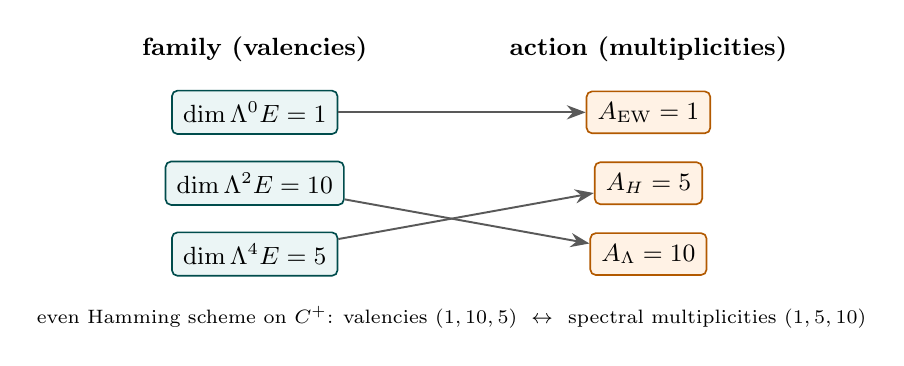
\begin{tikzpicture}[>=Stealth]
  \node[font=\bfseries\small] at (0,1.25) {family (valencies)};
  \node[font=\bfseries\small] at (5.0,1.25) {action (multiplicities)};
  \node[dbox] (v0) at (0,0.45)  {$\dim\Lambda^0E=1$};
  \node[dbox] (v2) at (0,-0.45) {$\dim\Lambda^2E=10$};
  \node[dbox] (v4) at (0,-1.35) {$\dim\Lambda^4E=5$};
  \node[abox] (m0) at (5.0,0.45)  {$A_{\mathrm{EW}}=1$};
  \node[abox] (m1) at (5.0,-0.45) {$A_{H}=5$};
  \node[abox] (m2) at (5.0,-1.35) {$A_{\Lambda}=10$};
  \draw[flow] (v0)--(m0);
  \draw[flow] (v4)--(m1);
  \draw[flow] (v2)--(m2);
  \node[font=\scriptsize] at (2.5,-2.15)
    {even Hamming scheme on $C^+$: valencies $(1,10,5)\ \leftrightarrow\ $ spectral multiplicities $(1,5,10)$};
\end{tikzpicture}
\caption{Exterior--Action duality. The Standard-Model family is the valency side of the even Hamming
scheme on the five-slot code; the cosmological action ladder is its spectral (multiplicity) side. The
$\Lambda$ (pair) sector $\Lambda^2E$ has dimension $\binom52=10$, the origin of the decuple exponent.}
\label{fig:duality}
\end{figure}

\noindent Natural sector assignment:
\[
  \boxed{\ EW\leftrightarrow\Lambda^0E\ (\text{singlet}),\quad
  H\leftrightarrow\Lambda^4E\cong E^\vee\ (\dim5),\quad
  \Lambda\leftrightarrow\Lambda^2E\ (\dim10).\ }
\]
The cosmological constant lives on the \emph{pair} sector $\Lambda^2E$, $\dim=\binom52=10$; this is
why the decuple bridge has exponent $10$ --- $\Lambda$ is a product over all $\binom52$ carrier pairs
($K_5$ edges), not over the full $16$-state family.

\subsection{$\gcar=5$ as the Pascal closure}
A family is exactly the complete Pascal truncation to degree two:
\begin{equation}
  \boxed{\ \dim S^+=2^{\gcar-1}=\binom{\gcar}{0}+\binom{\gcar}{1}+\binom{\gcar}{2}\ \Longleftrightarrow\ \gcar=5\ }
  \qquad(16=1+5+10),\quad\mE,
\end{equation}
the unique positive-integer solution of $f(g):=2^{g-1}-1-\tfrac{g(g+1)}{2}=0$. \emph{Proof of
uniqueness.} Direct evaluation gives $f(1){=}{-1}$, $f(2){=}{-2}$, $f(3){=}{-3}$, $f(4){=}{-3}$,
$f(5){=}0$, $f(6){=}{+10}$; so $g{=}5$ is the only root in $\{1,\dots,6\}$. For $g\ge6$ the forward
difference is $f(g{+}1)-f(g)=2^{g-1}-(g{+}1)\ge 2^{5}-7=25>0$ and increasing, so $f$ is strictly
increasing on $[6,\infty)$ from $f(6){=}10>0$; hence $f(g)>0$ for all $g\ge6$ and there is \emph{no}
further root. Thus $\gcar=5$ is the unique solution (no finite-range caveat). \veri{v2\_carrier\_pascal.py}
This is sharper than $2\gcar=\binom{\gcar}{2}$: the family code (even states, $2^{g-1}$) equals the action
code (sum of the first three Pascal entries) only at $\gcar=5$.

\begin{keybox}[Carrier uniqueness theorem: $\gcar=5$ and the $3{+}2$ split are forced \mE]
The carrier rank and its colour/weak split are not chosen --- they are the unique solutions of two
integer conditions tied to the $E_8$ closure and the SM gauge algebra:
\begin{align}
  &\boxed{\ \gcar=5\ \text{is the unique }g\text{ with } \Nfam=\tfrac{2^{g-1}-1}{g}\in\Z^+\ \text{and}\ \operatorname{rank}E_8=g+\Nfam=8\ }\\[2pt]
  &\boxed{\ (b,s)=(3,2)\ \text{is the unique split of }\ b+s=\gcar=5,\ \ b^2+s^2=13=|R(A_3)|{+}1\ }
\end{align}
The integer-family carriers are $g\in\{3,5,7,\dots\}$ (rank $4,8,16$), so $\operatorname{rank}E_8=8$ picks
$\gcar=5$ uniquely; and $b^2+s^2=13$ with $b{+}s=5$ forces $(3,2)$, reproducing
$\dim\mathfrak g_{\mathrm{SM}}=(b^2{-}1)+(s^2{-}1)+1=12=|R(A_3)|$. The induced hypercharge is anomaly-free
($\operatorname{Tr}Y=\operatorname{Tr}Y^3=0$ over the $16$ states). This hardens P2: the \emph{rank} and
the \emph{split} are forced; only the seam$\to$carrier interface itself remains a declared input.
\veri{v14\_carrier\_uniqueness.py}
\end{keybox}

\par\smallskip\noindent\textbf{The Pascal grammar: one $\Lambda^\bullet$ mechanism in four places (anti-numerology) \mE.}
The recurring small integers are \emph{not} coincidences --- they are the \emph{same} exterior-algebra
(Pascal) mechanism read in four spaces, which is why the binomials of rows $4$ and $5$ keep reappearing:
\[
  \renewcommand{\arraystretch}{1.25}
  \begin{array}{l|l}
  \textbf{space} & \textbf{Pascal reading}\\\hline
  \text{carrier (one generation)} & \dim S^+=\Lambda^{\mathrm{even}}(5)=\tbinom50{+}\tbinom52{+}\tbinom54=1{+}10{+}5=16\\
  \text{scale ladder (cosmology)} & \AEW:\AH:\AL=\tbinom50:\tbinom51:\tbinom52=1:5:10\\
  \text{flavor } u/d\text{ readout} & \|\operatorname{Pl}(K)\|_1=\tbinom40{+}\tbinom41{+}\tbinom42=1{+}4{+}6=11=16{-}\gcar\\
  \text{mass volume} & \det M_{\mathrm{SM}}\sim(\phiz)^{6+9+10}=(\phiz)^{25}=(\phiz)^{\gcar^2}\\
  \end{array}
\]
So the carrier is the even row $5$, the scale ladder is the lower row $5$, the $u/d$ leg is the cumulative
row $4$ up to $\deg u^c=2$, and the mass volume closes on $\gcar^2$. \emph{One} grammar
($\Lambda^k$ of the $5$-slot carrier and the $4=|\mu_4|$ family fundamental), not four lucky hits.
\veri{v44\_carrier\_exterior.py}\,\allowbreak\veri{v45\_family\_exterior.py}\,\allowbreak\veri{v46\_grand\_mass\_volume.py}
\par\smallskip

\subsection{One master moment generates $40$, $41$, $240$, $\dtwo$}
With $X=6Y$, the quadratic hypercharge trace on one family is $\operatorname{Tr}_{S^+}X^2=120=5!$,
and it generates the whole integer chain:
\begin{equation}
\begin{gathered}
  \sum_{f,j}L_{f,j}=\frac{\operatorname{Tr}_{S^+}X^2}{3}=40,\qquad
  10b_1=\frac{\operatorname{Tr}_{S^+}X^2}{3}+1=41,\\[2pt]
  |R(E_8)|=2\operatorname{Tr}_{S^+}X^2=240,\qquad
  \dtwo=4!\,\operatorname{Tr}_{S^+}X^2\,\cthree^8 .
\end{gathered}
\end{equation}
The flavor budget, the $U(1)$ budget, the $E_8$ count and the second seam defect all hang on the
second hypercharge moment $5!$. \mE\ \emph{Round-22 sharpening:} the moment itself is one symbolic
identity, $\operatorname{Tr}_{S^+}X^2=4|X|^2=4h(E_8)=120$ --- the Coxeter number carries the whole
chain (\veri{v810\_cutcode\_moment.py}) \mE.

\subsection{Compact $E_8$ compression and the role of $\nu^c$}
\begin{equation}
  \boxed{\ \begin{aligned}
    |R(E_8)|&=\dim S^+\cdot\gcar\cdot\Nfam=16\cdot5\cdot3=240,\\
    \dim E_8&=\dim S^+(\AH+\AL)+(\gcar+\Nfam)=240+8=248
  \end{aligned}\ }
\end{equation}
with $\Nfam=(2^{\gcar-1}-1)/\gcar=15/5=3$ and $\operatorname{rank}E_8=\gcar+\Nfam=8$. \mE. The
right-handed neutrino $\nu^c$ is the Pascal singleton $\Lambda^0E=(1,1)_0$ that closes $16=1+5+10$;
removing it breaks the truncation and shifts $\alpha^{-1}$ by $2.16\times10^{-3}$.

% =====================================================================
\section{The $D_5\times A_3$ compiler: $E_8$ as a closure, not an input}
\label{sec:d5a3}
% =====================================================================
This section upgrades the $E_8$ atlas (Section~\ref{sec:e8}) from a counting coincidence to an explicit
lattice construction. The whole content is consolidated and verified in the standalone companion note
\emph{``The Even Carrier Code and the $\mathbb Z_{30}$ Coxeter Compiler.''} The thesis: the carrier
code is the $D_5$ half-spinor, the family geometry is an $A_3$, and $E_8$ is the standard unimodular
glue closure of $D_5\oplus A_3$ --- with the four punctures $\mu_4$ as the glue code.

\TFPTeightglue

\par\smallskip\noindent\textbf{The compiler in one line:}
\begin{keyeq}
$\displaystyle \text{five carrier slots}\Rightarrow D_5,\quad
  \text{four family corners }\mu_4\Rightarrow A_3,\quad
  (D_5\oplus A_3)+\mu_4\text{-glue}\Rightarrow E_8.$
\end{keyeq}

\begin{figure}[ht]
\centering
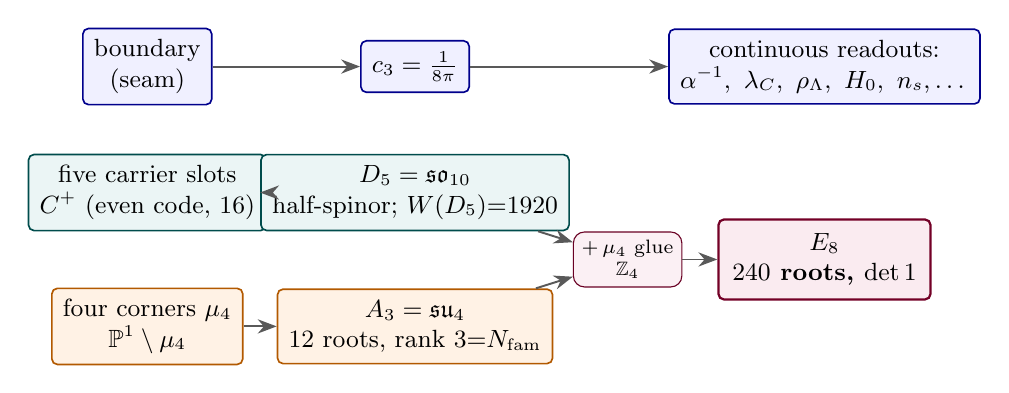
\begin{tikzpicture}[>=Stealth]
  \node[cbox] (seam) at (0,2)    {boundary\\(seam)};
  \node[cbox] (c3)   at (3.4,2)  {$c_3=\tfrac1{8\pi}$};
  \node[cbox] (cont) at (8.6,2)  {continuous readouts:\\$\alpha^{-1},\ \lambda_C,\ \rho_\Lambda,\ H_0,\ n_s,\dots$};
  \node[dbox] (slots) at (0,0.4)  {five carrier slots\\$C^+$ (even code, $16$)};
  \node[dbox] (d5)    at (3.4,0.4){$D_5=\mathfrak{so}_{10}$\\half-spinor; $W(D_5){=}1920$};
  \node[abox] (corn)  at (0,-1.3) {four corners $\mu_4$\\$\mathbb P^1\setminus\mu_4$};
  \node[abox] (a3)    at (3.4,-1.3){$A_3=\mathfrak{su}_4$\\$12$ roots, rank $3{=}N_{\mathrm{fam}}$};
  \node[draw=purple!55!black, fill=purple!6, rounded corners, align=center,
        font=\scriptsize, inner sep=3pt] (glue) at (6.1,-0.45) {$+\,\mu_4$ glue\\$\mathbb Z_4$};
  \node[ebox] (e8) at (8.6,-0.45) {$E_8$\\$240$ roots, $\det 1$};
  \draw[flow] (seam)--(c3);   \draw[flow] (c3)--(cont);
  \draw[flow] (slots)--(d5);  \draw[flow] (corn)--(a3);
  \draw[flow] (d5)--(glue);   \draw[flow] (a3)--(glue);  \draw[flow] (glue)--(e8);
\end{tikzpicture}
\caption{The explanation hierarchy. The boundary fixes the seam seed $c_3$; the five-slot even
carrier code is the $D_5$ half-spinor; the four punctures $\mu_4$ give $A_3$; their common
$\mathbb Z_4$ discriminant ($\mu_4$) glues $D_5\oplus A_3$ into the unimodular $E_8$. $E_8$ is the
\emph{closure}, not the input; $c_3$ dresses the continuous observables.}
\label{fig:pipeline}
\end{figure}

\par\smallskip\noindent\textbf{The glue is \emph{one} operation in two categories.} The same
order-$|\mu_4|{=}4$ discriminant glue closes $D_5\oplus A_3$ into $E_8$ \emph{twice over}: once on
\emph{root lattices} (the unimodular pushout $D_5\oplus A_3+\mu_4\Rightarrow E_8$, \vref{v1}) and once on
\emph{chiral conformal nets} (the simple-current / anyon-condensation extension
$(D_5)_1\otimes(A_3)_1\rtimes\mu_4\cong(E_8)_1$, \vref{v92}/\vref{v281}). These are not two coincidences but
the two functorial faces of a single commuting square (\vref{v234}/\vref{v277}/\vref{v260}); the boundary
realisation on which the strict-TOE residual turns (\texttt{SEAM.EQUIV.01}) is exactly the statement that the
raw seam realises this square --- now \emph{closed modulo cited theorems on its MMST route}
\texttt{SEAM.EQUIV.MMST.01} (the lattice/$S_3$ stack pins it at
every computable level, Lean \texttt{FORM.SEAM.MMST.01}; only the cited MMST/OS continuum-existence theorems stay
\mO, \vref{v367}/\vref{v368}/\vref{v376}--\vref{v379}/\vref{v336}; the twistor route
\texttt{SEAM.EQUIV.TWISTOR.01} and the unconditional parent stay \mO). The extension leg of that citation package is
itself re-founded at net level (\veri{v469\_seam\_crossedproduct\_route.py}): the $128$-spinor step is the
\emph{local} $\Z_2$ simple-current crossed product ($h_s(SO(16)_1)=16/16=1\in\Z$, the Longo--Rehren locality
criterion; KLM $\mu=4/2^2=1$), on 1995--2001 peer-reviewed subfactor theory, with the lattice-VOA preprint route
demoted to an independent second witness, and the realisation input reduced to invariant level (R1$'$).
Premise (i) of that package ($c_-{=}8$) now also carries a \emph{ground-state} witness
(\veri{v489\_seam\_modular\_commutator.py}): the Kim--Shehab--Kim modular commutator
$J(A,B,C)=(\pi/3)c_-$, evaluated on the exact BdG ground state of the collar model, gives $c_-=8=\gcar+\Nfam$
for the $16$-layer carrier (per layer $0.500000$ at $L{=}48$; trivial and orientation-flip controls pass) ---
independent of both the Chern route (\vref{v367}) and the KLM count (\vref{v378}).
\texttt{SEAM.EQUIV.01} stays \mO.
\emph{Follow-up (2026-08-03, the $G_{\mathrm{net}}$ witnesses):} the
index-$4$ statement now carries two \emph{exact} arithmetic/index
witnesses.  The NS/R grading \emph{is} the parity character of
$E_8(\Z[i])/(1{+}i)=\mathbb F_2^4$ --- $(1{+}i)L$ lies in the even
sublattice (proved on a $\Z$-basis), all $15\times16$ root classes
are parity-pure ($7$ NS $+$ $8$ R), so the Ramond projection is
$(1{+}i)$-\emph{adic} at the one ramified edge of the
$\Z[i]$-E8 Hecke tower (\veri{v722\_phys\_ramified\_ns\_r.py},
$9/9$, \textsc{ramified-sees-nsr}); and on the CAR ladder the
$\mu_4$-average expectation has optimal Pimsner--Popa constant
exactly $1/4$ and Watatani index exactly $4$ via an explicit
quasi-basis with \emph{forced} weights, with $\mu_4$ \emph{derived}
from the clock and the Ramond sector healed state-preservingly by
the Klein zero-mode dressing (\veri{v726\_phys\_car\_pp\_index.py},
$57/57$, \textsc{t2-slice-go}).  The remaining half is the
\emph{identification} of the ladder Q-system with the constructed
$\mathbb C[\Z_4]$ object (\texttt{GNET.RAMIFIED.01}, kills
registered); \texttt{GATE.METRIC.08}/\texttt{.10} typing unchanged.
\emph{Follow-up (2026-08-05, the continuum strand):} the
finite-level precursors of the GNS limit are measured
\emph{coherent} (\veri{v779\_gnet\_gns\_arf.py}, $27/27+27/27$):
the Haar scaling tower intertwines exactly, the index-4
expectation squares commute exactly (the finite half of the
Q-system identification), the state converges geometrically, and
the exact dim law $d_c(\ell)=4^{\ell-1}+2^{\ell-1}\cos(\pi c/2)$
types the $\mathbb C[\Z_4]$ obstruction at exactly $2^{-\ell}$
(explaining the $\ell=1$ three-sector anomaly); the honest
negative: the $16=1{+}5{+}10$ counting echo with the Arf geometry
is exact but \emph{non-geometric}, and the two fours (index $4$
vs channel $4/49$) stay in their registers.  The round-21
martingale probe measures the limit-existence hypotheses of the
continuum strand as met
(\veri{v802\_gnet\_martingale.py}, $15/15$,
\textsc{martingale-hypotheses-met}; the analytic remainder stays
typed).  Typing unchanged.

\TFPTdoublepushout

\subsection{Carrier $=D_5=\mathfrak{so}_{10}$ (proved)}
The $16$ even-occupation states $C^+=\{x\in\mathbb F_2^{\gcar}:|x|\ \text{even}\}$ are exactly the
weights of the $D_5$ half-spinor $\tfrac12(\pm1,\dots,\pm1)$ (even number of minus signs). The
flip-weight-$4$ relation is the \textbf{Clebsch graph} $\mathrm{SRG}(16,5,0,2)$ and the flip-weight-$2$
relation is its complement $\mathrm{SRG}(16,10,6,6)$; the \emph{affine} automorphism group of the scheme
(translations $\rtimes$ coordinate permutations) is the $D_5$ Weyl group,
\begin{equation}
  \boxed{\ \operatorname{Aut}_{\mathrm{aff}}(C^+)=C^+\rtimes S_5,\quad |\operatorname{Aut}_{\mathrm{aff}}(C^+)|=2^{\gcar-1}\gcar!=1920=|W(D_5)|=r\,|R(E_8)|\ }\qquad\mE ,
\end{equation}
(the linear code automorphism group alone is only $S_5$; the order-$1920$ group is the affine/scheme one)
and the Clebsch edge count is the flavor budget $|E(R_4)|=\tfrac{16\cdot5}{2}=40=|R(D_5)|=\sum_{f,j}L_{f,j}$.
\emph{Round-22 grading (2026-08-06):} the Arf split $16=1+\bar5+10$ \emph{is} the cut
classification $(0|5)+(1|4)+(2|3)$ of $K_5$ (the cut map injective-isometric on all $256$ cells),
and the Clebsch edges grade as $40=5+20+15$ over the Arf shells with the within-$10$ block equal to
the Petersen graph --- an Arf/cut geometry, exact but carrying no matter semantics
(\veri{v810\_cutcode\_moment.py}) \mE.

\subsection{Family $=A_3=\mathfrak{su}_4$ from $\mathbb P^1\setminus\mu_4$ (proved, with the metric settled)}
The carrier geometry fixes $X_f^\circ\cong\mathbb P^1\setminus\mu_4$, $H_1=\mathbb Z^3$, rigid $D_4$ generated by
$z\mapsto iz,\ z\mapsto1/z$. The twelve puncture-difference cycles $\gamma_i-\gamma_j$ carry the
residue pairing $\operatorname{Res}(\omega_i,\gamma_j)=\delta_{ij}$ and form the $A_3$ root system:
\begin{equation}
  \boxed{\ \#\{\gamma_i-\gamma_j\}=12=|R(A_3)|=\dimg,\quad \operatorname{rank}=3=\Nfam,\quad
  \mathrm{Gram}=\mathrm{Cartan}(A_3),\ \det=4\ }\qquad\mE .
\end{equation}
The corner rotation $z\mapsto iz$ acts on $H^1=\mathbb C^3$ as the $A_3$ Coxeter element (order
$4=h(A_3)=|\mu_4|$, spectrum $\{i,-1,-i\}$, $\chi=\Phi_4\Phi_2$), an isometry of the Cartan form ---
the exact analogue of the $E_8$ Coxeter element reading $\Phi_{30}$.
\par\smallskip\noindent\textbf{The $\mu_4$ clock is the order-$4$ character of the $E_8$ cycle, and $(2,3,5)$
is the icosahedron (\veri{v223\_coxeter\_totative\_clock.py}, \veri{v219\_icosahedral\_mckay.py}).} The two
``Coxeter'' clocks are one object read at two scales. The $E_8$ exponents are the totatives
$(\Z/30)^\times=\{1,7,11,13,17,19,23,29\}$, and the multiplicative order-$4$ element $7$ ($7^2{=}19$,
$7^4{=}1\bmod30$) generates a literal $\mu_4$ clock $\langle7\rangle=\{1,7,13,19\}$ that permutes the four
conjugate Coxeter $2$-planes --- the same $\mu_4$ as the seam corner rotation. And the period
$30=2{\cdot}3{\cdot}5$ itself is not a free factorisation: by the McKay correspondence $E_8$ is the
exceptional \emph{top} of the tower of finite $SU(2)$ subgroups ($2T{\to}\hat E_6$, $2O{\to}\hat E_7$,
$2I{\to}\hat E_8$), so its branch data is the \emph{icosahedron} and the three atoms $(|\Z_2|,\Nfam,\gcar)
=(2,3,5)$ are its rotation-axis orders. The binary icosahedral group $2I$ (order $120=|R^+(E_8)|$) has nine
irreducible-representation degrees $\{1,2,2,3,3,4,4,5,6\}$ equal to the affine-$E_8$ Kac marks, with
$\sum d_i=30=h(E_8)$ and $\sum d_i^2=120$. This is a \emph{backward certificate} of the closed $E_8$ \mE\
(it explains the $(2,3,5)$ choice \mC; it does \emph{not} replace the P2 input).
\par\smallskip\noindent\textbf{The metric, settled (former \mC).}
The transcendental geometric (Green) metric $G_{ij}=-\log|p_i-p_j|$ on $\mu_4$ is only
$D_4$-symmetric, with a regularisation-independent anisotropy $-\log2$ on the root space, so it is
\emph{not} proportional to the $A_3$ Cartan form. But it does not need to be: the $E_8$-relevant $A_3$
is the canonical \emph{residue} pairing (integral, $S_4$-symmetric, $=\mathrm{Cartan}(A_3)$), and the
geometric metric is a $D_4$-equivariant deformation preserving the root system, Weyl group and Coxeter
element. So the lattice structure is exact \mE; the analytic metric is a characterised deformation,
not an open gap.
\par\smallskip

\subsection{The $\mu_4$ glue and the $5/4+3/4=2$ discriminant theorem (proved)}
The two factors have equal discriminant groups and $E_8$ is unimodular, so the glue index is exactly
$|\mu_4|$:
\begin{equation}
  \operatorname{disc}(D_5)=\operatorname{disc}(A_3)=\mathbb Z_4,\qquad
  [E_8:D_5\oplus A_3]=\sqrt{\tfrac{\det D_5\det A_3}{\det E_8}}=\sqrt{\tfrac{4\cdot4}{1}}=4=|\mu_4| .
\end{equation}
The discriminant-form norms sum to the $E_8$ root norm, and --- strikingly --- they are pre-existing
TFPT constants:
\begin{equation}
  \boxed{\ \begin{aligned}
    &q(D_5)=\tfrac54=\frac{\dtwo}{\dtop^2},\qquad q(A_3)=\tfrac34=\xi_{\mathrm{tree}},\\
    &q(D_5)+q(A_3)=2=|\text{$E_8$ root}|^2
  \end{aligned}\ }\qquad\mE\ \veri{v1\_e8\_glue.py}
\end{equation}
This is literally the $E_8$ spinor-root split $\tfrac12(\pm)^8=\tfrac12(\pm)^5\oplus\tfrac12(\pm)^3$,
$5\cdot\tfrac14+3\cdot\tfrac14=2$.

\begin{figure}[ht]
\centering
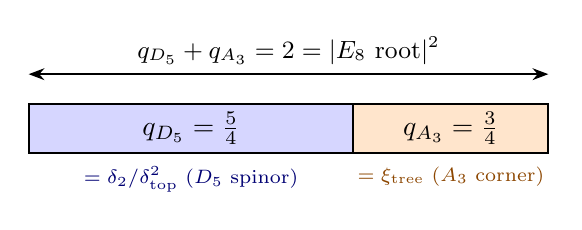
\begin{tikzpicture}[>=Stealth]
  \def\sc{3.3}
  \fill[blue!16]   (0,0) rectangle ({1.25*\sc},0.62);
  \fill[orange!20] ({1.25*\sc},0) rectangle ({2*\sc},0.62);
  \draw[line width=0.7pt] (0,0) rectangle ({2*\sc},0.62);
  \draw[line width=0.7pt] ({1.25*\sc},0)--({1.25*\sc},0.62);
  \node at ({0.625*\sc},0.31) {$q_{D_5}=\tfrac54$};
  \node at ({1.625*\sc},0.31) {$q_{A_3}=\tfrac34$};
  \node[below, font=\scriptsize, text=blue!45!black]   at ({0.625*\sc},-0.05) {$=\delta_2/\delta_{\mathrm{top}}^2$ ($D_5$ spinor)};
  \node[below, font=\scriptsize, text=orange!55!black] at ({1.625*\sc},-0.05) {$=\xi_{\mathrm{tree}}$ ($A_3$ corner)};
  \draw[{Stealth}-{Stealth}, line width=0.6pt] (0,1.0)--({2*\sc},1.0);
  \node[above, font=\small] at ({\sc},1.0) {$q_{D_5}+q_{A_3}=2=|E_8\ \text{root}|^2$};
\end{tikzpicture}
\caption{The discriminant-norm glue. The $E_8$ spinor root $\tfrac12(\pm)^8$ (norm $2$) splits across
$D_5\times A_3$ as $5\cdot\tfrac14+3\cdot\tfrac14$; the two halves are the pre-existing TFPT constants
$\delta_2/\delta_{\mathrm{top}}^2=\tfrac54$ and $\xi_{\mathrm{tree}}=\tfrac34$.}
\label{fig:gluenorm}
\end{figure}

\noindent The standard branching is realised explicitly:
\begin{equation}
  \mathfrak e_8=(45,1)\oplus(1,15)\oplus(10,6)\oplus(16,4)\oplus(\overline{16},\overline4),\qquad
  248=45{+}15{+}60{+}64{+}64,\quad 240=40{+}12{+}60{+}64{+}64 ,
\end{equation}

\begin{figure}[ht]
\centering
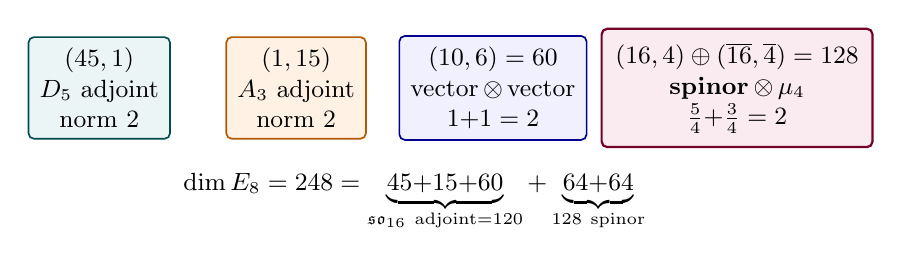
\begin{tikzpicture}[>=Stealth]
  \node[dbox] (b1) at (0,0)    {$(45,1)$\\$D_5$ adjoint\\norm $2$};
  \node[abox] (b2) at (2.5,0)  {$(1,15)$\\$A_3$ adjoint\\norm $2$};
  \node[cbox] (b3) at (5.0,0)  {$(10,6)=60$\\vector\,$\otimes$\,vector\\$1{+}1=2$};
  \node[ebox] (b4) at (8.1,0)  {$(16,4)\oplus(\overline{16},\overline4)=128$\\spinor\,$\otimes\,\mu_4$\\$\tfrac54{+}\tfrac34=2$};
  \node[font=\small] at (4.0,-1.45)
    {$\dim E_8=248=\underbrace{45{+}15{+}60}_{\mathfrak{so}_{16}\ \mathrm{adjoint}=120}+\underbrace{64{+}64}_{128\ \mathrm{spinor}}$};
\end{tikzpicture}
\caption{The $E_8\supset D_5\times A_3$ branching as norm-$2$ blocks. The adjoint half is the
hypercharge moment $\operatorname{Tr}_{S^+}X^2=120=\dim\mathfrak{so}_{16}$; the spinor half is two
sheets over the four corners $\mu_4$.}
\label{fig:e8blocks}
\end{figure}
and assembling $D_5\oplus D_3\subset D_8$ with the even spinor coset produces all $240$ roots
(norm $2$, Cartan $\det=1$, every root an integer combination of one simple-root basis): \emph{the
$240$-metrisation is no longer blind --- $E_8$ is built}. \mE

\par\smallskip\noindent\textbf{Hecke structure of the glue census is lattice-native
(\texttt{HECKE.GEOM.01}).}
The $\mu_4$-glue class thetas that refine the $240$-root branching ($240=52{+}64{+}60{+}64$ over
$\Z/4$) now carry a machine-checked Hecke package
(\veri{v535\_hecke\_from\_geometry.py}): Kneser $p$-neighbours realise
$\#\mathrm{iso\_lines}=\sigma_3(p)\,\#\mathbb P^3(\mathbb F_p)$ at $p=2,3,5,7$; the marked
neighbour-sum is the affine element $\nu_p=a\,\mathrm{Id}+b\,T_p$ with cusp output
$a_3=-4$, $a_5=-2$; and the seven census $q$-series span exactly the $2$-adic oldform hull of
$E_4$ and $f_8$ (levels $\{1,2,4,8,16\}$ and $\{8,16\}$). Classical scaffolding named classical;
weight-$4\to$GL$(1)$ stays \mO; no RH claim. \mE\ (in-suite mechanics)

\par\smallskip\noindent\textbf{Eichler trace layer at the $E_8$ lattice
(\texttt{HECKE.GEOM.EICHLER.01}).}
The same census channels now carry a machine-checked Eichler/Witt package
(\veri{v536\_eichler\_trace\_layer.py}; $23$ checks, $\sim30$\,s; builds on
\texttt{HECKE.GEOM.01} without duplicating Kneser/$\nu_p$/oldform checks).
\emph{(A)} The elementary Witt shadow
$\lambda_{\mathrm{Eis}}=\sigma_3(\#\mathbb P^3-\sigma_3)=L-\sigma_3^2$ is closed in $p$
(identically and for all odd $p\le100$).
\emph{(B)} The Eichler identity $\lambda_{\mathrm{geom}}=\lambda_{\mathrm{Eis}}+a_p^2$ is
two-sided at $p=3$ (live type-(i)/(ii) split: $352=364-12$) and at $p=5$ via a T36-validated
freeze ($3784=3906-122$); the assembler $R(p)=\sigma_3-1-c(p^2)/8$ equals $a_p^2$ with
Kneser filter $=$ identity.
\emph{(C)} Closed Type-A/B local densities
$N_A=\min\bigl(240(1+p^3),\,p^7+p^4-p^3-1\bigr)$ (B empty iff $p^4<241$; $p=7$ live
$82560/743040$; injectivity at $p=11,13$).
\emph{(D)} Signed extraction $a_p=-c(p)/8$ from geometric $\mathrm{Shell}(p)$ recovers
$(-4,-2,+24)$ and $b\in\{24,124,368\}$.
\emph{(E)} $O(1)$ assembler for all odd $p\le31$ against the eta product $f_8$.
Classical Eichler/Siegel/Witt named classical; the claim is in-suite two-sidedness and the
closed compiler densities. Honest fences: $\mathrm{Shell}(p^2)$ for $p\ge7$ out of scope;
fibre refinement scoped to $\{5,7,11\}$; weight-$4\to$GL$(1)$ stays \mO; no RH claim; no
marker moves. \mE\ (mechanics) / \mO\ (weight drop)

\par\smallskip\noindent\textbf{Half-integral bridge
(\texttt{HECKE.GEOM.HALFINT.01}).}
The weight-$4$ cusp $f_8$ now has a machine-checked half-integral companion in the compiler
theta-monoid (\veri{v537\_halfintegral\_bridge.py}; $20$ checks, $\sim90$\,s; companion to
\texttt{HECKE.GEOM.01}/\texttt{HECKE.GEOM.EICHLER.01}).
\emph{(A)} In the $70$-element weight-$5/2$ theta-monoid (plain and $q^2$-scaled
$\vartheta_2,\vartheta_3,\vartheta_4$) there is exactly one object with the signed Shimura
identity $\mathrm{Sh}_{t=2,\psi=1}(g)=-8\,f_8$ (witness
$g=\vartheta_2(q^2)^2\,\vartheta_3(q^2)\,\vartheta_4\,\vartheta_4(q^2)$, verified
coefficientwise through $n\le120$; three further monoid elements lift to scales
$+8,-16,+16$).
\emph{(B)} $g$ is an exact $T(p^2)$-eigenform of weight $5/2$, trivial nebentypus, with
eigenvalues $a_p(f_8)$ for $p=3,5,7,11,13$ ($-4,-2,24,-44,22$); trial FE of the
$5/2$-side around centre $5/4$ with $N=512$, $\varepsilon=+1$.
\emph{(C)} $U_4(g)=0$ exactly (mass mod~$4$ supported on $\{1,2\}$); level $32=4\cdot8$
with $M=8$ even lies outside Kohnen~$1982$ --- the plus-route is structurally closed
(negative result part of the claim).
\emph{(D)} With AFE-based twist $L$-values
($\varepsilon_d=\chi_d(8)$; $\varepsilon=-1\Rightarrow L(2)=0$), the Waldspurger quotient
$R(d)=b(|d|)^2\big/\bigl(|d|^{3/2}L(f_8\times\chi_d,2)\bigr)$ is constant on ten
fundamental discriminants $d\equiv1\pmod8$ ($R=23.1873585645\ldots$, relative spread
$\le10^{-12}$, including $d=89$); the class $d\equiv5\pmod8$ vanishes structurally.
Classical Shimura/Kohnen/Waldspurger/Baruch--Mao named classical; the claim is the unique
signed-scale monoid preimage, the in-suite chain, and the \emph{measured} constant $R$.
Honest fences: GL$(2)$ centre $s=2$, not the $\xi$-line; no RH claim;
\texttt{ZETA.HP.CARRIER} untouched; no marker moves.
\mE\ (Shimura/Hecke/Kohnen fence) / \mC\ (measured $R$)

\par\smallskip\noindent\textbf{Compiler relative-trace identity
(\texttt{HECKE.GEOM.RTF.01}).}
The three preceding packages are machine-checked as three \emph{projections} of one finite
relative-trace identity
$[\text{$E_8$/glue orbital counting}]=[\text{Newform/Waldspurger spectral sum}]$
(\veri{v538\_relative\_trace\_identity.py}; $18$ checks, $\sim14$\,s; promotion of discovery
T53; companion to \texttt{HECKE.GEOM.01}/\allowbreak\texttt{HECKE.GEOM.EICHLER.01}/\allowbreak\texttt{HECKE.GEOM.HALFINT.01}).
\emph{(R1)} $\operatorname{Tr}_V(\nu_p\circ\pi)$ is computed \emph{both sides independently}:
geometric $a_p=-c(p)/8$ from the glue census (no modular input) equals spectral $a_p$ from
$\eta(2\tau)^4\eta(4\tau)^4$ (no geometry) for all
$(p,\pi)\in\{3,5,7\}\times\{\mathrm{Id},\pi_{\mathrm{Eis}},\pi_{\mathrm{cusp}},\pi_{E_4},\pi_{f_8}\}$
(anchors e.g.\ $p{=}7$: full trace $727680$, $f_8$-channel $19840$).
\emph{(R2)} The Eichler split $\lambda_{\mathrm{geom}}=\lambda_{\mathrm{Eis}}+a_p^2$
\emph{is} the RTF orbit decomposition (principal orbit $\to\lambda_{\mathrm{Eis}}=L-\sigma_3^2$;
elliptic $\to a_p^2$; cross terms cancel; anchors
$\lambda_{\mathrm{Eis}}=336/3780/19264$, $a_p^2=16/4/576$).
\emph{(R3)} The period side is lattice counting: $g$ is the quaternary form
$n=(x^2+y^2)/2+2z^2+u^2+2w^2$ ($x,y$ odd; sign $(-1)^{|u|+|w|}$), with
$b_{\mathrm{rep}}=b$ through $n\le200$, and
$[\text{signed lattice count}]^2=R\cdot|d|^{3/2}\cdot L(f_8\times\chi_d,2)$ at
$R=23.1873585645$ (rel~$\sim10^{-12}$). Verdict \texttt{ONE-FORMULA}.
Classical Jacquet-type RTF / Eichler / Witt / Waldspurger / theta correspondence named
classical; NEW is the compiler-native realisation and bilateral independence.
Honest fences: the identity is \emph{finite} ($p\in\{3,5,7\}$, finite $d$-windows); the
\emph{infinite} RTF (sum over all $p$ and $d$ $+$ archimedean term) remains the named open
step; no RH claim; not \texttt{ZETA.HP.CARRIER}-relevant; no marker moves.
\mE\ (R1/R2 exact) / \mC\ (R3 measured $R$)

\par\smallskip\noindent\textbf{Weil structure of the compiler family
(\texttt{RTF.GNS.WEIL.01}).}
The compiler family carries a fully identified Weil structure up to
\emph{two explicitly isolated obstructions}
(\veri{v539\_weil\_structure\_family.py}; $25$ checks, $\sim6$\,s; promotion of discovery
T55/T61/T62/T63; companion to \texttt{HECKE.GEOM.RTF.01}).
\emph{(A)} The canonical GNS pairing is the direct integral over the Gelfand spectrum of
the character subalgebra: metric $\ell^2(d,b^2/|d|)$ diagonal; fibres
$\sigma(d)=(\chi_d(3),\ldots,\chi_d(13))$ partition the live family; $\Lambda_{\mathrm{fam}}$
constant on each fibre; twist-mixing certificate per fibre
$\le5.037\times10^{-16}<10^{-12}$.
\emph{(B)} The trivial Sato--Tate isotype is algebraically the GL$(1)$ core
$G_0=(1+Y)/(1-Y)=\zeta_p(w-3)^2/\zeta_p(2w-6)$, globally
$\zeta(u)^2/\zeta(2u)=\sum 2^{\omega(n)}n^{-u}$ (Dirichlet coefficients exact through
$n\le2000$; character expansions
$\Phi_1=\chi_0+\chi_2$, $\Phi_2=\chi_4-\chi_2$, $\Phi_3=2\chi_0-\chi_4+\chi_6$,
$\Phi_4=\chi_8-\chi_6$; core series $c_{k,0}=[1,0,2,0,2,0]$).
\emph{(C)} The family form satisfies the exact linear relation
$Q_{\mathrm{fam}}=2Q_\zeta(g)-2Q_\zeta(g_\flat)+\mathrm{Arch}+\mathrm{Corr}$
($\mathrm{Prime}_F=2P_\zeta(g)-2P_\zeta(g_\flat)$ with max rel~$9\times10^{-16}$;
$Q_{\mathrm{fam}}=Q_F+\mathrm{Corr}$ with rel~$2\times10^{-16}$).
\textbf{Obstruction 1:} the doubling term enters with a \emph{minus}
(family positivity does \emph{not} imply $Q_\zeta\ge0$).
\textbf{Obstruction 2:} the Plancherel correction is demonstrably non-automorphic
(no polar/arch absorption; no finite Euler factor; identified as
$e^{-\sum p^{-u}}$-type).
Finite-class positivity $Q_{\mathrm{fam}}\in[4.369,11.486]$ is measured \mC;
dense-class positivity stays open / RH-adjacent and is \emph{not} claimed.
Classical Weil 1952 / Gelfand / SU$(2)$--Chebyshev / Sato--Tate / $2^\omega$-series / GNS
named classical; NEW is the compiler-native identification and the machine-checked
isolation of the two obstructions.
Honest fences: \emph{not} ``almost RH'' --- the claim structurally shows why family
positivity does not imply RH; \texttt{ZETA.HP.CARRIER} untouched; no marker moves.
\mE\ (A/B/C/obstructions exact) / \mC\ (finite-class $Q_{\mathrm{fam}}$)

\par\smallskip\noindent\textbf{Amplitude route and positive linear carrier
(\texttt{RTF.GNS.AMP.01}).}
The route out of the square plane behind the two \texttt{RTF.GNS.WEIL.01}
obstructions is now machine-checked
(\veri{v540\_amplitude\_linear\_carrier.py}; $34$ checks, $\sim3$\,s; promotion of
discovery T67--T72; companion to
\texttt{HECKE.GEOM.RTF.01}/\texttt{RTF.GNS.WEIL.01}).
\emph{(A)} The amplitude Dirac
$D=\bigl(\begin{smallmatrix}0&V\\V^{\mathsf T}&0\end{smallmatrix}\bigr)$ with
$V[d,m]=\sqrt{w_d}\,b(d)\,\chi_d(m)$, $w_d=|d|^{-1}$, exists exactly and is
Hecke-equivariant: $D=D^{\mathsf T}$,
$D^2=\operatorname{diag}(VV^{\mathsf T},K)$ with $V^{\mathsf T}V=K$
(rel $2.7\times10^{-16}$), spectral $\pm$-symmetry; $m$-side intertwining
$VA_p^{\mathsf T}=\hat A_pV$ exact on the $p$-free locus ($p=3,5,7$) and $d$-side
Shimura $b(dp^2)=b(d)\,(a_p-\chi_d(p)p)$ integer-exact on $644$ pairs.
\emph{(B)} The geometric polarisation $b=N_+-N_-$ is exact (parity-split lattice
count of the quinary form, plus the $\Theta$-monomial identity coefficientwise);
$\Theta=N_++N_-$ is a \emph{pure} Siegel--Weil Eisenstein $T(p^2)$-eigenform with
eigenvalues $\sigma_3(p)=1+p^3$ ($p\le13$ exact; cusp component zero), carrying the
Cohen seed identity $\Theta(d)=-48\,L(-1,\chi_d)$ exact-rational on $159$ live $d$
(Cohen 1975: $H(2,d)=L(-1,\chi_d)$; generalised Bernoulli $B_{2,\chi}$).
\emph{(C)} Every coefficient bilinear form inherits the even-$k$ deletion: the
Cauchy--Littlewood window lemma with \emph{free} Satake symbols has numerator
$1-stuv\,X^2$, hence $1-p^6X^2$ pair-independently at $st=uv=p^3$ (five channels
checked); simultaneously the deletion \emph{is} the square-class double counting of
the towers, $\mathrm{fam}\,[1,0,2,0]+2\flat\,[0,2,0,2]+\delta_{k1}=[2,2,2,2]$
(generating-function exact; M\"obius square sieve).
\emph{(D)} The positive linear carrier $\ell^2(d,\mu)$ with
$\mu=48\,|L(-1,\chi_d)|\,|d|^{-a}$ carries \emph{full} weights
$\lambda_k=1+p^{3k}-(\chi p)^k$ (layer $[1,1,1,1]$; no even-$k$ kill) and the plus
balance $Q=Q_\zeta(g_-)+Q_\zeta(g_+)$, $g_\pm=e^{\pm3u/2}g$
(rel $2\times10^{-15}$); the $\flat$/doubling kernel enters \emph{with plus} ---
the sign of the v539 minus inverted.
\emph{(E)} The completed functional equation
$\Lambda_\Theta(s)=8^{1-s}\,\Lambda_{\Theta^\dagger}(5/2-s)$ holds exactly
(Fricke closed via the Jacobi inversions; rel $\sim10^{-40}$ modular and in the
strip; poles $5/2$ and $0$ swapped; centre $5/4$, plus-balance locus off-centre by
exactly $1/4$); the guaranteed cone and the gap functional are
FE-self-dual/-covariant.
\textbf{Open boundary as content:} the positivity is \emph{Euler-region} positivity
(edge $L$-values, not the central line); the residual distance to the Weil cone is
the FE-covariant gap functional $\lambda^*$ on $n\equiv6\pmod 8$ --- named,
measured, Farkas-certified, and not removable by any finite signed theta library.
Classical Cohen 1975 / Siegel--Weil / Jacobi--Fricke / Landen / Hecke split-Mellin /
Cauchy--Littlewood / Shintani / Weil 1952 / Farkas named classical; NEW is the
compiler-native consolidation.
Honest fences: \emph{not} ``almost RH''; \texttt{ZETA.HP.CARRIER} untouched;
no marker moves.
\mE\ (A--E exact) / \mC\ (sampled cone facts; $\lambda^*$ named open)

\par\smallskip\noindent\textbf{Matching lemma and transport ledger package
(\texttt{RTF.GNS.LEDGER.01}).}
The discovery proof package T78--T85 is now load-bearing as one module in which
every core check is \emph{recomputed}, not cited
(\veri{v541\_matching\_lemma\_ledger.py}; $33$ checks, $\sim10$\,s; companion to
\texttt{HECKE.GEOM.RTF.01}/\texttt{RTF.GNS.WEIL.01}/\texttt{RTF.GNS.AMP.01}).
\emph{(A) Window proof.} The matching lemma of the hybrid certificate recipe is
\emph{proved exact-integer on $[4,10^6]$}: the certificate $7S(j)<40A(j)$
(i.e.\ $\rho_{\mathrm{design}}F(j)<1$ with $\rho=21/20$) holds at \emph{every}
atom $j\le10^6$ ($0$ violations over $939\,870$ clash atoms; full enumeration,
proven no-overflow, big-integer rechecks), with the exact Fraction margin
$X=22242575693/270725400000=0.082159$ at the exact argmax $j^*=554400$ and
$\rho_{\mathrm{crit}}=1.1440>21/20$; the maximal-greedy identity makes the
certificate \emph{uniform} in the target set $M$ and the greedy weights.
Structure laws at $0$ tolerance: the $8$-law $\Theta(4n)=8\Theta(n)$
($n\le250000$); the seed-tower divisor formula
$\Theta(4^asf^2)=8^a\Theta(s)\alpha_s(f)$ and the $\psi$ $w$-table (all
$n\le50000$; Euler factor and $w$-recursion sympy-exact); the Cohen seeds
$\Theta(s)=c\,L(-1,\chi_\Delta)$ with \emph{one} exact-rational constant per
residue class $\{-48,-80,-8,-8\}$ on all squarefree $s\le2000$; the bracket
$\Theta\le2|\psi|\le3\Theta$ on the full window.
\emph{(B) Transport ledger.} The ledger
$Q_{\mathrm{Weil}}=Q_{\mathrm{cert}}+\Delta_{\mathrm{arch}}+\Delta_2$ closes
\emph{exactly}: $\Delta_{\mathrm{pole}}\equiv0$ and $\Delta_{\mathrm{conv}}\equiv0$
are \emph{proven identities} (sympy kernel collapse; quadrature
$2.8\times10^{-16}$; exact scale invariance), the residual is
$4.4\times10^{-16}$ on $24$ exact-autocorrelation battery rows, and the
odd-prime side of the full Weil functional agrees \emph{exactly} with the
certified plus combination
$P_\zeta^{\mathrm{odd}}(h)=P_\zeta(g_-)+P_\zeta(g_+)$
(rel $3.9\times10^{-16}$): the prime side was never the wall.
\emph{(C) Character-exact signed envelope.}
$-\psi=(\chi_{-4}+\tfrac14\chi_8+\tfrac14\chi_{-8})\cdot\Theta$
coefficient-exact on all odd $n\le50000$ on both independent builds
(character system solved sympy-exact); the signed certificate
$7S_{\mathrm{net}}<40A$ holds with $0$ violations and margin factor
$8.86\times$; the confinement is a \emph{set equality} on $10^6$:
$\{\text{zero-credit clash atoms}\}=\{\chi_{-4}\text{-coherent odd composites}\}$.
\emph{(D) The archimedean term is internal.} Via Legendre duplication
$(2\pi)^{-s}\Gamma(s)=\tfrac12\Gamma_{\mathbb R}(s)\Gamma_{\mathbb R}(s{+}1)$
(sympy-exact $+$ $1.8\times10^{-41}$) the ledger kernel obeys
$k_\zeta=K_{\mathrm{fam}}-K_{\mathrm{shift}}$ \emph{pointwise}
($7.9\times10^{-31}$ on $51$ points; Gauss digamma anchor at $t=0$), and
$\Delta_{\mathrm{arch}}(h)=A_{\mathrm{fam}}(h)-A_{\mathrm{shift}}(h)$ on the
battery subset at rel $9.9\times10^{-16}$ --- I5 becomes the self-consistency
of \emph{one} heat family.
\emph{(E) $\lambda$-equivariant channel.} The CM carrier
$g_\lambda=\sum_{\mathfrak a}\lambda_1(\mathfrak a)\,q^{N\mathfrak a}$ exists
exactly in two independent routes ($\Z[i]$ lattice sum of $z^4$ vs Cornacchia
reconstruction, $0$ mismatches $n\le10^4$; CM laws exact;
$\operatorname{supp}(c_1)=\{\Z[i]\text{-norms}\}$ as a set equality with
$c_1\ne0$ at every coherent atom; $\vartheta_3^2\equiv r_2$ on $10^6$); the
canonical phase mean $\mu_1=c_1/(c_0d^2)\in[-1,1]$ is exact, and the
$\lambda$-window certificate over all $j\le10^6$ gives
$\max 7|S_\lambda|/(40A)=0.0653$ strictly below the unlifted $0.2365$
(factor $3.6\times$; exact Fraction rechecks) --- the sign-mixing of the
Grossencharacter phases \emph{is} the cancellation channel; coherent targets
are reachable only by coherent rescalings (T81 reachability).
\emph{(F) Frontier facts \mC:} unlifted coherent-chain crossing $k^*=14$
(exact Fractions, $\log_{10}N^*=23.1$); absolute Robin tail factor $6.16$ at
$J=10^6$ and divergent --- the constant route closes nothing beyond the window.
\textbf{Named limits as content:} (i) \emph{one} classically-shaped open lemma
remains --- the correlated-cancellation lemma on credit-rich non-coherent tail
atoms (uniform form); provably-shaped $\neq$ formal proof; (ii) I5 in
one-family form
($Q_{\mathrm{cert}}+\Delta_2+A_{\mathrm{fam}}-A_{\mathrm{shift}}\ge0$) is the
single remaining TFPT-specific object --- by the closed ledger
\emph{equivalent} to Weil positivity $\Longleftrightarrow$ RH (Weil 1952): an
equivalence \emph{typing}, not a progress claim.
Classical Gronwall 1913 / Robin 1983 \emph{unconditional} / Cohen 1975 /
Hecke 1918--1920 / Cornacchia / Fermat--Gauss / Dirichlet $L(1,\chi)$ /
Mertens-AP / Landau 1908 / Legendre duplication / Weil 1952--Guinand--Bombieri
/ Alaoglu--Erd\H{o}s named classical; NEW is the compiler-native consolidation
and the machine-checked window proofs.
Honest fences: no RH-evidence language; \emph{not} ``almost RH'';
\texttt{ZETA.HP.CARRIER} untouched; no marker moves.
\mE\ (A--E exact) / \mC\ (frontier facts; two named limits open)

\par\smallskip\noindent\textbf{The margin-chain identities of phase 2
(\texttt{PRIME.MARGIN.IDENT.01}).}
The identity/theorem block of the discovery parts T128--T131 is now load-bearing
as one \emph{narrow} module (\veri{v542\_margin\_chain\_identities.py}; $44$
checks, ${\sim}0.2$\,s; companion to \texttt{RTF.GNS.LEDGER.01}), recomputed on
small frame-A windows: $24$ seam instances ($n=3\ldots97$,
$\rho=1.25\ldots4.00$, every inverted or diagonalised matrix $\le300$), $43$
graded/fine grid pairs and $400$ randomised profiles, each identity a numerical
residual against a preregistered tolerance \emph{plus} a mutation control that
must fail by $\ge10^{-3}$ relative.
\emph{Border geometry.} $\sum_i(1-g_i)=t_l+t_r$ exactly
($5.5\times10^{-13}$), so the $\kappa$ weights are a probability vector and the
flat border vector gives $\kappa_{\mathrm{flat}}=1$; the $(T)$ four-term
identity $\tau_{\mathrm{dn}}=\|y\|^2-m_{\mathrm{prot}}+m_{\mathrm{fill}}-V_{\mathrm{bord}}$
holds at $2.2\times10^{-16}$, with $\tau$ recomputed independently from the full
odd overlap matrix ($1.1\times10^{-13}$).
\emph{Profile and curvature.} $p_{N-1}=2-p_0+2E$ at $2.3\times10^{-16}$, hence
the equivalence $2E>p_0\iff p_{N-1}>2$ with $0$ exceptions (both branches
realised), and the Abel/H\"older chain
$\kappa\le2-p_0+\frac{N-2}{N}\sum_j|\Delta p_j-\overline{\Delta p}|+(p_{\max}-p_{N-1})$
holds per instance with $0$ violations --- while the same chain \emph{without}
the curvature term is violated on $88/400$ profiles, which is what makes the
curvature term load-bearing.
\emph{Assembly and compression.} The matrix-free two-scale assembly equals
$J^{\mathsf T}QJ$ ($5.2\times10^{-16}$), the graded overlap operator equals $J$,
and the C\'ea/Strang defect identity
$S_{\mathrm{graded}}-S_{\mathrm{uniform}}=R^{\mathsf T}X^{-1}R$ holds as a
\emph{matrix} identity on all $43$ grids ($2.1\times10^{-14}$) with a PSD defect
--- the compression error is one-sided \emph{by} the identity.
\emph{Sandwich, sign, counting.} The secular sandwich
$\varepsilon/(\|u\|^2+\varepsilon/\mu_1)\le\lambda_{\min}(Q)\le\varepsilon/\|u\|^2$
holds on all $48$ sections at which $A>0$ and $\varepsilon>0$ are \emph{checked}
(relative width $\le1.4448$), with Albert's sign equivalence verified in both
directions; $S^{-1}>0$ entrywise (measured $48/48$) implies a sign-constant and
simple ground vector (Perron--Frobenius), with a control matrix where hypothesis
and conclusion fail together; and
$n_{\mathrm{run}}\le n_{\mathrm{cross}}+1\le s_2+2$ together with
$\sum_j|\Delta p_j-\overline{\Delta p}|=\mathrm{TV}(P)$ hold without exception on
a non-vacuous battery.
\textbf{Named limits as content:} every statement is \emph{per instance on small
windows} --- nothing is uniform in the zone index; the $\kappa$ \emph{law} is
\emph{not} claimed (T129 broke it), only the chain underneath it; positivity of
the pole-free section at depth stays open and carries no floor value here; the
Perron step has a \emph{measured} hypothesis; and the defect identity says
nothing about the \emph{size} of the defect.
Abel / H\"older / Schur--Haynsworth 1968 / Albert 1969 / C\'ea 1964--Strang /
Yserentant 1986 / Perron--Frobenius--Ostrowski 1937 named classical; Weil 1952
cited, never used as a criterion.
\mE\ (per-instance identities; nothing uniform, no marker moves)

\par\smallskip\noindent\textbf{The lumped $M$-matrix pair
(\texttt{PRIME.MMATRIX.IDENT.01}).}
The identity block of the discovery part T136 is load-bearing as a second narrow
module (\veri{v543\_lumped\_pair\_identities.py}; $35$ checks, ${\sim}1$\,s;
companion to \texttt{PRIME.MARGIN.IDENT.01}) on $20$ frame-A seam windows
($n=4\ldots59$, $\rho=1.25\ldots4.00$, $h=25\ldots299$, every factorised matrix
$\le300$) giving $39$ matrices with positive off-diagonals, $312$ shifted ladder
rungs and $8$ whitened two-grid rungs.
\emph{The pair and the congruence.} With $\Delta$ the positive off-diagonal part
and $L_\Delta=\mathrm{diag}(\Delta\mathbf 1)-\Delta$, the lumped pair
$A_B=A+L_\Delta$ is Stieltjes and row-sum preserving ($1.6\times10^{-15}$) with
$A_B\succeq A$ --- an \emph{upper} bound on $\lambda_{\min}(A)$, never a floor;
$A=A_B^{1/2}(I-W)A_B^{1/2}$ holds as a matrix identity ($4.4\times10^{-15}$) with
$\lambda_{\max}(W)=\rho(L_\Delta A_B^{-1})$, and the equivalence
$\lambda_{\max}(W)<1\iff A\succ0$ is checked in \emph{both} directions, so the
Loewner sandwich is circular by itself.
\emph{Anchor, ladder, Varga.} With $x=A_B^{-1}\mathbf 1\ge0$ and $A_B^{-1}\ge0$
entrywise (Ostrowski 1937, checked), $\lambda_{\min}(A_B)\ge1/\max_r x_r$ on all
$39$ rows (sharpest ratio $0.9070$) from one solve and one sign check; lumping
commutes with diagonal shifts and $M$-matrix inverses are entrywise monotone
(Berman--Plemmons 1979), so the shifted ladder is \emph{structurally} empty
($0$ exceptions of $312$); and for the regular splitting $A_B=D_0-N_0$ Varga's
$\rho(J)=\tau/(1+\tau)$ is an identity ($4.8\times10^{-15}$) whose
Collatz--Wielandt bracket at the anchor vector gives an a-priori
$\rho(J)\le0.9861<1$ with no eigenvalue anywhere.
\emph{One negative result} \mX. The $k$-scanned M18 majorant is \emph{valid} at
every $k$ ($39$ pairs, $0$ violations) and still stays above its preregistered
bar $1/2$ (best $3.080$) while the measured bad mass is $\le0.0120$: the loss is
the bound, the localisation term alone exceeds the bar, and the bar is not moved.
\textbf{Named limits as content:} per instance on small windows, nothing uniform
in the zone index, in $D$ or in the gap; the T136 $D$-exponents are fits and stay
in the sandbox; the anchor and Varga rows are implications with hypotheses
checked at the instance.
Stieltjes / Ostrowski 1937 / Fan 1958 / Berman--Plemmons 1979 / Varga 1962 /
Collatz 1942--Wielandt 1950 named classical; Weil 1952 cited, never used as a
criterion.
\mE\ (per-instance identities) $+$ \mX\ (one closed route; no marker moves)

\par\smallskip\noindent\textbf{The long-lag support structure
(\texttt{PRIME.LONGLAG.SUPP.01}).}
The structure block of the discovery part T137 is load-bearing as the companion
module (\veri{v544\_long\_lag\_support.py}; $24$ checks, ${\sim}0.2$\,s) on the
same $20$ windows ($3$--$25$ prime-power atoms, $20555$ positive off-diagonal
edges, $455$ loaded stripes, $39$ bracketed lumped comparisons).
\emph{Support and amplitude.} The kernel splits exactly as
$c=c_{\mathrm{arch}}-c_{\mathrm{comb}}$ with $c_{\mathrm{comb}}\ge0$, and the
archimedean section alone has \emph{all} off-diagonals $\le0$ on $20/20$ windows,
so every positive off-diagonal is comb-generated; all $20555$ positive edges have
their Hankel index $M-1-r-t$ inside the atom-hat index set (per-window fraction
exactly $1.000000$), so the support is a union of anti-diagonal stripes at
prime-power atom positions, each stripe a perfect matching with \emph{exactly}
orthogonal edge vectors; and
$\Delta_{rt}\le c_{\mathrm{comb}}[M-1-r-t]$ on all $20555$ edges (sharpest ratio
$0.99998532$), with the Toeplitz lag in place of the Hankel index failing on
$20415$ of them.
\emph{The Green bracket.} For the lumped comparison, $q_J=1-\min_r1/(d_rx_r)<1$
is an identity ($8.2\times10^{-16}$) needing no measurement, and the Neumann
partial sum brackets the Green function entrywise from below
\emph{because the discarded terms are nonnegative}, the anchor-weighted tail from
above, on $39$ rows.
\emph{A death certificate} \mX. Gershgorin, every row-sum norm and every
Collatz--Wielandt quotient at every \emph{positive} weight are upper bounds for
$\rho(|E|)$, $E=B^{-1}L_\Delta$; one rigorous lower bound therefore decides them
all at once: $\rho(|E|)\ge1.3141\ge1$ on $20/20$ rows, so no member of the
absolute-value envelope family can \emph{ever} certify $\lambda_{\max}(W)<1$ ---
while the \emph{signed} radius $\rho(E)=\lambda_{\max}(W)\le0.99995781$ on the
same rows. The absolute value alone destroys the cancellation.
\textbf{Named limits as content:} per instance on small windows, no decay law and
no amplitude law; the support statement is one inclusion; the amplitude bound
does \emph{not} bound $\lambda_{\max}(W)$, and the structure bound assembled from
it does not beat the margin (T137: $0$ of $35$ windows) and is not promoted; the
bracket is for the lumped comparison, not the target.
Gershgorin 1931 / Neumann series / Haynsworth 1968 named classical;
Demko--Moss--Smith 1984 cited as a model and \emph{not} applied (the comparison is
dense); Weil 1952 cited, never used as a criterion.
\mE\ (per-instance structure) $+$ \mX\ (one family closed; no marker moves)

\par\smallskip\noindent\textbf{The Hardy-core identities
(\texttt{PRIME.HARDY.IDENT.01}).}
The identity blocks of the discovery parts T140 and T141 are load-bearing as the
third companion module ($36$ checks, ${\sim}1$\,s) on $11$ frame-A windows ($n=8\ldots139$, $h=58\ldots285\le300$,
$193$--$5102$ positive off-diagonal edges, $D$ spanning a factor $3.15$).
\emph{Form lifting and finite core.} With $C=\mathrm{diag}(\sqrt\Delta)M$ and $M$
the edge--interval incidence, $\mathrm{Gram}=CHC^{\mathsf T}$
($3.0\times10^{-15}$), so $\mathrm{rank}(\mathrm{Gram})\le h-1$; the covering
kernel in closed geometric form $K_{rs}=W([r\wedge s,\,r\vee s])$ equals
$M^{\mathsf T}\Delta M$ ($1.3\times10^{-15}$); and
$\rho(W)=\lambda_{\max}(K^{1/2}HK^{1/2})$ is an \emph{exact} eigenvalue, agreeing
with $1-\lambda_{\min}(A,A_B)$ ($5.4\times10^{-14}$) and with
$\lambda_{\max}(\mathrm{Gram})$ ($7.8\times10^{-16}$) --- three independent routes,
no truncation --- while $H=\mathrm{diag}(s)+L_N$ ($4.7\times10^{-16}$) reads the
sign law as mass plus a long-range Dirichlet form.
\emph{The four Hardy identities.} $\rho(W)=u^{\mathsf T}Hu/u^{\mathsf T}K^{+}u$ at
$u=K^{1/2}v$ ($6.6\times10^{-13}$); $L_N=D^{\mathsf T}BD$ with the signed crossing
kernel $B_{kl}=\sum_{r\le k\wedge l,\,k\vee l<s}N_{rs}$ ($4.9\times10^{-16}$);
$Q=B_+\mathbf 1$ ($1.4\times10^{-15}$), so the Cauchy--Schwarz step is the
Gershgorin diagonal step; and $DKD^{\mathsf T}=L_\Delta$ on the interior nodes
($2.7\times10^{-14}$), whose diagonal is the endpoint edge mass. The crossing
kernel of $|N|$ does \emph{not} reproduce $L_N$: the signs are load-bearing. The
closed Muckenhoupt quantity $A_{M0}=\max_kQ_k(\Delta\mathbf 1)_{k+1}$ follows from
two routes agreeing to $8.3\times10^{-15}$; its \emph{size} is reported, not
promoted. The checkerboard split $\mathrm{Band}_b=D+A_{\mathrm{even}}+A_{\mathrm{odd}}$
is entrywise exact on $9$ (window,\,$b$) pairs, with three Weyl steps dominating.
\emph{Two shapes, promoted as valid and not by size.} Every Loewner step is
Cholesky-certified; the additive Hardy chain dominates $\rho(W)$ on $11/11$
($3.074$--$10.758\times$), its exact Weyl split dominates too
($1.691$--$2.503\times$) and floors the additive family, and the joint shape
$\Lambda(H,Y)\cdot\Omega(Y)$ dominates on $11/11$ for a positive definite Jacobi
$Y$ --- the same $Y$ without its mass term is singular and the certificate refuses.
\emph{A negative typing} \mX. Over the $D$ range the exactly bounded object
spreads $1.36\times$ while every absolute variant spreads $\ge54.94\times$; the
power laws ($D^{-0.138\pm0.094}$ signed against $D^{-0.776\pm0.352}$ and
$D^{-2.748}$, $D^{-2.820}$, $D^{-2.918}$) are fits and labelled as fits.
\textbf{Named limits as content:} per instance on small windows, nothing uniform
in the zone index or in $D$; the bound rows promote \emph{validity} and not size
--- neither shape beats the target --- and the finite-core row is an identity, so
the zone-uniform discrete Hardy inequality stays open.
Abel summation / Cauchy--Schwarz / Weyl 1912 / Gershgorin 1931 / Muckenhoupt 1972
/ Bradley 1978 / Opic--Kufner 1990 / Gantmacher--Krein 1950--1960 named classical;
Weil 1952 cited, never used as a criterion.
Machine-checked:
\veri{v545\_hardy\_core\_identities.py}.
\mE\ (per-instance identities) $+$ \mX\ (one route typed; no marker moves)

\par\smallskip\noindent\textbf{The capacity-chain identities
(\texttt{PRIME.CAPCHAIN.IDENT.01}).}
The identity spine of the capacity cycle T142--T145 is load-bearing as the
fourth companion module ($26$ checks, ${\sim}0.5$\,s) on $12$ frame-A windows
($n=4\ldots139$, $h=26\ldots285\le300$, $D$ spanning
$7.6\times10^{-3}$--$2.8\times10^{-2}$; the covering kernel positive definite on
$11$, where the first two items run).
\emph{The capacity decomposition.}
$K^{-1}=D^{\mathsf T}J^{-1}D+xx^{\mathsf T}/\mathrm{cap}$ with $J=DKD^{\mathsf T}$
($3.8\times10^{-15}$ entrywise), $x=K^{-1}\mathbf 1$,
$\mathrm{cap}=\mathbf 1^{\mathsf T}K^{-1}\mathbf 1$, as a matrix identity
($1.4\times10^{-13}$); under the congruence the Dirichlet half is an
\emph{orthogonal projection} --- $\Omega=1$ exactly ($5.1\times10^{-12}$), where
T141 had guessed $20.7$--$2724$ --- and its complement is the capacity rank-one.
\emph{The exact capacity--Rayleigh identity.} The assembled quotient for
$1-\rho(W)$ equals $v^{\mathsf T}(K^{-1}-H)v/v^{\mathsf T}K^{-1}v$ for every $v$
($9.5\times10^{-14}$), reproduces $1-\rho(W)$ at the exact top eigenvector under
the declared $1/\mathrm{gap}$ conditioning, and satisfies the inf property; on
the constant vector the whole denominator \emph{is} the capacity term.
\emph{Cholesky nestedness.} $\mathrm{cap}_E([a,a{+}j))$ is a prefix sum of
squared forward-substitution entries of one triangular solve ($3404$ interval
capacities at $2.0\times10^{-14}$, exhaustive on the median window); the
reversed ordering fails at $\ge4.6\times10^{-1}$.
\emph{The whitening certificate.} $\lambda_{\max}(W)\le\kappa_{\mathrm{up}}\le$
Gershgorin ceiling ($1.2245$--$1.4236$ against $\le2.1213$), direction-correct,
refusing at the shrunken shift.
\emph{The M4 split and the certified chain.} The mass half of Maz'ya's Markov
step is a pointwise theorem, $\sigma_{\mathrm{tot}}=0.2197$--$0.4425<1$ on every
window; licence 4 holds with $|R|$ and \emph{not} $R^{+}$ (witness
$[[1,-\tfrac12],[-\tfrac12,1]]$ built in); and S1$'$ is \emph{certified per
window on both routes}, better route $c_0=2.5154$--$4.2265$ against the
classical Dirichlet value $4$, with Charikar's cited density constant bracketed
by exhaustive enumeration.
\textbf{Named limits as content:} per instance on small windows, nothing uniform
in the zone index or in $D$; the $c_0$ is \emph{measured} at the minimiser's own
layer cake and the a-priori level lemma (T145's L1) stays open --- Maz'ya's
strong-type half is not used as a theorem anywhere.
Maz'ya 1985 / Muckenhoupt 1972 / Fukushima--\=Oshima--Takeda 1994 / Miclo 1999 /
Charikar 2000 / Goldberg 1984 / Gershgorin 1931 named classical; Weil 1952
cited, never used as a criterion.
Machine-checked:
\veri{v546\_capacity\_chain\_identities.py}.
\mE\ (per-instance identities and certified inequalities; no marker moves)

\par\smallskip\noindent\textbf{The level-lemma identities
(\texttt{PRIME.LEVEL.LEMMA.01}).}
The a-priori core of T146 is load-bearing as the fifth companion module ($20$
checks, ${\sim}0.4$\,s) on $12$ frame-A windows ($n=4\ldots139$,
$m=26\ldots285\le300$), $9$ random positive definite forms for the
form-independent items, and a stress ladder $m=64\ldots288$ --- the companion
to the capacity-chain module, whose certified chain carried a constant
\emph{measured} at the minimiser's layer cake: here the same constant is a
functional of the form alone.
\emph{The union identity for nested cakes.}
$\sum_{j,l}c_jc_l|S_j\cup S_l|=2T\|\psi_t\|_1-\|\psi_t\|^2$ --- form-independent
and $O(m)$, the reason the cake base is movable; exact ($0.0$) against the
$K\times K$ double sum and against union sizes computed with no nestedness
used (controls $3.2\times10^{-2}$ / $4.8\times10^{-3}$).
\emph{The counting lemma at a general base.}
$G(b)\le2b^2\|v\|_\infty\|v\|_1/\|v\|^2+\varepsilon$ for \emph{any} vector at
all $6$ preregistered bases; the classical dyadic $8$ recovered at $b=2$
exactly, the base free (gain $4/b_*^2=3.7612$); the one-level-down cake breaks
the domination on every draw, so the $+1$ is load-bearing.
\emph{The resolvent delocalisation bound.} $\psi=\lambda R\psi$
($9.0\times10^{-14}$, an identity --- no Davis--Kahan step anywhere)
$\Rightarrow\|\psi\|_\infty\le\lambda_{\mathrm{up}}\max_j\|Re_j\|$ with
Rayleigh--Ritz $\lambda_{\mathrm{up}}$ ($1.0592$--$1.2883$ of the gap) and
residual-paid certified column norms, within $1.061$--$1.337$ of the truth;
the lever: the columns sit $2.85$--$10.17$ \emph{below} the trivial ceiling
$1/\lambda_{\min}$, giving $\Gamma=1.8356$--$2.2797$ against the useless
$\sqrt m=5.1$--$16.9$.
\emph{The composite level lemma.}
$c_0^{\mathrm{ap}}=2b^2\Gamma\min(1,\Gamma_1)+\varepsilon=3.9042$--$4.8488$
(slack $1.986$--$2.418$ over the measured constant, under the ceiling
$16=4\times$ Maz'ya's Dirichlet $4$), the certified window inequality
$\mathrm{cert\_lam\_max}(R)\le c_0^{\mathrm{ap}}\Psi_{\mathrm{abs}}$ on
$12/12$, chain loss $0.0423$--$0.1272$ of the exact gap; the built-in no-go
discriminator ($R=aa^{\mathsf T}+\varepsilon I$, $a_i=i^{-1/2}$: $\Gamma$
grows $3.676\to6.798$, ratio $1.85\ge1.5$, $c_0^{\mathrm{ap}}=11.10$ exceeds
every window value) fails exactly where it must, the theorem half surviving
and the Dirichlet control flat ($1.0063$).
\textbf{Named limits as content:} per instance on small windows --- a finite
list with an explicit maximum; nothing uniform in the zone index or in $D$,
and explicitly \emph{no} statement for all $D$ (the asymptotic delocalisation
of the Green columns stays open, typed open); the energy-route
$\sigma_{\mathrm{tot}}$ stays measured.
Maz'ya 1985 / Rayleigh 1877--Ritz 1909 / Cauchy--Schwarz / Miclo 1999 /
Davis--Kahan 1970 (cited, deliberately not used) / Charikar 2000 / Goldberg
1984 / Gershgorin 1931 named classical; Weil 1952 cited, never used as a
criterion.
Machine-checked:
\veri{v547\_level\_lemma\_identities.py}.
\mE\ (per-instance identities and certified inequalities; no marker moves)

\par\smallskip\noindent\textbf{The Green/Szeg\H{o} identities
(\texttt{PRIME.GREEN.SZEGO.IDENT.01}).}
The identity/certificate core of T147+T148 is load-bearing as the sixth
companion module ($21$ checks, ${\sim}0.4$\,s) on $12$ frame-A windows
($n=4\ldots139$, $m=26\ldots285\le300$), $7$ random positive definite forms
for the form-independent items, and a weight-class model ladder
$m=64\ldots288$ --- the companion to the level-lemma module: here the two
scalars its constant is made of are certified.
\emph{The factorisation identity.}
$\Gamma=\sqrt m\,\lambda_{\mathrm{up}}\max_j\|Re_j\|=\sqrt{Q^\star}\cdot S_w$
with $S_w=\lambda_{\mathrm{up}}\|R\|_F$ purely spectral and
$Q^\star=m\max_j(R^2)_{jj}/\operatorname{tr}(R^2)$ purely geometric ---
exact at $2.2\times10^{-16}$; the certified factorisation dominates the true
$\Gamma$ everywhere ($S_w=1.1186$--$1.5777$, $Q^\star=2.0879$--$2.8634$).
\emph{The bottom-block constant.} $\sum_j(\Pi_B)_{jj}=|B|$ exactly
($3.3\times10^{-16}$; $B$ the preregistered $\theta=10$ block, $|B|=3$--$5$),
so $Q_B\ge|B|$ is a theorem; measured $Q_B/|B|=1.5091$--$1.7980$ inside the
preregistered band $[1,2.2]$ against the Szeg\H{o}/Widom sharp reference
$2|B|$ --- the coordinate-projector control overshoots by $\ge3.9$.
\emph{The second-difference $\ell^1$ ceiling.}
$|a_k|\le\min(1,\|s_k\|_\infty\|L_0^p\psi\|_1/\mu_k^p)$ from the exact
Dirichlet eigenpair, with the $m$-free closed form $\|a\|_1\le2\sqrt\nu+1$
($\nu=(m+1)^{3/2}\|L_0\psi\|_1/(2\sqrt2)$) and the chain
$m\|\psi\|_\infty^2\le2\|a\|_1^2$; Dirichlet calibration $\|a\|_1=1$ exact,
$\nu\to\pi$.
\emph{The layer-cake $S_w$ certificate.} LDL$^{\mathsf T}$ inertia counts
equal the direct spectral counts on all $96$ (window, rung) pairs, and the
layer cake certifies $S_w\le1.3288$--$1.8220$ (true $1.1186$--$1.5777$);
dropping the bottom layer breaks it everywhere.
\emph{The Liouville transform.}
$m\|\psi\|_\infty^2\le2\kappa_\Lambda\,\mathrm{ceil}(\hat\varphi)^2$ with
$\varphi=\Lambda^{-1/2}\psi$ and a-priori
$\kappa_\Lambda=\max\Lambda/\min\Lambda=1.3868$--$2.5805$, stepwise on every
bottom-block mode; the weight-class discriminator at matched $\kappa_\Lambda$
(mismatch $0.0013$): the BV multiplier flat ($1.003$), the rough one
($\mathrm{TV}$ larger by $162.6$) grows by $19.9$ --- the roughness, not the
conditioning.
\textbf{Named limits as content:} per instance on small windows --- a finite
list with an explicit maximum; nothing uniform in the zone index or in $D$,
and explicitly \emph{no} statement for all $D$ (the one open lifting input,
$\nu_L\le F(\text{form})$ $m$-free / bounded $\mathrm{TV}(\log\Lambda)$,
stays open, typed open); the symbol-level order-2 hypothesis is refuted
(T148: $f(0)<0$ on every surface window) and enters nowhere as a theorem;
$\sigma_{\mathrm{tot}}$ stays retired as a route.
KMS 1953 / Widom 1958--Basor--Ehrhardt 2009--B\"ottcher--Silbermann (the
mechanism's address, never an authority) / Sylvester 1852--Bunch--Kaufman
1977 / Euler 1735 / Rayleigh 1877--Ritz 1909 / Davis--Kahan 1970 (cited,
computed vacuous, not used) / Gershgorin 1931 named classical; Weil 1952
cited, never used as a criterion.
Machine-checked:
\veri{v548\_green\_szego\_identities.py}.
\mE\ (per-instance identities and certified inequalities; no marker moves)

\par\smallskip\noindent\textbf{The gauge/parity identities
(\texttt{PRIME.GAUGE.PARITY.IDENT.01}).}
The identity/certificate core of T149+T150 is load-bearing as the seventh
companion module ($21$ checks, ${\sim}0.3$\,s) on $12$ frame-A windows
($n=4\ldots139$, $m=26\ldots285\le300$), $48$ gauge assemblies (Jacobi,
const, moving-geometric-mean, and the arithmetic-free archimedean diagonal),
the full-section parity items on the $6$ windows with $M\le300$, and a
parity control model at $m=2001$ --- the companion to the Green/Szeg\H{o}
module: here the gauge \emph{freedom} around that machinery and the parity
\emph{structure} underneath it are certified.
\emph{The gauge freedom.} For any positive diagonal $\tilde\Lambda$,
$\lambda_{\min}(A)\ge\mathrm{cert}\,\lambda_{\min}(\tilde E)\cdot
\min_j\tilde\Lambda_j$ is a valid certified lower bound (an identity plus
one Rayleigh step; family maximum valid); $\Gamma=\sqrt{Q^\star}S_w$ holds
gauge-invariantly at $2.4\times10^{-16}$; the const gauge has
$\mathrm{TV}(\log\tilde\Lambda)=0$ \emph{exactly} with the certified
entrywise sandwich $\sigma=1.3868$--$2.5805$; on the shifted indefinite
form the completed-Cholesky floor refuses on $12/12$.
\emph{The two-regime discriminator.} The flutter smoother removes
$\mathrm{TV}$ by $\ge2.88\times$ while the Liouville-transported
$\nu_{\tilde L}$ moves $\le0.0088$ --- even the rough re-gauge moves it
$\le0.0046$ --- while the untransported functional jumps $0.41$--$9.76$
under the same rough gauge: the roughness is in the form, not in the
multiplier (T149's withdrawal of the TV hypothesis, wired per instance).
\emph{The explicit zone diagonal.}
$\Lambda_r=c_0-c_{M-1-2r}+\sum_{s\ne r}\max(c_{|r-s|}-c_{M-1-r-s},0)$ at
residual $5.9\times10^{-16}$, the exact split
$c=c^{\mathrm{arch}}+c^{\mathrm{atom}}$ with $c^{\mathrm{atom}}\le0$, the
closed atom budget $\|c^{\mathrm{atom}}\|_1\le4B\sqrt N$ ($B=1.038821$
verified on the table); the archimedean section alone is indefinite on
$12/12$ (the atoms are co-responsible for the positivity --- the additive
perturbation reading is structurally empty).
\emph{The parity compression.} $U_-^{\mathsf T}T_M(c)\,U_-=T-H$ exactly
(cross block $1.4\times10^{-16}$): the reflection-odd section is the
compression of the full symmetric Toeplitz section onto its antisymmetric
parity sector, and the negative inertia of the sign-changing symbol sits
entirely in the \emph{even} sector (odd sector zero, LDL$^{\mathsf T}$) ---
$f(0)<0$ explained rather than worked around.
\emph{The parity-sine calibration.} The parity sines are exact eigenpairs of
the parity Laplacian (corner $3$ forced by antisymmetry), $\nu^P_k=\pi k^2$
on the exact model to $3.0\times10^{-5}$, and the per-window ladder
$\nu^P_k\le Ck^2$ holds with certified $C=11.70$--$17.28$ and the derived
per-mode ceiling $m\|\psi_k\|_\infty^2\le2(2\sqrt Ck+1)^2$.
\textbf{Named limits as content:} per instance on small windows --- a finite
list with an explicit maximum; nothing uniform in the zone index or in $D$,
and explicitly \emph{no} statement for all $D$ (the one open input, an
$m$-free $C$ in the odd-sector ladder for a sign-changing symbol, stays
open, typed open); $\mathrm{TV}(\log\Lambda)$ stays withdrawn as a
hypothesis; $\sigma_{\mathrm{tot}}$ stays retired as a route.
KMS 1953 (parity sector) / Widom 1958--Basor--Ehrhardt
2009--B\"ottcher--Silbermann (the parity sectors as the algebra's natural
objects; the sign-changing symbol is exactly what Basor--Ehrhardt does not
cover) / Sylvester 1852--Bunch--Kaufman 1977 / Chebyshev 1852 (verified on
the table) / Abel / Weyl 1912--Bauer--Fike 1960--Davis--Kahan 1970 (cited,
computed dead, not used) / Rayleigh 1877--Ritz 1909 / Gershgorin 1931 named
classical; Weil 1952 cited, never used as a criterion.
Machine-checked:
\veri{v549\_gauge\_parity\_identities.py}.
\mE\ (per-instance identities and certified inequalities; no marker moves)

\par\smallskip\noindent\textbf{The odd-sector identities
(\texttt{PRIME.ODD.SECTOR.IDENT.01}).}
The identity/certificate core of T151 is load-bearing as the eighth
companion module ($19$ checks, ${\sim}0.2$\,s) on $12$ frame-A windows
($n=4\ldots139$, $m=26\ldots285\le300$), parity control models at $m=241$
and $m=2001$, and a no-go size ladder $m=64\ldots256$ --- the companion to
the gauge/parity module: here the \emph{reroute} off the quadratic ladder
is certified --- through the pencil against the parity Laplacian and one
elementary Sobolev step, to a per-mode bound \emph{linear} in $k$.
\emph{The grid step-over.} The parity sines live on the shifted grid
$\theta_k=2\pi k/N$ with $\mu^P_k=2-2\cos\theta_k$ exactly; the symbol has
$f(0)=-47.6\ldots-6.3<0$ with a nonempty negative window $[0,\theta_c)$,
and $\theta_c/\theta_1=0.371$--$0.485$ on every window: the odd grid steps
over the negative window --- odd-sector positivity is a grid fact. The
honest negative beside it, promoted as content: the symbol-only pencil
floor is vacuous ($\rho\ge1$ on $12/12$) and the symbol moves by
$0.45$--$3.27$ across one mode spacing --- the local model is a
\emph{matrix} statement, not a symbol statement.
\emph{The certified bottom ladder.} $\lambda_k(A)\le S\mu^P_k$ for $k\le8$
by completed LDL$^{\mathsf T}$ counts (Sylvester 1852), $S=1.1019$--$6.4725$
--- order $2$ in $k$, with $f(0)<0$ absorbed by the Rayleigh floor
$L_P\ge\mu^P_1I$.
\emph{The Sobolev step.} $\|\psi\|_\infty^2\le2\|\psi\|_2\|\nabla\psi\|_2$,
licensed by the odd sector's virtual node $\psi_{-1}=0$; on the exact
parity model the pencil is $(1,1)$ (certified $1.1\times10^{-12}$) and the
per-mode price is exactly $\pi$ ($5.1\times10^{-8}$).
\emph{The closed archimedean minimum.}
$\min_r\Lambda^{\mathrm{arch}}_r=c^{\mathrm{arch}}_0-c^{\mathrm{arch}}_{M-1}$
exactly (residual $0.0$), attained at $r=0$, from two per-window-checked
shape properties of the smooth kernel.
\emph{The linear per-mode bound.} With the certified pencil floor
$\kappa=0.1939$--$0.3599$ and $K_{\mathrm{bot}}=S$,
$b_k=2m\sqrt{K_{\mathrm{bot}}\mu^P_k/\kappa}\le C_Sk$ with
$C_S=12.081$--$26.953\le2\pi\sqrt{K_{\mathrm{bot}}/\kappa}$ --- linear
where the quadratic ladder grew, nothing additive anywhere; on the T145
no-go the bottom pencil ratio explodes ($\times15.8$ over $m=64\ldots256$)
while the parity model holds $1$.
\textbf{Named limits as content:} per instance on small windows --- a
finite list with an explicit maximum; nothing uniform in the zone index or
in $D$, and explicitly \emph{no} statement for all $D$ (the one open
input, the $m$-freeness of the bottom pencil ratio
$R=K_{\mathrm{bot}}/\kappa=3.7362$--$18.6607$, stays open, typed open);
the symbol route stays certified vacuous.
KMS 1953 / Widom 1958--Basor--Ehrhardt 2009--B\"ottcher--Silbermann (the
symbol question's address --- the computed answer: the pointwise symbol
language does not extend to the bottom mode) / Weyl 1912 / Parlett /
Hardy--Littlewood--P\'olya 1934--Agmon 1965 / Sylvester
1852--Bunch--Kaufman 1977 / Rayleigh 1877--Ritz 1909 / Wilkinson
1968--Higham 2002 / Chebyshev 1852 named classical; Weil 1952 cited, never
used as a criterion.
Machine-checked:
\veri{v550\_odd\_sector\_identities.py}.
\mE\ (per-instance identities and certified inequalities; no marker moves)

\par\smallskip\noindent\textbf{The fixed-size Ritz ceiling certificate
(\texttt{PRIME.RITZ.CEIL.01}).}
The certificate core of T154 is load-bearing as the ninth companion module
($16$ checks, ${\sim}0.4$\,s) on the $12$ \emph{deepest} prime-power zones
admitting a frame-A window inside the cap ($n=29\ldots139$,
$m=96\ldots291\le300$ --- declared, not tuned: on the shallowest zones
$n\le11$ more than one bottom direction leaves the sine block and the
fixed-depth certificate is not claimed there), a no-go size ladder
$m=48\ldots288$, parity controls at $m=64,128,256$ and $3$ Dirichlet
control windows --- the companion to the odd-sector module: here the
\emph{fixed-size} replacement for the ceiling step is certified.
\emph{The direction lemma.} $\lambda_k(A)\le\theta_k$ for every
$k\le\dim$ --- Ritz values are upper bounds for the eigenvalues of the
\emph{same index} (Courant--Fischer 1920 / Cauchy 1829), verified against
exact spectra with zero one-sided excess --- so the ceiling needs
\emph{no} residual argument; the reversed reading is refuted on $12/12$
(overshoot $\ge18.6$).
\emph{The sixteen-column certificate.}
$\mathrm{span}\{t_1..t_8\}+A^{-1}L_P\,\mathrm{span}\{t_1..t_8\}$ (dimension
$16$ fixed, independent of $m$; $8$ completed Choleskys of matrices
$\le8\times8$) carries $K^F=1.1019$--$1.5845$ attaining the
inertia-certified $K_{\mathrm{bot}}$ to $\le9.9\times10^{-7}$ against the
declared cap $10^{-4}$ on $12/12$ --- the $8$ size-$m$
LDL$^{\mathsf T}$ counts retired from the ceiling step (controls: the
sines alone overshoot $41.6$--$739$; corrupted Green columns break the
attainment on $12/12$).
\emph{The one-direction anatomy.} Median of the seven aligned angles
$0.03$--$0.14^\circ$, the largest $83.79$--$89.70^\circ$ (measured): the
single misaligned direction \emph{is} the collapse price
$\lambda_1(A)/(t\,\mu^P_1)=4.408$--$7.042$, recovered in full per window
by one Cholesky of $A-\gamma I$ (size $m$, certified, not fixed size).
\emph{The no-go discriminator.} On the T145 reconstruction
$c(l)=1/(1+l)$ the floor survives ($t=0.05$) but $K_{\mathrm{bot}}$
explodes $\times35.4$ and the ceiling explodes with it $\times57.5$ ---
no manufactured closure; the Dirichlet control (the Hankel half removed)
is certified non-positive on $3/3$: the reflection half is load-bearing
for positivity.
\textbf{Named limits as content:} per instance on small windows --- a
finite list with an explicit maximum; nothing uniform in the zone index
or in $D$, and explicitly \emph{no} statement for all $D$; the attainment
is not promoted to a theorem (the no-go overshoots --- it is a property
of the real section); the two open inputs after T154 (R1$'$, an $m$-free
floor for $\lambda_{\min}(B_{HH})$ on the bulk parity block; R2$'$, an
$m$-free lower bound for the $L_P$ floor on the Ritz complement,
arithmetic-free and worth $91$--$100\%$ of the collapse price) stay open,
typed open.
Courant--Fischer 1920--Cauchy 1829 / KMS 1953 / Schur 1917--Haynsworth
1968 / Sylvester 1852--Bunch--Kaufman 1977 / Weyl 1912 / Temple
1928--Kato 1949 (a floor device, not used here) / Kaniel 1966--Paige 1971
(quoted, never a bound) / Bj\"orck--Golub 1973 / Wilkinson 1968--Higham
2002 / Chebyshev 1852 named classical; Weil 1952 cited, never used as a
criterion.
Machine-checked:
\veri{v551\_ritz\_ceiling\_certificate.py}.
\mE\ (per-instance theorems and certified inequalities; no marker moves)

\par\smallskip\noindent\textbf{The four fixed-size angle instruments
(\texttt{PRIME.ANGLE.INSTR.01}).}
The instrument cores of T155 and T157 are load-bearing as the tenth
companion module ($18$ checks, ${\sim}0.4$\,s) on the same declared
surface as the Ritz module (the $12$ deepest in-cap frame-A windows,
$n=29\ldots139$, $m=96\ldots291\le300$; a no-go size ladder
$m=48\ldots288$; parity and Dirichlet controls at $m=64,128,256$) ---
none of the four closes an angle, and none is promoted as anything but a
per-instance instrument.
\emph{The complement-floor certificate (T155).}
$\min_{v\perp W}v^{\mathsf T}L_Pv\ge\mu^P_{13}-\lambda_{\max}(M^{1/2}
(I-GG^{\mathsf T})M^{1/2})$ with $G=T_{12}Q_W$ --- an identity plus one
certified Rayleigh bound, a theorem for every $m$ and every subspace;
never above the exact size-$m$ complement bottom, agreement
$\le1.01\times10^{-3}$ against the declared cap $2\times10^{-3}$ on this
small surface, both closed-form controls to $2.0\times10^{-11}$
(including the \emph{worthless} configuration
$W=\mathrm{span}\{t_2..t_{13}\}\to\mu^P_1$: the instrument reports its
own worthlessness); a corrupted overlap row moves it by $\ge0.549$.
\emph{The sine-block confinement (T157).} From the certified pencil
floor and ladder ceiling alone,
$\|\gamma_H\|^2\le\lambda_1/(t\,\mu^P_{17})\le(S/t)/\rho_{17}
=0.0153$--$0.0245<1$ on $12/12$ --- the bottom eigenvector lives
$97.5$--$98.5\%$ inside the first $16$ parity sines by a per-instance
theorem (measured tail $6.7\times10^{-6}$--$3.0\times10^{-5}$); with the
pencil ceiling $\kappa$ instead of the ladder $S$ the bound is vacuous
($17.6$--$477$), and the inflated floor is refuted at $e_1(A)$ by
$3.3\times10^{3}$--$1.0\times10^{5}$.
\emph{The Schur-entry identity (T157).}
$s=\mu^P_1\,t_1^{\mathsf T}A^{-1}t_1=(B^{-1})_{11}$ exactly
($1.1\times10^{-11}$), $(B^{-1})_{LL}S_L=I$ to $5.8\times10^{-11}$ with
$S_L$ the fixed-size $16\times16$ Schur complement the chain already
forms: $1/s=4.0460$--$5.8962$ is an $O(1)$ number carried by \emph{one}
entry, while the inversion-free Cauchy--Schwarz ceiling misses by
$250$--$7.27\times10^{3}$ (the cancellation is nearly complete); a
one-index shift breaks the identity by $1.55$--$2.15$.
\emph{The adaptive Lipschitz ceiling (T157).} Interval bisection with
the local Lipschitz constant certifies
$\inf f^{\mathrm{arch}}/(4\sin^2(\theta/2))\ge0.25$ on $12/12$ windows in
$519$--$1201$ evaluations (a uniform grid at the global constant would
need up to $61\times$ more); fed a target above the true grid minimum it
\emph{refuses} on $12/12$.
\emph{The no-go discriminator.} On $c(l)=1/(1+l)$ the floor survives
($t=0.05$) while the confinement goes vacuous ($\times52.0$) and
$(S_L)_{11}$ explodes ($\times60.0$) against the flat $4.05$--$5.90$
real band; parity control exact to $4.9\times10^{-14}$, the Dirichlet
residual hits $2/\sqrt N$ to $7.4\times10^{-5}$.
\textbf{Named limits as content:} per instance on small windows ---
nothing uniform in the zone index or in $D$, and explicitly \emph{no}
statement for all $D$; nothing about the angles is closed --- the two
open terms after T157 (an $m$-free lower bound on $\hat g_1^2$,
equivalently an $m$-free upper bound on the one Schur diagonal entry;
an $m$-free R1$''$ domination with a non-shrinking margin) stay open,
typed open.
KMS 1953 / Schur 1917--Haynsworth 1968 / Courant--Fischer 1920--Cauchy
1829 / Cauchy--Schwarz (refuted as a ceiling, wired as a control) /
Kantorovich 1948 / Temple 1928--Kato 1949 (floor devices, not used here)
/ Sylvester 1852--Bunch--Kaufman 1977 / Wilkinson 1968--Higham 2002 /
Chebyshev 1852 / Szeg\H{o} 1915--Widom 1958 (a named address, never a
licence) named classical; Weil 1952 cited, never used as a criterion.
Machine-checked:
\veri{v552\_angle\_instruments.py}.
\mE\ (per-instance identities and certified inequalities; no marker moves)

\par\smallskip\noindent\textbf{The exact-form identities
(\texttt{PRIME.EXACT.FORM.IDENT.01}).}
The theorem cores of T158 and T159 are load-bearing as the eleventh
companion module ($25$ checks, ${\sim}0.2$\,s), recomputed on the same
declared surface as the two modules above ($12$ deepest in-cap frame-A
windows, $m=96\ldots291\le300$; no-go ladders $m=48\ldots288$ on
\emph{both} T145 forms; parity and Dirichlet controls at $m=64,128,256$)
--- the algebra of the sixteen-form itself, and it closes neither open
term.
\emph{The Thomson dual form and the positive Cholesky ladder (T158).}
$s=(B^{-1})_{11}=\max_x(2x_1-x^{\mathsf T}Bx)$ with the direction
\emph{executed} ($8$ random trials per window never exceed $s$); the
ladder $g_K$ from one Cholesky of the leading $16\times16$ block: terms
strictly positive, partial sums monotone, $1/s\le1/g_{16}\le1/g_1=B_{11}$
literally, tight to $1.0642$--$1.1522$; a $5\%$ corruption of one
off-diagonal entry makes the Cholesky \emph{refuse} on $12/12$.
\emph{The two-dimensionality (T158).} $\mathrm{span}\{t_1,A^{-1}L_Pt_1\}$
attains $s$ exactly ($9.0\times10^{-13}$) because $L_Pt_1=\mu^P_1t_1$;
without the Green column the two-sine span misses by $1.42$--$4.8$, the
corrupted column by $255$--$7.7\times10^{3}$.
\emph{The gauge identity and the signature (T159).} The reflection-odd
section annihilates constant lag vectors entrywise with \emph{zero}
tolerance, hence $\sum_dw_d=0$ to $1.1\times10^{-14}$ of $\sup|w|$: the
form is blind to the lag mass of $c$ --- exactly where the archimedean
and atom halves are $h^2$-sized and cancel; the Toeplitz-minus-Hankel
signature holds to $1.4\times10^{-16}$; a one-index Hankel shift breaks
the identity loudly, and the T145 form is not even a parity section
(signature defect $7.4\times10^{-2}$).
\emph{The exact lag sum and the two closed scalars (T159).}
$x^{\mathsf T}B_{LL}x=\sum_dc_dw_d$ to $2.7\times10^{-16}$ of the
absolute scale, with the honest price measured (relative to the
cancelled total only $1.4\times10^{-11}$ on this small surface);
$w_0=\sum_kx_k^2/\mu^P_k$ and $2w_0-w_1=\|x\|^2$ exact.
\emph{The Z-matrix law and the Collatz--Wielandt floor (T159).}
$B^{\mathrm{arch}}_{HH}$ is a symmetric Z-matrix \emph{raw} (no
tolerance, $12/12$); the closed sign-based floor
$\min_k(B^{\mathrm{arch}}_{HH}\mathbf 1)_k=0.9093$--$1.1284\ge0.25$ with
the theorem direction verified against the exact
$\lambda_{\min}=0.9138$--$1.1432$; the atom block obeys \emph{no} sign
law (a coin toss) and the full-block row-sum floor is negative ---
admissible and vacuous; the checkerboard similarity (an isometry)
destroys the raw law: an entrywise fact, not a spectral one.
\emph{The no-go discriminator.} The T145 family breaks on three axes of
this module's structure, while on the $c(l)=1/(1+l)$ reconstruction the
ladder theorem survives and $1/g_{16}$ explodes
($1187\to7.11\times10^{4}$) --- the instrument reports the collapse.
\textbf{Named limits as content:} per instance on small windows ---
nothing uniform in the zone index or in $D$, and explicitly \emph{no}
statement for all $D$; the two open terms after T159 (the one explicit
pairing inequality for R2$''$, needing correlation instead of sizes; a
third device for the atom off-band block for R1$''$) stay open, typed
open.
Maz'ya 1985 / Miclo 1999 / Schur 1917--Haynsworth 1968 / KMS 1953 /
Dirichlet 1829 / Perron 1907--Frobenius 1912 / Collatz 1942--Wielandt
1950 / Gantmacher--Krein 1950 named classical; Weil 1952 cited, never
used as a criterion.
Machine-checked:
\veri{v553\_exact\_form\_identities.py}.
\mE\ (per-instance identities and certified inequalities; no marker moves)

\par\smallskip\noindent\textbf{The sampling/harmonics identities
(\texttt{PRIME.SAMPLING.HARM.01}).}
The closed theorem cores of T160 and T161 are load-bearing as the twelfth
companion module ($21$ checks, ${\sim}0.5$\,s), recomputed on the same
declared surface as the module above ($12$ deepest in-cap frame-A
windows, $m=96\ldots291\le300$) plus a declared $\Lambda$-battery of six
log-spaced cut-offs $X=10^{3}\ldots3.2\times10^{5}$ (finite von-Mangoldt
sums only, no matrix anywhere) --- what the sixteen-form \emph{pairs
against}, and it closes no open term.
\emph{The sampling identity (T160).} The atom half of the pairing equals
$-\tfrac12\sum_{n\le X}(2\Lambda(n)/\sqrt n)\,\widehat w(\log n)$
($\widehat w$ the linear interpolant of the lag weights; exact to
$5.6\times10^{-15}$ of the absolute atom scale on $12/12$): identically a
finite combination of sums $\sum_n\Lambda(n)n^{-1/2}\cos(t\log n)$ at
$32$ explicit frequencies; a one-index grid shift breaks the identity
loudly.
\emph{The moment laws and the TV theorem (T160).} $m_0=0$,
$m_1=-[S_0^2+2\sum_jP_j^2]\le0$ and $m_2=-[2S_1-(M{-}1)S_0]^2\le0$ (a
perfect square), both strictly negative on every window; and U3 as a
theorem with \emph{checked} hypotheses:
$\mathrm{TV}(c^{\mathrm{arch}})=3.98$--$4.90\le|c_0|+2\sup<6$, closed and
window-independent --- the full atom-including kernel violates the
monotone hypothesis on $12/12$ (the wired mutation).
\emph{The harmonic-frequency theorem and the PNT main term (T161).}
$t_j(2\alpha)=2\pi j$ \emph{exactly}: the $32$ frequencies are the
Fourier harmonics of the log-window, and the closed parameter-free
prediction $(\sqrt X-1)/(\tfrac14+t^2)$ (de la Vall\'ee Poussin 1896)
matches the finite sums to $0.0007$--$0.097$ of the trivial mass against
the declared cap $0.12$; a wrong Mellin pole and a mass-matched uniform
fake measure both fail loudly --- the agreement is a property of the
von-Mangoldt measure.
\emph{The head split and the scale-free Bernstein rate (T161).}
$c^{\mathrm{arch}}_d=\Psi_d+D\widehat G(dD,D)$ with
$\Psi_d=-\tfrac12[(d{+}1)\log(d{+}1)-2d\log d+(d{-}1)\log(d{-}1)]$
closed, $D$-free and $m$-free, exact to $3.2\times10^{-16}$ at every lag;
$\rho^*=(3+\sqrt5)/2=2.618034$ is the root of $x^2-3x+1$, scale-free
(interval ratio $5$ only), with every window's $\rho(D)=2.588$--$2.608$
below it.
\emph{The fraction bound and the sign refutation (T161).}
$|\text{off-diagonal}|\le\tfrac14|Q^{\mathrm{arch}}|$ certified per
window ($0.171$--$0.212$ on $12/12$), with the \emph{refuted} sign law
wired as the negative control (arch half negative, off-diagonal block
positive, $176/240$ pairs violate the per-pair form) --- nothing
single-signed is promoted.
\textbf{Named limits as content:} per instance on small windows ---
nothing uniform in the zone index or in $D$; finite $\Lambda$-sums
allowed and used, \emph{no} RH statement, and the $\delta$ triage of
T161 (required depth against RH strength) is a documentation item, not a
module claim; the open terms after T161 (R-A$'$ the prime-free
log-moment; R-B$'$ the $m$-free $16\times16$ Gram fraction bound; R-C$'$
one split of the pairing with $\delta_{\mathrm{eff}}<\tfrac12$; R-D a
fifth R1$''$ device) stay open, typed open.
Dirichlet 1829 / Abel 1826 / Fej\'er 1915--Schur 1917 / Bernstein 1912 /
Chebyshev 1852--Mertens 1874 / de la Vall\'ee Poussin 1896 /
Clausen--Lerch / KMS 1953 named classical; Weil 1952 / Bombieri 2000
cited, never used as a criterion.
Machine-checked:
\veri{v554\_sampling\_harmonics\_identities.py}.
\mE\ (per-instance identities and certified inequalities; no marker moves)

\par\smallskip\noindent\textbf{The Pareto/total-variation identities
(\texttt{PRIME.PARETO.TV.01}).}
The closed theorem cores of T162 and T163 are load-bearing as the
thirteenth companion module ($23$ checks, ${\sim}0.4$\,s), recomputed on
the same declared surface as the module above ($12$ deepest in-cap
frame-A windows, $m=96\ldots291\le300$) with the one arithmetic input
$\kappa=0.038821$ \emph{verified} at every jump point of $\psi(x)/x$ on
the von-Mangoldt table --- the \emph{price structure} of the pairing,
and it closes no open term beyond the negative closure that the floor
inequality itself is.
\emph{The exchange law (T163).}
$\delta_{\mathrm{bnd}}(x)=\tfrac12+\log(2\kappa g_{16}\mathrm{TV}(x)/P(x))/\log X$
is an identity at all $612$ grid points of the declared Fej\'er knob
($5.1\times10^{-16}$), with the crossing criterion
$\delta_{\mathrm{bnd}}<\tfrac12\iff P>2\kappa g_{16}\mathrm{TV}$ an exact
equivalence at every point: price and demand are two coordinates of one
object; the wrong constant breaks the law loudly.
\emph{The total-variation floor (T163).} $w_0=\|a\|^2$
($4.9\times10^{-16}$), $\mathrm{TV}\ge|w_0|$ by telescoping, and
$x_1=1$ forces $\mu^P_1\mathrm{TV}=5.00$--$28.84\ge1$ on all $708$ trial
vectors built --- the closed floor
$1/\mu^P_1=1/(4\sin^2(\pi/N))\sim h^2$ --- so every sub-$\tfrac12$ point
pays $P>2\kappa g_{16}/\mu^P_1$: a flat-price sub-$\tfrac12$ demand is
impossible in the parity sector on this surface (closes R-C$'''$
negatively); the inadmissible vector $0.01x^*$ undercuts the floor and
is recognised (the wired negative control).
\emph{The chain-derived price axis (T163).} $\sigma=1$ is exactly the
$K=1$ rung of the T158 Cholesky ladder ($4.1\times10^{-16}$) and
$\sigma=\infty$ the $K=16$ top rung ($1.2\times10^{-12}$); the knob is
monotone in both coordinates (its curve \emph{is} the Pareto front); a
corrupted sixteen-block makes the Cholesky refuse.
\emph{The Mellin cell moments and the Abel step (T162).} The $k$-th
Mellin rung $\sum_dw_dC_d(-(2k+\tfrac12))$, closed, agrees with an
independent quadrature to $2.8\times10^{-13}$ ($k=1\ldots4$); the
boundary-free Abel identities hold at levels $1$--$3$
($8.3\times10^{-17}$), the optimal level is one for the closed reason
$32\pi/\alpha=40.6$--$59.4>1$, and a gauge violation breaks by its
closed prediction ($1.2\times10^{-15}$).
\emph{The Lerch/Frullani log-moment (T162).} $L=\sum_d\Psi_dw_d$ on
three routes (Wronskian form $2.8\times10^{-14}$, integral with the
$d=1$ peel $1.8\times10^{-15}$, $2\log2$ to $2.2\times10^{-16}$,
$\Psi_1=-\log2$ exact); plus the monotone no-go staircase
($1.00\to3.49\to10.81\to24.98$, exact null control).
\textbf{Named limits as content:} per instance on small windows ---
nothing uniform in the zone index or in $D$; the T163 $h$-exponents are
sandbox fits, \emph{not} consumed; finite $\Lambda$-sums allowed and
used, \emph{no} RH statement; the open terms after T163 (R-E the
successor, both arms prime-free; R-B$'''$ the $h$-uniform positivity
margin; R-D a fifth R1$''$ device) stay open, typed open.
Fej\'er 1915 / Mellin 1896 / Abel 1826 / Chebyshev 1852--Rosser--Schoenfeld
1962 / Legendre / Dirichlet 1829 / KMS 1953 / Frullani 1828--Lerch
1887--Clausen 1832 / Schur 1917--Haynsworth 1968 named classical; Weil
1952 / Bombieri 2000 cited, never used as a criterion.
Machine-checked:
\veri{v555\_pareto\_tv\_identities.py}.
\mE\ (per-instance identities and certified inequalities; no marker moves)

\par\smallskip\noindent\textbf{The gauge/$P_{\mathrm{pr}}$ identities
(\texttt{PRIME.GAUGE.PPR.01}).}
The closed theorem cores of T164 and T165 are load-bearing as the
fourteenth companion module ($23$ checks, ${\sim}0.3$\,s), recomputed on
the same declared surface as the module above ($12$ deepest in-cap
frame-A windows, $m=96\ldots291\le300$) with the one arithmetic input
$\kappa=0.038821$ \emph{verified} at every jump point of $\psi(x)/x$ on
the von-Mangoldt table --- the \emph{gauge structure} of the pairing,
and it does not close the one remaining quantifier.
\emph{The gauge theorem (T164).} $x_1=1$ fixes only the \emph{scale} of
$a$; $Q$ and TV are homogeneous of degree two; hence the demand ratio
$Q/\mathrm{TV}$ of the same $a$-direction is the \emph{same number in
every sector} --- unchanged to $2.9\times10^{-11}$ on $2520$
sector-by-trial-vector combinations ($5$ weight families $\times$ $7$
shifts $\times$ $6$ taper widths), with the pure shift scaling the
certified value by exactly $\theta=\mu^P_1/(\mu^P_1+\kappa_s)$; the full
space is settled strictly worse ($\mu_0=0$ exactly); the wrong transport
map breaks loudly ($2.0\times10^{2}$--$5.4\times10^{3}$).
\emph{The $h^2$ conservation law (T164).}
floor${}\times{}$transfer $=1/(\mu^P_1+\kappa_s)\cdot(1+\kappa_s/\mu^P_1)
=1/\mu^P_1$ \emph{identically} at every shift ($2.2\times10^{-16}$): the
$h^2$ is conserved, never removed --- it lives in the ratio, not in the
floor; the wrong transfer misses by $0.9995$ at the largest shift.
\emph{The power-one spend (T164).} The $r$-ceiling $r\le U/L$ with
$L=\lambda_1(A)/\mu^P_1$ is linear in the entry ceiling, so
$d\log r/d\log U=+1$ exactly ($1.1\times10^{-14}$); the quadratic
consumption reads slope $2$ and is recognised.
\emph{The $P_{\mathrm{pr}}$ identity and the predicate equivalence
(T165).} $P_{\mathrm{pr}}=g_{16}\cdot R\cdot(\mathrm{TV}/(t_1v)^2)/\mu^P_1$
exact to $4.3\times10^{-16}$ on all $192$ battery vectors, with the
predicates $R>2\kappa$ and
$P_{\mathrm{pr}}>2\kappa g_{16}\,\mathrm{tvf}/\mu^P_1$ agreeing as
booleans everywhere and every crossing vector paying
$P_{\mathrm{pr}}>2\kappa g_{16}/\mu^P_1=15.4$--$142.8$ above the
preregistered tolerance $10$ on $12/12$ --- the successor question R-F
closes negatively by an identity plus a floor; the price with $(t_1v)$
unsquared breaks the gauge invariance loudly.
\emph{The Schur-cascade direction and the exponent closure (T164/T165).}
$s=\mu^P_1t_1^{\mathsf T}A^{-1}t_1\ge g_{16}\ge g_1$ window by window
with $P_K=\hat a\,s\ge1$ (Kantorovich 1948), and the exponent closure
$\log(1/g_1)=\log(g_{16}/g_1)+\log(1/g_{16})$ is exact per instance and
on the fitted lists ($1.3\times10^{-15}$); plus the monotone no-go
staircase and exact Dirichlet/parity controls.
\textbf{Named limits as content:} per instance on small windows ---
nothing uniform in the zone index or in $D$; the T164/T165 $h$-exponents
and the measured anatomy are sandbox, \emph{not} consumed; finite
$\Lambda$-sums allowed and used, \emph{no} RH statement; \textbf{the one
open object after T165 stays open, typed open}: $\inf_m g_{16}(m)>0$,
equivalently a lower bound on the sixteen-step Schur-cascade gain
$g_{16}/g_1$ uniform in $m$ --- a quantifier over a certified flat list.
Schur 1917--Haynsworth 1968 / KMS 1953 / Abel 1826 / Chebyshev
1852--Rosser--Schoenfeld 1962 / Kantorovich 1948 / Fej\'er 1915 /
Dirichlet 1829 named classical; Weil 1952 / Bombieri 2000 cited, never
used as a criterion.
Machine-checked:
\veri{v556\_gauge\_ppr\_identities.py}.
\mE\ (per-instance identities and certified inequalities; no marker moves)

\par\smallskip\noindent\textbf{The cascade/vector identities
(\texttt{PRIME.CASCADE.VECT.01}).}
The closed theorem cores of T166 and T167 are load-bearing as the
fifteenth companion module ($23$ checks, ${\sim}0.1$\,s), recomputed on
the same declared surface as the module above ($12$ deepest in-cap
frame-A windows, $m=96\ldots291\le300$) with the one arithmetic input
$\kappa=0.038821$ \emph{verified} at every jump point of $\psi(x)/x$ on
the von-Mangoldt table --- the \emph{anatomy of the cascade} and the
\emph{exactness of the closed vector at $K=2$}, and it does not close
the one remaining scalar.
\emph{The cascade identities (T166).} The prefix property (one Cholesky
of the sixteen-block yields all sixteen rungs; $192$ comparisons,
$1.1\times10^{-12}$), the minor form
$1/g_K=\det G_{[1..K]}/(\mu^P_1\det G_{[2..K]})$ on the raw arithmetic
Gram block ($2.7\times10^{-12}$; Schur 1917--Haynsworth 1968), and the
regression form $g_K/g_1=1/(1-R_K^2)$ ($8.8\times10^{-13}$) --- the open
object \emph{is} a near-collinearity statement; the wrong minor misses
by $0.99$--$1.45$.
\emph{The diagonal invariance (T166).} The gain
$g_K/g_1=B_{11}(Q_K^{-1})_{11}$ is unchanged under $B\to DBD$ on $144$
random positive diagonals ($2.7\times10^{-12}$): the cascade does not
see the KMS normalisation --- the gain belongs to the arithmetic Gram
block alone; a non-diagonal congruence moves it by $2.7$--$3.8$.
\emph{The exact $K=2$ identity (T167).} The closed vector
$u=(1,-Q_{21}/Q_{22})$ \emph{attains}
$1/g_2=Q_{11}(1-r_{12}^2)$ exactly ($1.1\times10^{-12}$) and
$B_{11}g_2=1/(1-r_{12}^2)$ identically ($1.2\times10^{-12}$): at $K=2$
the fast-null-vector is free --- the third dress collapses onto the
second, one scalar built from three closed lag sums; the wrong-sign
vector pays $4r_{12}^2/(1-r_{12}^2)=6.7\times10^{2}$--$1.5\times10^{4}$.
\emph{The pivot identity and the unification (T167).}
$u^{\mathsf T}Q_Ku=1/g_K+\delta^{\mathsf T}Q_K\delta$ for $\delta_1=0$
($2.0\times10^{-12}$ on $252$ evaluations) --- every candidate excess is
an exact number; the sign-aligned entry attainment
$|x^{*\mathsf T}Ex^*|=\varepsilon S_K$ ($3.8\times10^{-16}$) makes the
entry threshold exact, and the unification
$(1/g_2)/S_2=(1-r_{12}^2)/(1+3r_{12}^2)$ ($1.2\times10^{-12}$) makes the
three dresses \emph{one} inequality; the $\delta_1=0.1$ mutation breaks
by exactly the closed cross term $2\delta_1$.
\emph{The trial theorem and the two must-breaks (T166/T167).} All $288$
random trials with $u_1=1$ bound $g_K$ from below (min ratio $15.14$;
Schur 1917); the $L_P$ no-go gives cascade gain exactly $1$ (deviation
$0.0$); the scramble type-change makes $B_{11}$ itself lose positivity
on a majority of draws on $12/12$ windows --- at $K=2$ the collapse
under scrambling is a change of type, not a factor; plus exact
Dirichlet/parity controls.
\textbf{Named limits as content:} per instance on small windows ---
nothing uniform in the zone index or in $D$; the T166/T167 $h$-exponents
and the measured anatomy are sandbox, \emph{not} consumed; finite
$\Lambda$-sums allowed and used, \emph{no} RH statement; \textbf{the one
open object after T167 stays open, typed open}: R1, the single scalar
--- an $m$-free upper bound on
$1-r_{12}^2=1-Q_{12}^2/(Q_{11}Q_{22})\le C\,h^{-3+\varepsilon}$, three
closed lag sums and nothing else.
Schur 1917--Haynsworth 1968 / KMS 1953 / Rayleigh 1877--Courant--Fischer
1920 / Cauchy 1829 / Kato 1949 (cited as the closed-off route, never
used) / Chebyshev 1852--Rosser--Schoenfeld 1962 / Dirichlet 1829 named
classical; Weil 1952 / Bombieri 2000 cited, never used as a criterion.
Machine-checked:
\veri{v557\_cascade\_vector\_identities.py}.
\mE\ (per-instance identities and certified inequalities; no marker moves)

\par\smallskip\noindent\textbf{The bilinear/rank identities
(\texttt{PRIME.BILINEAR.RANK.01}).}
The closed theorem cores of T168, T169 and T170 are load-bearing as the
sixteenth companion module ($27$ checks, ${\sim}0.2$\,s), recomputed on
the same declared surface as the module above ($12$ deepest in-cap
frame-A windows, $m=96\ldots291\le300$) with the one arithmetic input
$\kappa=0.038821$ \emph{verified} at every jump point of $\psi(x)/x$ on
the von-Mangoldt table --- the \emph{exact shape of the one remaining
scalar}, and it does not close that scalar.
\emph{The Lagrange/Wronskian anatomy (T168).} The lag-sum identity
$\hat a_{ij}=t_i^{\mathsf T}A_ht_j=\sum_d c_dW^{ij}_d$ with the closed
correlation weights ($1.6\times10^{-15}$; the $1/\sqrt{\mu}$ factors
cancel, T169-TH3); Euclidean orthogonality $t_1\cdot t_2=0$
($4.4\times10^{-16}$) --- the near-parallelism is created \emph{entirely}
by the arithmetic metric; the Wronskian telescope
$(\mu_1-\mu_2)u_rv_r=W_{r-1}-W_r$ with $W_{-1}=W_{h-1}=0$
($1.9\times10^{-17}$) and $\tfrac12\sum M^2=1/(\mu_1\mu_2)$ exactly
($4.6\times10^{-16}$; Lagrange 1773); the wrong eigenvalue pair misses by
$1.66$--$1.67$ relative.
\emph{The exponent account and the Gershgorin certificate (T168/T169).}
$1-r_{12}^2=\nu_1\nu_2/(\hat a_{11}\hat a_{22})$ identically
($2.5\times10^{-13}$); $\nu_1\le\max(\hat a_{11},\hat a_{22})+|\hat a_{12}|$
(Gershgorin 1931, unconditional) on $12/12$ with loss $1.1885$--$1.1947$;
dropping $|\hat a_{12}|$ fails on every window.
\emph{The det-collapse theorem (T169-TH7).}
$R(K7)=2\sqrt{\hat a_{11}\hat a_{22}}\,\det\hat A/[(\hat a_{11}+\hat a_{22})
(\sqrt{\hat a_{11}\hat a_{22}}+\hat a_{12})]$ in closed form
($8.7\times10^{-13}$) --- the loop T167 scalar $\to$ T168 factor $\to$
T169 candidate closes as an identity; usable form
$\nu_2\le2\det\hat A/(\hat a_{11}+\hat a_{22})$, tight to $<2$ exactly;
the closed constant $1/\sqrt2$ overshoots by $17$--$2.3\times10^{2}$.
\emph{The exact bilinear von Mangoldt form (T170).} $\hat A=B-S$ against
the direct block ($1.7\times10^{-14}$);
$\det\hat A=\det B-D(B,S)+\det S$ ($1.0\times10^{-10}$); $\det S=
\sum_{n,m}\Lambda(n)\Lambda(m)K(n,m)/\sqrt{nm}$ with
$K=\tfrac12D(X_n,X_m)$ through the \emph{explicit} kernel matrix
($7.5\times10^{-16}$; Cauchy--Binet); the wedge reading to the measured
rank-one defect $4.6\times10^{-3}$--$3.1\times10^{-2}$.
\emph{The rank-3 theorem and the Type II collapse (T170).} The
polarisation matrix has eigenvalues $\{-2,-1,+1\}$ exactly --- rank $3$,
signature $(1,2)$ --- so $\sigma_4/\sigma_1\le1.6\times10^{-16}$ on every
window: the bilinear form \emph{is} the rank-3 polynomial
$S_{11}S_{22}-S_{12}^2$ in three linear $\Lambda$-sums; Vaughan's
identity is coefficient-exact for every $U=V\in\{3,4,5,6\}$ and the Type
II kernel has $99.9\%$-energy rank $[2,2,2,2]$ against generic
$[20,15,11,9]$.
\emph{The R4-free chain and the discriminators (T170/T169).}
$1-r_{12}^2=\det\hat A/(\hat a_{11}\hat a_{22})$ is an identity --- no
$A$-positivity, the Weil fence never approached; the $L_P$ no-go gives
$\hat a_{12}=1.1\times10^{-17}$ identically (no decay); the scramble
leaves the rank-3 collapse \emph{untouched} on all $60$ draws while the
value moves $\times834.8$ median --- the arithmetic sits in the joint
values of $(S_{11},S_{22},S_{12})$ against $B$; plus exact
Dirichlet/parity controls.
\textbf{Named limits as content:} per instance on small windows ---
nothing uniform in the zone index or in $D$; the T168--T170 $h$-exponents
and route-table deltas are sandbox, \emph{not} consumed; finite
$\Lambda$-sums allowed and used, \emph{no} RH statement --- the one open
object after T170 (R1, now finally \emph{classified} but not closed: an
$m$-free unconditional certificate that the two rows of $\hat A$ become
collinear at rate $h^{-3+\varepsilon}$ --- a joint near-degeneracy of
three explicit linear $\Lambda$-sums, not a size) stays open, typed open.
Lagrange 1773 / Cauchy--Binet 1812--1815 / Gershgorin 1931 / Rayleigh 1877
/ Montgomery--Vaughan 1973--Vaughan 1977 (the priced route) / KMS 1953 /
Chebyshev 1852--Rosser--Schoenfeld 1962 / Dirichlet 1829 named classical.
Machine-checked:
\veri{v558\_bilinear\_rank\_identities.py}.
\mE\ (per-instance identities and certified inequalities; no marker moves)

\par\smallskip\noindent\textbf{The phase-2 capstone
(\texttt{PRIME.PHASE2.CAPSTONE.01}).}
The capstone \emph{verifies the map and claims nothing new}: T126--T170
reduced the I5 uniformity question through sixteen exact reformulations
to one object (R1), T171 (contract \texttt{FINAL.MAP}, verdict
\textsc{map-complete}) reproduced every link of that reduction in one
connected sandbox run, and the seventeenth companion module ($35$
checks, ${\sim}0.3$\,s) is the load-bearing version of that run on the
same declared surface as the module above ($12$ deepest in-cap frame-A
windows, $m=96\ldots291\le300$; $\kappa=0.038821$ \emph{verified} at
every jump point of $\psi(x)/x$; the $16\times16$ low block positive
definite on $12/12$ --- a numerical fact, never routed through the Weil
criterion).
\emph{The chain, sixteen links in one pass} ($13$ THEOREM / $3$ CERT):
the T152 Schur two-block criterion sharp on both sides (holds at
$0.5\lambda_{\min}$, fails at $1.02\lambda_{\min}$; KMS
$1.3\times10^{-15}$, Haynsworth $3.8\times10^{-15}$); the T151 Sobolev
bound $b_k\le C_Sk$ (worst ratio $0.4816$); the T153 $\Psi$-collapse
$\Psi=\sum_dc_dw_d=x^{\mathsf T}Gx$ ($6.3\times10^{-16}$; $\sum_dw_d=0$
to $9.0\times10^{-17}$); the T154 Ritz ceiling from \emph{below}
($g_{32}/s=0.9520$--$0.9849$); the sharp T155 $12\times12$ floor
($t=0.2295$--$0.3719$); the T156 $F(P,r)$ chain ($L(16)=6.6$--$15.6$);
the T158 Thomson/ladder duality ($3.1\times10^{-12}$; $36/36$ trials
below); the T160 sampling identity ($1.1\times10^{-15}$ /
$9.9\times10^{-15}$); the T163 Abel swap with the TV floor (overshoot
$\times5.2\times10^{4}$--$1.1\times10^{6}$); the T164 gauge/quantifier
collapse ($\Psi(x^*)=1/g_{16}$ to $7.0\times10^{-12}$; $48/48$
perturbed vectors larger); the T165 $P_{\mathrm{pr}}$ identity
($=1$ at $x^*$); the T166 cascade $1/(1-R_{16}^2)$
($1.8\times10^{-12}$, diagonal-invariant); the T167 $K=2$ exactness
(milder $\times1.62$--$5.20$); the T169 det collapse, R4-\emph{free}
($\le4.2\times10^{-12}$, no positivity of $A_h$ consumed --- the Weil
fence never approached); the T170 rank-3 theorem ($J$-eigenvalues
$\{-2,-1,+1\}$ exact; $\sigma_4/\sigma_1\le1.6\times10^{-16}$); and the
T170 R1 shape via the $2\times2$ Lagrange identity ($\sin\angle=
1.169\times10^{-4}$--$2.467\times10^{-3}\le10^{-2}$ per window ---
\emph{rate and quantifier typed OPEN}).
\emph{The no-go battery}, all eight failing as classified: size budget
$\times2.7\times10^{3}$--$1.6\times10^{4}$; symbol infimum $<0$ on
$12/12$; sector change an invariance ($\le4.2\times10^{-12}$);
perturbation $\times9.8\times10^{2}$--$2.0\times10^{4}$ off scale
(Kato 1949); atom band dominates $\times1.71$--$2.83$; sieve
operator-norm $\times8.8\times10^{3}$--$7.5\times10^{4}$ over
(Montgomery--Vaughan 1973 / Vaughan 1977 the priced route); scramble
$\times679$ median with rank-3 \emph{untouched} on $60$ draws; $L_P$
gain $=1$ exactly.
\emph{The precision ledger}: needed $2.752\times10^{-4}$ at the deepest
window --- finer than the RH yardstick $h^{-0.5}$ by $215\times$ and
the best unconditional $h^{-0.996}$ by $13\times$ on this surface; both
self-similarity identities $\le6.8\times10^{-13}$; mutations fail
loudly.
\textbf{Named limits as content:} per instance on small windows ---
nothing uniform in the zone index or in $D$; the T171 trend fits
(pooled $h^{-2.33}$, per-frame $h^{-1.86}/h^{-2.87}$, $\delta=+1.044$
against $3.0$, the full-surface numbers $2.284\times10^{-7}$ /
$1.2\times10^{5}\times$ / $3.1\times10^{3}\times$) are sandbox,
\emph{not} consumed; \emph{zero} new uniform-in-$m$ statements ---
which is exactly why the capstone is promotable; the one open phase-2
object (R1, an $m$-free unconditional certificate that the two rows of
$\hat A$ become collinear at rate $h^{-3+\varepsilon}$) stays open,
typed open; \emph{no} RH statement.
Schur 1917--Haynsworth 1968 / KMS 1953 / Cauchy 1829--Courant--Fischer
1920 / Rayleigh 1877 / Abel 1826 / Dirichlet 1829 / Lagrange 1773 /
Cauchy--Binet 1812--1815 / Kato 1949 (the closed-off route) /
Montgomery--Vaughan 1973--Vaughan 1977 / Chebyshev
1852--Rosser--Schoenfeld 1962 / Fej\'er 1915 named classical; Weil 1952
/ Bombieri 2000 cited, never used as a criterion.
Machine-checked:
\veri{v559\_phase2\_capstone.py}.
\mE\ (per-instance identities and certified inequalities; no marker moves)

\par\smallskip\noindent\textbf{The frame/deficit identities
(\texttt{PRIME.FRAME.DEFICIT.01}).}
The gauge route of phase 2, closed as algebra: the eighteenth companion
module ($24$ checks, ${\sim}0.5$\,s) promotes the theorem cores of
T172 (contract \texttt{FRAME.BEYOND}), T173 (\texttt{FRAME.RATE}) and
T174 (\texttt{CANCEL.IDENTITY}) --- the companion to the capstone
above, certifying what those three parts established \emph{about} the
map's frame dependence, on a small declared surface (a $4\times3$
(anchor, $h$) rectangle of gap-blind frame-B cells, $n=41\ldots557$
$\times$ $h=(160,226,320)$, comb complete, positive definite on
$12/12$; one non-prime-power instance $n=210$; one truncated-comb
stress instance $n=1009$; $\kappa=0.038821$ \emph{verified} at every
jump point of $\psi(x)/x$).
\emph{The identity transfer $+$ sieve-horizon discriminator} (T172):
four chain links --- the KMS/Schur pair ($3.2\times10^{-16}$), the
lag-sum identity ($1.4\times10^{-16}$ of the larger half; Abel 1826),
the R4-free det collapse (at $0.020$ of the conditioned bar) and the
additive split ($7.6\times10^{-16}$) --- re-derived \emph{exactly} on a
frame-B and a non-prime-power instance; the truncated-comb instance
turns indefinite ($\lambda_{\min}=-9.6\times10^{4}$) against $12/12$
positive definite complete-comb cells, with the identity links holding
either way (none uses positivity): indefiniteness sits at the declared
sieve horizon, not at a frame or zone.
\emph{The $q=1-s$ identity $+$ calibration} (T173): $hD=\alpha$ per
cell forces the OLS slopes to obey $q=1-s$ exactly
($2.9\times10^{-14}$); the gauge degrees come out as integers ---
$G2=t/\lambda_{\max}(B_{LL})$ and the delivery $1-r_{12}^2$ both
$(0,0)$, so $G2$ is the unique doubly gauge-invariant arithmetic member
of the family; $G3=\mu^P_1G2$ identically (the offset-$2$ explained);
$(D/\alpha)^3h^3=1$ a tautology.
\emph{The blindness theorems $+$ the additive limit} (T174): the
amplitude $c\to\kappa c$ is a gauge of both sides and of $R$ over
twelve decades (worst $0.026$ of the per-cell conditioned bar); the
scalar $\mu^P_1$ --- \emph{the entire $h^{-2}$ channel of the demand}
--- cancels exactly on both sides; the delivery is invariant under the
full positive diagonal group while a non-scalar diagonal moves the
demand by $0.23$--$1.40$ (the asymmetry is the anatomy); and neither
the arch term nor the comb term alone has a positive Schur floor on a
single cell ($0/12$ $+$ $0/12$ against $12/12$ for the sum): no
factorisation $\hat A=(\mathrm{frame})\times(\mathrm{arithmetic})$
exists --- P6 is \emph{not} a theorem, only its multiplicative half.
\emph{The KMS shape band} (unconditional, declared
$\varepsilon=(K\pi/(2h+1))^2/6$): the $k^2$-swap moves
$\log\mathrm{GAP}$ by $\le0.312$ of the certified band while the
delivery does not move at all. \emph{The placement discriminator}: the
value-multiset scramble destroys the floor on $24/24$ draws.
\textbf{Named limits as content:} per instance on a small declared
surface --- nothing uniform in the zone index or in $D$; the
frame-free deficit $+0.1111\pm0.0222$ ($5.0\sigma$, $151$ anchor
clusters) is a sandbox \textsc{measured} number, \emph{not} consumed;
the one open phase-2 object (R1, now stated frame-free) stays open,
typed open; \emph{no} RH statement.
Schur 1917 / KMS 1953 / Dirichlet 1829 / Rayleigh 1877 / Abel 1826 /
Chebyshev 1852--Rosser--Schoenfeld 1962 / Wilkinson 1968--Higham 2002
named classical; Weil 1952 / Bombieri 2000 cited, never used as a
criterion.
Machine-checked:
\veri{v560\_frame\_deficit\_identities.py}.
\mE\ (per-instance identities and certified inequalities; no marker moves)

\par\smallskip\noindent\textbf{The dense-limit identities
(\texttt{PRIME.DENSE.LIMIT.01}).}
The exact cores of the phase-2 endgame (T176, contract
\texttt{DENSE.LIMIT}, verdict \textsc{sits-at-zero} --- the probe that
raised the sieve twentyfold, extended the deficit(dens) curve to a
densest bin consistent with zero, and \emph{closed the phase-2
measurement programme as planned}), as one machine-checked module
($16$ checks, ${\sim}0.5$\,s, deterministic) on a small declared
surface ($18$ prime-power anchors in $[40,565]$ $\times$ the declared
$2^{1/4}$ ladder $h=(128\ldots304)$, comb complete, positive definite
on $108/108$; $\kappa=0.038821$ verified at every jump point; the big
sieve is \emph{not} rebuilt --- the identities are sieve-size-free).
\emph{R1 closed} (T176 P2): the Feynman--Hellmann identity
$d\log R/d\delta=v^{\mathsf T}d\tilde Av/\lambda_{\min}
-w^{\mathsf T}d\tilde Aw/\lambda_{\max}-d\mathrm{DEL}/\mathrm{DEL}$
with the exact lag derivative reproduces the full nonlinear rebuild on
$6/6$ instances at the minimum of a declared step ladder whose U-shape
is exhibited ($2.3\times10^{-7}$ at $\delta=10^{-6}$; a wrong formula
has a floor, not a minimum) --- T175's measured intervention slope is
retired as a separate claim, and the near-degeneracy channel
$d\mathrm{DEL}/\mathrm{DEL}$ carries the largest share
($0.54$--$0.98$).
\emph{The phase pole} (T176 P3): positive definiteness survives only
$2\%$ of the phase period, $\delta_{\mathrm{PD}}\cdot|d\log
R/d\delta|=O(1)$, and the two lowest modes are already near-degenerate
at $\delta=0$ --- the ${\sim}300\times$ harmonic anomaly is retired (a
first-harmonic regression of a function with a pole in the interval).
\emph{Sieve consistency at construction level} (T176 P4): complete-comb
lag vectors agree bit for bit under a bigger table, $R$ exactly, the
bin deficit identically --- what lets any later probe raise the cap
without re-deriving the chain; the truncated must-break moves as it
must.
\emph{The estimator $+$ the ladder caveat as a check} (T176 P1): the
cluster-robust bin statistic is deterministic and exactly reproducible
--- and \emph{ladder-dependent} (fine vs coarse rung ladder shift
$0.036$ here, up to $0.20$ on T176's surface): any quoted bin deficit
must cite its rung ladder, and the ledger row does.
\textbf{Named limits as content:} T176's \textsc{sits-at-zero} (pooled
$+0.0496\pm0.0372$ over the two new bins; plateau window $3.6\times$
narrower) is a sandbox \textsc{measured} number with its rung ladder,
\emph{not} consumed; the limit --- true zero, power law, plateau ---
stays open, typed open, under \emph{every} resource-reachable sieve;
the closure is of the measurement programme, not of the question;
\emph{no} RH statement.
Feynman--Hellmann (Hellmann 1937, Feynman 1939) / Schur 1917 / KMS
1953 / Dirichlet 1829 / Chebyshev 1852--Rosser--Schoenfeld 1962 named
classical; Weil 1952 cited, never used as a criterion.
Machine-checked:
\veri{v562\_dense\_limit\_identities.py}.
\mE\ (per-instance identities and certified inequalities; no marker moves)

\par\smallskip\noindent\textbf{The Paper-II readout closure
(\texttt{PRIME.PAPER2.READOUT.01}).}
The check closure of the classification paper (Paper~II,
\texttt{parity\_toeplitz\_classification}): every number that paper
quoted from an exploration probe without a recomputing module is
recomputed on the identical declared surface ($24$ checks,
${\sim}0.5$\,s) --- the T170 reference window bit for bit ($h=540$,
$X=157^{2}$; $\det\hat A=4.22\times10^{-3}$, a $4.7$-order
cancellation), the $\ell^{1}$-to-signed ratio $40.6\times$
(Cauchy--Binet at round-off), the tightness envelope
$\mu^{P}_{1}\mathrm{TV}\in[5.00,23.20]$ with both ends attained, the
density-curve endpoints on identical bin edges --- and the one caveat
Paper~II declared without exhibiting it is exhibited as a structure
fact: the rung-ladder shift of the binned exponent is \emph{anchor
selection} (fine vs coarse ladders select different anchor sets in
the same bin, $13$ vs $12$; removing the extra anchors reproduces the
whole shift, curvature transport moves it by only $-0.0111$). Pure
readout/identity checks --- no new claim, no rate, no uniformity; every
measured quantity stays \textsc{measured} with its rung ladder; no RH
statement.
Machine-checked:
\veri{v563\_paper2\_readouts.py}.
\mE\ (readout/identity checks with mutation controls; no marker moves)

\subsection{Glue-norm arithmetic, and three readings of $41$, $60$, $120$}
The two glue norms generate the carrier integers through sum, difference and product. With
$\dim S^+=16$:
\begin{equation}
  \boxed{\ \begin{aligned}
    &16(q_D{+}q_A)=32=2^{\gcar}=h(D_5)h(A_3),\qquad 16(q_D{-}q_A)=8=r(E_8)=h(D_5),\\
    &16\,q_Dq_A=15=\dim S^+{-}1
  \end{aligned}\ }\qquad\mE ,
\end{equation}
so the glue already contains the full carrier exhaustion $2^{\gcar}$, the $E_8$ rank, and the
non-trivial transition count $\AH{+}\AL=15$; and $|\mu_4|=(q_D-1)^{-1}=(1-q_A)^{-1}=4$ is the inverse
displacement of the two norms from the unit norm.

\begin{keybox}[Spine Quotient Lemma: the recurring factors are adjacent quotients of $(2,3,4,5)$ \mE\ (\veri{v74\_compiler\_micro\_lemmas.py})]
The integers of the spine are $(|\Z_2|,\Nfam,|\mu_4|,\gcar)=(2,3,4,5)$. Every ``mysterious'' $O(1)$ factor in
TFPT is an \emph{adjacent quotient} of this chain, not a separate special number:
\[
  \tfrac{|\Z_2|}{\Nfam}=\tfrac23,\quad \tfrac{\Nfam}{|\mu_4|}=\tfrac34=q(A_3),\quad
  \tfrac{|\mu_4|}{\gcar}=\tfrac45,\quad \tfrac{\gcar}{|\mu_4|}=\tfrac54=q(D_5),\quad \tfrac{|\mu_4|}{\Nfam}=\tfrac43 .
\]
These are exactly the factors that recur across the theory: $\lambda_2=(\tfrac23)^6$ (the transport gap
$=$ Page recovery rate, and the Koide target $Q_\star=\tfrac23$); $\varepsilon=\tfrac34\varphi_0=q(A_3)\varphi_0$
(the solar misalignment); $\varphi_0=\tfrac43 c_3+48c_3^4$ with leading $\tfrac43 c_3=\tfrac1{6\pi}$; and
$q(D_5){+}q(A_3)=\tfrac54{+}\tfrac34=2$ (the $E_8$ root norm). So $(\tfrac23,\tfrac34,\tfrac45,\tfrac54,\tfrac43)$
are five projections of one discrete chain --- not scattered constants. The spine is moreover \emph{one}
finite object: as a tetrahedron on $T=\{e_3(a),p_0(a),e_1(a),e_2(a)\}$ its edge and face products and its
volume $120=|R^+(E_8)|=5!$ reproduce the central integer grammar, with the honest negative control that
the graph reading $240=|\mu_4|\cdot|E(K_4)|\cdot|E(K_5)|$ breaks at $K_6$
(\veri{v91\_spine\_tetrahedron.py}).
\end{keybox} The carrier adjoint $\dim D_5=|R(D_5)|+\gcar=45$
then gives a second reading of the $U(1)$ integer,
\begin{equation}
  \boxed{\ 10b_1=\dim D_5-|\mu_4|=45-4=41=\underbrace{40}_{\sum L}+\underbrace{(\gcar-|\mu_4|)}_{=N_\Phi=1}\ }\qquad\mE ,
\end{equation}
i.e.\ the single Higgs doublet is the carrier rank minus the glue corners, $5-4=1$.
\par\smallskip
\noindent\emph{A fourth, metric reading of $41$ (\veri{v222\_cm\_norm\_duality.py}).} On the square seam
($j{=}1728$, complex multiplication by the Gaussian integers $\Z[i]$) the $U(1)$ index is the Gaussian
\emph{norm} of the carrier-glue vector,
\[
  10b_1=N_{\Z[i]}(\gcar{+}i|\mu_4|)=\gcar^2+|\mu_4|^2=5^2+4^2=41 ,
\]
and the hexagonal partner ($j{=}0$, Eisenstein $\Z[\omega]$) reads the same $(3,2)$ carrier split as the
scalaron exponent $N_{\Z[\omega]}(3{+}2\omega)=3^2{-}3{\cdot}2{+}2^2=7$. So $41$ (EM) and $7$ (scalaron)
are the two exceptional CM norms of the one carrier, square vs.\ hexagonal --- not two unrelated $O(1)$
numbers \mE. The start defect
$60$ and the hypercharge moment $120$ are ``bilingual'':
\begin{equation}
\begin{gathered}
  \Dstart=\dim D_5+\dim A_3=45+15=60=\AL\cdot|R^+(A_3)|=10\cdot6,\\[2pt]
  \operatorname{Tr}_{S^+}X^2=120=\underbrace{60}_{\text{adjoint}}+\underbrace{60}_{\text{mixed }(10,6)} ,
\end{gathered}
\end{equation}
and $\dim E_8=248=\operatorname{Tr}_{S^+}X^2+2\dim S^+|\mu_4|=120+2\cdot16\cdot4$. Finally the
hypercharge norm and the EW exponent are $A_3$-rational,
\begin{equation}
  \boxed{\ \gamma_{\mathrm{car}}=\frac{\AL}{|R(A_3)|}=\frac{10}{12}=\frac56,\qquad
  I_1^{\mathrm{EW}}=\frac{|E(K_5)|}{|R(A_3)|}+\frac{1}{|\mu_4||R(A_3)|}=\frac{10}{12}+\frac1{48}=\frac{41}{48}\ }\qquad\mE .
\end{equation}

\noindent\emph{Transport reduction.} The flavor matrix $L$ has its mod-$6$ content fixed by a single
combinatorial datum: $\{0,1,3\}$ is the \emph{unique} (up to $D_6$) $3$-subset of $C_6=|R^+(A_3)|$ with
all distinct cyclic distances $\{1,2,3\}$, and the three sectors are its $D_6$ orbit
($u\!\equiv\!\{0,1,3\}$, $d\!\equiv\!2{-}\{0,1,3\}$, $e\!\equiv\!2{+}\{0,1,3\}$). The total is fixed by
the carrier, $\sum L=40=|R(D_5)|$, with winding unit $6=|R^+(A_3)|$. Given the residue \emph{set} of a
sector, the full ordered packet is reproduced by two universal rules --- the lightest generation
carries the single $+6$ winding, and the entries are sorted in decreasing length (monotone hierarchy).
The \emph{only} remaining datum is then, per sector, which residue is the first-generation anchor that
receives the winding:
\begin{equation}
  \boxed{\ \text{anchors}\ (a_u,a_d,a_e)=(1,1,2)\ \Rightarrow\
  L_u=(7,3,0),\ L_d=(7,5,2),\ L_e=(8,5,3)\ }\qquad\mE\ (\text{given anchors}) .
\end{equation}
So the open step of a full ``Clebsch walk'' theorem is sharply isolated: it is exactly these three
per-sector anchors. They are \emph{not} free: the three transport cusps are exactly the $D_5$
dual-root combinations, and each sector is tied to its cusp by the right-handed hypercharge,
\begin{equation}
  \boxed{\ \{1,\tfrac23,\tfrac13\}=\{2y_+,\,-2y_-,\,2(y_++y_-)\},\qquad
  \text{lepton}\leftrightarrow 2y_+,\ \text{up}\leftrightarrow -2y_-,\ \text{down}\leftrightarrow 2(y_++y_-)\ }\qquad\mE .
\end{equation}
The canonical-transport-kernel theorem (document~3, Part~II) derives the residue packets --- and hence the anchors ---
as the \emph{word-lengths of the family-connection holonomy} $\operatorname{Hol}_{\mathcal G_{D_4}}(\nabla_F^\star)$
along the $D_4$-invariant geodesic spine of $\mathbb P^1\setminus\mu_4$ with these cusps as boundary
data. The anchors are therefore a genuine $D_5\times A_3$ readout (cusps from the $D_5$ carrier, spine
holonomy from the $A_3$ four-punctured sphere), not an extra parameter. A compact candidate closed form
is the nearest-integer cusp map
\begin{equation}
  \boxed{\ a_f=\operatorname{round}(2\,\mathrm{cusp}_f):\quad (a_u,a_d,a_e)=\operatorname{round}\bigl(\tfrac43,\tfrac23,2\bigr)=(1,1,2)\ }\qquad\mC ,
\end{equation}
which reproduces the matrix exactly. The remaining open step is now precise and purely geometric:
an \emph{independent} closed-form evaluation of the $D_4$-spine holonomy word-lengths from the lattice
data alone (the same $\mathbb P^1\setminus\mu_4$ whose residue pairing is $\mathrm{Cartan}(A_3)$ and
whose corner rotation is the $A_3$ Coxeter element), rather than from the family-connection
theorem (document~3).

\par\smallskip\noindent\textbf{Riemann--Hilbert check, and what it does (and does not) fix.}
Setting up the rigid $\mathbb Z_4$-symmetric rank-$3$ $SU(3)$ local system explicitly --- four puncture
monodromies $M_k=R^kCR^{-k}$ with the order-$3$ cusp class $C\sim\operatorname{diag}(1,\omega,\omega^2)$
($\omega=e^{2\pi i/3}$, the three cusps as eigenvalue-exponents) and the rotation $R$ ($R^4=\mathbb 1$)
--- the closure $M_0M_1M_2M_3=\mathbb 1$ has a solution to machine precision, and the unique $R$ has
eigenvalues $\{i,-1,-i\}$: the $A_3$ Coxeter element. This \emph{independently} confirms the rigidity
of the family connection and the corner-rotation $=$ Coxeter identity. However, the flat
monodromy \emph{alone} does not fix the integer word-lengths $\{0,1,3\}$: those are \emph{parabolic
degrees} (the cusp exponents as parabolic weights, together with the $\mathbb Z_2$ sheet parity), i.e.\
Hodge/metric data on the spine, not topological monodromy. \emph{Status update (the computation has
since been carried out):} the exact residue normal form $A_0^\star$ with
$\operatorname{spec}=\{0,\tfrac13,\tfrac23\}$ is pinned algebraically
(\veri{v115\_anchor\_residue.py}, \veri{v116\_resonance\_uniqueness.py}), the unitarised holonomy is the
exact $24$-element $W(A_3)=S_4$ (\veri{v117\_monodromy\_weyl\_a3.py}), and the parabolic weights are the
$\mu_4$-character degrees of $H^1(\mathbb P^1\setminus\mu_4)$ --- one spectrum in four readouts
(\veri{v137\_qplus\_cohomology.py}); the deck itself is \emph{derived} --- the integer model selects the
sheet-twisted class, no discrete freedom left (\veri{v141\_deck\_selection.py}), and the full M\"obius
$D_4$ of the curve matches the integer model parity by parity (\veri{v146\_moebius\_d4.py}). What
remains of the old residual is the much smaller selector establishment R4$'$ (research contracts):
derive the \emph{one} lift map of the torsion normal --- the pairing values are atom identities
(\veri{v142\_frame\_integrality.py}/\veri{v145\_pairing\_atoms.py}). \mE/\mC
\par\smallskip

\begin{figure}[ht]
\centering
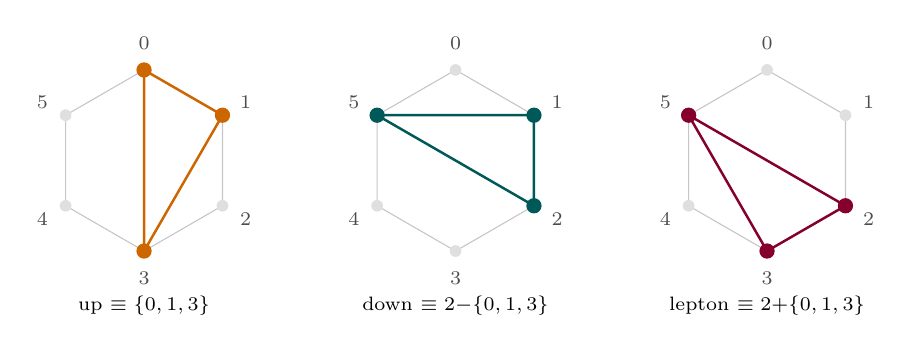
\begin{tikzpicture}[scale=0.92,>=Stealth]
 % --- up sector ---
 \begin{scope}[xshift=0cm]
   \foreach \i in {0,...,5} \coordinate (u\i) at ({90-60*\i}:1.25);
   \draw[gray!45] (u0)--(u1)--(u2)--(u3)--(u4)--(u5)--cycle;
   \foreach \i in {0,...,5} {\fill[gray!25] (u\i) circle (2.3pt); \node[font=\scriptsize,gray!60!black] at ({90-60*\i}:1.62) {\i};}
   \foreach \i in {0,1,3} \fill[orange!80!black] (u\i) circle (3pt);
   \draw[orange!80!black,line width=0.9pt] (u0)--(u1)--(u3)--cycle;
   \node[font=\scriptsize] at (0,-2.0) {up $\equiv\{0,1,3\}$};
 \end{scope}
 % --- down sector ---
 \begin{scope}[xshift=4.3cm]
   \foreach \i in {0,...,5} \coordinate (d\i) at ({90-60*\i}:1.25);
   \draw[gray!45] (d0)--(d1)--(d2)--(d3)--(d4)--(d5)--cycle;
   \foreach \i in {0,...,5} {\fill[gray!25] (d\i) circle (2.3pt); \node[font=\scriptsize,gray!60!black] at ({90-60*\i}:1.62) {\i};}
   \foreach \i in {1,2,5} \fill[teal!70!black] (d\i) circle (3pt);
   \draw[teal!70!black,line width=0.9pt] (d1)--(d2)--(d5)--cycle;
   \node[font=\scriptsize] at (0,-2.0) {down $\equiv 2{-}\{0,1,3\}$};
 \end{scope}
 % --- lepton sector ---
 \begin{scope}[xshift=8.6cm]
   \foreach \i in {0,...,5} \coordinate (e\i) at ({90-60*\i}:1.25);
   \draw[gray!45] (e0)--(e1)--(e2)--(e3)--(e4)--(e5)--cycle;
   \foreach \i in {0,...,5} {\fill[gray!25] (e\i) circle (2.3pt); \node[font=\scriptsize,gray!60!black] at ({90-60*\i}:1.62) {\i};}
   \foreach \i in {2,3,5} \fill[purple!70!black] (e\i) circle (3pt);
   \draw[purple!70!black,line width=0.9pt] (e2)--(e3)--(e5)--cycle;
   \node[font=\scriptsize] at (0,-2.0) {lepton $\equiv 2{+}\{0,1,3\}$};
 \end{scope}
\end{tikzpicture}
\caption{Flavor transport on the hexagon $C_6=Z_6=|R^+(A_3)|$. The unique distinct-distance triple
$\{0,1,3\}$ (cyclic distances $\{1,2,3\}$) and its $D_6$ orbit give the three sectors' residues mod $6$;
the total $\sum L=40=|R(D_5)|$ and the first-generation $+6$ winding come from the carrier.}
\label{fig:hexagon}
\end{figure}

\subsection{What the compiler outputs for the Standard Model and our reality}
\label{subsec:smmap}
Every entry below is an \emph{output} of $(\cthree,\gcar)$ through the $D_5\times A_3$ compiler; none is
an independent input. ``Reads'' names the lattice object the observable comes from.

\begin{center}\small
\begin{tabularx}{\linewidth}{@{}p{0.30\linewidth}p{0.40\linewidth}p{0.13\linewidth}c@{}}
\toprule
\textbf{SM / cosmology observable} & \textbf{Compiler output} & \textbf{Reads} & \textbf{St.} \\
\midrule
Number of generations & $\Nfam=3=\operatorname{rank}A_3=\dim H^1(\mathbb P^1\setminus\mu_4)$ & $A_3$ & \mE \\
Gauge algebra dimension & $\dimg=12=|R(A_3)|=\gcd(6r,2h)$ & $A_3$ & \mE \\
One generation ($16$, incl.\ $\nu^c$) & $S^+=D_5$ half-spinor $=\Lambda^{0,2,4}E$ & $D_5$ & \mE \\
Hypercharge spectrum & all $Y$ from $y_\pm=\{\tfrac12,-\tfrac13\}$; $\operatorname{Tr}X^2=120$ & $D_5$ root data & \mE \\
Abelian index $b_1$ & $10b_1=1+|\mu_4||E(K_5)|=1+4\cdot10=41$ & $\mu_4\times K_5$ & \mE \\
Fermion family occupancy & $\Oadm=\Nfam\dim S^+=(\Nfam{+}N_\Phi)|R(A_3)|=48$ & $A_3$ & \mE \\
Fine structure $\ainv=137.0359992168$ & root of $F_{U(1)}(\alpha)=0$ (explicit, unique) & EM closure & \mE \\
Cabibbo angle & $\lC=\sqrt{\useed(1-\useed)}$, $\useed=\tfrac43\cthree+48\cthree^4$ & seed & \mE \\
CKM CP phase & $\delta_{\rm CKM}=\tfrac{2\pi}{|R^+(A_3)|}+\Nfam\useed(1-\useed)=\tfrac\pi3+3\lC^2$ & $A_3^+$, seed & \mE/\mC \\
PMNS angles/phase & $\sin^2\theta_{12}=\tfrac13-\tfrac\useed2$, $\sin^2\theta_{13}=e^{-5/6}\useed$, $\delta^\nu=\tfrac{4\pi}{3}$ & $A_3^+$, seed & \mE/\mC \\
Charged-lepton hierarchy & $\det M_\ell\propto\useed^{\,h/\Nfam}=\useed^{10}$; $(5,3,2)$ & decuple & \mE/\mC \\
Mass-hierarchy transport & $\sum L=40=|R(D_5)|$; entries on $C_6=|R^+(A_3)|$ & $D_5\times A_3$ & \mE \\
Strong CP & $\theta_{\rm eff}=0$ (determinant erasure, given RP; document~3, Part~III) & --- & \mE/\mC \\
Weak CP & holonomy: $\delta_{\rm CKM}-\tfrac\pi3=\Nfam\,\useed(1-\useed)$ & $A_3^+$ & \mC \\
Gravity tree normaliser & $\xi_{\rm tree}=\tfrac{\dimg}{\dim S^+}=\tfrac34=q(A_3)$ & $A_3$ glue & \mE \\
Cosmological constant & $\rho_\Lambda/\Mbar^4=\tfrac{3}{4\pi^2}e^{2\dph}[v_{\rm geo}/(5\betarad^2\Mbar)]^{10}$ & decuple & \mE \\
Hubble anchor & $H_0\sqrt{\Omega_\Lambda}=\Mbar e^{-\ainv}/(2\pi)$ & action & \mE \\
Baryon density & $\omega_b=\lC/\AL=\lC/10$ & decuple & \mE/\mC \\
Inflation (scalaron) & $M_{\rm scal}^2/\Mbar^2=\cthree^{\,\Oadm-10b_1}=\cthree^{7}$ & deficit $r-1$ & \mE \\
Inflation amplitude & $A_s=N_\star^2\cthree^7/24\pi^2\approx2.2\times10^{-9}$ & deficit & \mC/\mO \\
\bottomrule
\end{tabularx}
\end{center}
\markerkey

\noindent\emph{Reading.} The discrete sector --- generations, gauge dimension, family content,
hypercharge, $b_1$, occupancy --- is now \emph{group-theoretic output} of $D_5\times A_3$. The
continuous sector --- $\alpha^{-1}$, $\lC$, the mixings, $\rho_\Lambda$, $H_0$, inflation --- is the
seam seed $\cthree$ and the action exponentials read on the \emph{same} carrier graphs ($K_5$ pairs,
the $C_6$ hexagon $=|R^+(A_3)|$, the decuple $\AL=\binom{\gcar}{2}=10$). What used to be a list of
separate hits is, structurally, one machine: $D_5$ carries the family and the flavor budget, $A_3$
carries the generations and the gauge dimension, $\mu_4$ glues them (and reappears as the $41$ chain,
the discriminant norms, and the CP phase step $2\pi/6$), and $\cthree$ dresses everything.

% =====================================================================
\section{Grammar I --- the carrier grammar ($3+2$)}
% =====================================================================
\noindent\emph{Machine checks for this section:} \veri{v2\_\allowbreak carrier\_\allowbreak pascal.py}


From $\gcar=5$ and the split $(b,s)=(3,2)$ the carrier data follow:
\begin{equation}
\begin{aligned}
  &\gamma_{\mathrm{car}}=\frac{\gcar}{\gcar+1}=\frac56,\quad
  \Nfam=\frac{\gcar+1}{2}=3,\quad
  \dim S^+=2^{\gcar-1}=16,\\[2pt]
  &\Oadm=\Nfam\,2^{\gcar-1}=48,\qquad
  b_1=\frac{\gcar\,2^{\gcar-2}+1}{10}=\frac{41}{10}.
\end{aligned}
\end{equation}

\subsection{Dual-root dictionary (everything from two charges)}

\par\smallskip\noindent\textbf{Two carrier roots generate the family and the transport cusps \mE.}
With $y_+=\tfrac12$ and $y_-=-\tfrac13$ (the determinant-normalised carrier eigenvalues), the full
one-family hypercharge spectrum and the flavor-transport cusps are sums of the two roots:
\[
  \begin{aligned}
  Y(Q_L)&=y_++y_-=\tfrac16, & Y(u^c)&=2y_-=-\tfrac23, & Y(d^c)&=-y_-=\tfrac13,\\
  Y(L_L)&=-y_+=-\tfrac12, & Y(e^c)&=2y_+=1, & Y(\nu^c)&=0,
  \end{aligned}
\]
\[
  \{1,\tfrac23,\tfrac13\}=\{\,2y_+,\ -2y_-,\ 2(y_++y_-)\,\},\qquad
  \gamma_{\mathrm{car}}=\operatorname{Tr}_E Y^2=3y_-^2+2y_+^2=\tfrac56,
\]
\[
  \phibase=\frac{1-\gamma_{\mathrm{car}}}{\pi}=\frac{1}{6\pi}.
\]
All residuals are exactly zero. The Standard-Model charge table is not assumed; it is built by
addition from $\{1/2,-1/3\}$.
\par\smallskip

\begin{keybox}[The $X=6Y$ quadratic and the hypercharge Pascal-sign duality \mE]
Clearing denominators with $X=6Y$ turns the two base charges into the integer roots $x_+=3$, $x_-=-2$ of
\[
  \boxed{\ x^2-x-6=0\ }:\qquad
  x_++x_-=1=N_\Phi,\quad x_+-x_-=5=\gcar,
\]
\[
  -x_+x_-=6=|R^+(A_3)|,\qquad \sqrt{\Delta}=5,
\]
so the Higgs singleton, the carrier rank and the $A_3$ hexagon all fall out of one quadratic. Counting
the signs of $X$ over a generation ($X=1^{\times6},2^{\times3},6^{\times1},(-4)^{\times3},(-3)^{\times2},0^{\times1}$)
gives the \emph{Pascal triple} again:
\[
  \boxed{\ (\#X{=}0,\,\#X{<}0,\,\#X{>}0)=(1,5,10)=\tbinom50,\tbinom51,\tbinom52\ },
\]
\[
  10{-}5{=}\gcar,\quad 5{-}1{=}|\mu_4|,\quad 10{-}1{=}\operatorname{tr}R,
\]
with $\nu^c\leftrightarrow\binom50$ the neutral singleton --- the right-handed neutrino is the Pascal zero
with a job. The moment ladder adds $\operatorname{Tr}X^2=120=5!$ and
$\operatorname{Tr}X^4/\operatorname{Tr}X^2=2280/120=19$ (an $E_8$ exponent; audit). \mE
\end{keybox}

\subsection{Carrier arithmetic (proved identities)}

The discrete coefficients are not isolated numbers; they are exact carrier traces:
\begin{align}
  10\,b_1 &= 41 = \gcar^2+(\gcar-1)^2 = \Oadm\,\gamma_{\mathrm{car}}+1
      = 1+h_{E_8}\tfrac{\dim S^+}{\dimg} = 1+30\cdot\tfrac{16}{12} = 40+1, &&\mE\\
  I_1^{\mathrm{EW}} &= \frac{41}{48}=\operatorname{Var}_{S^+}(Y)\cdot b_1=\frac{5}{24}\cdot\frac{41}{10}
      = \gamma_{\mathrm{car}}+\frac{1}{\Oadm}, &&\mE\\
  \operatorname{Tr}_{S^+}(X^2) &= 120 = 5!\quad(X=6Y), \qquad
  \dtwo = \tfrac54\dtop^2 = 2880\,\cthree^8 = 4!\cdot 5!\,\cthree^8 = 4!\,\operatorname{Tr}_{S^+}(X^2)\,\cthree^8, &&\mE\\
  \frac54 &= \underbrace{\tfrac32\cdot\tfrac56}_{B\gamma}
      = \underbrace{\tfrac{\Dstart}{\Oadm}}_{60/48}
      = \underbrace{\tfrac{\gcar}{\gcar-1}}_{5/4}
      = \frac{\dtwo}{\dtop^2}. &&\mE
\end{align}
So: $b_1$ is a Pythagorean carrier identity ($5^2+4^2$); equivalently the anchor-product form
$10b_1=p_1p_3+(\gcar-p_1)=4\cdot10+(5-4)=41$ reads ``all four glue corners times all ten carrier pairs,
plus the one leftover Higgs slot''; the electroweak exponent $41/48$ is the
hypercharge variance times the $U(1)$ budget; the second seam defect $2880\,\cthree^8$ is a product
of factorial traces $4!\cdot5!$; and the universal compression $5/4=\gcar/(\gcar-1)$ recurs whenever
the five-slot carrier projects onto four effective directions. As a minor curiosity, the SU(5)-tree
weak mixing angle rewrites as $\sin^2\theta_W^{\mathrm{tree}}=\tfrac38=\Nfam/(\gcar+\Nfam)=\Nfam/\operatorname{rank}(E_8)$
(the value is the standard one; the rewrite is a coincidence to note, not a claim). \mC

% =====================================================================
\section{Grammar II --- the seed grammar (one decoder $\useed$)}
% =====================================================================
\noindent\emph{Machine checks for this section:} \veri{v106\_\allowbreak review\_\allowbreak validation.py}


The seed is, exactly, a pure function of $\cthree$:
\begin{equation}
  \boxed{\ \useed=\varphi^{\mathrm{ret}}_0=\frac43\,\cthree+\Oadm\,\cthree^4
  =\underbrace{\frac{1}{6\pi}}_{\phibase}+\underbrace{\frac{3}{256\pi^4}}_{\dtop}=0.0531719521768\ }\qquad\mE.
\end{equation}
Its two coefficients are themselves carrier data: $\tfrac43=\dim S^+/\dimg=16/12=8/(\gcar+1)$ (so
$\phibase=1/((\gcar+1)\pi)$) and $48=\Oadm$. The seed is thus a pure function of $\cthree$ and the
carrier counts.

\par\smallskip\noindent\textbf{One seed, four readouts (and their inverses) \mE.}
\[
  \lC^2=\useed(1-\useed),\quad
  \betarad=\frac{\useed}{4\pi},\quad
  \Omega_b=\Bigl(1-\frac{1}{4\pi}\Bigr)\useed,\quad
  \sin^2\theta_{13}=e^{-5/6}\,\useed,
\]
\[
\begin{gathered}
  \useed=\frac{1-\sqrt{1-4\lC^2}}{2}=4\pi\,\betarad=\frac{\Omega_b}{1-1/(4\pi)}=e^{5/6}\sin^2\theta_{13}\\[2pt]
  =\sum_{n\ge0}C_n\,\lC^{2n+2}=\lC^2+\lC^4+2\lC^6+5\lC^8+\cdots
\end{gathered}
\]
\par\smallskip

\noindent One knob $\useed$ turns four dials simultaneously: Cabibbo mixing (the Bernoulli width
$\sqrt{\useed(1-\useed)}$), cosmic birefringence, the baryon fraction, and the reactor angle. Turning
one forces the others; there is no free per-observable tuning. The exponent $5/6$ is the carrier
trace $\gamma_{\mathrm{car}}=\operatorname{Tr}_E Y^2$, \emph{not} the Euler--Mascheroni constant
$0.5772\ldots$ (audit \mO).

% =====================================================================
\section{Grammar III --- the action grammar (exponentials of $\ainv$)}
% =====================================================================

\noindent\textbf{The relation in plain words.} The fine-structure constant is not just ``a number near
$137$'': it is the \emph{one exponential engine} behind three wildly separated scales. Take the same
$\ainv=137.036$ and divide the carrier into it: $\tfrac15$ of it sets the \emph{electroweak} scale,
$1\times$ it sets the \emph{Hubble} scale, $2\times$ it sets the \emph{cosmological constant}. The three
action charges are the Pascal row $1:5:10$ of the five-slot carrier, and the Hubble rung is just the
square root of the vacuum energy. So one constant fixes the electroweak hierarchy, dark energy and the
expansion rate at once.

\begin{center}
\begin{tikzpicture}[font=\small,
  eng/.style={rectangle,rounded corners=3pt,draw=tfgold!80!black,fill=tfgold!16,line width=1pt,align=center,inner sep=6pt},
  sc/.style={rectangle,rounded corners=2pt,draw=tfgreen!70!black,fill=tfgreen!8,align=center,inner sep=4pt,text width=46mm},
  ar/.style={-{Stealth[length=2.6mm]},thick,tfgray}]
  \node[eng] (e) at (0,0) {\textbf{one engine}\\$\ainv=137.0359992$};
  \node[sc] (ew) at (6.2,2.0) {\textbf{electroweak} \;($q{=}\tfrac1{\gcar}$)\\$v_{\rm EW}/\Mbar\sim e^{-\ainv/5}$};
  \node[sc] (h)  at (6.2,0.0) {\textbf{Hubble} \;($q{=}1$)\\$H_0/\Mbar\sim e^{-\ainv}=\sqrt{\rho_\Lambda}$};
  \node[sc] (l)  at (6.2,-2.0){\textbf{cosm.\ constant} \;($q{=}2$)\\$\rho_\Lambda/\Mbar^4\sim e^{-2\ainv}$};
  \draw[ar] (e) to[bend left=12] node[above,font=\scriptsize]{$\div\,5$} (ew);
  \draw[ar] (e) -- node[above,font=\scriptsize]{$\times\,1$} (h);
  \draw[ar] (e) to[bend right=12] node[below,font=\scriptsize]{$\times\,2$} (l);
  \node[font=\scriptsize,tfgray,align=center] at (3.0,-3.25)
    {action charges $1:\gcar:2\gcar=1:5:10=\binom50:\binom51:\binom52$ (Pascal row of $K_5$)};
\end{tikzpicture}
\end{center}

Read every dimensionless ratio through its \emph{action} and ask for the action charge:
\begin{equation}
  \boxed{\ x=R_x\,e^{-A_x},\qquad A_x=q_x\,\ainv+\Delta_x,\qquad q_x\in\Bigl\{\tfrac{1}{\gcar},\,1,\,2\Bigr\}.\ }
\end{equation}
The robust ladder and its residues are
\begin{center}\small
\begin{tabular}{@{}lllll@{}}
\toprule
sector & action $A_x$ & charge $q_x$ & residue $R_x$ & value of $-\ln x$ \\
\midrule
electroweak $v_{\mathrm{geo}}/\Mbar$ & $(\ainv+\dph)/\gcar$ & $1/\gcar$ & $\gcar\betarad^2$ & $36.85$ \\
Hubble $H_0/\Mbar$ & $\ainv$ & $1$ & $1/(2\pi\sqrt{\Omega_\Lambda})$ & $138.68$ \\
cosm.\ const.\ $\rho_\Lambda/\Mbar^4$ & $2\ainv$ & $2$ & $3/(4\pi^2)$ & $276.65$ \\
\bottomrule
\end{tabular}
\end{center}
\begin{equation}
  \AEW=\frac{\ainv+\dph}{\gcar}=27.5259,\qquad \AL=2\ainv=274.072,\qquad
  \boxed{\ \AEW{:}\AH{:}\AL=1{:}5{:}10\ }.
\end{equation}
The leading ratio is exact: $\AL/(\ainv/\gcar)=2\gcar=10$ (with the transport correction
$\AL/\AEW=9.957$). The claim is that the \emph{action charges}, not the raw logarithms, form the
ladder.

\begin{figure}[ht]
\centering
\includegraphics[width=0.82\linewidth]{figures/action_tower.pdf}
\caption{Action tower (data plot, \texttt{verification/make\_figures.py}). The three action charges
$A_x=-\ln x$ for the electroweak, Hubble and cosmological-constant ratios fall on the line
$A=(\ainv/5)\binom5k$: one engine $\ainv$ generates all three scales with the Pascal exponents $1:5:10$.}
\label{fig:actiontower}
\end{figure}

\subsection{The EM closure: $\ainv$ as an explicit fixed point (made explicit here)}
The engine $\ainv$ is not an input --- it is the unique root of an explicit closure equation
(the exact electromagnetic closure theorem). With $\cthree=1/(8\pi)$, $\phibase=1/(6\pi)$,
$q(\alpha)=\dtop e^{-2\alpha}$ and the seam response $\phiseam(\alpha)=\phibase+q(\alpha)(1-q(\alpha))^{-5/4}$,
\begin{equation}
  \boxed{\ F_{U(1)}(\alpha)=\alpha^3-2\cthree^3\alpha^2-\tfrac{4}{5}\cthree^6\Bigl(\textstyle\sum_{f,j}L_{f,j}+N_\Phi\Bigr)\log\frac{1}{\phiseam(\alpha)}=0\ }\qquad\mE/\mC ,
\end{equation}
where the coefficient is $\tfrac45(\sum L+N_\Phi)\cthree^6=\tfrac45\cdot41\,\cthree^6=8b_1\cthree^6$, so the
fine-structure constant reads the \emph{flavor transport budget} $\sum L=40$ and the $U(1)$ index
$b_1=41/10$.

\begin{lemma}[Existence and uniqueness of the EM fixed point]
\label{lem:emclosure}
$F_{U(1)}$ has \emph{exactly one} positive root, and it is simple.
\end{lemma}
\begin{proof}
Write $F_{U(1)}(\alpha)=h(\alpha)-C\,g(\alpha)$ with $h(\alpha)=\alpha^3-2\cthree^3\alpha^2$,
$C=\tfrac45\cthree^6M>0$ ($M=41$), and $g(\alpha)=-\log\phiseam(\alpha)$. Since
$q(\alpha)=\dtop e^{-2\alpha}\in(0,1)$ is strictly decreasing, $\phiseam=\phibase+q(1-q)^{-5/4}$ is $C^1$
and decreasing, so $g$ is $C^1$, bounded, and slowly increasing with $g'(\alpha)=O(q)$ tiny; numerically
$g\in[2.9342,2.9343]$ on the admissible window. The cubic $h$ has its interior critical point at
$\alpha_c=\tfrac43\cthree^3=8.399\times10^{-5}$, with $h(0)=0$ and $h<0$ on $(0,\alpha_c)$.
\emph{Monotonicity (corrected endpoint).} Since
$F_{U(1)}'(\alpha)=3\alpha^2-4\cthree^3\alpha-C\,g'(\alpha)$ and at $\alpha_c$ the first two terms
\emph{cancel} ($3\alpha_c=4\cthree^3$), one has $F_{U(1)}'(\alpha_c)=-C\,g'(\alpha_c)\approx-5.89\times10^{-10}<0$:
the derivative is \emph{not} yet positive at $\alpha_c$. Its first zero lies slightly above, at
$\alpha_0=8.6264\times10^{-5}$ (where $3\alpha_0^2-4\cthree^3\alpha_0=C\,g'(\alpha_0)$), with $F_{U(1)}'<0$ on
$(\alpha_c,\alpha_0)$ and $F_{U(1)}'>0$ on $(\alpha_0,\infty)$. Now $F_{U(1)}(0)=-C\,g(0)<0$, and
$F_{U(1)}$ \emph{decreases} on $(0,\alpha_0]$ (both $h$ and $-Cg$ decrease on $(0,\alpha_c]$, then $F_{U(1)}'<0$
on $[\alpha_c,\alpha_0]$), so $F_{U(1)}(\alpha_0)\approx-3.82\times10^{-7}<0$; thereafter $F_{U(1)}$ is strictly
increasing to $+\infty$. Hence $F_{U(1)}<0$ on $(0,\alpha_0]$ and strictly increasing on $[\alpha_0,\infty)$, so
it crosses zero \emph{exactly once}. The crossing has $F_{U(1)}'(\alpha_\star)=1.58\times10^{-4}>0$, so the
root is simple. A sign scan on $(0,0.05)$ confirms a single change. \emph{Rigorous version:} an
\textbf{interval-arithmetic} enclosure (\texttt{mpmath.iv}) brackets the root in
$[0.00729735256220970,\,0.00729735256221000]$ with $F_{U(1)}<0$ on the lower and $>0$ on the upper
endpoint (definite signs), and a $200$-cell interval partition of $(\alpha_c,0.05)$ contains exactly
\emph{one} indeterminate (root-bearing) band --- a verified uniqueness, not merely a sampled one.
\veri{v3\_em\_alpha.py}
\end{proof}

\noindent Solving:
\begin{equation}
  \boxed{\ \alpha_\star=0.00729735256220985\ldots,\quad \ainv=137.0359992168407\ldots\ }\quad\mE
\end{equation}
\veri{v3\_em\_alpha.py}\;
versus CODATA-2022 $\ainv=137.035999177(21)$ --- a relative deviation $2.9\times10^{-10}$ ($\approx1.9\sigma$
on the tiny experimental error; the older 2018 value $137.035999084$ gave $9.7\times10^{-10}$, so the
agreement \emph{improved} in relative terms). The exponent $-5/4$ in $\phiseam$ is the carrier
discriminant norm $q(D_5)$, and $\dtop=48\cthree^4$, so the closure is built only from $\cthree$, the
carrier, and the flavor budget. This discharges the former open audit point: the EM closure is a stated,
existence-/uniqueness-proven, numerically reproduced equation, not a fit.

\par\smallskip\noindent\textbf{Why \emph{this} function: the boundary $U(1)$ Ward reading (Theorem C) \mE/\mC.}
$F_{U(1)}$ is not a chosen ansatz but the reduced Ward identity of the boundary $U(1)$ partition function
$Z_{\partial}=Z_{\mathrm{Maxwell}}\,Z_{\mathrm{Calder\acute on}}\,Z_{\mathrm{transport}}$, with three terms
whose coefficients are compiler atoms, not fits:
\[
  \underbrace{\alpha^3}_{\text{Maxwell moment}}\;
  \underbrace{-\,2\cthree^3\alpha^2}_{\text{Calder\'on sheet}\,(2=|\Z_2|)}\;
  \underbrace{-\,8b_1\cthree^6\log\tfrac1{\phiseam}}_{\text{$C_6$ transport det.}}=0,\qquad
  8b_1=\tfrac45 M=\tfrac45(\textstyle\sum L+N_\Phi)=\tfrac{164}{5}.
\]
The Calder\'on factor $2=|\Z_2|$ (sheet), the transport power $\cthree^6$ is the $C_6$ hexagon, and the
seam exponent $-\tfrac54=-q(D_5)$ is the carrier discriminant norm. \textbf{Typing:} the three-term
decomposition and the coefficient identities ($8b_1=\tfrac45 M$, $-\tfrac54=q(D_5)$) are exact \mE; the
\emph{physical origin} as a boundary Ward closure (the lemmas $\partial_\tau\log Z_{\mathrm{Maxwell}}=\alpha^3$,
$\partial_\tau\log Z_{\mathrm{Calder\acute on}}=-2\cthree^3\alpha^2$, $\partial_\tau\log\det\nolimits_\zeta(1-\mathcal T_{C_6,U(1)})=-8b_1\cthree^6\log\tfrac1{\phiseam}$)
is a conjectured \mC\ interpretation, not yet machine-proven. \veri{v48\_em\_ward.py}
\par\smallskip
\noindent\textbf{The determinant-line (Quillen) form.} (\veri{v341\_alpha\_quillen.py})
The three terms assemble into a single \emph{stationarity} statement for the boundary $U(1)$ determinant line,
\[
  \underbrace{\bigl[\alpha^3-2\cthree^3\alpha^2\bigr]}_{\delta\log\det\Delta_{U(1)}}
  \;=\;\underbrace{\bigl[8b_1\cthree^6\bigr]}_{\text{ctr.}}\;
  \underbrace{\bigl[\log\tfrac1{\phiseam}\bigr]}_{\text{seam resp.}},
\]
so $F_{U(1)}=0$ is $\delta\log\det\Delta_{U(1)}+\text{counterterm}+\text{seam response}=0$. Every factor is a
\emph{named} object, not a knob: the counterterm coefficient is $8b_1\cthree^6=(\operatorname{rank}E_8)\,b_1\,\cthree^6$
(index $\times$ heat-kernel), $\cthree=1/(8\pi)$ is the Gauss--Bonnet boundary coefficient, the exponent
$-\tfrac54=-q(D_5)$ is one carrier discriminant norm and the seam base $\phibase=1/(6\pi)=\tfrac43\cthree$ carries
the \emph{other}, $\cthree/\phibase=\tfrac34=q(A_3)$ --- both glue forms appear, and the split is verified at the
root. \textbf{Typing (and: no new gate).} The determinant-line assembly and all coefficient identities are exact
\mE; $\ainv$ itself stays closed \mE\ (unique root $+$ ablation). This adds \emph{no} open item --- it
\emph{sharpens} the pre-existing \mO/physical-origin obligation \texttt{EM.WARD.01} (the ``why \emph{this}
function'' residual, already conjectural) by naming every coefficient. The one still-open part \emph{is} that
residual, now \emph{named} as its own tracked target \texttt{ALPHA.QUILLEN.EXACT.01}
(\veri{v382\_alpha\_quillen\_exact.py}): the from-first-principles AQFT/$\zeta$ proof that
$\delta_\tau(\log\det\nolimits_\zeta\Delta_{U(1)}+8b_1\cthree^6\log\varphi_{\mathrm{seam}})=0$ --- i.e.\ that
$F_{U(1)}$ is the \emph{exact} Quillen functional of the seam $U(1)$, the variational principle \emph{derived}, not
assembled. It is a \emph{face} of \texttt{SEAM.EQUIV.01} (\vref{v336}) --- the seam $U(1)$ determinant line lives on
the same holomorphic net, so once the net is $(E_8)_1$ its $U(1)$ sub-determinant is fixed --- hence no second
independent gate, just the sharpest remaining EM-Ward obligation, now citable on its own.
\emph{Honest progress towards it (\veri{v391\_alpha\_quillen\_progress.py}), without closing it:} a solvable
model $\det_\zeta(-\partial_\tau^2{+}m^2)$ on a circle $=(2\sinh(\beta m/2))^2$ has the closed $m$-variation
$\beta\coth(\beta m/2)=2/m+(\beta^2/6)m-(\beta^4/360)m^3+\dots$, a heat-kernel/Laurent series --- so a
$\zeta$-determinant's variation is \emph{structured} heat-kernel data, and the counterterm $8b_1\cthree^6$ (a
Gauss--Bonnet heat-kernel power) is the right \emph{kind} of object. This \emph{reduces}
\texttt{ALPHA.QUILLEN.EXACT.01} to the named sub-target ``the seam $U(1)$ Seeley--DeWitt coefficient $=8b_1\cthree^6$'',
but the target itself stays \mO\ (an external math proof, \vref{v384}); the value $\ainv$ stays \mE.
\emph{A second honest step (\veri{v433\_alpha\_quillen\_heatkernel.py}) bridges this reduction to the heat-kernel
origin below, without closing it:} v391's circle reached only the low orders $a_0,a_1$, whereas a solvable \emph{4D}
model --- the flat $\Delta=-\partial^2{+}m^2$ on $T^4$, $\operatorname{Tr}e^{-t\Delta}=V/(4\pi)^2\,t^{-2}e^{-tm^2}$
--- has $a_4=Vm^4/(2(4\pi)^2)\neq0$, \emph{reaching} the $t^0$ (conformal-anomaly) order the circle could not, the
very order in which the quadratic term is grounded below (\vref{v342}, Gilkey $a_4$). So a $\zeta$-determinant's
variation is heat-kernel data \emph{at the $a_4$ order}, and the measure itself is $\cthree$-built,
$(4\pi)^{-2}=(2\cthree)^2=4\cthree^2$; the \emph{actual} seam $a_4=8b_1\cthree^6$ and the cubic $\alpha^3$ Chern
moment stay \mO\ (\vref{v384}), the seam $F$-normalisation \mC\ (retyped by the fifth step below,
\vref{v470}, as the embedding index $k_Y{=}5/3$).
\par\smallskip
\noindent\textbf{The heat-kernel origin of the terms (\veri{v342\_em\_ward\_heatkernel.py}).} The determinant-line
form is more than bookkeeping: its terms are textbook heat-kernel coefficients. \mE\ $\cthree=1/(8\pi)$ \emph{is}
the boundary Gauss--Bonnet coefficient ($\oint_{S^2}K=2\pi\chi=4\pi$, $\cthree=1/(|\Z_2|\oint K)$, the same
$\chi{=}2$ as the marks, \vref{v216}). \mE\ the $\alpha^2$ (Calder\'on) term \emph{is} the Gilkey gauge-curvature
coefficient: the $U(1)$ Laplacian's Seeley--DeWitt $a_4$ contains $30\,\Omega_{ij}\Omega^{ij}/360=\tfrac1{12}\Omega^2$
(Gilkey, \emph{Invariance Theory}, Thm 4.8.16), and with $\Omega=i\alpha F$ this forces an $-(\alpha^2/12)F^2$
contribution to $\log\det\Delta_{U(1)}$ --- so the Calder\'on $-2\cthree^3\alpha^2$ is the gauge-curvature
(Quillen-curvature) piece, not an ansatz. \mE\ the $\cthree$-orders $\{0,3,6\}$ are an arithmetic ladder (step $3=$
the three channels; $6=|R^+(A_3)|$, the $C_6$ hexagon), and the $\pi$-power test confirms it: $2\cthree^3=1/(256\pi^3)$
carries $\pi^3$, i.e.\ \emph{three} boundary $\cthree$-insertions, not a single bulk coefficient. \textbf{Typing:} the
boundary structure and the gauge-curvature origin of the quadratic term are heat-kernel-forced \mE; the exact
coefficient value is \mC\ (the seam $F$-normalisation --- retyped as the embedding index $k_Y{=}5/3$ by the
fifth step below, \vref{v470}); the cubic $\alpha^3$ Maxwell moment (a topological/Chern
level) and the full ``this \emph{is} the seam $U(1)$ $\zeta$-determinant'' claim stay \mO\ --- exactly the
\texttt{EM.WARD.01} residual, unchanged. So the quadratic/curvature half of the EM-Ward origin is now derived; the
cubic-moment half remains the honest open part.
\emph{A third honest step (\veri{v434\_alpha\_quillen\_betafunction.py}) settles those residuals and shows they are
not three independent problems.} The counterterm's \emph{matter} factor is heat-kernel-forced too: by the
$\beta=a_4$ theorem the one-loop $U(1)_Y$ $\beta$ \emph{is} the $a_4$ coefficient, and the carrier hypercharge
content gives $\sum\tfrac23 Y_f^2+\tfrac13 Y_s^2=41/6$ (SM) $\Rightarrow b_1=41/10$ (GUT, \vref{v159}/\vref{v246}),
so $8b_1\cthree^6=b_1\,(\operatorname{rank}E_8)\,\cthree^6$ is an $a_4$ content coefficient times a boundary
geometry --- the same \emph{kind} of object as the Calder\'on $a_4$. The exact value then turns only on the seam
$F$-normalisation, so the ``actual seam $a_4$'' residual \emph{is} the $F$-normalisation \mC\ (one obligation, not
two); and the cubic factors $a^3-2\cthree^3 a^2=a^2(a-2\cthree^3)$, exhibiting $a^3$ as the first moment of the
Chern density $a^2$ --- a level whose from-first-principles origin stays \mO. The EM-Ward residual is thus
\emph{one} \mC\ $+$ \emph{one} \mO, not three.
\emph{A fourth honest step (\veri{v435\_alpha\_quillen\_chernlevel.py}) sharpens that single remaining \mO\
--- residual (2), the cubic $\alpha^3$ Chern level --- without closing it.} A $\pi$-power / metric-independence
test partitions the closure: the three coefficients carry $\pi$-powers exactly $\{0,3,6\}$ ($k_0=1$;
$-2\cthree^3=-1/(256\pi^3)$; $-8b_1\cthree^6=-41/(327680\pi^6)$), so the Maxwell $a^3$ is the \emph{unique}
$\pi^0/\cthree^0$ (metric-\emph{independent}) term. A heat-kernel boundary coefficient always carries the
$(4\pi)^{-d/2}$ measure; a metric-independent term carries none --- the signature of a \emph{topological}
term. So the test confirms, now from a test rather than a claim, that $a^3$ is a level and not a
Seeley--DeWitt curvature integral (the other two terms are heat-kernel boundary data). \mE\ \emph{Conditional}
on the Chern--Simons/$\eta$ reading of the Maxwell moment (the \texttt{EM1} interpretation, \vref{v48}),
large-gauge invariance quantises the seam $U(1)$ level to $\Z$, so $k_0=1$ is the \emph{unit} (minimal) level
--- an integer, not a tunable real. \mC\ What stays \mO\ is the \texttt{EM1} lemma itself --- the
from-first-principles Chern--Simons-boundary proof that $\partial_\tau\log Z_{\mathrm{Maxwell}}=a^3$ ---
external math (type A, \vref{v384}).
\emph{A fifth honest step (\veri{v470\_alpha\_inflow\_level.py}) upgrades both leftovers, still without
closing the target.} \mC\ \emph{The level is computed, not minimal:} under the same \texttt{EM1} reading, the
$a^3$ coefficient $k_0=1$ \emph{equals} the FHS bulk Chern invariant $|C|=1$ of the very p$+$ip collar that
realises S3 of \texttt{SEAM.EQUIV.01} (\vref{v367}/\vref{v461}; control $C(M{=}3)=0$) --- ``why exactly
$1$'' is answered by a computation plus the cited inflow identification (TKNN / Avron--Seiler--Simon
quantisation; Callan--Harvey inflow; the APS/Witten $\eta{=}$CS reading of $\delta\log\det$;
Quillen/Bismut--Freed determinant-line integrality), \emph{replacing} the minimality assumption of the fourth
step. \mE\ \emph{The $F$-normalisation is the embedding index:} $k_Y=\operatorname{tr}_{\bar 5}(Y^2)/
\operatorname{tr}(T_3^2)=(5/6)/(1/2)=5/3$ (Ginsparg 1987), so $(3/5)\times\tfrac{41}{6}=\tfrac{41}{10}=b_1$
exactly --- the ``GUT $3/5$'' \emph{is} the inverse embedding index, and once the seam net is $(E_8)_1$ at
level $1$ the $U(1)_Y$ normalisation $\langle J(z)J(w)\rangle=k/(z{-}w)^2$ is \emph{fixed} by it (level-$1$
current-algebra rigidity, no continuous dial): the seam $F$-normalisation \mC\ has \emph{zero independent
content} --- a face of \texttt{SEAM.EQUIV.01}, per the \vref{v382} typing. \mC\ \emph{One phase, two
responses:} the collar phase carries $c_-=8$ (gravitational, feeding \texttt{SEAM.EQUIV.01}/S3, \vref{v456})
\emph{and} $C=1$ ($U(1)$, feeding \texttt{EM1}) --- so discharging the one realisation input feeds both named
targets at once.
\emph{A sixth honest step (\veri{v472\_quillen\_detline\_moduli.py}) exhibits that bridge lemma at the finite
level.} \texttt{ALPHA.QUILLEN.EXACT.01} names the level as the curvature of the \emph{determinant line over
the $U(1)$ moduli} (Quillen/Bismut--Freed curvature, Dai--Freed section) --- and the fifth step computed the
Chern invariant only over the Bloch Brillouin zone, the translation-invariant shortcut. The sixth step
computes the Quillen-shaped object itself: the same collar Hamiltonian in real space with twisted boundary
conditions --- the twist torus $(\theta_x,\theta_y)$ \emph{is} the moduli space of flat $U(1)$ connections
--- and the Fukui--Hatsugai--Suzuki curvature of the determinant line of the occupied frame over that torus
integrates to $2\pi\cdot 1$ exactly ($10^{-9}$), size-independently ($L=4,6$), with clean controls (trivial
collar $\to 0$, orientation flip $\to -1$), the twist-moduli integer equal to the Bloch-BZ integer for all
three phases (Niu--Thouless--Wu), and the Fermi gap open over the whole torus (the Dai--Freed section has no
zero). So ``$\delta\log\det(\mathrm{seam~model})=$ the inflow response'' \emph{holds verbatim at the
finite/model level}, where $\log\det$ of the occupied frame replaces $\log\det_\zeta$. \mE\ (computation) /
\mC\ (the EM1 reading). What stays \mO\ is the \emph{continuum} identification
``$\delta\log\det_\zeta(\mathrm{seam})=$ the inflow response'' on the abstract seam (the
\texttt{SEAM.EQUIV.01} face); \texttt{ALPHA.QUILLEN.EXACT.01} stays \mO, and $\ainv$ stays \mE\ regardless.
\emph{A seventh step unifies this target with the $\phiz$-puncture target
(\veri{v484\_seam\_contact\_unit.py}).} The $\{0,3,6\}$ $\cthree$-ladder above and the puncture's per-mark
weight $\cthree$ (\vref{v483}) are \emph{one} rule --- the seam contact unit --- and it is not a new
unknown: ``$\cthree$ per insertion'' \emph{is} the KMS seam unit $2\pi=1/(4\cthree)$ with
$\tfrac14=1/|\mu_4|$ (\vref{v239}), i.e.\ one bare boundary propagator ($\tfrac1{2\pi}=4\cthree$)
orbit-averaged over the four marks. \mE\ derived on the seam circle for the finite cycle sector (the bare
Green function takes integer multiples of $\cthree\ln2$ at the $\mu_4$ separations; the log-det contact
expansion is exactly graded in $\cthree$ per insertion), with the grammar already suite-wide (the
$\Lambda$ prefactor $\tfrac{3}{4\pi^2}=48\cthree^2$, \vref{v60}, carries the same $\Omega_{\mathrm{adm}}=48$
at two insertions). \mC/\mO\ Consequence: \texttt{ALPHA.QUILLEN.EXACT.01} and \texttt{HYP.PHI0.PUNCTURE.01}
\emph{merge} into one remaining analytic step --- the diagonal zeta-renormalisation at the marks plus the
state-multiplicity matching ($41=10b_1$ here, $48=\Omega_{\mathrm{adm}}$ there).
\emph{An eighth step settles that remaining step at the computable level
(\veri{v485\_contact\_diagonal\_closed.py}).} \mE\ The renormalised coincident-point Green function on a
circle of circumference $\ell$ is $G_{\mathrm{reg}}(0;\ell)=\tfrac1\pi\ln(\ell/2\pi)$ exactly --- it
\emph{vanishes} precisely at $\ell=2\pi=1/(4\cthree)$, the KMS seam circumference (\vref{v239}): the seam
scale is the unique zero-self-energy scheme point, and the log is the pure \emph{scale} channel (matching
the fact that $F_{U(1)}$ carries exactly \emph{one} log term while the $\phiz$ split is log-free). \mE\
With the diagonal zero the mark contact calculus \emph{resums in closed form} (the BFK/gluing route,
\vref{v151}): $\det(I-uC)=(1-4u)(1+2u)^2$ with $u=\varepsilon\cthree\ln2$ --- all orders, the linear term
absent because $\operatorname{Tr}C=0$. \mE\ And the two multiplicities are \emph{one} state set under two
response weights: the same $48=3\times16$ admissible states counted flat give the $\phiz$ puncture count
$48=\Omega_{\mathrm{adm}}$, and $Y^2$/loop/GUT-weighted give the alpha budget $41=10b_1=40+1$
($\operatorname{Tr}_{16}Y^2=\tfrac{10}3$ exact, $\nu^c=0$; Ginsparg, \vref{v470}). \mC/\mO\ Net: every
finite/computable piece of the merged target is proven; the single remaining \mO\ is the identification of
the abstract seam $\zeta$-det with this glued mark determinant --- \emph{exactly} the \vref{v382} typing
(a face of \texttt{SEAM.EQUIV.01}), now substantiated computationally rather than asserted.
\par\smallskip

\noindent The full ablation --- which inputs are load-bearing and which only set the last digit --- is in
the \hyperref[sec:ablation]{Ablation appendix} below.

\emph{Inversion test (this round).} Running the closure backwards --- inserting the \emph{measured}
$\alpha$ and solving for the integer budget $M=\sum L+N_\Phi$ --- returns
$M=41.0000001\ldots$, i.e.\ the external measurement reconstructs the internal discrete budget
$41=40+1$ to $10^{-7}$. This is stronger than ``we hit $\alpha$'': the equation reads the discrete
$41$ out of nature. \mE

\subsection{The decuple bridge (new, exact headline)}

Eliminating $\ainv=\gcar\,\AEW-\dph$ between the electroweak and the cosmological-constant lines
gives a direct relation between the two scales:

\begin{keybox}[Decuple bridge: $\Lambda$ is the tenth power of the stripped EW scale \mE]
\begin{equation}
  \boxed{\ \frac{\rho_\Lambda}{\Mbar^4}
  =\frac{3}{4\pi^2}\,e^{2\dph}\,
  \left[\frac{v_{\mathrm{geo}}}{5\,\betarad^2\,\Mbar}\right]^{10}\ }
\end{equation}
where the exponent $10=2\gcar$ and $5=\gcar$. Verified to a relative residual $\sim10^{-159}$.
\end{keybox}

\noindent\emph{Proof.} From $v_{\mathrm{geo}}/\Mbar=\gcar\betarad^2 e^{-\AEW}$,
$e^{-\AEW}=(v_{\mathrm{geo}}/\Mbar)/(\gcar\betarad^2)$. From
$\rho_\Lambda/\Mbar^4=\tfrac{3}{4\pi^2}e^{-2\ainv}$ and $\ainv=\gcar\AEW-\dph$,
$e^{-2\ainv}=e^{2\dph}e^{-2\gcar\AEW}=e^{2\dph}(e^{-\AEW})^{2\gcar}$. Substituting and using
$2\gcar=10$, $\gcar=5$ gives the boxed form. $\square$

\smallskip
In words: the electroweak scale is not directly the $\Lambda$ scale, but once the electroweak ratio
is stripped of its small $\betarad$ prefactor, $\Lambda$ is its tenth power, and the ``ten'' is
$2\gcar$, not a fitted exponent. This is the direct algebraic compression of the action ladder.

\subsection{The full power tower: $x^{1},x^{5},x^{10}$ on the carrier graph $K_5$}

The decuple bridge is one rung of a tower. Writing $x:=e^{-\AEW}=v_{\mathrm{geo}}/(5\betarad^2\Mbar)$
for the stripped electroweak unit, all three cosmological scales are powers of the \emph{same} $x$
with binomial exponents (verified exactly):
\begin{equation}
  \boxed{\ \frac{v_{\mathrm{geo}}}{5\betarad^2\Mbar}=x^{\binom50}=x,\qquad
  \frac{H_0}{\Mbar}=x^{\binom51}R_{\mathrm H}=x^5R_{\mathrm H},\qquad
  \frac{\rho_\Lambda}{\Mbar^4}=x^{\binom52}R_\Lambda=x^{10}R_\Lambda\ }
\end{equation}
with residues $R_{\mathrm H}=e^{\dph}/(2\pi\sqrt{\Omega_\Lambda})$ and $R_\Lambda=\tfrac{3}{4\pi^2}e^{2\dph}$.
\mE. The exponents are the complete-graph counts of the five-slot carrier $K_5$:
\[
  H \leftrightarrow \text{vertices of }K_5\ (\,\#=\tbinom51=5\,),\qquad
  \Lambda \leftrightarrow \text{edges of }K_5\ (\,\#=\tbinom52=10\,).
\]
So the cosmological constant is the product of one stripped-electroweak unit over every carrier
\emph{pair} ($K_5$ edge product), and the Hubble scale the product over every carrier \emph{slot}
($K_5$ vertex product). This is the cleanest single-variable statement of the action ladder.

\subsection{Hubble is the square root of $\Lambda$ (corollary, exact)}

On the comparison layer $\rho_\Lambda/\Mbar^4=3\Omega_\Lambda(H_0/\Mbar)^2$; equating to the TFPT
line gives
\begin{equation}
  \boxed{\ \frac{H_0}{\Mbar}=\frac{e^{-\ainv}}{2\pi\sqrt{\Omega_\Lambda}}\ },\qquad
  \AH=-\ln\frac{H_0}{\Mbar}=\ainv+\ln\!\bigl(2\pi\sqrt{\Omega_\Lambda}\bigr)=138.68 .
\end{equation}
So the Hubble rung is \emph{not} an independent third hit: it is the square root of the vacuum
energy plus a geometric cosmology factor. The genuine TFPT content is the single $e^{-\ainv}$.
(The numerical coincidence $\AH-\ainv\approx\pi^2/6$ is just $\ln(2\pi\sqrt{\Omega_\Lambda})$ and is
$\Omega_\Lambda$-dependent; not a claim. \mO)

\subsection{The $\sim123$ orders of the cosmological constant}
\begin{equation}
  \log_{10}\frac{\MPl^4}{\LamIR}
  =\underbrace{\frac{2\ainv}{\ln10}}_{119.028}+\underbrace{\log_{10}\frac{1}{\dtop}}_{3.920}
  =122.948\approx123 .
\end{equation}
The ``$119$'' is the action $2\ainv$; the ``$\approx4$'' is the seam defect $\dtop=\Oadm\cthree^4$.

\begin{winbox}[High-precision cosmological constant: a $\sim10^{-13}$ prediction \mE]
Because $\ainv$ is a \emph{derived} number (the EM fixed point, known to $13$ digits) and the residue
$3/(4\pi^2)$ is exact, the dimensionless vacuum energy is predicted essentially exactly:
\begin{equation}
  \boxed{\ \frac{\rho_\Lambda}{\Mbar^4}=\frac{3}{4\pi^2}\,e^{-2\ainv}=7.12533\times10^{-121}\ }\qquad\mE\ \veri{v7\_gravity\_cosmo.py} ,
\end{equation}
i.e.\ a dark-energy scale
$\rho_\Lambda^{1/4}=\bigl(\tfrac{3}{4\pi^2}\bigr)^{1/4}\Mbar\,e^{-\ainv/2}=2.23747\ \mathrm{meV}$
(reduced Planck mass $\Mbar=2.435323\times10^{18}$ GeV). The \emph{dimensionless} ratio carries no
observational input --- its uncertainty is that of $\ainv$, $\sim10^{-13}$ relative; the absolute
$\mathrm{meV}$ value inherits only the Planck-mass uncertainty ($\sim2\times10^{-5}$). Both are
\emph{far} sharper than the measured vacuum energy (Planck $\rho_\Lambda^{1/4}\simeq2.24$ meV, known to
$\sim1\%$ and entangled with the $H_0$ tension). So TFPT pins the cosmological constant several orders of
magnitude more precisely than it is currently measured --- a genuine, falsifiable forward prediction:
any future sub-percent $\rho_\Lambda$ must land on $2.2375$ meV.
\end{winbox}

\subsection{The ladder is binomial; $2\gcar=\binom{\gcar}{2}$ singles out $\gcar=5$}

In units of the electroweak action $\ainv/\gcar$, the three rungs are the first three binomial
coefficients of the five-slot carrier:
\begin{equation}
  \frac{\AEW}{\ainv/\gcar}:\frac{\AH}{\ainv/\gcar}:\frac{\AL}{\ainv/\gcar}
  =1:\gcar:2\gcar
  =\binom{\gcar}{0}:\binom{\gcar}{1}:\binom{\gcar}{2}
  =1:5:10 .
\end{equation}
The first two are automatic ($\binom{\gcar}{0}=1$, $\binom{\gcar}{1}=\gcar$). The non-trivial content
is the cosmological-constant charge:
\begin{equation}
  \boxed{\ 2\gcar=\binom{\gcar}{2}\quad\Longleftrightarrow\quad \gcar=5\ }\qquad\mE\ \veri{v2\_carrier\_pascal.py},
\end{equation}
since $\binom{\gcar}{2}=\tfrac{\gcar(\gcar-1)}{2}=2\gcar\iff\gcar=5$. So the ``double overlap'' charge
$2\gcar$ equals the number of carrier-slot \emph{pairs} $\binom{\gcar}{2}$ \emph{only} at $\gcar=5$:
the cosmological constant is suppressed by one action unit per carrier pair, and this combinatorial
reading is exclusive to the physical rank. It is an independent overdetermination of $\gcar=5$ from
the action grammar (cf.\ the landscape section).

\subsection{Discriminant action theorem: the ladder reads the hypercharge discriminant}

The $\gcar$ in the action ladder is not merely a rank: it is the square root of the discriminant of
the carrier (hypercharge) polynomial. For a general split $b+s=g$ the carrier polynomial is
$bs\,Y^2+(s-b)Y-1=0$ with discriminant
\begin{equation}
  \Delta_Y=(s-b)^2+4bs=(b+s)^2=\gcar^2,\qquad\text{so for }6Y^2-Y-1=0:\ \Delta_Y=25,\ \sqrt{\Delta_Y}=5=\gcar .
\end{equation}
Hence the action ladder is, exactly,
\begin{equation}
  \boxed{\ \AEW=\frac{\ainv}{\sqrt{\Delta_Y}},\qquad \AH=\sqrt{\Delta_Y}\,\AEW,\qquad
  \AL=\binom{\sqrt{\Delta_Y}}{2}\AEW\ }\qquad\mE .
\end{equation}
The electroweak hierarchy therefore reads the \emph{discriminant of the hypercharge polynomial}, tying
the Standard-Model hypercharge derivation directly to the EW-hierarchy and $\Lambda$ problems.

\subsection{A two-dimensional action lattice}

All scales sit on the integer lattice spanned by two generators --- the gauge unit $\ainv/\gcar$ and
the flavor unit $L_0=\ln(1/\useed)$ --- as $S_x=a_x(\ainv/\gcar)+b_x L_0+(\text{residue})$:
\begin{center}\small
\begin{tabular}{@{}llll@{}}
\toprule
scale & $a_x$ & $b_x$ & axis \\
\midrule
$v_{\mathrm{geo}}/\Mbar$ & $1=\binom50$ & $0$ & gauge \\
$H_0/\Mbar$ & $5=\binom51$ & $0$ & gauge \\
$\rho_\Lambda/\Mbar^4$ & $10=\binom52$ & $0$ & gauge \\
$m_e/\Mbar$ & $1$ & $5$ & flavor \\
$m_\mu/\Mbar$ & $1$ & $3$ & flavor \\
$m_\tau/\Mbar$ & $1$ & $2$ & flavor \\
\bottomrule
\end{tabular}
\end{center}
The cosmological/gauge sector runs along $b=0$ with binomial charges; the charged-fermion sector
runs along $a=1$ with the integer flavor ladder $n_f=(5,3,2)$. This is the compact ``periodic table''
of TFPT scales: two integer labels per scale. \mE\ (charges) / \mC\ (residues).

\noindent A third (seam/gravity) generator completes the lattice: $L_c=\ln(1/\cthree)=\ln(8\pi)$.
The scalaron lives purely on it, $M_{\mathrm{scal}}/\Mbar=\cthree^{7/2}=e^{-\frac72 L_c}$, and the seam
defect is $\dtop=e^{-(4L_c-\ln48)}$. So the three log-generators are $\{\ainv\ (\text{hierarchy}),\,
L_0=\ln(1/\useed)\ (\text{flavor}),\,L_c=\ln(1/\cthree)\ (\text{seam/gravity})\}$. \mE

% =====================================================================
\section{The Einstein normaliser as a corrected tree value}
% =====================================================================
\noindent\emph{Machine checks for this section:} \veri{v1\_\allowbreak e8\_\allowbreak glue.py}


The gravitational normaliser $\xi=\cthree/\useed$ has a transparent exact form. Writing
$\useed=\tfrac{1}{6\pi}\bigl[1+\tfrac{9}{128\pi^3}\bigr]$,
\begin{equation}
  \boxed{\ \xi=\frac{\cthree}{\useed}=\frac34\cdot\frac{1}{1+\dfrac{9}{128\pi^3}}=0.748303\ }\qquad\mE .
\end{equation}
So $\xi_{\mathrm{tree}}=\tfrac34=\dimg/\dim S^+=12/16$ is the exact leading value (the inverse of the
$\tfrac43=\dim S^+/\dimg$ family/gauge compression that sits in the seed $u_{\mathrm{base}}=\tfrac43\cthree$,
so $\xi_{\mathrm{tree}}\,u_{\mathrm{base}}=\cthree$), and the
deviation is precisely the small topological seed correction $9/(128\pi^3)$, i.e.\ $0.226\%$.
Gravity does not pick up a mysterious factor: first comes $3/4$, then the seam defect shifts it
minimally.

% =====================================================================
\section{$\Lambda$-anchored metrology closure, and two anchors}
% =====================================================================
\noindent\emph{Machine checks for this section:} \veri{v60\_\allowbreak lambda\_\allowbreak metrology\_\allowbreak branch.py}


The absolute SI scale is a calibration, not a compiler output. The dimensionless vacuum quotient lets one
anchor it to the observed geometric curvature without circularity.

\begin{theorem}[$\Lambda$-anchored metrology closure]
With $\lambda_\Lambda:=\rho_\Lambda/\Mbar^4=\tfrac{3}{4\pi^2}e^{-2\ainv}$ and the observed geometric
curvature $\Lamgeom^{\mathrm{obs}}>0$,
\[
  \Mbar^2=\frac{\Lamgeom^{\mathrm{obs}}}{\lambda_\Lambda},\qquad
  \GN^{\TFPT}=\frac{c^3}{8\pi\hbar}\frac{\lambda_\Lambda}{\Lamgeom^{\mathrm{obs}}}
  =\frac{3c^3}{32\pi^3\hbar\,\Lamgeom^{\mathrm{obs}}}\,e^{-2\ainv}.
\]
\end{theorem}
\noindent\emph{Proof.} $\Mbar^2=1/(8\pi\GN)$ and $\Lamgeom=\rho_\Lambda/\Mbar^2$; the branch sets
$\rho_\Lambda=\lambda_\Lambda\Mbar^4$, so $\Lamgeom=\lambda_\Lambda\Mbar^2$, giving $\Mbar^2$ and
then $\GN=\lambda_\Lambda/(8\pi\Lamgeom^{\mathrm{obs}})$; restoring $c^3/\hbar$ closes it. $\square$

\par\smallskip\noindent\textbf{Non-circularity (\mO, essential).}
The anchor must be the curvature $\Lamgeom^{\mathrm{obs}}$ (units $\mathrm{m}^{-2}$), \emph{not} the
SI vacuum energy density $\rho_\Lambda^{\mathrm{obs}}=\Lamgeom c^4/(8\pi\GN)$, which already contains
$\GN$. The curvature follows from $\Lamgeom^{\mathrm{obs}}=3\Omega_\Lambda H_0^2/c^2$.
\par\smallskip

\noindent\textbf{Two independent anchors (crosscheck with teeth).} The metrology can be pinned in
two ways that should agree:
\begin{enumerate}
\item \emph{Electroweak anchor}: the dimensionless $\GN v_{\mathrm{phys}}^2=4.06717\times10^{-34}$
fixes $\GN$ once $v_{\mathrm{phys}}$ is calibrated non-gravitationally.
\item \emph{$\Lambda$-curvature anchor} (this note): $\GN=\tfrac{3c^3}{32\pi^3\hbar\Lamgeom^{\mathrm{obs}}}e^{-2\ainv}$.
\end{enumerate}
With the example anchor $H_0=67.36\,\mathrm{km\,s^{-1}\,Mpc^{-1}}$, $\Omega_\Lambda=0.6847$
($\Lamgeom^{\mathrm{obs}}=1.08914\times10^{-52}\,\mathrm{m^{-2}}$) the $\Lambda$ anchor gives
\begin{equation}
  \GN^{\TFPT}=6.65071\times10^{-11}\,\mathrm{m^3kg^{-1}s^{-2}},\qquad
  \GN^{\TFPT}/\GN^{\mathrm{CODATA}}-1=-3.5\times10^{-3}.
\end{equation}
Closure algebra \mE; SI anchor and numerical match \mC\ (the cosmological anchor is model dependent;
the Hubble tension applies). EW crosscheck: the $\Lambda$-pinned $\Mbar=2.43964\times10^{18}\,$GeV
gives $v_{\mathrm{geo}}=242.6\,$GeV, needing $Z_{\mathrm{EW}}=(246.22/242.61)^2=1.030$.

\par\smallskip\noindent\textbf{Prefactor branch (\mO).}
This note uses $\LamIR/\MPl^4=\dtop e^{-2\ainv}$. A competing prefactor $2\cthree e^{-2\ainv}$ would
differ by $2\cthree/\dtop=661.5$ and misscale $\GN$ by the same factor; the branch must be versioned.
\par\smallskip

\par\smallskip\noindent\textbf{Mandatory $\Lambda$-layer typing (\mO).}
Three distinct $\Lambda$ objects must never be conflated:
\[
  \underbrace{\frac{\rho_\Lambda}{\Mbar^4}=\frac{3}{4\pi^2}e^{-2\ainv}}_{\text{vacuum density quotient (dimensionless)}}
  \ \neq\
  \underbrace{\frac{\LamIR}{\MPl^4}=\dtop e^{-2\ainv}}_{\text{seam-determinant / IR scale (dimensionless)}}
  \ \neq\
  \underbrace{\Lamgeom^{\mathrm{obs}}=\frac{3\Omega_\Lambda H_0^2}{c^2}}_{\text{observed curvature }[\mathrm{m}^{-2}]} .
\]
Only $\Lamgeom^{\mathrm{obs}}$ carries a dimension and is the non-circular anchor. Keeping the three
typed protects the decuple bridge and the metrology closure from a spurious prefactor objection.
\par\smallskip

\noindent\textbf{Measurement-near (physical) decuple bridge.} Since $v_{\mathrm{phys}}=v_{\mathrm{geo}}\sqrt{Z_{\mathrm{EW}}}$
(charged-current residue, not a fit), the decuple bridge in the observable vev reads
\begin{equation}
  \frac{\rho_\Lambda}{\Mbar^4}=\frac{3}{4\pi^2}e^{2\dph}
  \left[\frac{v_{\mathrm{phys}}}{5\betarad^2\sqrt{Z_{\mathrm{EW}}}\,\Mbar}\right]^{10}.
\end{equation}
This is the same identity, written in the low-energy charged-current scale rather than the geometric
source scale; both forms should appear side by side. \mE/\mC

% =====================================================================
\section{The landscape: $\gcar=5$ is overdetermined}
% =====================================================================
\noindent\emph{Machine checks for this section:} \veri{v6\_\allowbreak bootstrap.py} \veri{v14\_\allowbreak carrier\_\allowbreak uniqueness.py}


Varying the carrier rank and rebuilding every constant from the same machinery ($\cthree$ fixed),
the EM-closure value $\alpha^{-1}(\gcar)$ is monotone and meets the observed value only at $\gcar=5$:
\begin{center}\small
\begin{tabular}{@{}r r r r r r l@{}}
\toprule
$\gcar$ & $\Nfam$ & $\dim S^+$ & $\Oadm$ & $10b_1$ & $\alpha^{-1}(\gcar)$ & verdict \\
\midrule
3 & 2 & 4 & 8 & 7 & 258.15 & wrong $\alpha$, wrong family count \\
4 & 2.5 & 8 & 20 & 17 & 187.31 & non-integer families \\
\textbf{5} & \textbf{3} & \textbf{16} & \textbf{48} & \textbf{41} & \textbf{137.036} & \textbf{SM, 3 families, observed $\alpha$} \\
6 & 3.5 & 32 & 112 & 97 & 101.30 & non-integer families \\
7 & 4 & 64 & 256 & 225 & 75.61 & wrong $\alpha$ \\
\bottomrule
\end{tabular}
\end{center}
Several distinct requirements converge on $\gcar=5$: integer families ($\gcar$ odd); three families
$(\gcar{+}1)/2=3$; the observed $\alpha^{-1}$ on the monotone curve; the SM structure $(b,s)=(3,2)$,
$\dim S^+=16$; and $\Oadm=48$, $10b_1=41$. A clean algebraic shadow:
$\tfrac{g(g+1)}{2}=2^{g-1}-1$ has $g=5$ as its non-trivial solution (\mC).

% =====================================================================
\section{The $E_8$ carrier atlas --- stated unambiguously}
\noindent\emph{Machine checks for this section:} \veri{v5\_\allowbreak e8\_\allowbreak cascade.py}

\label{sec:e8}
% =====================================================================

In the series $E_8$ is a \emph{downstream scale grammar}, not a primitive cause: the boundary kernel
fixes $\alpha$, the carrier rank, families and admissibility without $E_8$ upstream. Three levels.

\subsection{Level 1 --- original $E_8$ data of the series (\mE)}
\begin{align}
  |R(E_8)| &= 248-8=240=5\cdot48=5\,\Oadm=\operatorname{lcm}(\Oadm,\Dstart)=\operatorname{lcm}(48,60), \\
  \Dstart &= \gcar\cdot\dimg=5\cdot12=60,\qquad \gcd(\Oadm,\Dstart)=12=\dimg, \\
  \frac{|R(E_8)|}{\Dstart} &= \frac{240}{60}=4=\frac{\Oadm}{\dimg},\qquad
  2880=\Dstart\,\Oadm=|R(E_8)|\cdot\dimg, \\
  \kappaE &= \frac{\gamma_{\mathrm{car}}}{\ln(248/60)}=0.58723,\qquad
  X(n,r,I_1)=\frac{\Mbar}{8}\sin^2\theta_{13}\Bigl(\frac{60-2n}{60}\Bigr)^{\kappaE}e^{-(8-r)/64}e^{-12\pi I_1}.
\end{align}
\textbf{Coxeter/gauge typing of the lcm--gcd pair.} Writing $\Dstart=60=2h_{E_8}$ and
$\Oadm=48=6\operatorname{rank}(E_8)$, the relations become
$\gcd(2h_{E_8},6r_{E_8})=\dimg=12$ and $\operatorname{lcm}(2h_{E_8},6r_{E_8})=|R(E_8)|=240$: the local
SM algebra is the gcd of the Coxeter double-period and the $\mathbb Z_6$ rank-occupancy, and the $E_8$
root count is their lcm. Likewise the EW exponent reads
$I_1^{\mathrm{EW}}=\tfrac{41}{48}=\tfrac{h_{E_8}}{36}+\tfrac{1}{6r_{E_8}}=\tfrac56+\tfrac{1}{48}$
(Coxeter principal part plus a rank singlet). \mE\ (arithmetic) / \mC\ (typing).

\subsection{Level 2 --- new exact counting identities (\mE)}
\begin{align}
  |R(E_8)| &= 240 = 16\cdot15=\dim S^+\,(\dim S^+-1), \\
  \dim E_8 &= 248 = 8\cdot31=(\gcar+\Nfam)(2^{\gcar}-1), \\
  |R(E_8)| &= 8\,(31-1)=\operatorname{rank}(E_8)\,(2^{\gcar}-2),\qquad \operatorname{rank}(E_8)=8=\gcar+\Nfam=5+3, \\
  10\,b_1 &= 41 = \frac{|R(E_8)|}{6}+1,\qquad I_1^{\mathrm{EW}}=\frac{41}{48}=\gamma_{\mathrm{car}}+\frac{1}{\Oadm},
\end{align}
with $31=2^{\gcar}-1$ the number of non-empty occupation words of the $[5,4,2]$ carrier code.

\subsection{Level 2.5 --- the even-flip transition atlas (a falsifiable program)}
Identify $S^+$ with the even-weight binary code on five bits. A transition $x\to y\neq x$ has flip
$F=x\oplus y$, even and nonempty, so $|F|\in\{2,4\}$; per state there are
$\binom52+\binom54=10+5=15$ flips, giving
\begin{equation}
  240=16\cdot(10+5)=\underbrace{160}_{|F|=2}+\underbrace{80}_{|F|=4},
\end{equation}
and the $120$ undirected flips match the $120$ $E_8$ root \emph{pairs} (\mE, counting). This makes the
atlas conjecture \emph{testable}: a genuine root map must send each flip to a norm-$2$ vector in
$\mathbb R^8$ with inner products in $\{-2,-1,0,1,2\}$ reproducing the $E_8$ profile (per root:
$1$ self, $56$ at $+1$, $126$ orthogonal, $56$ at $-1$, $1$ anti).
\par\smallskip\noindent\textbf{Honest obstruction (\mO).}
The flip atlas splits $160+80$ by flip size; the standard $E_8$ ($D_8$) split is $112+128$. Since
$160+80\neq112+128$, no flip-size-preserving map is an $E_8$ root system; a metrization, if it
exists, must mix flip sizes. Until a norm-$2$, $E_8$-profile embedding is exhibited, $E_8$ stays a
\emph{counting} atlas, not a derived root origin.
\par\smallskip

\noindent\textbf{Sharper two-stage audit (Coxeter before Weyl).} A full root-system isomorphism is
hard; a much earlier, cheaper test is the Coxeter spectrum. \emph{Stage A:} find a natural order-$30$
operator $C_{\mathrm{TFPT}}$ on the even-flip atlas (or its $8$-dimensional primitive-character space)
with characteristic polynomial $\chi_{C_{\mathrm{TFPT}}}(t)=\Phi_{30}(t)$. \emph{Stage B (only if A
holds):} the norm-$2$, $E_8$-profile, Weyl-closure metrization. Stage A can fail or carry far sooner
than B, so it is the right first falsifier.
\par\smallskip\noindent\textbf{Stage A is closed on the primitive-character space
(\veri{v531\_coxeter\_tensor\_stage\_a.py}).} The explicit integer operator
\[
  T_{30}=\operatorname{Comp}(\Phi_5)\otimes\operatorname{Comp}(\Phi_6)
\]
(the $4{\times}4$ carrier clock of \vref{v418} tensor the $2{\times}2$ family/CP hexagon) has \emph{exact}
order $30$ ($T_{30}^{30}=I$, $T_{30}^k\neq I$ for $1\le k<30$) and
$\chi_{T_{30}}=\Phi_{30}=t^8+t^7-t^5-t^4-t^3+t+1$ exactly: by CRT ($\gcd(5,6)=1$) its eigenvalues are the
products (primitive $5$th)$\times$(primitive $6$th) $=$ exactly the eight primitive $30$th roots --- the
carrier clock times the family clock \emph{is} the Coxeter clock, as one integer operator. Its traces are
the Ramanujan sums, $\operatorname{tr}(T_{30}^k)=c_{30}(k)=c_5(k)\,c_6(k)$ for all $k$, with the signed
divisor table $(-1,1,2,4,-2,-4,-8,8)$ at $k=(1,2,3,5,6,10,15,30)$ and the atom readout
$(|\operatorname{tr}T^3|,|\operatorname{tr}T^5|,|\operatorname{tr}T^{15}|)=(2,4,8)
=(|\Z_2|,|\mu_4|,\operatorname{rank}E_8)$ --- eight integer traces type the clock \emph{without}
diagonalisation, a cheap kill test for any flip-operator candidate (honest scope: $\Phi_{15}$ passes the
unsigned triple since $\Phi_{30}(t)=\Phi_{15}(-t)$; the \emph{signed} table is the discriminator, and
$\Phi_{16},\Phi_{20},\Phi_{24}$ die on the triple already). \mE\ \emph{What stays open (\mO):} a canonical
intertwiner from the concrete even-flip atlas onto this primitive space
(\texttt{COX.FLIP.INTERTWINER}), and Stage B.

\par\smallskip\noindent\textbf{Audit only --- \emph{non-load-bearing} speculation: the $\dim 496$ heterotic count \mO.}
\emph{This box feeds no derivation; it is an arithmetic coincidence kept for completeness only, under the
no-free-pattern rule.} The even half $S^+$ and odd half $S^-$ of the exterior algebra each have dimension
$2^{\gcar-1}=16$ and each carry $16\cdot15=240$ transitions. Together the full carrier ($2^{\gcar}=32$
states) gives
\[
  \dim S^+(2^{\gcar}-1)=16\cdot31=496=\dim(E_8\times E_8)=\dim SO(32)=\binom{32}{2}\qquad(\text{count}),
\]
i.e.\ the two halves read as two $E_8$ root atlases, all $\binom{32}{2}=496$ pairs as $SO(32)$ --- the two
anomaly-free heterotic gauge dimensions. The \emph{dimension} equality is exact; that the carrier algebra
\emph{is} either gauge group is unproven and not used anywhere. \mO\ (audit-only). The same fingerprint
recurs at checksum level: the dual products of the $E_8$ invariant degrees sum to $744=3\cdot248$ (the
$j$-function constant), and the identical construction for $D_{16}$ gives $1488=3\cdot496=2\cdot744$
(\veri{v532\_e8\_degree\_modular\_checksum.py}) --- the checksum measures the common heterotic
rank-$16$/Coxeter-$30$ structure, \emph{not} $E_8$ uniqueness. \mE\ (audit-only).
\par\smallskip

\subsection{Level 2.7 --- the carrier Coxeter theorem (the strongest new bridge)}
Use the universal root-system identity $|R|=\operatorname{rank}\cdot h$ (Coxeter number $h$). With the
carrier values $\operatorname{rank}(E_8)=\gcar+\Nfam=8$ and $|R(E_8)|=\dim S^+(\dim S^+-1)=240$,
\begin{equation}
  \boxed{\ h_{E_8}=\frac{|R(E_8)|}{\operatorname{rank}(E_8)}=\frac{240}{8}=30
  =\Nfam\binom{\gcar}{2}=\Nfam\,A_\Lambda=2\gcar\Nfam=2^{\gcar}-2\ }\qquad\mE .
\end{equation}
The Coxeter number of $E_8$ is exactly three families times the cosmological pair action: each family
contributes one $\Lambda$-decuple ($A_\Lambda=\binom52=10$) to the Coxeter period. Equivalently the
action ladder is a Coxeter ladder,
\begin{equation}
  A_H=\frac{h_{E_8}}{2\Nfam}=5,\qquad A_\Lambda=\frac{h_{E_8}}{\Nfam}=10,
\end{equation}
so Hubble reads half a Coxeter period per family and $\Lambda$ a full Coxeter period per family. \mC

\noindent\textbf{Rank--Coxeter coupling.} Equivalently $\dim S^+=2\operatorname{rank}(E_8)=16$ and
$h_{E_8}=2(\dim S^+-1)=2\cdot15=30$, so $\dim E_8=(\gcar+\Nfam)(h+1)=8\cdot31$. The two counting forms
$16\cdot15=8\cdot30=240$ coincide because $\dim S^+=2r$. Dropping $\nu^c$ sends $\dim S^+\to15$, which
breaks \emph{both} $\dim S^+=2r$ and $\dim S^+(\dim S^+-1)=240$: $\nu^c$ is the state that closes the
rank--Coxeter coupling, not an optional singlet. \mE/\mC

\subsection{Level 2.8 --- positive-root moment: $|R^+(E_8)|=\operatorname{Tr}_{S^+}X^2=5!$}
The number of positive $E_8$ roots equals the master hypercharge moment:
\begin{equation}
  \boxed{\ |R^+(E_8)|=120=\operatorname{Tr}_{S^+}X^2=5!\ }\qquad\mE,
\end{equation}
so the second hypercharge moment of one family \emph{is} the positive-root half-system. The whole
integer chain then reads off $|R^+|$:
\begin{equation}
  \sum_{f,j}L_{f,j}=\frac{|R^+(E_8)|}{3}=40,\qquad
  10b_1=1+\frac{|R^+(E_8)|}{3}=41,\qquad
  \dtwo=4!\,|R^+(E_8)|\,\cthree^8 .
\end{equation}
The $\mathbb Z_6$ slice is then $|R(E_8)|/6=\tfrac{|R^+|}{3}=40=\Oadm\gamma$: one $\mathbb Z_6$ phase
slice of the $E_8$ root atlas is exactly the full flavor transport budget. \mE\ (arithmetic) / \mC\
(interpretation).

\subsection{Level 2.9 --- the $2{\cdot}3{\cdot}5$ Coxeter cyclotomic compiler (meta-theorem)}
The three hard carrier atoms --- weak rank $2$, color rank / family count $3$, carrier rank
$\gcar=5$ --- generate the $E_8$ data \emph{cyclotomically}, without taking $E_8$ as input. Set
\begin{equation}
  \boxed{\ h:=2\cdot3\cdot\gcar=30,\qquad r:=\varphi(h)=\varphi(30)=8=\gcar+\Nfam,\ }
\end{equation}
where $h$ is the Coxeter number and $r=\varphi(2{\cdot}3{\cdot}5)=8$ the rank. Then the standard
$|R|=rh$, $\dim=r(h{+}1)$ give
\begin{equation}
  |R(E_8)|=rh=8\cdot30=240,\qquad \dim E_8=r(h+1)=8\cdot31=248,\qquad h+1=2^{\gcar}-1=31 .
\end{equation}
Moreover the $E_8$ \emph{exponents} are exactly the primitive residues modulo $h=30$:
\begin{equation}
  \operatorname{Exp}(E_8)=(\mathbb Z/30\mathbb Z)^\times=\{1,7,11,13,17,19,23,29\},\qquad
  \sum_{m\in(\mathbb Z/30)^\times}\!\! m=120=\operatorname{Tr}_{S^+}X^2=|R^+(E_8)|,
\end{equation}
so the second hypercharge moment equals the sum of the $E_8$ exponents and the positive-root count.
The $\mathbb Z_6\times\mathbb Z_5\simeq\mathbb Z_{30}$ tact has $\varphi(30)=8$ primitive characters,
whose phases $e^{2\pi i m/30}$ are the Coxeter eigenphases of $E_8$; its characteristic polynomial is
the $30$th cyclotomic polynomial
\begin{equation}
  \chi_C(t)=\Phi_{30}(t)=t^8+t^7-t^5-t^4-t^3+t+1 .
\end{equation}
\textbf{Reading:} $E_8$ here is not primarily a root count but the \emph{Coxeter cyclotomic readout of
the $2,3,5$ carrier}. \mE\ (arithmetic) / \mC\ (interpretation).

\subsection{Level 3 --- conjectural geometric readings (\mC)}
\begin{conjecture}[Carrier transition atlas]
$R(E_8)\cong\{(a,b)\in S^+\times S^+: a\neq b\}$ as a structure-bearing transition set, since
$16\cdot15=240$. \emph{Open:} a structure-preserving map (roots, lengths, Weyl data), not only the
count.
\end{conjecture}
\begin{conjecture}[Least common refinement / rank-8 over the exhausted carrier]
$240=\operatorname{lcm}(\Oadm,\Dstart)$ reads $E_8$ as the least common refinement of the occupancy
lattice and the $\mathbb Z_6$ phase lattice; $248=(\gcar+\Nfam)(2^{\gcar}-1)$ reads it as a rank-$8$
structure over the $31$ non-empty carrier words.
\end{conjecture}
\par\smallskip\noindent\textbf{Two routes to $E_8$ --- keep their status separate.}
Levels 1--2 are exact arithmetic. There are now \emph{two} distinct routes to $E_8$, and they must not
be conflated:
\begin{itemize}
\item \textbf{Glue route (closed, \mE):} $E_8=(D_5\oplus A_3)+\mu_4$-glue is built explicitly in
Section~\ref{sec:d5a3} ($\operatorname{disc}(D_5)=\operatorname{disc}(A_3)=\mathbb Z_4$, glue index $4$,
$240$ roots of norm $2$, simple-root Gram $\det 1$). This closes the former ``blind $240$-metrisation''.
\item \textbf{Direct flip-atlas route (open, \mO, optional bonus):} the even-flip transition set
$240=160+80$ is \emph{not} a flip-size-preserving $E_8$ map, since $160+80\neq 112+128$. A direct
structure-preserving metrisation of the flip graph remains open --- a nice-to-have, not load-bearing,
because the glue route already delivers $E_8$.
\end{itemize}
So $E_8$ is closed via the glue; only the direct flip atlas is open.
\par\smallskip

% =====================================================================
\section{$\mathbb Z_6$ monodromy, flavor and CP readouts}
% =====================================================================
\noindent\emph{Machine checks for this section:} \veri{v88\_\allowbreak cp\_\allowbreak phase\_\allowbreak audit.py}


A single $\mathbb Z_6$ motif recurs in the quotient $G_{\mathrm{phys}}=(SU(3){\times}SU(2){\times}U(1)_Y)/\mathbb Z_6$,
the transport cusps $\{1,(2/3)^6,(1/3)^6\}$, $\dph=z_\star^{1/6}$, and the CP phases
\begin{equation}
  \delta^{(0)}_{\mathrm{CKM}}=\frac{\pi}{3},\quad
  \delta_{\mathrm{CKM}}=\frac{\pi}{3}+3\lC^2=1.19823\,\mathrm{rad},\quad
  \delta^{\mathrm{PMNS}}_{\mathrm{CP}}=\frac{4\pi}{3}=240^\circ .
\end{equation}
From the documented inputs $s_{12}=\lC$, $s_{23}=\useed/(1+\lC)$, $s_{13}=\lC^3/3$ one gets the new
derived readouts $|V_{td}|=0.00908$, $|V_{ts}|=0.04264$, $J_{\mathrm{CKM}}=3.33\times10^{-5}$. On
the neutrino side, with $\sin^2\theta_{13}=e^{-5/6}\useed=0.02311$, $\sin^2\theta_{23}=0.4557$,
$\delta_{\mathrm{CP}}=4\pi/3$ and the solar candidate $\sin^2\theta_{12}=\tfrac13-\tfrac{\useed}{2}=0.30675$,
a near-maximal $|J^\nu_{\mathrm{CP}}|\approx0.030$ (sharp readout for DUNE/Hyper-Kamiokande). \mC

\subsection{CP as triple seed variance; a closed observable quadrilateral}
The Cabibbo angle is the Bernoulli width of the seed. The \emph{exact} CKM phase is the family
transport holonomy (document~3), $\delta_{\mathrm{CKM}}=\arg\operatorname{Tr}\Pi_\triangle(\nabla_F^\star)$; on the
small-area branch this has the compact readout form (with an $O(\lC^4)$ remainder)
\begin{equation}
  \lC=\sqrt{\useed(1-\useed)},\qquad
  \boxed{\ \delta_{\mathrm{CKM}}-\frac{\pi}{3}=\Nfam\,\useed(1-\useed)=3\lC^2\ }\qquad\mE/\mC\ (\text{readout; exact}=\text{holonomy}) .
\end{equation}
The coefficient $3$ is the family number $\Nfam$: weak CP is the $\mathbb Z_6$ base angle $\pi/3$
plus $\Nfam$ times the seed (Bernoulli) variance. The $\mathbb Z_6$ base angle now has an $A_3$ root:
since $\mathbb Z_6=|R^+(A_3)|=6$ (the positive-root hexagon of the family algebra), the CP phases are
integer steps of the $A_3$ holonomy quantum $2\pi/|R^+(A_3)|$,
\begin{equation}
  \boxed{\ \delta_{\mathrm{CKM}}=\frac{2\pi}{|R^+(A_3)|}+\Nfam\,\useed(1-\useed),\qquad
  \delta^{\mathrm{PMNS}}_{\mathrm{CP}}=4\cdot\frac{2\pi}{|R^+(A_3)|}=\frac{4\pi}{3}\ }\qquad\mE/\mC .
\end{equation}
So weak CP $=$ ($A_3$ positive-root phase step) $+$ (family count $\times$ seed variance), while strong
CP is the \emph{determinant} sector, erased. The solar angle reads as a carrier root plus a half-seed,
$\sin^2\theta_{12}=\tfrac13-\tfrac{\useed}{2}=-y_- - \tfrac{\useed}{2}$ (since $-y_-=\tfrac13$), so
PMNS $=$ carrier root $+$ seed $+$ $A_3$ holonomy phase. \mC
Strong CP is killed by the determinant selector ($\arg\det M_u=\arg\det M_d=0$, $\bar\theta=0$),
while weak CP survives as the seed-deformed $\mathbb Z_6$ holonomy: CP is not forbidden, only
\emph{determinant} CP is. \mC\ --- the strong-CP closure lives on the admissible QFT branch and is
\emph{conditional} on the analytic hypotheses of the QFT closure (document~3, Part~III: reflection positivity, temperedness,
clustering, mass gap, OS reconstruction); its status is therefore weaker than the discrete lattice
identities, even though the semantics ``determinant CP forbidden, holonomy CP allowed'' is robust. Since $\useed=\Omega_b+\betarad$ exactly, eliminating the seed closes the
four UV-shadow observables into one cycle:
\begin{equation}
  \lC^2=(\Omega_b+\betarad)(1-\Omega_b-\betarad),\quad
  \sin^2\theta_{13}=e^{-5/6}(\Omega_b+\betarad),\quad
  \Omega_b=\Bigl(1-\tfrac{1}{4\pi}\Bigr)e^{5/6}\sin^2\theta_{13}. 
\end{equation}
One measured member of $\{\lC,\theta_{13},\Omega_b,\betarad\}$ fixes the other three. \mE\ (the four
rows remain operationally distinct readout classes).

% =====================================================================
\section{Mass hierarchy as a hexagon with one extra turn}
% =====================================================================
\noindent\emph{Machine checks for this section:} \veri{v18\_\allowbreak quark\_\allowbreak yukawa.py} \veri{v20\_\allowbreak lepton\_\allowbreak c\_\allowbreak derivation.py}


The transport length packets are
\begin{equation}
  L_u=(7,3,0),\qquad L_d=(7,5,2),\qquad L_e=(8,5,3),\qquad \sum_{f,j}L_{f,j}=40=\Oadm\,\gamma_{\mathrm{car}}=10b_1-1 .
\end{equation}
Modulo $6$ they lie on related triples of the $C_6$ hexagon; the first generation carries one extra
full turn ($u,d:\,1+6$; $e:\,2+6$), costing $\lambda_Y^6=(\useed(1-\useed))^3\approx1.28\times10^{-4}$
and explaining why the first generation is so light --- ``one turn more'', not a free fit. \mC
\emph{Flagged proximity (\mO, not exact):} the full-turn cost is close to the topological seam defect,
$\lambda_C^6/\dtop=1.061$ ($\sim6\%$), hinting that one flavor winding $\approx$ one seam-defect unit
$\dtop=\Oadm\cthree^4$ --- a structural smell, not a theorem.
Writing the length matrix $L=R+W$ with $R=L\bmod6$ the residue shadow and $W$ the full-winding part,
\[
  L=\begin{pmatrix}7&3&0\\7&5&2\\8&5&3\end{pmatrix}=
  \underbrace{\begin{pmatrix}1&3&0\\1&5&2\\2&5&3\end{pmatrix}}_{R}+
  \underbrace{6\begin{pmatrix}1&0&0\\1&0&0\\1&0&0\end{pmatrix}}_{W},\qquad
  \sum R=22,\ \sum W=18=3\cdot6,\ \sum L=40,
\]
and the column sums are $(22,13,5)$ with $S_1=22=\sum R$ and $S_2+S_3=18=\sum W$. So the first
generation is light because it stores the \emph{entire} residue budget plus the three full $C_6$
windings; generations 2 and 3 are the winding complement. \mE\ (arithmetic).

\subsection{Lepton flavor decuple: the charged-lepton determinant carries $u^{10}$}
The source masses on the $v_{\mathrm{geo}}$ branch are
$(\hat m_e,\hat m_\mu,\hat m_\tau)=\tfrac{v_{\mathrm{geo}}\pi}{\sqrt2}\bigl(\tfrac{16}{7}\useed^5,\tfrac43\useed^3,\tfrac76\useed^2\bigr)$.
Their product is a pure decuple in the seed:
\begin{equation}
  \boxed{\ \frac{\hat m_e\hat m_\mu\hat m_\tau}{(v_{\mathrm{geo}}\pi/\sqrt2)^3}
  =\Bigl(\tfrac{16}{7}\cdot\tfrac43\cdot\tfrac76\Bigr)\,\useed^{5+3+2}
  =\frac{32}{9}\,\useed^{10}\ }\qquad\mE,
\end{equation}
with $5+3+2=\gcar+b+s=10=\binom52$. So the charged-lepton Yukawa powers $(n_e,n_\mu,n_\tau)=(5,3,2)$
\emph{are} the three carrier numbers $(\gcar,b,s)$, and the lepton determinant carries the same
decuple ($u^{10}$) that the cosmological constant carries in the gauge sector ($A_\Lambda=10$):
$\Lambda$ and the charged-lepton determinant are two realisations of the same degree-$\binom52$
sector.

\noindent\textbf{Sum--product reading.} The lepton powers $(5,3,2)$ encode \emph{both} decuple
numbers at once: their sum is the $\Lambda$ action, their product is the $E_8$ Coxeter number,
\begin{equation}
  5+3+2=10=A_\Lambda,\qquad 5\cdot3\cdot2=30=h_{E_8}=2\cdot3\cdot5 ,
\end{equation}
and $(5,3,2)$ is the prime factorisation of $h_{E_8}=30$. So $\det M_\ell$, $\rho_\Lambda$ and the
$E_8$ Coxeter period read the same carrier core additively ($=10$) and multiplicatively ($=30$). \mE/\mC

\subsection{Why the top Yukawa is $\approx1$: the $L=0$ anchor (Froggatt--Nielsen ladder)}
The transport length $L_f$ is a Froggatt--Nielsen-type charge with expansion parameter $\lC$:
\begin{equation}
  \boxed{\ y_f\simeq\lambda_C^{\,L_f}\times\Lambda_f\ (\Lambda_f=\mathcal O(1)),\qquad y_t\simeq1\ \text{because}\ L_t=0\ }\qquad\mE/\mC .
\end{equation}
The top sits at $L_t=0$ (the \emph{unwound} carrier direction), so $y_t=\Lambda_t\simeq1$
($\sqrt2\,m_t/v=0.991$); every other charged fermion is suppressed by integer powers of
$\lC=0.2244$. Numerically (with $\mathcal O(1)$ sector prefactors $\Lambda_f\in[0.43,1.07]$):
\begin{center}\small
\begin{tabular}{@{}lcccccccc@{}}
\toprule
$f$ & $t$ & $b$ & $\tau$ & $c$ & $\mu$ & $s$ & $u,d$ & $e$ \\
$L_f$ & $0$ & $2$ & $3$ & $3$ & $5$ & $5$ & $7$ & $8$ \\
$y_f/\lambda_C^{L_f}$ & $0.99$ & $0.48$ & $0.90$ & $0.65$ & $1.07$ & $0.94$ & $\sim0.4$--$0.9$ & $0.46$ \\
\bottomrule
\end{tabular}
\end{center}
So the entire charged-fermion hierarchy is one $\lC$-ladder anchored by the top at $L=0$; the lightness
of the first generation ($L=7,8$) and the heaviness of the top ($L=0$) are the two ends of the same
integer winding spectrum. This is the standard Froggatt--Nielsen mechanism with $\lC$ as the flavon
ratio and $L_f$ as the FN charge --- a clean bridge between TFPT transport and an established flavor
mechanism.

% =====================================================================
\section{Inflation interface}
% =====================================================================
\noindent\emph{Machine checks for this section:} \veri{v7\_\allowbreak gravity\_\allowbreak cosmo.py} \veri{v86\_\allowbreak nstar\_\allowbreak reheating.py} \veri{v494\_\allowbreak cosmo\_\allowbreak running\_\allowbreak mu\_\allowbreak record.py}


The documented scalaron is Starobinsky $R^2$; with the pivot $N_\star=57.1$:
\begin{equation}
\begin{aligned}
  &n_s=1-\frac{2}{N_\star}=0.96497,\qquad r=\frac{12}{N_\star^2}=0.00368,\\
  &\frac{M_{\mathrm{scal}}}{\Mbar}=\sqrt{8\pi}\,\cthree^4=\cthree^{7/2}=(8\pi)^{-7/2}
  \ \Rightarrow\ M_{\mathrm{scal}}\approx3.06\times10^{13}\,\mathrm{GeV}.
\end{aligned}
\end{equation}
$n_s$ matches Planck; $r=0.0037$ is the falsifiable target for LiteBIRD/CMB-S4.

\noindent\textbf{Amplitude (status-clean).} The scalaron mass is a pure seam power,
\begin{equation}
  \boxed{\ \frac{M_{\mathrm{scal}}^2}{\Mbar^2}=\cthree^{\,r-1}=\cthree^{\,\Oadm-10b_1}=\cthree^7\ }\qquad\mE ,
\end{equation}
an \emph{exact} identity (the exponent $7=48-41$ is the post-flavor, post-Higgs occupancy deficit).
The cosmology interface reduces the geometric gravity action to an FRW $R^2$/scalaron branch in which $M_{\mathrm{scal}}$
\emph{is} the Starobinsky mass $M$; the identification is therefore derived in that sector, not posited.
With the standard large-$N$ amplitude $A_s=\tfrac{N_\star^2}{24\pi^2}(M/\Mbar)^2$ this gives
\begin{equation}
  A_s=\frac{N_\star^2\,\cthree^7}{24\pi^2}=\frac{N_\star^2\,\dtwo}{8640\pi}=2.17\times10^{-9}\qquad\mC/\mO ,
\end{equation}
matching Planck ($\simeq2.1\times10^{-9}$); $\dtwo=2880\,\cthree^8$ is the second seam defect. The
seam-power form is exact \mE; the amplitude is then determined \emph{within} the $R^2$ sector, the only
residual being the geometric-gravity (Hodge) closure on which that sector rests \mC. \emph{Convention
note:} $A_s\propto N_\star^2$, so
the quoted $2.17\times10^{-9}$ uses the pivot $N_\star=57.1$; the alternative seed pivot $N_\star=3/\useed-1=55.4$
gives $2.05\times10^{-9}$. A number should only be quoted with $N_\star$ fixed.

\noindent\textbf{Running (consistency relation).} The same attractor also fixes the \emph{running}
of the tilt parameter-free: $\alpha_s=\mathrm dn_s/\mathrm d\ln k=-2/N_\star^2=-r/6$ and
$\beta_s=-4/N_\star^3$ at leading order; the exact slow roll on the Starobinsky potential gives
$\alpha_s=-7.09\times10^{-4}$, $\beta_s=-2.70\times10^{-5}$ at the reheating point $N_\star{=}51.4$
(leading-order band $[-8.0,-5.6]\times10^{-4}$ over $N_\star\in[50,60]$). Current data are
consistent (Planck 2018 $-0.0045\pm0.0067$: $+0.57\sigma$; P-ACT-LB $+0.0062\pm0.0052$:
$-1.33\sigma$), and since plateau potentials give $\alpha_s<0$, any robust \emph{positive} running
would kill the branch. \mC\ \veri{v494\_\allowbreak cosmo\_\allowbreak running\_\allowbreak mu\_\allowbreak record.py}

% =====================================================================
\section{Further simple bridges}
% =====================================================================
\noindent\emph{Machine checks for this section:} \veri{v74\_\allowbreak compiler\_\allowbreak micro\_\allowbreak lemmas.py}

\begin{itemize}[leftmargin=1.5em]
\item \textbf{Dark-energy equation of state $w=-1$ (exact).} The TFPT $\Lambda$ is a genuine vacuum
constant $\rho_\Lambda=\tfrac{3}{4\pi^2}e^{-2\ainv}\Mbar^4$, not a rolling field, so $w=-1$ identically
(no quintessence). A robust measurement $w\neq-1$ would falsify the $\Lambda$-branch. \mE\ (structural).
\item \textbf{Effective neutrino number $N_{\mathrm{eff}}\simeq3$.} Three families ($\Nfam=3$) give
three light neutrinos and the standard $N_{\mathrm{eff}}\simeq3.04$. \mE.
\item \textbf{Top Yukawa $\simeq1$} as the $L=0$ anchor (above): a bridge to the Froggatt--Nielsen
flavor mechanism.
\item \emph{Flagged (not clean):} $m_H/v=0.509$ is near $\tfrac12$ ($1.7\%$); $m_W/m_Z=0.881$ matches
the running $\sqrt{1-\sin^2\theta_W(M_Z)}$ (not the tree $\sqrt{5/8}=0.79$). No clean closed bridge
for the Higgs/$W$/$Z$ masses yet. \mO
\end{itemize}

% =====================================================================
\section{Closures that the architecture rests on}
% =====================================================================
\noindent\emph{Machine checks for this section:} \veri{v36\_\allowbreak spectral\_\allowbreak action\_\allowbreak g2.py} \veri{v4\_\allowbreak flavor\_\allowbreak matrix.py}

Five results close or sharpen the discrete core. They are \emph{proved in this document set} --- the
$\phiz$-ladder, the H2 realisation and the strong-CP/dynamics gap in document~2
(\texttt{tfpt\_2\_standard\_model}), the $E_6{\times}A_2$ shadow in document~3
(\texttt{tfpt\_3\_e8\_audit\_bootstrap}) --- and are collected here because the architecture above
depends on them.

\begin{enumerate}[leftmargin=1.5em]
\item \textbf{The $\phiz$-ladder (whole spectrum, one formula).} Every fermion mass is
  $\hat m_{f,j}=\tfrac{\vgeo}{\sqrt2}\lambdaY^{L_{f,j}}\Lambda_{f,j}$ with
  $\lambdaY=\sqrt{\phiz(1-\phiz)}$, and the closed evaluation gives the universal form
  $\lambdaY^{L}\Lambda=\pi\,c\,(\phiz)^{k}$ --- the nine $\Lambda$ are hexagonal-resolvent outputs (not
  free numbers); the \emph{charged-lepton} ones are exact, the \emph{quark} ones are reduced to the
  $(U_{\mathrm{wall}})$ selector. The $\phiz$-order ladder is
  $t(0)>\{b,c,\tau\}(2)>\{s,\mu\}(3)>\{u,d\}(4)>e(5)$. \mE\ (leptons exact, quark ratios closed \vref{v49}/\vref{v71}) / \mO\ (absolute quark scale)

\item \textbf{H2 reduced via the Mehta--Seshadri framework.} Mehta--Seshadri supplies the equivalence
  (stable parabolic $\leftrightarrow$ irreducible unitary); the TFPT-specific step --- ``stable $=$
  transport-minimal'' and the geodesic $C_6$ word length --- is conditional on the unitarity (U) of
  $\nabla_F^\star$ (document~3) and the parabolic-degree$\to C_6$ dictionary. H2 is the sharp realisation
  statement: the $D_4$-equivariant stable structure on $\mathcal O(-2)\oplus\mathcal O(-1)^2$ realises the
  branch with $\det R=h(D_5)=8$, principal $2$-minors $(2,3,5)$. \mE\ (given (U))

\item \textbf{Strong CP / dynamics via the explicit gap.} $\theta_{\mathrm{eff}}=0$ needs only
  $\gamma_5$-Hermiticity $+$ polar mass $+$ sheet involution $+$ reflection positivity (no mass gap).
  The full dynamics closes on the physical sector because the $C_6$ transport transfer operator has the
  \emph{explicit} spectrum $\{(k/3)^6\}$, giving the mass gap $\Delta=6\log\tfrac32=2.43$ in closed form
  $\Rightarrow$ OS reconstruction $\Rightarrow$ measure on the admissible sector. \mE\ (phys.\ sector)

\item \textbf{$E_6\times A_2$ flavor shadow.} The residue matrix sits inside an $E_8$ secondary
  branching: $248=\|R\|_F^2+\det R+2(\mathbf 1^\top R a)\Nfam=78+8+2\cdot27\cdot3$, with
  $\|R\|_F^2=78=\dim E_6$, $\det R=8=\dim A_2$. The seven $E_8$ slices form an audit raster (atlas note).
  \mO

\item \textbf{SM completeness.} The discrete structure and dimensionless core are closed; the
  dimensionful EW/QCD masses ($m_W,m_Z,m_H,\sin^2\theta_W,\alpha_s$) are schema-level via $\mathcal R_{\mathrm{SM}}$,
  with $m_H$ resting on the closed UV quartic $\lambda_\Phi=1/(16\pi^2)$ (near-criticality). The
  \emph{exact} solar angle $\theta_{12}$ (leading $1/\Nfam=\tfrac13$) is \emph{conditionally derived},
  pending the seam-misalignment lemma --- the sharpest remaining SM tension point. \mC
\end{enumerate}

% =====================================================================
\section{Status summary and open audit points}
% =====================================================================
\noindent\emph{Machine checks for this section:} \veri{v22\_\allowbreak open\_\allowbreak gates\_\allowbreak audit.py}


\begin{center}\small
\begin{longtable}{@{}p{0.50\linewidth}p{0.10\linewidth}p{0.32\linewidth}@{}}
\toprule
Statement & Status & Note \\
\midrule
Dual-root dictionary ($Y$, cusps, $\gamma_{\mathrm{car}}$, $\phibase$) & \mE & exact, from $\{1/2,-1/3\}$ \\
$10b_1=5^2+4^2=\Oadm\gamma+1$ & \mE & Pythagorean carrier identity \\
$I_1^{\mathrm{EW}}=41/48=\operatorname{Var}(Y)\,b_1$ & \mE & exact \\
$\dtwo=4!\cdot5!\,\cthree^8$, $\operatorname{Tr}X^2=5!$ & \mE & factorial traces \\
$5/4=\gcar/(\gcar-1)$ universal compression & \mE & exact \\
$\useed=\tfrac43\cthree+48\cthree^4$; one-decoder identities & \mE & exact \\
$\xi=\tfrac34/(1+9/128\pi^3)$ & \mE & corrected tree value \\
Ladder $\AEW:\AH:\AL=1:\gcar:2\gcar$ & \mE/\mC & Hubble rung is a corollary \\
Ladder $=\binom{\gcar}{0}:\binom{\gcar}{1}:\binom{\gcar}{2}$; $2\gcar=\binom{\gcar}{2}\Leftrightarrow\gcar=5$ & \mE & new overdetermination of $\gcar=5$ \\
2D action lattice $S_x=a(\ainv/\gcar)+bL_0$ & \mE/\mC & two integer labels per scale \\
\textbf{Decuple bridge} $\rho_\Lambda/\Mbar^4=\tfrac{3}{4\pi^2}e^{2\dph}[v/(5\betarad^2\Mbar)]^{10}$ & \mE & exact, $10=2\gcar=\dim\Lambda^2E$ \\
Family $=$ ladder $=$ Pascal row $\{1,5,10\}$; $16=1+5+10$ & \mE & central new identification \\
$\gcar=5$ via $2^{\gcar-1}=\binom{\gcar}{0}{+}\binom{\gcar}{1}{+}\binom{\gcar}{2}$ & \mE & Pascal closure (unique) \\
$\operatorname{Tr}_{S^+}X^2=5!$ generates $40,41,240,\dtwo$ & \mE & master moment \\
$|R(E_8)|=16\cdot5\cdot3$; $\dim E_8=240+8$ & \mE & $E_8$ compression \\
Even-flip atlas $240=160+80$ & \mE/\mO & metrization open ($\neq112+128$); Coxeter Stage A closed on the character space (v531) \\
$\delta_{\mathrm{CKM}}-\pi/3=3\useed(1-\useed)$ & \mE & CP $=$ triple seed variance \\
Observable quadrilateral ($\useed=\Omega_b+\betarad$) & \mE & closed UV-shadow cycle \\
Power tower $v{=}x^1,\,H{=}x^5R_H,\,\Lambda{=}x^{10}R_\Lambda$ & \mE & $K_5$ vertices/edges \\
$496=16\cdot31=\dim(E_8{\times}E_8)=\dim SO(32)$ & \mE/\mC & heterotic-dimension count \\
$\AEW=\ainv/\sqrt{\Delta_Y}$, $\Delta_Y=(b{+}s)^2=25$ & \mE & discriminant action theorem \\
$\hat m_e\hat m_\mu\hat m_\tau\propto\tfrac{32}{9}\useed^{10}$; $(5,3,2)=(\gcar,b,s)$ & \mE & lepton flavor decuple \\
$M_{\mathrm{scal}}/\Mbar=\cthree^{7/2}$ & \mE & scalaron seam power \\
$\delta_{\mathrm{CKM}}-\pi/3=\Nfam\,\useed(1-\useed)$ & \mE & weak CP $=\Nfam\times$ seed variance \\
$L=R+W$: $\sum R=22$, $\sum W=18$ & \mE & first generation $=$ residue store \\
$|R(E_8)|/6=\sum L=40$ ($\mathbb Z_6$ slice) & \mE & one $\mathbb Z_6$ slice $=$ flavor budget \\
$h_{E_8}=|R|/\operatorname{rank}=30=\Nfam\binom52=\Nfam A_\Lambda$ & \mE/\mC & carrier Coxeter theorem \\
$|R^+(E_8)|=\operatorname{Tr}_{S^+}X^2=120=5!$ & \mE & positive-root moment \\
common decuple $\binom52{=}A_\Lambda{=}u^{5+3+2}{=}h_{E_8}/\Nfam{=}10$ & \mE/\mC & one carrier pair-decuple \\
$\lambda_C^6/\dtop=1.061$ (winding $\approx$ seam defect) & \mO & flagged proximity (not exact) \\
$y_f\simeq\lambda_C^{L_f}$, top $L_t=0\Rightarrow y_t\simeq1$ & \mE/\mC & Froggatt--Nielsen ladder \\
$w=-1$ (true $\Lambda$); $N_{\mathrm{eff}}\simeq3$ & \mE & dark energy / neutrino species \\
3-generator lattice $\{\ainv,L_0,L_c\}$; $M_{\mathrm{scal}}=e^{-\frac72 L_c}$ & \mE & seam axis $L_c=\ln(1/\cthree)$ \\
$\dim S^+=2\operatorname{rank}(E_8)$, $h_{E_8}=2(\dim S^+{-}1)=2^{g}{-}2$ & \mE & rank--Coxeter coupling ($\nu^c$ closes it) \\
$\gcd(2h,6r)=\dimg=12$, $\operatorname{lcm}=240$ & \mE/\mC & SM algebra $=$ gcd; $E_8$ count $=$ lcm \\
$I_1^{\mathrm{EW}}=h_{E_8}/36+1/(6r)=41/48$ & \mE/\mC & Coxeter part $+$ rank singlet \\
$M_{\mathrm{scal}}^2/\Mbar^2=\cthree^{r-1}=\cthree^7$ exact; $A_s=N_\star^2\cthree^7/24\pi^2$ & \mE/\mC/\mO & seam power exact; $A_s$ conditional (Starobinsky) \\
$h_{E_8}=2{\cdot}3{\cdot}5=30$, $r=\varphi(30)=8$ & \mE/\mC & $2,3,5$ Coxeter cyclotomic compiler \\
$\operatorname{Exp}(E_8)=(\mathbb Z/30)^\times$, $\sum=120$, $\chi_C=\Phi_{30}$ & \mE/\mC & exponents $=$ primitive residues \\
lepton $(5,3,2)$: $\sum{=}10{=}A_\Lambda$, $\prod{=}30{=}h_{E_8}$ & \mE/\mC & sum$=$action, product$=$Coxeter \\
Hubble $H_0/\Mbar=e^{-\ainv}/(2\pi\sqrt{\Omega_\Lambda})$ & \mE & exact corollary \\
$\Lambda$-anchored closure $\GN=\tfrac{3c^3}{32\pi^3\hbar\Lamgeom}e^{-2\ainv}$ & \mE/\mC & $\GN$ to $-0.35\%$ \\
$\gcar=5$ overdetermined & \mC & monotone $\alpha^{-1}(\gcar)$ \\
$|R(E_8)|=240=16\cdot15$, $248=8\cdot31$ & \mE & counting identities \\
$E_8\leftrightarrow$ carrier-transition map & \mC & needs structure map \\
$\delta_{\mathrm{CP}}=4\pi/3$, $\theta_{12}=\tfrac13-\tfrac{\useed}{2}$ & \mC & PMNS readouts \\
$|V_{td}|,|V_{ts}|,J_{\mathrm{CKM}},J^\nu_{\mathrm{CP}}$; $n_s,r$ & \mC & derived readouts \\
\bottomrule
\end{longtable}
\end{center}

\noindent\textbf{Open audit points:} (1) \emph{discharged} --- the EM closure $F_{U(1)}(\alpha)=0$ is now
stated explicitly (Grammar III), with existence/uniqueness and root $\ainv=137.0359992168$
($2.9\times10^{-10}$, $1.9\sigma$ vs CODATA-2022); (2) keep $\gamma_{\mathrm{car}}=5/6$ vs $\gamma_E$ distinct; (3) type $\MPl$ vs $\Mbar$ and ``pure''
($\AL=274.07$) vs ``total'' ($-\ln(\dtop e^{-2\ainv})=283.10$, $-\ln(\rho_\Lambda/\Mbar^4)=276.65$)
actions consistently; (4) version the $\Lambda$ prefactor branch; (5)~the scalaron-mass$\to$
Starobinsky-$M$ identification is the \emph{only} condition for $A_s=N_\star^2\cthree^7/(24\pi^2)$
(the seam power $M_{\mathrm{scal}}^2/\Mbar^2=\cthree^7$ itself is exact); (6) the $E_8$ \emph{lattice} is
now built explicitly as $(D_5\oplus A_3)+\mu_4$-glue (Section~\ref{sec:d5a3}), so the former ``blind
$240$-metrisation'' is closed. The flavor status (companion parabolic-weight note) now splits cleanly:
the \emph{anchor multiset} $\{1,1,2\}$ is derived (Schur--Horn $+$ stability) \mE; the \emph{sector
assignment} $(1,1,2)$ follows from the $D_5$ cusp ordering \mE/\mC; the \emph{first-generation $+6$
winding} is the hierarchy convention \mC; the six \emph{non-anchor residues} are then forced (residue
sets $=D_6$ orbit of $\{0,1,3\}$, minus anchor, monotone) \mE. The remaining geometric input at the time
of writing was (H2), the specific $D_6$ cusp labelling on $\mathbb P^1\setminus\mu_4$ --- sharply
characterised by the residue-matrix spectral selector ($\det R=h(D_5)$, principal minors $(2,3,5)$),
with a naive cusp-position shortcut explicitly ruled out \mC. The explicit Riemann--Hilbert construction
confirms the rigid $SU(3)$ system and its $A_3$ Coxeter rotation. \emph{Status update:} the H2
dictionary has since been made \emph{exact} (hexagon $=$ sign-twisted family spectrum, addresses pinned,
margins forced, \vref{v118}--\vref{v122}), the deck is \emph{derived} (\vref{v141}), and the residue is
the R4$'$ selector establishment --- two line pairings (\vref{v139}/\vref{v142}); what stays geometric is
only the parabolic realisation premise (\texttt{GATE.QGEO}, research contracts).

\medskip
\noindent\textbf{Honest negatives (reported to keep the discipline visible).} The TFPT lepton ladder
gives a Koide ratio $Q=(\sum m_\ell)/(\sum\sqrt{m_\ell})^2=0.6645$, close to but \emph{not} the
empirical $2/3=0.66667$ ($-0.33\%$); TFPT is Koide-\emph{like} but does not reproduce the precise
relation. The baryon asymmetry $\eta_B\approx6\times10^{-10}$ and the proton/electron ratio
$m_p/m_e=1836$ do \emph{not} fall on a clean action charge or $L_0$ ladder; they remain outside the
present grammar. These are stated so the strong items are not read as a uniform success.

% =====================================================================
\section{Consolidated picture}
% =====================================================================

\par\medskip\noindent\textbf{The three nested grammars.}
\[
  \begin{aligned}
  \textbf{Carrier:}\quad & 3+2 \Rightarrow \{y_-,y_+\}=\{-\tfrac13,\tfrac12\}\Rightarrow Y,\ \dim S^+=16,\ \Nfam=3,\ \Oadm=48,\ b_1=\tfrac{41}{10},\\
  \textbf{Seed:}\quad & \useed=\tfrac43\cthree+48\cthree^4 \Rightarrow \{\lC,\ \betarad,\ \Omega_b,\ \sin^2\theta_{13}\},\\
  \textbf{Action:}\quad & \ainv \Rightarrow \AEW=\tfrac{\ainv}{\gcar},\ \AL=2\ainv,\ \AH=\ainv
  \Rightarrow \frac{\rho_\Lambda}{\Mbar^4}=\frac{3}{4\pi^2}e^{2\dph}\Bigl[\frac{v_{\mathrm{geo}}}{5\betarad^2\Mbar}\Bigr]^{10}.
  \end{aligned}
\]

\noindent A small grammar generates many sectors: the Standard-Model packet, flavor, the electroweak
hierarchy, the cosmological constant, the metrology, and the inflation/CMB interface. The strongest
new statements are exact: the decuple bridge ties $\Lambda$ to the tenth power of the stripped
electroweak scale with $10=2\gcar$; the Hubble scale is the square root of $\Lambda$; and the
Einstein normaliser is the corrected tree value $\tfrac34/(1+9/128\pi^3)$. None of this is claimed
as a proof of a final theory; it is offered as a tightening of the existing architecture for your
assessment.

\par\medskip\noindent\textbf{The compiler in one line:} TFPT $=$ even carrier code $+$ seed decoder
$+\ 2{\cdot}3{\cdot}5$ Coxeter compiler. From the three atoms $(2,3,\gcar{=}5)$:
\[
  h_{E_8}=2{\cdot}3{\cdot}5=30,\qquad r_{E_8}=\varphi(30)=8=\gcar{+}\Nfam,
\]
\[
  |R(E_8)|=rh=240,\qquad \dim E_8=r(h{+}1)=8{\cdot}31=248,
\]
\[
  \operatorname{Exp}(E_8)=(\mathbb Z/30)^\times,\quad \textstyle\sum\operatorname{Exp}=120=\operatorname{Tr}_{S^+}X^2=|R^+|,\quad
  \chi_C=\Phi_{30},
\]
\[
  \dim S^+=1+10+5=16=2r,\quad
  \AEW{:}\AH{:}\AL=1{:}5{:}10,\quad
  \AH=\tfrac h6,\ \AL=\tfrac h3,\ \Nfam=\tfrac h{A_\Lambda}=3,
\]
\[
  \textstyle\sum L=\tfrac{|R^+|}{3}=40,\quad
  10b_1=1+\tfrac{|R^+|}{3}=41=1+h\tfrac{\dim S^+}{\dimg},
\]
\[
  \det M_\ell\propto\useed^{10},\qquad
  \frac{\rho_\Lambda}{\Mbar^4}\propto\Bigl[\tfrac{v_{\mathrm{geo}}}{5\betarad^2\Mbar}\Bigr]^{10},\qquad
  A_{\mathrm{EW}}=\frac{\ainv}{\sqrt{\Delta_Y}},\ \ \sqrt{\Delta_Y}=\gcar=5 .
\]
\textbf{The common decuple ($=10$):} $\binom{\gcar}{2}$ (carrier pairs) $=A_\Lambda$ (cosmological
action) $=\useed^{5+3+2}$ (lepton determinant) $=h_{E_8}/\Nfam$ (Coxeter per family). $\Lambda$, the
charged-lepton determinant, the $E_8$ Coxeter structure and the action ladder all read the \emph{same}
carrier pair-decuple. The open core is one question: can the even-flip atlas be metrised as a genuine
$E_8$ root system (the $160{+}80$ vs $112{+}128$ obstruction)? Its Coxeter half (Stage A) is closed on
the primitive-character space by the tensor clock $T_{30}=\operatorname{Comp}(\Phi_5)\otimes
\operatorname{Comp}(\Phi_6)$ (\vref{v531}); the atlas intertwiner and the metrization (Stage B) remain.

\clearpage
\part{The Coxeter--cyclotomic compiler and the explicit $E_8$ construction}
\begin{abstract}
This short companion compresses the TFPT bridge layer to a single discrete object. The claim is
that the Standard-Model family, the cosmological action ladder, the $E_8$ counting data, the flavor
budget, inflation and the cosmological constant are \emph{not} independent coincidences but
projections of one structure: the even-weight code $C^+$ on $\gcar=5$ slots, together with its
$\mathbb Z_{30}$ Coxeter spectrum and the single seam seed $\cthree=1/(8\pi)$. The decisive new
result is that $C^+$ is precisely the half-spin weight orbit of $D_5=\mathfrak{so}_{10}$
($\operatorname{Aut}(C^+)=W(D_5)$, order $1920$), that the family geometry $\mathbb P^1\setminus\mu_4$
is an $A_3=\mathfrak{su}_4$, and that $E_8$ is then the standard \emph{closure algebra} of
$D_5\times A_3$ --- not an input. The fusion is exact: $\operatorname{disc}(D_5)=\operatorname{disc}(A_3)=\mathbb Z_4$,
so the four family corners $\mu_4$ are precisely the glue code that closes $D_5\oplus A_3$ into the
unimodular $E_8$ lattice. The glue is metric: the discriminant-form norms $q(D_5)=\tfrac54$ and
$q(A_3)=\tfrac34$ sum to the $E_8$ root norm $2$ --- and these are exactly the pre-existing TFPT
constants $\dtwo/\dtop^2=\tfrac54$ and $\xi_{\mathrm{tree}}=\tfrac34$. The $A_3$ side is explicit: the
residue pairing on $H^1(\mathbb P^1\setminus\mu_4)$ is the $A_3$ Cartan form, and the carrier corner
rotation $z\mapsto iz$ acts as the $A_3$ Coxeter element (order $4$, spectrum $\{i,-1,-i\}$). The lift
is no longer a count: the $240$ $E_8$ roots are \emph{explicitly} built from $D_5\oplus A_3$ plus the
spinor ($\mu_4$) glue, all of norm $2$, Cartan determinant $1$. Seven statements carry it; every
lattice identity below is checked exactly, and the analytic metric is computed and characterised (a
$D_4$-equivariant deformation), so no \emph{lattice} structural step is left open in the
$D_5\times A_3$ glue route (the upstream boundary kernel, EM closure and flavor Hecke saturation remain
separate open problems). Master statement: \emph{five carrier
slots give $D_5$, four family corners give $A_3$, and $\mu_4$ glues $D_5\times A_3$ into the $E_8$ atlas.}
\end{abstract}

\par\medskip\noindent\textbf{The compression.}
\begin{keyeq}
$\displaystyle \begin{aligned}
   &\text{TFPT}=\underbrace{D_5\ \text{half-spin carrier}}_{C^+}+\underbrace{A_3\ \text{four-point family}}_{\mathbb P^1\setminus\mu_4}+\ \cthree\ \text{seam seed},\\
   &E_8=\text{closure of }D_5\times A_3
  \end{aligned}$
\end{keyeq}
\noindent with $\cthree=\dfrac{1}{8\pi}$, $\gcar=5$, $h:=2\cdot3\cdot\gcar=30$, $r:=\varphi(h)=\varphi(30)=8$,
$\Nfam=3$, $N_\Phi=1$, $\dimg=12$. Equivalently $C^+$ + $\mathbb Z_{30}$ Coxeter compiler + $\cthree$
seed; the $D_5\times A_3$ reading is the structural lift of the same object.

% =====================================================================
\section*{Theorem 1 --- the even carrier code}
% =====================================================================
\addcontentsline{toc}{section}{Theorem 1}
Let $E$ be the rank-$\gcar=5$ carrier, split $E=E_3\oplus E_2$ (color $b=3$, weak $s=2$). The
one-generation spinor packet is the even exterior algebra, equivalently the even-weight binary code
\begin{equation}
  S^+=\Lambda^0E\oplus\Lambda^2E\oplus\Lambda^4E\ \cong\ C^+=\{x\in\mathbb F_2^5:|x|\ \text{even}\},\qquad
  \dim S^+=|C^+|=2^{\gcar-1}=16 .
\end{equation}
The two carrier roots $y_+=\tfrac12$, $y_-=-\tfrac13$ generate all hypercharges
($Y(Q_L)=y_++y_-=\tfrac16$, $Y(u^c)=2y_-$, $Y(e^c)=2y_+$, $Y(\nu^c)=0$) and the transport cusps
$\{1,\tfrac23,\tfrac13\}=\{2y_+,-2y_-,2(y_++y_-)\}$, with $\gamma_{\mathrm{car}}=\operatorname{Tr}_EY^2=3y_-^2+2y_+^2=\tfrac56$. \mE
\smallskip\\
\noindent\textbf{Gauge-rank factorisation (\veri{v79\_review\_identities.py}).} The carrier polynomial factors
into the two gauge ranks directly:
\[
  \boxed{\ 6Y^2-Y-1=(2Y-1)(3Y+1)\ },\qquad Y=\tfrac12\ (s{=}2,\ SU(2)),\quad Y=-\tfrac13\ (b{=}3,\ SU(3)),
\]
i.e.\ $(sY-1)(bY+1)$ --- the polynomial splits into one linear representative of each Standard-Model
non-abelian factor; the $5$-slot carrier \emph{forces} the split into $SU(3)\times SU(2)$.

\begin{keybox}[Hypercharge Lucas--Binet resonances \mE\ (mode reading \mC, \veri{v79\_review\_identities.py})]
The integer carrier charges $(q_+,q_-)=(3,-2)$ (the primitive trace-free pair, $X^2{-}X{-}6=(X{-}3)(X{+}2)$,
Lean \texttt{unique\_carrier\_pair}) generate the Lucas $U$-sequence
\[
  D_n=\frac{3^n-(-2)^n}{5}:\qquad D_1{,}\dots{,}D_6=1,\ 1,\ 7,\ 13,\ 55,\ 133,
\]
which is, \emph{in order}, $(N_\Phi,\ \cdot\ ,\ \text{scalaron exponent }7,\ \Delta_Q{=}13,\ \text{quark numerator }55,\ \dim E_7{=}133)$.
In particular the quark ratio reads $c_u/c_d=D_5/(\Nfam^2 D_4)=\tfrac{55}{117}$ --- a single recurrence of the
hypercharge generator, not a free integer. \mE\ for the arithmetic; the per-mode physical identification is a
\mC\ cross-domain reading (only $n\le6$, the carrier-slot range, is meaningful).
\end{keybox}

% =====================================================================
\section*{Theorem 2 --- Exterior--Action Duality}
% =====================================================================
\addcontentsline{toc}{section}{Theorem 2}
On $C^+$ the flip $F=x\oplus y$ is even, so $|F|\in\{0,2,4\}$. The three relations
$R_0,R_2,R_4$ form a symmetric association scheme (the even Hamming scheme on five bits) with
\begin{equation}
  \boxed{\ \begin{aligned}
    &\text{valencies}\ (1,10,5)=(\dim\Lambda^0E,\dim\Lambda^2E,\dim\Lambda^4E),\\
    &\text{spectral multiplicities}\ (1,5,10)=\AEW{:}\AH{:}\AL
  \end{aligned}\ }\qquad\mE .
\end{equation}
The eigenvalues (computed directly) are
$A_2:\{10^{(1)},2^{(5)},(-2)^{(10)}\}$ and $A_4:\{5^{(1)},(-3)^{(5)},1^{(10)}\}$, with
$A_2+A_4=K_{16}-\mathbf 1$. The two graphs are named objects:
\begin{equation}
\begin{aligned}
  &R_2(C^+)=\text{folded/complement, } \mathrm{SRG}(16,10,6,6)\ (\text{the Clebsch complement});\\
  &\boxed{\ R_4(C^+)=\text{Clebsch graph, } \mathrm{SRG}(16,5,0,2)\ }\qquad\mE .
\end{aligned}
\end{equation}
\begin{remark}
The Standard-Model family is the \emph{valency} side $(1,10,5)$ of one scheme; the cosmological action
ladder is its \emph{spectral} side $(1,5,10)$. The action ladder is therefore not merely ``also
binomial'' --- it is the spectral dual of the even exterior family. \mC
\end{remark}
\noindent\textbf{This duality is the MacWilliams transform (\veri{v79\_review\_identities.py}).} $C^+$ is the
even-weight code $[5,4,2]$; its dual $(C^+)^\perp$ is the repetition code $[5,1,5]=\{00000,11111\}$ (the
uniform/vacuum word). The MacWilliams identity sends the weight enumerator of the dual to that of $C^+$, namely
$(1,10,5)$ --- so the valency$\leftrightarrow$spectral duality \emph{is} the coding-theoretic UV/IR duality, and
the carrier grading $\Lambda^{\mathrm{even}}(5)=1{+}10{+}5$ is the MacWilliams image of the repetition vacuum.
\mE\ (code identity) / \mC\ (holographic reading).

\noindent\textbf{The full Bose--Mesner algebra} (machine-checkable) fixes the duality beyond
eigenvalues:
\begin{equation}
  A_2^2=10\,\mathbf 1+6A_2+6A_4,\quad A_2A_4=3A_2+4A_4,\quad A_4^2=5\,\mathbf 1+2A_2 ,
\end{equation}
with eigenmatrix and multiplicity orthogonality
\begin{equation}
  P=\begin{pmatrix}1&10&5\\1&2&-3\\1&-2&1\end{pmatrix},\quad \det P=-64,\qquad
  \boxed{\ P^{\!\top}\operatorname{diag}(1,5,10)\,P=\operatorname{diag}(16,160,80)\ }\qquad\mE ,
\end{equation}
so the flip split $240=160+80$ ($|F|=2,4$) appears directly in the scheme's eigenmatrix orthogonality.

\noindent\textbf{Carrier $=D_5$ (verified).} The $16$ vertices of $C^+$ are exactly the weights of the
$D_5=\mathfrak{so}_{10}$ half-spinor $\tfrac12(\pm1,\dots,\pm1)$ with an even number of minus signs.
The flip-2 and flip-4 graphs are translation- and permutation-invariant, so the \emph{affine} group
$C^+\rtimes S_5$ (translations $\rtimes$ coordinate permutations) acts by graph/scheme automorphisms; the
group closure gives the automorphism group of the even Hamming scheme (equivalently the Clebsch graph),
\begin{equation}
  \boxed{\ \operatorname{Aut}_{\mathrm{aff}}(C^+)=C^+\rtimes S_5,\qquad |\operatorname{Aut}_{\mathrm{aff}}(C^+)|=2^{\gcar-1}\,\gcar!=16\cdot120=1920=|W(D_5)|\ }\qquad\mE ,
\end{equation}
and $1920=r\,|R(E_8)|=8\cdot240$. (The \emph{linear} code automorphism group alone is only the
coordinate group $S_5$ of order $120$; the factor $2^{\gcar-1}=16$ is the translation/scheme part. It is
the affine/scheme group that equals $W(D_5)$.) Edges of the Clebsch graph: $|E(R_4)|=\tfrac{16\cdot5}{2}=40=|R(D_5)|$
$=\sum_{f,j}L_{f,j}$ (the entire flavor transport budget). So the five-slot even code is the half-spin
weight structure of $\mathfrak{so}_{10}$, the classical home of one SM family with $\nu^c$.

% =====================================================================
\section*{Theorem 3 --- the Coxeter closure equation selects $\gcar=5$}
% =====================================================================
\addcontentsline{toc}{section}{Theorem 3}
Requiring the even family to equal the action truncation through pair degree,
$\dim S^+=2^{g-1}=\binom g0+\binom g1+\binom g2$, i.e.
\begin{equation}
  \boxed{\ 2^{g}-2=g(g+1)\ \Longleftrightarrow\ g=5\ }\qquad\mE,
\end{equation}
the unique positive-integer solution. At $g=5$ the two sides equal $30$, so
\emph{carrier exhaustion} $2^{g}-2$ and the \emph{Coxeter period} $g(g+1)$ coincide only at five
slots: $2^{\gcar}-2=30=h$ and $\gcar(\gcar+1)=30$.

% =====================================================================
\section*{Theorem 4 --- the $\mathbb Z_{30}$ cyclotomic Coxeter compiler}
% =====================================================================
\addcontentsline{toc}{section}{Theorem 4}
From the three atoms $(2,3,\gcar)$, with $h=2\cdot3\cdot\gcar=30$ and $r=\varphi(h)=8$:
\begin{equation}
  \boxed{\ |R(E_8)|=rh=240,\qquad \dim E_8=r(h+1)=8\cdot31=248,\qquad h+1=2^{\gcar}-1=31\ }\qquad\mE .
\end{equation}
The $E_8$ exponents are the primitive residues modulo $30$,
\begin{equation}
  \operatorname{Exp}(E_8)=(\mathbb Z/30\mathbb Z)^\times=\{1,7,11,13,17,19,23,29\},\qquad
  \chi_C(t)=\Phi_{30}(t)=t^8+t^7-t^5-t^4-t^3+t+1 ,
\end{equation}
and $|(\mathbb Z/30)^\times|=\varphi(30)=8=r$. The local SM algebra and the root atlas are the two
arithmetic projections of $(r,h)=(8,30)$:
\begin{equation}
  \Oadm=6r=48,\quad D_{\mathrm{start}}=2h=60,\quad \gcd(6r,2h)=\dimg=12,\quad \operatorname{lcm}(6r,2h)=rh=240 .
\end{equation}

% =====================================================================
\section*{Theorem 5 --- the root transition atlas and the positive-edge moment}
% =====================================================================
\addcontentsline{toc}{section}{Theorem 5}
The directed even-flips of $C^+$ are the complete graph $K_{16}$:
\begin{equation}
  \boxed{\ \begin{gathered}
  |R^+(E_8)|=\binom{\dim S^+}{2}=\binom{16}{2}=120=\operatorname{Tr}_{S^+}X^2=5!=\!\!\sum_{m\in(\mathbb Z/30)^\times}\!\!\!m,\\[2pt]
  |R(E_8)|=2\binom{16}{2}=240\ \end{gathered}}\quad\mE .
\end{equation}
($X=6Y$.) So the positive $E_8$ roots are the unordered transitions of one family; the second
hypercharge moment, the positive-root count and the sum of the $E_8$ exponents coincide at $120$.
The CP pairing $m\leftrightarrow 30-m$ of the exponents gives four pairs, each of sum $h=30$:
\begin{equation}
  \boxed{\ \operatorname{Tr}_{S^+}X^2=(N_{\mathrm{fam}}+N_\Phi)\,h=4\cdot30=120=\dim\mathfrak{so}_{16}=\underbrace{45}_{D_5}+\underbrace{15}_{A_3}+\underbrace{60}_{(10,6)}\ }\qquad\mE ,
\end{equation}
so the hypercharge moment is simultaneously four CP-paired Coxeter periods \emph{and} the adjoint
half $\mathfrak{so}_{16}=(45,1)\oplus(1,15)\oplus(10,6)$ of the $E_8$ closure.
\par\smallskip\noindent\textbf{How the root \emph{origin} is now obtained --- see Theorem 7.}
A naive flip-size-preserving map $R_{\mathrm{flip}}\to\mathbb R^8$ cannot be $E_8$: the flip split
$240=160+80$ ($|F|=2,4$) differs from the $D_8$ split $112+128$. The correct route is \emph{not} a
direct $240$-metrization but the standard branching $E_8\supset D_5\times A_3$ (Theorem 7), which
builds the root spaces from known $D_5$ and $A_3$ data. Until the $A_3$ lattice is derived from the
four punctures (Theorem 7, \mO), $E_8$ remains a Coxeter atlas with a concrete, falsifiable lift.
\par\smallskip

% =====================================================================
\section*{Theorem 6 --- downstream readouts from $(h,r,\cthree)$}
% =====================================================================
\addcontentsline{toc}{section}{Theorem 6}
All discrete budgets and the seam seed are functions of $(h,r,\cthree)=(30,8,1/(8\pi))$:
\begin{align}
  \dim S^+&=2r=16, & h&=2(\dim S^+-1)=30, \\
  10b_1&=5r+1=41=1+h\tfrac{\dim S^+}{\dimg}, & I_1^{\mathrm{EW}}&=\frac{5r+1}{6r}=\frac{41}{48}, \\
  \useed&=\frac{r}{6}\cthree+6r\,\cthree^4=\frac43\cthree+48\cthree^4, &
  \dtwo&=4!\,\tbinom{16}{2}\,\cthree^8=2880\,\cthree^8, \\
  \xi_{\mathrm{tree}}&=\frac{6}{r}=\frac{\dimg}{\dim S^+}=\frac34, &
  \frac{M_{\mathrm{scal}}^2}{\Mbar^2}&=\cthree^{\,\Oadm-10b_1}=\cthree^{\,r-1}=\cthree^7 .
\end{align}
\textbf{Two-graph product table.} With the carrier-pair graph $K_5$ ($|E(K_5)|=\binom52=10=\AL$) and
the family-corner graph $K_4$ on $\mu_4$ ($|E(K_4)|=\binom42=6$, $|R(A_3)|=2|E(K_4)|=12$), every large
budget is a product of the two graphs:
\begin{equation}
  \boxed{\ 40=10\cdot4,\quad 60=10\cdot6,\quad 120=10\cdot12,\quad 240=10\cdot24\ }\qquad\mE ,
\end{equation}
i.e.\ ($\sum L$, $D_{\mathrm{start}}$, $|R^+(E_8)|$, $|R(E_8)|$) $=10\cdot(|\mu_4|,|E(K_4)|,|R(A_3)|,|S_4|)$.
Two occupancy identities follow,
\begin{equation}
\begin{aligned}
  &\boxed{\ 10b_1=1+|\mu_4|\,|E(K_5)|=1+4\cdot10=41\ },\\
  &\boxed{\ \Oadm=\Nfam\dim S^+=(\Nfam{+}N_\Phi)|R(A_3)|=3\cdot16=4\cdot12=48\ }\qquad\mE ,
\end{aligned}
\end{equation}
so the Higgs singleton is the fourth ($\mu_4$) direction that closes $\Nfam=3$ to $\mathbf 4$ of $A_3$.
\textbf{Occupancy deficit ladder.} The admissible occupancy splits cleanly,
\begin{equation}
  \boxed{\ \begin{aligned}
    &\Oadm=\underbrace{40}_{\sum L\,(\text{flavor})}+\underbrace{1}_{\text{Higgs}}+\underbrace{7}_{\text{scalaron}}=48,\qquad
    \Oadm-\!\sum L=8=h(D_5)=r(E_8),\\
    &\Oadm-10b_1=7=h(D_5)-1
  \end{aligned}\ }\qquad\mE ,
\end{equation}
so the scalaron exponent $r-1=7$ is exactly the post-flavor, post-Higgs occupancy remainder,
$M_{\mathrm{scal}}^2/\Mbar^2=\cthree^{\,\Oadm-10b_1}=\cthree^7$. With $h(D_5)=8$ and $|R^+(A_3)|=6$
the seed itself is a $D_5/A_3$ ratio--product, $\useed=\tfrac{h(D_5)}{|R^+(A_3)|}\cthree+h(D_5)|R^+(A_3)|\cthree^4$,
and $\xi=\tfrac{|R^+(A_3)|}{h(D_5)}\,(1+|R^+(A_3)|^2\cthree^3)^{-1}=\tfrac34(1+36\cthree^3)^{-1}$.
The seed readouts and the two decuples are
\begin{equation}
  \lC^2=\useed(1-\useed),\quad \betarad=2\cthree\useed,\quad \sin^2\theta_{13}=e^{-5/6}\useed,\quad
  \boxed{\ \omega_b=\frac{\lC}{\AL}=\frac{\lC}{10}=0.02244\ }\ (\text{Planck }0.02237),
\end{equation}
\begin{equation}
  \boxed{\ \begin{aligned}
    &\det M_\ell\propto\useed^{\,h/\Nfam}=\useed^{10},\\
    &\frac{\rho_\Lambda}{\Mbar^4}=\frac{3}{4\pi^2}e^{2\dph}\Bigl[\tfrac{v_{\mathrm{geo}}}{5\betarad^2\Mbar}\Bigr]^{h/\Nfam}
  \end{aligned}\ },
\end{equation}
with lepton powers $(5,3,2)=(\gcar,b,s)$: $\sum=10=\AL$ (the $\Lambda$ decuple), $\prod=30=h$ (the
Coxeter period). The first-generation transport sums read the non-primitive $\mathbb Z_{30}$ load,
\begin{equation}
  (G_1,G_2,G_3)=(22,13,5)=(h-r,\ \dimg+1,\ \gcar),\qquad h-r=30-\varphi(30)=22 ,
\end{equation}
\textbf{Flavor transport is a $D_5\times A_3$ object.} The transport packets
$L_u{=}(7,3,0),L_d{=}(7,5,2),L_e{=}(8,5,3)$ split into a $D_5$ budget and an $A_3$ geometry:
\begin{equation}
  \boxed{\ \textstyle\sum_{f,j}L_{f,j}=40=|R(D_5)|\ (\text{Clebsch edges}),\qquad
  L_{f,j}\bmod 6\ \text{lives on}\ C_6=Z_6=|R^+(A_3)|\ }\qquad\mE ,
\end{equation}
the residues being the $D_6$-orbit of the perfect set $\{0,1,3\}\subset C_6$ (cyclic distances
$\{1,2,3\}$): $u\!\equiv\!\{0,1,3\}$, $d\!\equiv\!2{-}\{0,1,3\}$, $e\!\equiv\!2{+}\{0,1,3\}$, with the
universal first-generation $+6$ winding. So the carrier $D_5$ sets the total budget and the family
$A_3$ (its $6$-element positive-root hexagon) sets the per-entry distances.
The scalaron mass is a pure seam power \mE; the amplitude is a \emph{conditional} readout, kept
\mC/\mO\ until the scalaron variable is formally identified with the Starobinsky $M$ parameter. That
identification is now \emph{heat-kernel grounded} (G2): the spectral-action Seeley--DeWitt coefficient
$a_4|_{R^2}\!\sim\!R^2/72$ delivers exactly the Starobinsky $R^2$ term, with $M^2/\Mbar^2=6(4\pi)^2/f_0$ and
the TFPT closure $\cthree^7$ fixing the cutoff moment $f_0$ (\veri{v36\_spectral\_action\_g2.py}):
\begin{equation}
  \underbrace{\frac{M_{\mathrm{scal}}^2}{\Mbar^2}=\cthree^{\,r-1}=\cthree^7}_{\mE},\qquad
  \underbrace{A_s=\frac{N_\star^2}{24\pi^2}\frac{M_{\mathrm{scal}}^2}{\Mbar^2}=\frac{N_\star^2\cthree^7}{24\pi^2}=2.17\times10^{-9}}_{\mC/\mO\ (\text{if }M_{\mathrm{scal}}=M_{\mathrm{Star}})} .
\end{equation}

% =====================================================================
\section*{Theorem 7 --- the $D_5\times A_3$ lift of the $E_8$ atlas}
% =====================================================================
\addcontentsline{toc}{section}{Theorem 7}
Since $A_3=\mathfrak{su}_4\cong\mathfrak{so}_6=D_3$, one has the standard chain
$E_8\supset \mathfrak{so}_{16}\supset \mathfrak{so}_{10}\oplus\mathfrak{so}_6=D_5\times A_3$, with the
exact branching (verified dimensions and root/weight counts):
\begin{equation}
\begin{aligned}
  &\boxed{\ \mathfrak e_8=(45,1)\oplus(1,15)\oplus(10,6)\oplus(16,4)\oplus(\overline{16},\overline4)\ },\\
  &\underbrace{45{+}15{+}60{+}64{+}64}_{=248}=\dim E_8,\qquad
  \underbrace{40{+}12{+}60{+}64{+}64}_{=240}=|R(E_8)| .
\end{aligned}
\end{equation}
The adjoint $\mathbf{120}$ of $\mathfrak{so}_{16}$ is $(45,1)\oplus(1,15)\oplus(10,6)$ and its spinor
$\mathbf{128}$ is $(16,4)\oplus(\overline{16},\overline4)$. The TFPT dictionary makes each summand a
known object:
\begin{center}\small
\begin{tabularx}{\linewidth}{@{}llY@{}}
\toprule
piece & value & TFPT reading \\
\midrule
$(45,1)$ & $45=40+5$ & $D_5$ carrier adjoint: Clebsch edges $40=|R(D_5)|$ plus carrier rank $\gcar=5$ \\
$(1,15)$ & $15=12+3$ & $A_3$ family$+$Higgs adjoint: $\dimg=12$ plus family rank $\Nfam=3$ \\
$(10,6)$ & $10\cdot6$ & $\Lambda$ decuple $\AL=\binom52=10$ times $Z_6$ transport $\binom42=6$ \\
$(16,4)\oplus(\overline{16},\overline4)$ & $2\cdot64$ & matter half-spinor $S^+$ times the four corners $\mu_4$, plus conjugate sheet \\
\bottomrule
\end{tabularx}
\end{center}

\noindent\textbf{Proof route (replaces the old blind $240$-metrization).}
\emph{Stage 1 ($D_5$, \mE):} $C^+$ is the $D_5$ half-spin orbit, $R_4=$ Clebsch, $\operatorname{Aut}=W(D_5)$,
$|E(R_4)|=40=|R(D_5)|$ --- Theorem 2.
\emph{Stage 2 ($A_3$, \mE):} the carrier geometry fixes $X_f^\circ=\mathbb P^1\setminus\mu_4$ with
$H_1(X_f^\circ,\mathbb Z)=\mathbb Z^3$ and a rigid $D_4\subset PGL_2$ generated by $z\mapsto iz$ and
$z\mapsto 1/z$. The logarithmic forms $\omega_i=dz/(z-p_i)$ regular at infinity span $H^1$ by their
differences, dual under the residue pairing to the puncture loops $\gamma_i$ with $\operatorname{Res}(\omega_i,\gamma_j)=\delta_{ij}$;
hence the canonical (residue) metric on the puncture classes is $I_4$, and the twelve
puncture-difference cycles $\gamma_i-\gamma_j$ are exactly the $A_3$ roots:
\begin{equation}
  \boxed{\ \begin{aligned}
    &\{\gamma_i-\gamma_j\}_{i\ne j}:\ \#=12=|R(A_3)|=\dimg,\quad \operatorname{rank}=3=\Nfam,\\
    &\text{Gram}=\text{Cartan}(A_3),\ \det=4
  \end{aligned}\ }\qquad\mE ,
\end{equation}
with $\dim A_3=15=\dim S^+-1$, and the $A_3$ positive roots equal the exponent sum $1{+}2{+}3=6=Z_6=|E(K_4)|$.
\emph{The corner rotation realises the $A_3$ Coxeter element.} The carrier generator $z\mapsto iz$
permutes $\mu_4$ as the $4$-cycle $(p_1p_2p_3p_4)\in S_4=W(A_3)$ and acts on $H^1=\mathbb C^3$ as an
isometry of the Cartan form with
\begin{equation}
  \boxed{\ \text{ord}=4=h(A_3)=|\mu_4|,\quad \text{spec}=\{i,-1,-i\},\quad
  \chi(t)=\tfrac{t^4-1}{t-1}=\Phi_4(t)\Phi_2(t)\ }\qquad\mE ,
\end{equation}
i.e.\ the eigenvalues are the $A_3$ exponents $\{1,2,3\}$ as fourth roots of unity --- the exact analogue
of the $E_8$ Coxeter element reading $\Phi_{30}$. The full $D_4=\langle z\mapsto iz,z\mapsto1/z\rangle$
embeds in $W(A_3)=S_4$ (order $8$, index $3$) by isometries. \emph{Stage 3 (standard, \mE):} assemble
$E_8$ from the $D_5\times A_3$ branching --- no $240$-map required.

\noindent\textbf{The $\mu_4$ glue theorem (why the four corners appear everywhere).} The two factors
have equal discriminant groups, and $E_8$ is unimodular:
\begin{equation}
  \boxed{\ \operatorname{disc}(D_5)=\operatorname{disc}(A_3)=\mathbb Z_4,\qquad
  [\,E_8:D_5\oplus A_3\,]=\sqrt{\tfrac{\det D_5\cdot\det A_3}{\det E_8}}=\sqrt{\tfrac{4\cdot4}{1}}=4=|\mu_4|\ }\qquad\mE .
\end{equation}
So $E_8=(D_5\oplus A_3)+\mu_4$-\emph{glue}: the four family corners $\mu_4=\mathbb Z_4$ are precisely the
glue code that fuses the carrier and the family into the unimodular $E_8$ lattice. The glue pairs the
$D_5$ spinor class ($=S^+$, the family) with the $A_3$ class --- exactly the $(16,4)\oplus(\overline{16},\overline4)$
spinor block. Hence $\mu_4$ plays three roles at once: family corners, $A_3$ origin, and $E_8$ glue.

\noindent\textbf{Discriminant-norm glue lemma (and the TFPT $5/4,3/4$ identification).} The two glue
generators carry the discriminant quadratic form $q\in\mathbb Q/2\mathbb Z$:
\begin{equation}
  \boxed{\ \begin{aligned}
    &q(D_5)=\tfrac{n}{4}\big|_{n=5}=\tfrac54\ (\text{spinor class}),\quad
    q(A_3)=\tfrac{n}{n+1}\big|_{n=3}=\tfrac34\ (\text{corner class}),\\
    &q(D_5)+q(A_3)=2\equiv0\!\!\pmod 2,\qquad q(D_5)-q(A_3)=\tfrac12
  \end{aligned}\ }\qquad\mE .
\end{equation}
The diagonal $\langle(s,g)\rangle\cong\mathbb Z_4$ is isotropic ($k^2\cdot2\equiv0$ for all $k$), so the
glue closes to an \emph{even unimodular} lattice --- this is $E_8$.

\textbf{The two glue norms are just $(\gcar,\Nfam)$ over the glue index.} Because $\operatorname{rank}D_5=\gcar=5$
(so $q(D_5)=\tfrac n4|_{n=5}=\gcar/|\mu_4|$) and $\operatorname{rank}A_3=\Nfam=3$
(so $q(A_3)=\tfrac{n}{n+1}|_{n=3}=\Nfam/|\mu_4|$, with $n{+}1=4=|\mu_4|$),
\[
  \boxed{\ q(D_5)=\frac{\gcar}{|\mu_4|}=\tfrac54,\qquad q(A_3)=\frac{\Nfam}{|\mu_4|}=\tfrac34\ }
\]
and \emph{all four arithmetic operations} on the pair are then forced compiler atoms:
\[
  \begin{aligned}
  &\underbrace{q(D_5){+}q(A_3)=\tfrac{\gcar+\Nfam}{|\mu_4|}=2}_{\text{$E_8$ root norm}}\,,\qquad
  \underbrace{q(D_5){-}q(A_3)=\tfrac{|\Z_2|}{|\mu_4|}=\tfrac12}_{\delta\ \text{(lepton transport)}}\,,\\[4pt]
  &\underbrace{q(D_5)q(A_3)=\tfrac{\gcar\Nfam}{|\mu_4|^2}=\tfrac{15}{16}}_{\dim\mathfrak{su}(4)/\dim S^+}\,,\qquad
  \underbrace{\tfrac{q(D_5)}{q(A_3)}=\tfrac{\gcar}{\Nfam}=\tfrac53}_{}\,.
  \end{aligned}
\]
So the distinguished lepton transport value $\delta=\tfrac12=(\gcar-\Nfam)/|\mu_4|=|\Z_2|/|\mu_4|$ is the
carrier-minus-family count over the glue index --- a fully atomic origin, not a chosen rational (it also
equals the harmonic-frame holonomy diagonal modulus, \veri{v41\_leg\_assignment.py}); and $(\text{sum},\text{ratio})$
invert uniquely back to $(\tfrac54,\tfrac34)$. \veri{v51\_boundary\_half\_step.py} The sum $\tfrac54+\tfrac34=2$ is
literally the $E_8$ spinor-root norm $\tfrac12(\pm)^8$ split across $D_5\times D_3$:
$5\cdot\tfrac14+3\cdot\tfrac14=2$. Strikingly, both norms are pre-existing TFPT constants:
\begin{equation}
  \boxed{\ \frac{\dtwo}{\dtop^2}=\frac{2880\,\cthree^8}{(48\,\cthree^4)^2}=\frac54=q(D_5),\qquad
  \xi_{\mathrm{tree}}=\frac{\dimg}{\dim S^+}=\frac{12}{16}=\frac34=q(A_3)\ }\qquad\mE ,
\end{equation}
so $\dtwo/\dtop^2+\xi_{\mathrm{tree}}=2$: the two-loop/defect ratio is the $D_5$ spinor norm and the
gravitational tree normalization is the $A_3$ corner norm, and their sum is the $E_8$ root norm.

\begin{keybox}[The whole integer skeleton from one pair $(\gcar,\Nfam)=(5,3)$ \mE\ (\veri{v53\_compiler\_core.py})]
Every load-bearing integer of the compiler flows from the single boundary pair
$(\gcar,\Nfam)=(5,3)$ by sum, difference and squares:
\[
  \operatorname{rank}E_8=\gcar{+}\Nfam=8,\qquad
  |\Z_2|=\gcar{-}\Nfam=2,\qquad
  |\mu_4|=\tfrac{\gcar+\Nfam}{2}=4,
\]
and $(\Nfam,|\mu_4|,\gcar)=(3,4,5)$ is \emph{the} Pythagorean triple. This is not decorative: the
grand-mass-volume exponent $\Delta_Y=\gcar^2=25$ ($\det M_{\mathrm{SM}}\sim(\phiz)^{25}$; document~3)
splits over the sectors as a \emph{difference of squares},
\[
  \boxed{\ \Delta_Y=\gcar^2
  =\underbrace{\Nfam^2}_{\text{down}=9}
  +\underbrace{(\gcar{-}\Nfam)(\gcar{+}\Nfam)}_{=\,|\Z_2|\cdot\operatorname{rank}E_8}
  =9+16=\dim S^+\ }
\]
i.e.\ the down sector carries $\Nfam^2$ and up$+$lepton carries $|\Z_2|\!\cdot\!\operatorname{rank}E_8=\dim S^+$
(the $K$-row sums $(6,9,10)$). \textbf{The anchor is the Dirac square root of this skeleton:} $a=(1,1,2)$ is
the \emph{unique} $3$-multiset whose elementary symmetric functions are $(|\mu_4|,\gcar,|\Z_2|)=(4,5,2)$,
equivalently its characteristic polynomial is
$\chi_a(t)=(t{-}1)^2(t{-}2)=t^3-|\mu_4|\,t^2+\gcar\,t-|\Z_2|$ --- the compiler atoms \emph{are} its
char-poly coefficients. Sharper still (\veri{v491\_p2\_partition\_corollary.py}): the partition needs only
$e_1=4$ --- three \emph{positive integers} summing to $4$ already force $\{1,1,2\}$, so $\gcar=e_2=5$ and
$|\Z_2|=e_3=2$ are \emph{corollaries} of the four marks given the weight typing (integrality $=$
Birkhoff--Grothendieck splitting exponents, positivity $=h^0{=}0$, sum $=$ par-deg-$0$ ``given (U)'');
every dropped assumption is negative-controlled, and \texttt{AX.P2.01} stays a declared axiom --- the
residual is the typing, not the integer $5$. That typing is itself now hardened
(\veri{v499\_p2\_weights\_deligne\_bg.py}, \texttt{P2.TYPING.01}): given the four marks, rank $3$, the cusp
class and (U), Deligne $+$ Birkhoff--Grothendieck $+$ Mehta--Seshadri stability force
$E=\mathcal O(-2)\oplus\mathcal O(-1)^2$ outright ($h^0{=}0$ is the positivity), leaving only the module
identification and (U) as \mC\ residuals --- and the module-identification rest is now \emph{one}
residual with the QGEO modulus rest, both reducing to the same order-$4$ clock $=$ Coxeter/cusp-class
carrier datum (\vref{v503}, \texttt{QGEO.EMERGE.LIGHT.01}; markers unchanged); the clock-rigidity
theorems then reduce that common residual to one alignment bit, with the clock's order fermionically
forced, $U^2=(-1)^F$ exactly (\veri{v506\_seam\_clock\_rigidity.py}, \texttt{SEAM.CLOCK.RIGIDITY.01});
and the bit-origin theorems derive the deck's \emph{class} (a half-period translation of the seam
double) --- only its position stays the \mC\ carrier input
(\veri{v507\_seam\_bit\_origin.py}, \texttt{SEAM.BIT.ORIGIN.01}); the freedom theorems then type
that position half as \emph{topology} (the covering deck is free on the seam circle, the edge class
is excluded), so the residual is the square-modulus datum $\tau=i$ alone
(\veri{v510\_seam\_bit\_freedom.py}, \texttt{SEAM.BIT.FREEDOM.01}); and the flag-transitivity
equivalence web restates that residual in discrete form --- flag transitivity of the four marks
($V_4\to D_4$) $\iff\tau=i$, with bare mark-transitivity automatic for every configuration and no
local jet seeing the side bit (\veri{v512\_seam\_tau\_flag.py}, \texttt{SEAM.TAU.FLAG.01}) ---
a residual that has since survived ten side-blind derivation attacks
(\vref{v521}/\vref{v525}/\vref{v529}) and carries a physical definition as the twist-class
choice with a gauge-robust order parameter, in principle interferometrically readable
(\vref{v528}; it remains formal input) --- and, since \vref{v534}, the first \emph{dynamical}
selection datum: reflection positivity on the interacting mark family keeps exactly the
$\delta=\pi/2$ member alive (toy-fenced).
So the theory's only transcendental is $\pi$ (through
$\cthree=\tfrac1{8\pi}$, $8=\operatorname{rank}E_8$, and the seed $\tfrac1{6\pi}$, $6=|R^+(A_3)|$);
everything else is this $(5,3)$-generated integer skeleton.
\end{keybox}

\begin{keybox}[Boundary Carrier Selection Theorem (Theorem A) \mE/\mC]
$E_8$ is not assumed: it is \emph{selected} as the unique even-unimodular audit hull of the admissible
boundary-carrier data. \textbf{Boundary side:} $\mu_4=\{1,i,-1,-i\}$ gives $X_f=\PP^1\setminus\mu_4$ with
$H_1=\Z^3$, hence $A_3$ and $\Nfam=3$. \textbf{Carrier side:} a minimal $D$-type carrier with a $16$-dim
half-spinor forces $D_5$ (only $n=5$ gives $2^{n-1}=16$; $S^+=\Lambda^{\mathrm{even}}\mathbb C^5=1{+}10{+}5$).
\textbf{Glue:} $\operatorname{disc}(D_5)=\operatorname{disc}(A_3)=\Z_4$ (isomorphic, cyclic, anti-isometric),
$q(D_5)+q(A_3)=2$ (the $E_8$ root norm), glue index $4=|\mu_4|$, and $E_8$ is the unique even unimodular
rank-$8$ lattice. \textbf{Exclusion:} the four conditions
\[
  \text{(i) }\dim S^+{=}16,\quad\text{(ii) }\Nfam{=}3,\quad\text{(iii) cyclic }\Z_4\text{ glue},\quad
  \text{(iv) }q_D{+}q_A{=}2
\]
are met \emph{only} by $D_5\oplus A_3$; $D_8$ (non-cyclic $\Z_2{\times}\Z_2$, no family geometry),
$E_7{\oplus}A_1$ ($1$ family, no $16$-spinor), $E_6{\oplus}A_2$ ($2$ families, $\Z_3$), $A_4{\oplus}A_4$
(no $D$-spinor, $\Z_5$) and $A_8$ (single factor) each fail at least one. \textbf{Typing:} the
lattice/classification facts are \mE; the physical selection (reflection-positive seam $\cthree=1/8\pi$ +
minimal chiral carrier $\Rightarrow$ exactly these inputs) is the \mC/\mO\ selection axiom (P1 analytic
interface $+$ P2 carrier interface), not a zero-input derivation. \veri{v47\_selection\_theorem.py}
\end{keybox}

\noindent\textbf{Group-level closure ($\mu_4$ as the common centre).} The lattice glue lifts to a clean
group statement, because both factors share the \emph{same} centre and $\mu_4$ \emph{is} the diagonal:
\begin{equation}
  \boxed{\ Z(\mathrm{Spin}(10))=\mathbb Z_4,\quad Z(SU(4))=\mathbb Z_4,\quad |\mu_4|=4,\quad
  G_{\mathrm{closure}}=\frac{\mathrm{Spin}(10)\times SU(4)}{\Delta\mathbb Z_4}\subset E_8\ }\qquad\mE ,
\end{equation}
with $\operatorname{rank}=5+3=8=\operatorname{rank}E_8$. Every adjoint block is diagonal-$\mathbb Z_4$
neutral (generator $\omega=i$; charges mod $4$): $(45,1),(1,15)\!:\!0$; $(10,6)\!:\!2{+}2{=}0$;
$(16,4)\!:\!1{+}3{=}0$; $(\overline{16},\overline4)\!:\!3{+}1{=}0$, so $45{+}15{+}60{+}64{+}64=248$ are
genuine reps of the quotient. This promotes $\mu_4$ from a lattice glue index to the \emph{common centre
quotient} --- the physically cleanest language for the gluing: the $D_5$ half-spinor $16$ pairs with the
$SU(4)$ fundamental $4$ so the spinor charges $\pm1$ cancel the fundamental charges $\mp1$.

\noindent\textbf{Root-length completion.} Every $E_8$ block reaches norm $2$:
\begin{center}\small
\begin{tabularx}{\linewidth}{@{}llY@{}}
\toprule
block & norm split & reading \\
\midrule
$(45,1),(1,15)$ & $2,\ 2$ & $D_5$, $A_3$ root adjoints \\
$(10,6)$ & $1+1=2$ & $SO(10)$ vector $\oplus$ $SO(6)$ vector \\
$(16,4)\oplus(\overline{16},\overline4)$ & $\tfrac54+\tfrac34=2$ & $D_5$ spinor norm $+$ $A_3$ corner norm \\
\bottomrule
\end{tabularx}
\end{center}
The old question ``can the $240$ flip atlas be metrized to $E_8$?'' is now the sharp question ``are
the TFPT $D_5$ and $A_3$ metrics in standard normalization?'' --- and the $5/4,3/4$ match says yes.

\noindent\textbf{Explicit construction (the lift is now built, not counted).} Embedding
$D_5\oplus A_3=D_5\oplus D_3\subset D_8$ and adjoining the even spinor coset (the $\mu_4$ glue), the
$240$ roots are produced explicitly and verified:
\begin{equation}
  \boxed{\ \{\pm e_i\pm e_j\}_{i<j}^{8}\ (112)\ \cup\ \{\tfrac12(\pm)^8:\ \text{even}\}\ (128)
  \ =\ 240\ \text{roots, all norm }2,\ \text{Cartan }\det=1\ }\qquad\mE .
\end{equation}
Splitting each root into its $D_5$ (first five) and $A_3$ (last three) parts gives exactly the
branching blocks --- $(2,0)\!:\!40$, $(0,2)\!:\!12$, $(1,1)\!:\!60$, and $(\tfrac54,\tfrac34)\!:\!128$ ---
and the $128$ spinor roots realise $\tfrac54+\tfrac34=2$ on the nose. All $240$ vectors are integer
combinations of one set of $8$ simple roots, so the assembled lattice \emph{is} $E_8$. The blind
$240$-metrization is therefore eliminated: $E_8$ is explicitly $(D_5\oplus A_3)+\mu_4$-glue.
\begin{remark}[the metric, computed]
This reframes $E_8$ from origin to closure: $E_8$ is the closure algebra of the $D_5$ carrier and the
$A_3$ family geometry, glued by $\mu_4$. The root system, Cartan form, $W(A_3)=S_4$ and the
corner-rotation $=$ $A_3$ Coxeter element are exact (residue pairing $+$ explicit carrier symmetry).
The transcendental geometric metric $G_{ij}=-\log|p_i-p_j|$ on $\mu_4$ has been computed: it is only
$D_4$-symmetric, with a regularisation-independent anisotropy $-\log2$ on the root space, hence
\emph{not} proportional to $\mathrm{Cartan}(A_3)$. It need not be: the $E_8$-relevant $A_3$ is the
canonical \emph{residue} pairing, and the geometric metric is a $D_4$-equivariant deformation that
preserves the root system, Weyl group and Coxeter element. So the lattice data is exact \mE; the
analytic metric is a \emph{characterised} deformation, not an open gap.
\end{remark}

\noindent\textbf{Uniform Coxeter law.} All three factors obey $|R|=h\cdot\operatorname{rank}$, and the
two TFPT Coxeter numbers are themselves carrier data:
\begin{equation}
  \boxed{\ \begin{aligned}
    &h(D_5)=8=r(E_8)=\varphi(30),\quad h(A_3)=4=|\mu_4|,\\
    &h(D_5)\,h(A_3)=2^{\gcar}=32,\quad 2^{\gcar}-2=30=h(E_8)
  \end{aligned}\ }\qquad\mE ,
\end{equation}
so the Coxeter closure of Theorem 3 reappears as $h(E_8)=h(D_5)h(A_3)-2$, and
$h(D_5)+h(A_3)=12=\dimg=|R(A_3)|$.

% =====================================================================
\section*{Theorem 8 --- the $(1,1,2)$ anchor microcode and the $\varphi_0$-ladder}
% =====================================================================
\addcontentsline{toc}{section}{Theorem 8 --- anchor microcode}
\providecommand{\phiz}{\varphi_0^{\mathrm{ret}}}
The parabolic flavor bundle $E_\bullet=\mathcal O(-2)\oplus\mathcal O(-1)^2$ on $\mathbb P^1\setminus\mu_4$
has splitting type $a=(1,1,2)$, whose power sums $p_n(a)=2+2^n$ generate the whole compiler budget:

\par\medskip\noindent\textbf{The anchor power compiler.}
\[
  (p_1,\dots,p_5)=(4,6,10,18,34)=\bigl(|\mu_4|,\,|R^+(A_3)|,\,\AL,\,\Nfam|R^+(A_3)|,\,\text{$\mathbb Z_6$ lift}\bigr),
\]
\[
  q(A_3)=\tfrac{p_2}{2p_1}=\tfrac34,\quad q(D_5)=\tfrac{p_3}{2p_1}=\tfrac54,\quad \textstyle\sum L=p_1p_3=40,
\]
\[
  \Oadm=2p_1p_2=48,\qquad D_{\mathrm{start}}=p_2p_3=60,\qquad |R(E_8)|=4p_2p_3=240.
\]
The elementary symmetric data $\chi_a(t)=(t-1)^2(t-2)$ give $(e_1,e_2,e_3)=(4,5,2)=(|\mu_4|,\gcar,|\mathbb Z_2|)$,
so the anchor reconstructs the carrier rank, and $10b_1=e_1^2+e_2^2=4^2+5^2=41$. The seed itself is the
two-term anchor form $\phiz=\tfrac{2p_1}{p_2}\cthree+2p_1p_2\,\cthree^4=\tfrac43\cthree+48\cthree^4$.

\begin{keybox}[The anchor affine normal form (2026-08-07) --- all budgets from ONE recursion \mE\ (\veri{v832\_anchor\_flavor\_checksum.py})]
The anchor power compiler above is one affine map.  The power sums $p_n(a)=2+2^n$ satisfy
\[
  \boxed{\ p_{n+1}=T(p_n),\qquad T(x)=2x-2\ }\qquad\text{identically in $n$ (sympy),}
\]
with the shift $q_n=p_n-2=2^n$ pure binary doubling.  $T$ has the \emph{unique} fixed point
$2=|\Z_2|$ (the sheet), and the $T$-orbit of $4$ is exactly the compiler quintet
$(4,6,10,18,34)=(|\mu_4|,\,|R^+(A_3)|,\,\AL,\,\Nfam|R^+(A_3)|,\,\text{$\Z_6$ lift})$, with
$p_0=3=\Nfam$ prepended by $T(3)=4$.  Every budget line is then a word in the orbit and the fixed
point: $|R(E_8)|=p_1p_2p_3=240$; $\dim E_8=240+q_3=248$, where the ladder identity
$p_4-p_3=p_3-2=8=h(D_5)=\operatorname{rank}E_8$ makes the corpus form $240+(p_4{-}p_3)$ the
\emph{same} formula; $h(E_8)=p_2p_3/2=30$ (so $D_{\mathrm{start}}=p_2p_3=60$); $|R(D_5)|=p_1p_3=40$;
$\Oadm=2p_1p_2=48$; and the elementary layer $(e_1,e_2,e_3)=(4,5,2)$ has the fixed point of $T$ as
$e_3$, with $10b_1=e_1^2+e_2^2=41$.  Controls: the wrong map $T'(x)=2x-1$ (fixed point $1$, orbit
misses the quintet) and the wrong anchor $a'=(1,2,2)$ (recursion offset $-1$, budget misses
$(240,48)$) both fire.  A normal form of the existing compiler tables --- a compression, not a new
claim; $18/18$ exact, verdict \textsc{anchor-affine-exact}.
\end{keybox}

\noindent\textbf{The $\varphi_0$-ladder.} With $\lambda_Y=\sqrt{\phiz(1-\phiz)}$, every fermion mass is the
single closed form $\hat m_{f,j}=\tfrac{v_{\mathrm{geo}}}{\sqrt2}\lambda_Y^{L_{f,j}}\Lambda_{f,j}$ with
$\lambda_Y^{L}\Lambda=\pi\,c\,(\phiz)^{k}$, so all nine holonomies are resolvent outputs and the masses
form the $\phiz$-order ladder $t(0)>\{b,c,\tau\}(2)>\{s,\mu\}(3)>\{u,d\}(4)>e(5)$.

\noindent\textbf{Secondary $E_8$ atlas.} Beyond the main $D_5\times A_3$ split, the residue matrix appears
in the $E_6\times A_2$ branching, $248=\|R\|_F^2+\det R+2(\mathbf 1^\top Ra)\Nfam=78+8+2\cdot27\cdot3$, and
the scalaron exponent in $E_7\times A_1$, $112=7\cdot16$. The seven $E_8$ slices are charted in the
companion note \texttt{e8\_secondary\_branching\_atlas} as a falsifiable audit raster.
\par\smallskip\noindent\textbf{The $E_6{\times}A_2$ block is the $\tau{=}\omega$ face
(\veri{v407\_dn\_pairings\_omega.py}, \texttt{SEAM.EQUIV.02}).} $A_2$ is the Eisenstein lattice of the family
CM point $\tau{=}\omega$ (Cartan $\det=3=\Nfam$), and the $(d,n)$ selector's three pairings
$\{n{\cdot}\mathbf1,\,n{\cdot}a,\,n{\cdot}\sigma\}=\{2,8,121\}$ are exactly its family-slice atoms
$\{|Z_2|,\ \dim A_2{=}\det R{=}\operatorname{rank}E_8,\ \|Pl(K)\|_1^2\}$, so deriving $(d,n)$ (the R4$'$
residue, \vref{v139}) folds into the dual keystone (\vref{v405}), leaving only ``why $11{=}\|Pl(K)\|_1$''.

% =====================================================================
\section*{Master statement and status}
% =====================================================================
\addcontentsline{toc}{section}{Master statement}
\begin{keyeq}
Five carrier slots give $D_5$,\ four family corners give $A_3$,\ and $D_5\times A_3$ gives the $E_8$ atlas.
\end{keyeq}
\noindent Equivalently: $\AL=\tfrac{h}{\Nfam}=10=\binom52$, $h=30=2\cdot3\cdot5$, $(5,3,2):\ \sum=10,\ \prod=30$;
$\Lambda$, $\det M_\ell$, the $E_8$ Coxeter structure and the action ladder read the same five-slot
pair-decuple. The Standard model, flavor, $\Lambda$, inflation and $E_8$ are projections of the
even carrier code $C^+$ ($=D_5$ half-spinor) on five slots together with the four-point family $A_3$.

\begin{center}\small
\begin{tabularx}{\linewidth}{@{}p{0.52\linewidth}p{0.10\linewidth}Y@{}}
\toprule
Statement & Status & Note \\
\midrule
Even code $C^+$, $\dim S^+=16$, dual-root $Y$ & \mE & Theorem 1 \\
Exterior--Action duality $(1,10,5)\!\leftrightarrow\!(1,5,10)$ & \mE & scheme eigenvalues verified \\
$R_4=$ Clebsch $(16,5,0,2)$, $R_2=(16,10,6,6)$; $\operatorname{Aut}_{\mathrm{aff}}=W(D_5)=1920$ & \mE & carrier $=D_5$ half-spinor \\
$2^g-2=g(g+1)\Leftrightarrow g=5$ & \mE & Coxeter closure (unique) \\
$h{=}30{=}2{\cdot}3{\cdot}5$, $r{=}\varphi(30){=}8$, $\chi_C{=}\Phi_{30}$ & \mE/\mC & cyclotomic compiler \\
$|R^+|=\binom{16}{2}=\operatorname{Tr}X^2=4h=120$ & \mE & positive-edge moment \\
$40,60,120,240=10\cdot(4,6,12,24)$; $41{=}1{+}4{\cdot}10$ & \mE & $K_5\times K_4$ product table \\
$10b_1{=}5r{+}1$, $u$ totient, $M_{\mathrm{scal}}^2{=}\cthree^{r-1}$, $\omega_b{=}\lC/10$ & \mE/\mC & downstream readouts \\
$A_s=N_\star^2\cthree^7/24\pi^2$ & \mC/\mO & if $M_{\mathrm{scal}}=M_{\mathrm{Star}}$ \\
$\mathfrak e_8=(45,1)\oplus(1,15)\oplus(10,6)\oplus(16,4)\oplus(\overline{16},\overline4)$ & \mE/\mC & $D_5\times A_3$ lift \\
$240$ roots built from $D_5{\oplus}A_3{+}\mu_4$ glue, $\det 1$ & \mE & explicit $E_8$ construction \\
flavor $\sum L{=}40{=}|R(D_5)|$, entries on $C_6{=}|R^+(A_3)|$ & \mE & transport $=D_5{\times}A_3$ \\
$A_3$ from $\mathbb P^1\setminus\mu_4$: residue pairing $=$ Cartan, $\det 4$ & \mE & Stage 2 (Theorem 7) \\
corner $z\mapsto iz=$ $A_3$ Coxeter el.: $\{i,-1,-i\}$, $\Phi_4\Phi_2$ & \mE & order $4=h(A_3)=|\mu_4|$ \\
$\operatorname{disc}(D_5)=\operatorname{disc}(A_3)=\mathbb Z_4$, glue $=\mu_4$ & \mE & $E_8=(D_5{\oplus}A_3){+}\mu_4$ \\
$q(D_5){=}\tfrac54{=}\dtwo/\dtop^2$, $q(A_3){=}\tfrac34{=}\xi_{\mathrm{tree}}$, sum $2$ & \mE & discriminant-norm glue \\
$120{=}\dim\mathfrak{so}_{16}$; $\Oadm{=}40{+}1{+}7$ & \mE & adjoint half; deficit ladder \\
$h(D_5){=}8{=}r(E_8)$, $h(A_3){=}4{=}|\mu_4|$, $|R|{=}h\cdot r$ & \mE & uniform Coxeter law \\
$\operatorname{Exp}(E_8)$ as $41/48$ budget deficits & \mO & exponent ledger (fingerprint) \\
geometric metric $D_4$-deform (anisotropy $-\log2$), residue $=A_3$ & \mE & metric computed/characterised \\
\bottomrule
\end{tabularx}
\end{center}

\noindent\emph{Scope.} This note compresses; it does not re-derive the upstream boundary kernel
(the P1 hardening chain) or the carrier rigidity theorem (Lean), and it makes no claim of a final theory. The
arithmetic and the $D_5$/Clebsch/$W(D_5)$, $A_3$/residue-Cartan/Coxeter, and $\mu_4$-glue
identifications are exact, and the $E_8$ lattice is now built explicitly from $D_5\oplus A_3$ plus the
$\mu_4$ glue ($240$ roots, $\det1$). The only residual \mC\ is the analytic identification of the carrier geometry's
$L^2$ cusp Hodge metric with the canonical residue metric up to scale, which does not affect the
explicit root/lattice/Weyl construction. Honest non-fits (Koide $0.6645\neq2/3$, $\eta_B$, $m_p/m_e$)
stay outside the compiler.

% =====================================================================
\section*{Appendix: machine-checkable $E_8=(D_5\oplus A_3)+\mu_4$ construction}
\addcontentsline{toc}{section}{Appendix: explicit $E_8$ construction}
% =====================================================================
The lift is reproducible by a short script (all entries below verified exactly).

\smallskip
\noindent\textbf{Cartan matrices and discriminant groups.}
\[
  C(D_5)=\begin{pmatrix}2&-1&0&0&0\\-1&2&-1&0&0\\0&-1&2&-1&-1\\0&0&-1&2&0\\0&0&-1&0&2\end{pmatrix},\quad
  C(A_3)=\begin{pmatrix}2&-1&0\\-1&2&-1\\0&-1&2\end{pmatrix};\quad
  \det C(D_5)=\det C(A_3)=4 .
\]
Smith normal forms give $\operatorname{disc}(D_5)=\operatorname{disc}(A_3)=\mathbb Z_4$; the glue index is
$[\,E_8:D_5\oplus A_3\,]=\sqrt{4\cdot4/1}=4=|\mu_4|$, with discriminant-form norms $q(D_5)=\tfrac54$,
$q(A_3)=\tfrac34$, $q(D_5)+q(A_3)=2\equiv0\pmod 2$ (even-glue). Writing $\mu:=|\mu_4|=4$ the norms are
$q(D_5)=\tfrac{\mu+1}{\mu}$, $q(A_3)=\tfrac{\mu-1}{\mu}$, so $q(D_5)q(A_3)=1-\tfrac1{\mu^2}=\tfrac{15}{16}$ and
\begin{equation}
  \boxed{\ \dim S^+\bigl(1-q(D_5)q(A_3)\bigr)=16\cdot\tfrac1{16}=1\ }\qquad\mE ,
\end{equation}
i.e.\ the glue product fills all $15=\dim S^+{-}1$ non-trivial half-spin states and the defect is exactly
the singleton (the $\nu^c$/Higgs closure). And $E_8$ has a tidy $\mu_4$-cardinal form,
$\dim E_8=\binom{|\mu_4|^2}{2}+2|\mu_4|^3=\binom{16}{2}+2\cdot64=120+128=248$ \mC.

\smallskip
\noindent\textbf{Explicit roots.} Split $\mathbb R^8=\mathbb R^5_{(D_5)}\oplus\mathbb R^3_{(A_3)}$. The
$240$ roots are
\[
  \{\pm e_i\pm e_j:1\le i<j\le 8\}\ (112)\ \cup\ \{\tfrac12(\pm1)^8:\ \text{even \# of }-\}\ (128),
\]
all of norm $2$. Splitting each by $(\|\cdot\|^2_{D_5},\|\cdot\|^2_{A_3})$ gives the branching blocks
\[
  (2,0)\!:40\ [D_5],\quad (0,2)\!:12\ [A_3],\quad (1,1)\!:60\ [(10,6)],\quad
  (\tfrac54,\tfrac34)\!:128\ [(16,4)\oplus(\overline{16},\overline4)] ,
\]
so $\mathfrak e_8=(45,1)\oplus(1,15)\oplus(10,6)\oplus(16,4)\oplus(\overline{16},\overline4)$,
$248=45{+}15{+}60{+}64{+}64$, $240=40{+}12{+}60{+}64{+}64$.

\smallskip
\noindent\textbf{Simple-root Gram (unimodular check).} With the Bourbaki simple roots
$\alpha_1=\tfrac12(e_1{-}e_2{-}\dots{-}e_7{+}e_8)$, $\alpha_2=e_1{+}e_2$, and
$\alpha_{k}=e_{k-1}{-}e_{k-2}$ for $k=3,\dots,8$ (so $\alpha_3=e_2{-}e_1,\ \alpha_4=e_3{-}e_2,\ \dots,\ \alpha_8=e_7{-}e_6$),
the Gram matrix $G_{ij}=\langle\alpha_i,\alpha_j\rangle$ is the $E_8$ Cartan matrix with $\det G=1$ and
all $G_{ii}=2$; every one of the $240$ roots is an integer combination of the $\alpha_i$. Hence the
assembled lattice is $E_8$, not merely a $240$-count. \mE\ (The shifted index $e_{k-2}{-}e_{k-3}$ would
duplicate $\alpha_3$ and make $G$ singular --- use $e_{k-1}{-}e_{k-2}$.)

\clearpage
\part{Appendix: ablation of the EM fixed point}
\label{sec:ablation}

The single sharpest reviewer test is: \emph{was the closure $F_{U(1)}(\alpha)=0$ engineered so that
$\alpha$ comes out?} The honest answer is an ablation --- vary each input and see which actually move the
root. Three one-parameter scans (all others held at their compiler values) separate the
\emph{load-bearing} integers from the \emph{fine} last-digit selector.

\begin{figure}[ht]
\centering
\includegraphics[width=0.92\linewidth]{figures/alpha_ablation.pdf}
\caption{EM-closure ablation (data plot, \texttt{verification/make\_figures.py}). \textbf{(a)} $\ainv$ vs
the integer budget $M$: only $M=41$ lands on CODATA-2022. \textbf{(b)} $\ainv$ vs the seam denominator
$N$ in $\cthree=1/(N\pi)$: only $N=8$ lands. Both integers are fixed elsewhere (flavor budget; rank/$h(D_5)$),
so the equation is not freely tunable to $137.036$.}
\label{fig:ablation}
\end{figure}

% --- ablation 1 ---
\noindent\textbf{(A1) The transport budget $M=\sum L+N_\Phi$} (exponent held at $-\tfrac54$):
\begin{center}\footnotesize\renewcommand{\arraystretch}{1.15}
\begin{tabular}{@{}cccccccc@{}}
\toprule
$M$ & $38$ & $39$ & $40$ & $\mathbf{41}$ & $42$ & $43$ & $44$ \\
\midrule
$\ainv$ & $140.530$ & $139.326$ & $138.162$ & $\mathbf{137.0359992}$ & $135.946$ & $134.890$ & $133.866$ \\
\bottomrule
\end{tabular}
\end{center}
Each unit of $M$ shifts $\ainv$ by $\approx1.09$, so \emph{only} $M=41$ lands on $137.036$. This is a hard
lock --- and $41=10b_1=\sum L+N_\Phi=40+1$ is fixed by the compiler (flavor budget $40$ $+$ one Higgs).
\textbf{Load-bearing.}

% --- ablation 2 ---
\noindent\textbf{(A2) The seam ``8'' in $\cthree=1/(N\pi)$} (here $\dtop=48\cthree^4$ tracks $\cthree$):
\begin{center}\footnotesize\renewcommand{\arraystretch}{1.15}
\begin{tabular}{@{}cccccc@{}}
\toprule
$N$ & $6$ & $7$ & $\mathbf{8}$ & $9$ & $10$ \\
\midrule
$\ainv$ & $76.97$ & $104.85$ & $\mathbf{137.036}$ & $173.53$ & $214.34$ \\
\bottomrule
\end{tabular}
\end{center}
Only $N=8$ --- i.e.\ $\cthree=1/(8\pi)=1/(\operatorname{rank}E_8\cdot\pi)$ --- reproduces $137.036$. The
``8'' is the same one fixed by the bootstrap ($h(D_5)=\operatorname{rank}E_8=\varphi(30)$) and the
Gauss--Bonnet hardening. \textbf{Load-bearing.}

% --- ablation 3 ---
\noindent\textbf{(A3) The carrier discriminant exponent} (at $M=41$, $\cthree=1/(8\pi)$):
\begin{center}\footnotesize\renewcommand{\arraystretch}{1.15}
\begin{tabular}{@{}cccccc@{}}
\toprule
exponent & $-\tfrac14$ & $-\tfrac34$ & $\mathbf{-\tfrac54}$ & $-\tfrac74$ & $-\tfrac94$ \\
\midrule
$\ainv$ & $137.035995$ & $137.035997$ & $\mathbf{137.0359992}$ & $137.036001$ & $137.036003$ \\
\bottomrule
\end{tabular}
\end{center}
The exponent moves only the \emph{seventh} digit; all candidates agree to six. Here $-\tfrac54=q(D_5)$ is
selected, but this is a \emph{fine} selector, not a hard lock. \textbf{Fine (last-digit).}

\begin{keybox}[Ablation verdict --- honest]
The EM fixed point is a \textbf{hard test of two integers} --- the budget $M=41$ and the seam denominator
$8=\operatorname{rank}E_8$, each decisive (a single-unit change misses by $\sim1$ in $\ainv$) --- and a
\textbf{fine test of one norm}, the carrier discriminant exponent $-\tfrac54=q(D_5)$ (seventh digit). The
equation is therefore \emph{not} freely tunable to $137.036$: the two integers that hit it are exactly the
compiler/bootstrap numbers, fixed elsewhere. What it does \emph{not} do is pin the carrier norm strongly
--- that is honest, and it is the right level of claim. \mE
\end{keybox}

% =====================================================================
\section*{Appendix: computational verification}
\addcontentsline{toc}{section}{Appendix: computational verification}
% =====================================================================
The load-bearing identities of this document (marked \mE, \mE, \mE) are re-derived from
$\{\cthree,\gcar\}$ alone and machine-checked by the suite in the repository folder
\texttt{verification/}; the inline tags \texttt{[verification/$\dots$]} point to the exact script.
Relevant here:
\begin{itemize}[leftmargin=1.4em,itemsep=1pt]
\item \texttt{v1\_e8\_glue.py} --- the $\mu_4$ glue ($q(D_5){+}q(A_3){=}2$, $\operatorname{disc}{=}\Z_4$, $240,248$).
\item \texttt{v2\_carrier\_pascal.py} --- $\gcar{=}5$, $16{=}1{+}5{+}10$, $\Nfam,\Oadm,b_1$.
\item \texttt{v3\_em\_alpha.py} --- the EM fixed point $\ainv{=}137.0359992168$ (existence/uniqueness, ablation).
\item \texttt{v4\_flavor\_matrix.py} --- $R$ with $\det{=}8$, minors $\{2,3,5\}$, $\sum L{=}40$.
\item \texttt{v7\_gravity\_cosmo.py} --- scalaron $\cthree^7$, $\Lambda$/$A_s$ readouts.
\end{itemize}
Run \texttt{python verification/run\_all.py} (needs \texttt{mpmath, numpy, sympy}); it exits $0$ iff all
checks pass. Full map: \texttt{verification/README.md}.

\input{tex-artefacts/tfpt_references}

\end{document}
